% --------------------------------------- %
% Modello di tesi di laurea o di dottorato
% di Luca Maggiori ©
%
% basato sul modello proposto da Lorenzo Pantieri
% (http://www.lorenzopantieri.net/LaTeX.html)
% e con la possibilità di attivare le impostazioni
% di impaginazione previste dal Politecnico di Milano
%
% versione 1.0	-- 4 maggio 2014
%	- prima versione completa
% versione 1.1	-- 5 maggio 2014
%	- aggiunta codici di esempio
%	- attivazione elenco dei codici
% --------------------------------------- %
%
%
% --------------------------------------- %
% Le impostazioni specifiche per il Politecnico di Milano
% sono definite sulla base del seguente documento:
% http://www.ingind.polimi.it/cms/file/1262/Norme_per_la_stesura_di_tesi_di_laurea_specialistica.pdf
% già presente nella cartella AltroMateriale
%
% Alcune delle impostazioni sono commentate e sostituite
% da altre ritenute in qualche modo 'migliori'; possono
% essere ripristinate commentando/decommentando i vari comandi
% --------------------------------------- %
%
%
% --------------------------------------- %
% I seguenti commenti speciali impostano:
% - applemac come codifica di input,
% - PDFLaTeX come motore di composizione;
% - Tesi.tex come documento principale;
% - il controllo ortografico italiano per l'editor.
%
% !TEX encoding = UTF-8 Unicode
% !TEX TS-program = pdflatex
% !TEX root = Tesi.tex
% !TEX spellcheck = it-IT
% --------------------------------------- %
%
%
% --------------------------------------- %
% 	PREAMBOLO
% --------------------------------------- %
%
\documentclass[12pt,	% 10-11-12pt (12pt preferibile)
	a4paper,		%
	twoside,		% fronte-retro
	openright,		% nuovi capitoli iniziano nella pagina dispari
	titlepage,% 	% nuova pagina dopo il titolo (necessario per frontespizio)
	]{book}
%
% --------------------------------------- %
%
\usepackage[T1]{fontenc}
% codifica di output
% N.B. richiede una distribuzione completa di LaTeX
%
\usepackage[utf8]{inputenc}
% codifica di input; anche [latin1] va bene
% N.B. va accordata con le preferenze dell'editor
%
\usepackage[italian,english]{babel}	% scelta lingua, sillabazione...
 % l'ultima lingua sarà la predefinita
%
\usepackage{microtype}
% micro-tipografia
%
% --------------------------------------- %
%
% 	LAYOUT - MARGINI - RILEGATURA
%
% -- AUTOMATICO
\usepackage[binding=5mm]{layaureo} 	% margini ottimizzati per l'A4; rilegatura di 5 mm
%
% -- MANUALE (Impostazioni PoliMi)
% \usepackage{geometry}
% \geometry{
% % verbose,	% verbose = displays the parameter results on the terminal
% 	top=43mm,	% margine superiore (PoliMi=43mm)
% 	bottom=44mm,	% margine inferiore (PoliMi=44mm)
% 	inner=41mm,	% margine interno pagina (PoliMi=41mm)
% 	outer=32mm,	% margine esterno pagina (PoliMi=32mm)
% 	bindingoffset=5mm,	% margine per la rilegatura
% 	heightrounded}
%
% --------------------------------------- %
%
\usepackage[
swapnames,
norules,
nouppercase
]
{frontespizio} 
% frontespizio (elegante ma non previsto al PoliMi)
%		% per includerlo nel documento bisogna:
%		% 1. compilare una prima volta Tesi.tex;
%		% 2. compilare a parte Tesi-frn.tex, generato dalla compilazione precedente;
%		% 3. compilare ancora Tesi.tex.
%		% Non è necessario fare questi passaggi altre volte
%		% se il frontespizio non è più modificato.
%
\usepackage{changepage,calc} % centra il frontespizio
%
\usepackage{emptypage} % pagine vuote senza testatina e piede di pagina
%
\usepackage{indentfirst} % rientra il primo paragrafo di ogni sezione
%
\usepackage{booktabs} % tabelle (\toprule, \midrule, \bottomrule)
%
\usepackage{tabularx} % tabelle di larghezza prefissata
%
\usepackage{graphicx} % immagini
%
\usepackage[figuresright]{rotating}	% tabelle a 90 gradi
%
\usepackage{subfig}	% sottofigure, sottotabelle
%
\usepackage{caption} % didascalie
%
\usepackage{listings} % codici
%
\usepackage[font=small]{quoting} % citazioni
%
\usepackage{amsmath,amssymb} % matematica
\usepackage{mathtools} % matematica
\newcommand\numberthis{\addtocounter{equation}{1}\tag{\theequation}}

\usepackage{amsthm} % matematica
\theoremstyle{definition}
\newtheorem{definition}{Definition}[chapter]

\usepackage{bbm}

% \usepackage[output-decimal-marker={,}]{siunitx}	% SI (con separatore decimale=virgola)
%
\usepackage[italian]{varioref} % riferimenti completi, con indicazione della pagina (\vref)
%
\usepackage{mparhack,fixltx2e}% finezze tipografiche (bug fixes di LaTeX)
%
\usepackage{relsize} % make text larger or smaller than the surrounding text
% % \larger[i] \smaller[i]
%
% --------------------------------------- %
%
% 	BIBLIOGRAFIA
%
% adatta lo stile delle citazioni alla lingua corrente del documento
% \usepackage[autostyle,italian=guillemets]{csquotes}
\usepackage[autostyle, english = american]{csquotes}
\MakeOuterQuote{"} % prettier quotes/virgolette, "

%
% pacchetto biblatex
%
% STILI di citazione:
% style=numeric-comp,	<-- ufficialmente richiesto dal PoliMi (numeri tra [ ])
% style=philosophy-modern,	<-- autore-anno (meno anonimo, più immediato e più elegante)
%
\usepackage[style=alphabetic,	% numeric-comp oppure philosophy-modern,
	hyperref,			% riferimenti cliccabili
	backref,			% link alle pagine in cui il riferimento è citato
	natbib, 			% mantiene compatibilità con eventuali comandi natbib
	backend=biber,		% motore bibliografico (v. ArteLatex di Pantieri)
	defernumbers=true,	% riferimenti ordinati in ordine di comparsa
 sorting=none
	]{biblatex}
\addbibresource{Bibliografia.bib}	% database bibliografico

 
%
% --------------------------------------- %
%
% Per generare effettivamente la bibliografia nel documento
% questa è la sequenza di composizione:
% 1. si compone il documento con LATEX una prima volta;
% 2. si lancia il programma Biber premendo l’apposito pulsante dell’editor;
% 3. si compone il documento altre 2 volte con LATEX (ma anche 3, NdA)
% Tale sequenza deve essere ripetuta solo se vengono fatte modifiche/aggiunte
% al database bibliografico.
%
% --------------------------------------- %
%
\usepackage[dvipsnames]{xcolor}	% colori - 68 colori predefiniti:
% http://en.wikibooks.org/wiki/LaTeX/Colors
\usepackage{lipsum} % testo fittizio
% \usepackage{eurosym} % simbolo dell'euro
\usepackage{setspace}
\usepackage{hyperref} % collegamenti ipertestuali
\usepackage{bookmark} % gestione segnalibri del PDF

% \usepackage{guit} % simboli del Guit
\usepackage{fancyhdr} % testatine e piede personalizzati
\setlength{\headheight}{15pt}

\usepackage{colortbl} % per colorare i filetti delle tabelle
\usepackage[
    footnote, % descrizione acronimo fatta a piè di pagina
    smaller, % acronimo scritto con dimensione ridotta
]{acronym} % acronimi
\usepackage{multirow} % celle tabelle alte più di una riga
\usepackage{pdfpages} % inclusione di files pdf esterni
%
% --------------------------------------- %
% 	PREAMBOLO - SETUP
% --------------------------------------- %
%
% ------------------------------------------------------------------------ %
% !TEX encoding = UTF-8 Unicode
% !TEX TS-program = pdflatex
% !TEX root = Tesi.tex
% !TEX spellcheck = it-IT
% ------------------------------------------------------------------------ 
%
% ------------------------------------------------------------------------ %
% PREAMBOLO - SETUP
% ------------------------------------------------------------------------ %
% Comandi personali
% ------------------------------------------------------------------------ %
%
\newcommand{\myName}{Federico Angelo Mor}			% autore
\newcommand{\myMatricola}{221429}			% matricola
% \newcommand{\myTitle}{Modello di Tesi di Laurea in \LaTeX{}}	% titolo
\newcommand{\myTitle}{Tesi Federico Angelo Mor}	% titolo
\newcommand{\myUni}{Politecnico di Milano}		% università
\newcommand{\myFaculty}{Scuola di Ingegneria Industriale e dell'Informazione}	% facoltà/scuola
\newcommand{\myDegree}{Ingegneria Meccanica}		% laurea
\newcommand{\myThesis}{Tesi di Laurea Magistrale}	% tipo di tesi
\newcommand{\myDepartment}{Dipartimento di Meccanica}	% dipartimento
\newcommand{\myProf}{Prof.~Charles~Dickens}		% relatore
\newcommand{\myOtherProf}{Ing.~Emilio~Salgari}		% eventuale correlatore
\newcommand{\myLocation}{Milano}			% dove
\newcommand{\myTime}{Aprile 2014}			% quando
\newcommand{\myAcademicYear}{2012--2013}		% anno accademico
% \newcommand{\myLogo}{polimi2}			% logo
% \newcommand{\myLogoCFD}{logoPoliMiCFD}		% logo CFD :-)
\newcommand{\myUrlUni}{www.polimi.it}			% sito PoliMi
\newcommand{\myUrlFaculty}{www.ingindinf.polimi.it}	% sito Facoltà
%
% ------------------------------------------------------------------------ %
% Impostazioni di amsmath, amssymb, amsthm
% ------------------------------------------------------------------------ %
%
% ------------------------------------------------------------------------ %
% Impostazioni di biblatex
% ------------------------------------------------------------------------ %
%
% -- commentare o cancellare tutto se si desidera bibliografia standard
%
% I comandi seguenti saranno poi usati in Bibliografia.tex
% per suddividere i riferimenti bibliografici tra materiale citato
% e materiale non citato nel testo, con l'ulteriore distinzione in
% materiale cartaceo e materiale online (con link)
%
% Al termine si riportano anche pubblicazioni legate a Latex
% e alla stesura della tesi di laurea
%
% \newcommand{\bibtitolocitati}{Riferimenti citati nel testo}
% \newcommand{\bibtitolocitaticarta}{Pubblicazioni e Manuali}
% \newcommand{\bibtitolocitatiweb}{Materiale Online}
% \newcommand{\bibtitolononcitati}{Ulteriore materiale consultato}
% \newcommand{\bibtitolononcitaticarta}{Pubblicazioni e Manuali}
% \newcommand{\bibtitolononcitatiweb}{Materiale Online}
% \newcommand{\bibtitololatex}{{\LaTeX{}}}
% %
% \DeclareBibliographyCategory{citati}
% %
% \defbibheading{citati-cartacei}{\subsection*{\bibtitolocitaticarta}}
% \defbibheading{citati-web}{\subsection*{\bibtitolocitatiweb}}
% \defbibheading{non-citati}{\section*{\bibtitolononcitati}}
% \defbibheading{non-citati-cartacei}{\subsection*{\bibtitolononcitaticarta}}
% \defbibheading{non-citati-web}{\subsection*{\bibtitolononcitatiweb}}
% \defbibheading{latex}{\subsection*{\bibtitololatex}}
% %
% \AtEveryCitekey{\addtocategory{citati}{\thefield{entrykey}}}
% %
% \AtEveryBibitem{
%     \clearfield{doi}
%     \clearfield{eprint}
% }
% %
% \nocite{*}	% manda in bibliografia anche tutte le opere non citate
%
% ------------------------------------------------------------------------ %
%
% Decommentare i comandi che seguono
% se si vuole ripristinare bibliografia standard
% (commentando tutto il blocco precedente)
%
\defbibheading{bibliography}{%
	\cleardoublepage%
	\phantomsection%
	\addcontentsline{toc}{chapter}{\bibname}%
	\chapter*{\bibname\markboth{\bibname}{\bibname}}%
	}
%
% ------------------------------------------------------------------------ %
% Impostazioni di xcolor
% ------------------------------------------------------------------------ %

% webcolors
\definecolor{webgreen}{rgb}{0,.5,0}
\definecolor{webbrown}{rgb}{.6,0,0}

\definecolor{bluePoli}{cmyk}{0.4,0.1,0,0.4}

\definecolor{darkbluePoliMi}{rgb}{0,0.18,0.40}		%rgb(0, 46, 103)
\definecolor{midbluePoliMi}{rgb}{0.33,0.47,0.62}	%rgb(84, 121, 157)
\definecolor{lightbluePoliMi}{rgb}{0.53,0.64,0.73}	%rgb(134, 163, 186)
\definecolor{orangePoliMi}{rgb}{1,0.59,0}			%rgb(255, 151, 0)

\definecolor{redSapienza}{rgb}{0.514,0.031,0.165}	%rgb(131, 8, 42)


% ------------------------------------------------------------------------ %
% Titoli
% ------------------------------------------------------------------------ %
%
% \usepackage{sectsty}
% \chapterfont{\color{darkbluePoliMi}}  % sets colour of chapters
% \sectionfont{\color{bluePoli}}  % sets colour of sections
% \subsectionfont{\color{bluePoli}}  % sets colour of sections


% ------------------------------------------------------------------------ %
% Impostazioni di listings
% ------------------------------------------------------------------------ %
%
\lstset{
	basicstyle=\smaller[0]\ttfamily,		% Black & White:
	keywordstyle=\color{RoyalBlue},	% keywordstyle=\color{black}\bfseries,
	commentstyle=\color{webgreen},	% commentstyle=\color{gray},
	stringstyle=\color{webbrown},		% stringstyle=\color{black},
	numbers=left,
	numberstyle=\smaller[2],
	stepnumber=1,
	numbersep=8pt,
	showspaces=false,
	showstringspaces=false,
	showtabs=false,
	breaklines=true,
	frameround=ffff,
	frame=single,
	tabsize=2,
	captionpos=t,
	breakatwhitespace=false,
	}
%
% Solution to the encoding issue
\lstset{literate=
  {á}{{\'a}}1 {é}{{\'e}}1 {í}{{\'i}}1 {ó}{{\'o}}1 {ú}{{\'u}}1
  {Á}{{\'A}}1 {É}{{\'E}}1 {Í}{{\'I}}1 {Ó}{{\'O}}1 {Ú}{{\'U}}1
  {à}{{\`a}}1 {è}{{\`e}}1 {ì}{{\`i}}1 {ò}{{\`o}}1 {ù}{{\`u}}1
  {À}{{\`A}}1 {È}{{\'E}}1 {Ì}{{\`I}}1 {Ò}{{\`O}}1 {Ù}{{\`U}}1
  {ä}{{\"a}}1 {ë}{{\"e}}1 {ï}{{\"i}}1 {ö}{{\"o}}1 {ü}{{\"u}}1
  {Ä}{{\"A}}1 {Ë}{{\"E}}1 {Ï}{{\"I}}1 {Ö}{{\"O}}1 {Ü}{{\"U}}1
  {â}{{\^a}}1 {ê}{{\^e}}1 {î}{{\^i}}1 {ô}{{\^o}}1 {û}{{\^u}}1
  {Â}{{\^A}}1 {Ê}{{\^E}}1 {Î}{{\^I}}1 {Ô}{{\^O}}1 {Û}{{\^U}}1
  {œ}{{\oe}}1 {Œ}{{\OE}}1 {æ}{{\ae}}1 {Æ}{{\AE}}1 {ß}{{\ss}}1
  {ç}{{\c c}}1 {Ç}{{\c C}}1 {ø}{{\o}}1 {å}{{\r a}}1 {Å}{{\r A}}1
  {€}{{\EUR}}1 {£}{{\pounds}}1
}
%
% Definizione ambienti per i vari linguaggi
%
% \lstnewenvironment{Matlab}{\lstset{language=Matlab}}{}
% \lstnewenvironment{C++}{\lstset{language=C++}}{}
% \lstnewenvironment{bash}{\lstset{language=bash}}{}
%
%
% Comando per dare nome alla lista dei codici
%
% \addto\captionsitalian{\renewcommand{\lstlistingname}{Codice}}
% \addto\captionsitalian{\renewcommand{\lstlistlistingname}{Elenco dei codici}}
%\renewcommand{\lstlistingname}{Elenco dei codici}
%\renewcommand{\lstlistlistingname}{\lstlistingname}
%
% ------------------------------------------------------------------------ %
% Impostazioni di hyperref
% ------------------------------------------------------------------------ %
%
% per la descrizione delle varie opzioni vedere
% la guida del pacchetto hyperref
%
\hypersetup{
	%hyperfootnotes=false,
	%plainpages=false,
	%pdfpagelabels,
	% colorlinks=true,
	linktocpage=false,	% true=link nei numeri pagina / false=link nel titolo
	pdfstartpage=1,
	pdfstartview=FitV,
	breaklinks=true,
	pageanchor=true,
	pdfpagemode=UseOutlines,
	%bookmarksnumbered,
	%bookmarksopen=true,
	bookmarksopenlevel=1,
	hypertexnames=true,
	pdfhighlight=/O,
%	urlcolor=purple,			% colore dei link a pagine web
	% linkcolor=darkbluePoliMi,		% colore dei collegamenti nel testo
%	citecolor=webgreen,			% colore delle citazioni
	pdftitle={\myTitle},		% da qui in poi compilazione metadati
	pdfauthor={\textcopyright\ \myName, \myUni},
	pdfsubject={},
	pdfcreator={pdfLaTeX},
	pdfproducer={LaTeX with hyperref},
	pdfkeywords={polimi,
		tesi,
		latex,
		laurea},
}
%
% comando per inviare mail
\newcommand{\mail}[1]{\href{mailto:#1}{\texttt{#1}}}
%
% Si possono avere tutti i collegamenti in nero e senza riquadri
% scrivendo semplicemente:
% \hypersetup{hidelinks}
%
% ------------------------------------------------------------------------ %
% Impostazioni di graphicx
% ------------------------------------------------------------------------ %
%
% Elenco dei percorsi in cui saranno cercate le immagini da inserire
%
% In questo modo non è necessario specificare il percorso relativo
% dell'immagine all'interno di \includegraphics{}, ma solo il nome.
%
% N.B. assicurarsi che non siano presenti più immagini
% con lo stesso nome.
%
\graphicspath{
	{Immagini/}
	{Immagini/Introduzione/}
	{Immagini/ProveSperimentali/}
	{Immagini/ProveSperimentali/Subfolder1/}
	{Immagini/ProveSperimentali/Subfolder2/}
	{Immagini/AnalisiNumeriche/}
	}
%
% ------------------------------------------------------------------------ %
% Impostazioni di caption
% ------------------------------------------------------------------------ %
%
\captionsetup{tableposition=top,
	figureposition=bottom,
	font=footnotesize,
	% font=small,
	% format=hang,
	% labelfont={bf,sc}
	labelfont=bf
        % labelfont={color=bluePoli}
        }
%
% ------------------------------------------------------------------------ %
% Impostazioni di fancyhdr
% ------------------------------------------------------------------------ %
%
% Impostazioni preferibili, ma NON del tutto adeguate alle norme POLIMI
% N.B. si possono usare queste impostazioni senza problemi anche per il PoliMi.
%
\pagestyle{fancy}
% sostituisce \pagestyle{header} standard
%
%\renewcommand{\chaptermark}[1]{ % ridefinisce indicazione capitolo
%	\markboth{\chaptername\ \thechapter.\ #1}{}}
%
\makeatletter 			% necessary for using \@chapapp
\renewcommand{\chaptermark}[1]{	% ridefinisce indicazione capitolo
  \markboth{\@chapapp\ \thechapter.\ #1}{}} % distinzione 'Capitolo' / 'Appendice'
\makeatother
%
\renewcommand{\sectionmark}[1]{	% ridefinisce indicazione sezione
	\markright{\thesection.\ #1}}
%

\fancyhf{}										% svuota testatine e piede
% \fancyhead[LE,RO]{\bfseries\thepage}			% numero pagine in alto
\fancyhead[LE,RO]{\thepage}
% \fancyhead[LO]{\bfseries\rightmark}				% info sezione nelle pag. dispari
% \fancyhead[RE]{\bfseries\leftmark}				% info capitolo nelle pag.pari
\fancyhead[LO]{\rightmark}				
\fancyhead[RE]{\leftmark}
\renewcommand{\headrulewidth}{0.1pt}			% spessore linea header
\renewcommand{\footrulewidth}{0pt}				% spessore linea footer (0pt=nascosta)
\fancypagestyle{plain}{							% ridefinizione stile inizio capitolo
		\fancyhead{}							% header vuoto
		\fancyfoot[C]{\thepage}		% numeri in grassetto al centro
		\renewcommand{\headrulewidth}{0pt}		% no linea
		}
% ------------------------------------------------------------------------ %
% Impostazioni maggiormente in linea con le norme POLIMI
% (decommentare l'intero blocco e commentare il blocco precedente)
%
% N.B. si possono usare le impostazioni precedenti senza problemi anche
% per il PoliMi (e infatti io ho usato le precedenti). Il mio consiglio è di
% usare, tra le 2 versioni proposte, quella sopra.
%
%\pagestyle{fancy}			% sostituisce \pagestyle{header} standard
%%
%\makeatletter 			% necessary for using \@chapapp
%\renewcommand{\chaptermark}[1]{%
%  \markboth{\@chapapp\ \thechapter.\ #1}{}} % distinzione 'Capitolo' / 'Appendice'
%\makeatother
%%
%\fancyhf{}				% svuota testatine e piede
%\fancyfoot[LE,RO]{\bfseries\thepage}	% numero pagine in basso
%\fancyhead[RO]{\bfseries\leftmark}	% info capitolo pagine dispari
%\fancyhead[LE]{\bfseries\leftmark}	% info capitolo pagine pari
%\renewcommand{\headrulewidth}{0.4pt}	% spessore linea header
%\renewcommand{\footrulewidth}{0pt}	% spessore linea footer (0pt=nascosta)
%\fancypagestyle{plain}{				% ridefinizione stile inizio capitolo
%		\fancyhf{}				% header e footer azzerati
%		\fancyfoot[C]{\bfseries\thepage}		% numero di pagina al centro
%		\renewcommand{\headrulewidth}{0pt}	% no linea header
%		}
%
% ------------------------------------------------------------------------ %
% Impostazioni degli acronimi
% ------------------------------------------------------------------------ %
%
% descrizione acronimi GIUSTIFICATA
% \makeatletter
% \def\bflabel#1{{\textbf{\textsf{#1}}\hfill}}
% \renewenvironment{AC@deflist}[1]%
% {\ifAC@nolist%
% \else%
% \begin{list}{}%
% {\settowidth{\labelwidth}{\textbf{\textsf{#1}}}%
% \setlength{\leftmargin}{\labelwidth}%
% \addtolength{\leftmargin}{\labelsep}%
% \renewcommand{\makelabel}{\bflabel}}%
% \fi}%
% {\ifAC@nolist%
% \else%
% \end{list}%
% \fi}%
% \makeatother
%
% ------------------------------------------------------------------------ %
% Finezze tipografiche per il Politecnico di Milano
% ------------------------------------------------------------------------ %
%
% Le seguenti modifiche possono essere commentate
% o adeguate ad un'altra università (es. 'Yale Blue'
% per l'università di Yale, 'Rosso Sapienza' per La Sapienza..)
%
% Filetti tabelle colorati
% \arrayrulecolor{darkbluePoliMi}
%
% Righe delle note a piè di pagina colorate

% \renewcommand{\footnoterule}{%
%   \kern -3pt
%   {\color{darkbluePoliMi} \hrule width 0.4\textwidth}
%   \kern 2.6pt
% }
%
% ------------------------------------------------------------------------ % % file con le impostazioni personali

\newcommand{\iter}{ \text{iter}}
\newcommand{\fit}{ \text{fit}}
\newcommand{\op}[1]{\operatorname{#1}}

\renewcommand{\tt}{\texttt}
\renewcommand{\sf}{\textsf}


%%% Math stuff
\usepackage{bm}
\renewcommand{\vec}{\boldsymbol}
\DeclareMathOperator{\diag}{diag}
\DeclareMathOperator{\var}{var}
\newcommand{\simind}{\overset{\text{ind}}{\sim}}
\newcommand{\simiid}{\overset{\text{iid}}{\sim}}
\renewcommand{\P}{\mathbb{P}}
\newcommand{\E}{\mathbb{E}}
\newcommand{\G}{\mathcal{G}}
\newcommand{\N}{\mathcal{N}}
\newcommand{\Ncan}{\mathcal{N}\text{Canon}}
\newcommand{\U}{\mathcal{U}}
\newcommand{\invgamma}{\text{invGamma}}
\newcommand{\Beta}{\text{Beta}}
\newcommand{\Ber}{\text{Ber}}
\newcommand{\csi}{\xi}

\newcommand{\indicator}[1]{\mathbbm{1}_{#1}}
% \newcommand{\indicator}[1]{\mathbbm{1}{#1}}

\renewcommand{\L}{\mathcal{L}}
\newcommand{\law}{\mathcal{L}}
% \newcommand{\law}{\mathfrak{L}}
\newcommand{\ari}{\operatorname{ARI}}
\newcommand{\ARI}{\operatorname{ARI}}
\renewcommand{\ln}{\operatorname{ln}}
\newcommand{\post}{\text{(post)}}
\newcommand{\postp}[1]{#1\text{(post)}}
\newcommand{\expp}[1]{ \exp \left\{ #1 \right\} }


\newcommand{\blue}[1]{\textcolor{blue}{#1}}
\newcommand{\magenta}[1]{\textcolor{magenta}{#1}}
\newcommand{\gray}[1]{\textcolor{gray}{#1}}
\newcommand{\alert}[1]{\textcolor{RedViolet}{#1}}


% \newcommand{\cmark}{\textcolor[RGB]{100, 200, 100}{\ding{51}}}%
% \newcommand{\xmark}{\textcolor[RGB]{200, 100, 100}{\ding{55}}}%
\newcommand{\cmark}{\textcolor[RGB]{58, 119, 186}{\ding{51}}}%
\newcommand{\xmark}{\textcolor[RGB]{190, 206, 220}{\ding{55}}}%

%%% Project stuff
\newcommand{\pmten}{\ensuremath\text{PM}_{10}} 

%%% Gif stuff not nec in the report
% \usepackage{multimedia}
% \usepackage{animate}
% \usepackage{xmpmulti}
\usepackage{multirow}
\usepackage{todonotes}

% \newenvironment{captioning}[1][0]{\begin{minipage}{0.6/textwidth}}{\end{minipage}}
\newenvironment{captioning}
    {
    \begin{minipage}{0.9\textwidth}
    \centering
    }
    {
    \end{minipage}
    }

\renewcommand{\epsilon}{\varepsilon}
\renewcommand{\theta}{\vartheta}
% \renewcommand{\rho}{\varrho}
\renewcommand{\phi}{\varphi}

\usepackage{epigraph}
\raggedbottom

\setlength\epigraphwidth{.8\textwidth}
\setlength\epigraphrule{0pt}

\usepackage{tikz}
\usetikzlibrary{arrows.meta}

% --------------------------------------- %
% 	BEGIN DOCUMENT
% --------------------------------------- %

\usepackage{minted}
\newcommand{\mjline}[1]{\mintinline{julia}{#1}}
\usemintedstyle{friendly}
% \usemintedstyle{pastie}

\setlength{\parskip}{5pt}

\usepackage{caption}
\captionsetup[table]{skip=5pt}

\usepackage{listings}
\newenvironment{code}{\captionsetup{type=listing}}{}
% https://it.overleaf.com/learn/latex/Code_Highlighting_with_minted#Reference_guide

\usepackage[
linesnumbered,
commentsnumbered,
ruled,
lined,
boxed,
vlined
]{algorithm2e}

% \newcommand\mycommfont[1]{\footnotesize\ttfamily\textcolor{blue}{#1}}
% \SetCommentSty{mycommfont}

\allowdisplaybreaks

% \usepackage{tocloft} % for toc spacing
% \renewcommand\cftchapafterpnum{\vskip2pt}
% \renewcommand\cftsecafterpnum{\vskip2pt}

\usepackage{physics} % for log with proper parenthesis

\usepackage{todonotes}
\newcommand{\nota}[1]{\todo[size=\scriptsize	,linecolor=Plum,backgroundcolor=Plum!25,bordercolor=Plum]{#1}}
\usepackage{pifont}% http://ctan.org/pkg/pifont


% try to help image positioning
% \renewcommand{\topfraction}{.85}
% \renewcommand{\bottomfraction}{.7}
% \renewcommand{\textfraction}{.15}
% \renewcommand{\floatpagefraction}{.66}
% \renewcommand{\dbltopfraction}{.66}
% \renewcommand{\dblfloatpagefraction}{.66}
% \setcounter{topnumber}{9}
% \setcounter{bottomnumber}{9}
% \setcounter{totalnumber}{20}
% \setcounter{dbltopnumber}{9}

\begin{document}
%
% --------------------------------------- %
% 	FRONTMATTER
% --------------------------------------- %
\frontmatter
\pdfbookmark[1]{Frontespizio}{Frontespizio}

\begin{frontespizio}
\begin{Preambolo*}
% rinomino Matricola in Matr
\renewcommand{\frontsmallfont}[1]{\small Matr. }
% \renewcommand{\fronttitlefont}{\fontsize{17}{21}\scshape}
\renewcommand{\frontfootfont}{\fontsize{12}{14}}
\end{Preambolo*}
%
% modifico i margini {sinistro}{basso}{destro}{alto}
\Margini{1.5cm}{1.5cm}{1.5cm}{1.5cm}
%
\Istituzione{}
% \Istituzione{Politecnico of Milan}
\Istituzione{Politecnico di Milano}
%
\Logo[4cm]{Immagini/polimi0}
% \Logo[3.5cm]{Immagini/polimi0}
% \Logo[5cm]{Immagini/polimi1}
% \Logo[2.5cm]{Immagini/polimi2}
%
% \Divisione{Scuola di Ingegneria Industriale e dell'Informazione}
\Divisione{School of Industrial and Information Engineering}
%
%\Dipartimento{Meccanica}
%
\Corso[Master of Science]{Mathematical Engineering}
%
% \Titoletto{Tesi di Laurea Magistrale}
\Titoletto{master thesis}

% \Titolo{Including covariates and spatial information into (DRPM), a bayesian time-dependent model for clustering}
\Titolo{The DRPM Strikes Back: Improvements on a\\ Bayesian Spatio-Temporal Clustering Model}
% \Titolo{On DRPM's Secret Service: Improvements on a\\ Bayesian Spatio-Temporal Clustering Model}
%
\NCandidato{Candidate}
\Candidato[221429]{Federico Angelo Mor}
%
\NRelatore{Advisor}{Advisors}
\Relatore{Prof. Alessandra Guglielmi}
%
\NCorrelatore{Coadvisor}{Coadvisors}
\Correlatore{Prof. Alessandro Carminati}
%
\Annoaccademico{2023--2024}
%
\Punteggiatura{}
%
\Rientro{1cm}
%
\end{frontespizio}

\IfFileExists{\jobname-frn.pdf}{}{%
\immediate\write18{pdflatex \jobname-frn}}
% \lstinputlisting{output-frn.log}

% \pagestyle{empty}
% \newgeometry{top=12mm,bottom=15mm,inner=25mm,outer=25mm}
\begin{titlepage}
% \begin{spacing}{1.4}
%
\begin{figure}[ht]
\centering
\includegraphics[height=65mm]{FIGURES/LOGO_UNISI_VERTICALE_NERO_0.pdf}
\end{figure}
%
\begin{center}
{\scshape \Large
Department of\\Information Engineering and Mathematics
}

\vspace{5mm}

% \rule{100mm}{0.1mm}
% \rule[5mm]{100mm}{0.4mm}

{\large 
M. Sc. Program \\ 
{ ELECTRONICS AND COMMUNICATIONS ENGINEERING}
}

\vspace{22mm}

% \begin{spacing}{2.0}
{\huge \bf Fantastic and Extraordinary Title of Your Incredibly Long and Beautiful Thesis}
% \end{spacing}

\end{center}

\vspace{8mm}
\noindent
\begin{minipage}[t]{0.5\textwidth}
\bf Supervisor:\\
Prof. Name Surname\\
 
Adjunt Supervisors:\\
Prof. Name Surname\\
Dr. Name Surname\\
\end{minipage}
\hfill
\begin{minipage}[t]{0.5\textwidth}\raggedleft
\bf Candidate:\\
Name Surname\\
Mat. 002234
\end{minipage}

\vfill

\begin{center}
\large Academic Year 2021-2022
\end{center}

% \end{spacing}


\end{titlepage}
\restoregeometry

% \cleardoublepage
% frontespizio figo ma non ufficiale al PoliMi
%\input{AltroMateriale/DescrizioneOpera}
% non c'entra nulla con la tesi vera e propria

% Frontespizio ufficiale del Politecnico di Milano
% \includepdf{Frontespizio-Official-Word.pdf}
% % ------------------------------------------------------------------------ %
% !TEX encoding = UTF-8 Unicode
% !TEX TS-program = pdflatex
% !TEX root = ../Tesi.tex
% !TEX spellcheck = it-IT
% ------------------------------------------------------------------------ %
%
% ------------------------------------------------------------------------ %
% 	COLOPHON
% ------------------------------------------------------------------------ %
%
\clearpage
%
\phantomsection
%
\thispagestyle{empty}
%
\pdfbookmark[1]{Colophon}{Colophon}
%
% ------------------------------------------------------------------------ %
%
\hfill
%
\vfill
%
% ------------------------------------------------------------------------ %
%
\noindent\myName:
%
\textit{\myTitle} \textbar\
%
\myThesis\ in \myDegree, \myUni.
%
\\
%
\textcopyright\ Copyright \myTime.

\vspace{0.5cm}
\hrule
\bigskip

\noindent{\myUni}: \\
\href{http://\myUrlUni}{\myUrlUni}

\medskip
\noindent{\myFaculty}: \\
\href{http://\myUrlFaculty}{\myUrlFaculty}
%
% ------------------------------------------------------------------------ %
% % ------------------------------------------------------------------------ %
% !TEX encoding = UTF-8 Unicode
% !TEX TS-program = pdflatex
% !TEX root = ../Tesi.tex
% !TEX spellcheck = it-IT
% ------------------------------------------------------------------------ %
%
% ------------------------------------------------------------------------ %
% 	RINGRAZIAMENTI
% ------------------------------------------------------------------------ %
%
\cleardoublepage
%
\phantomsection
%
\pdfbookmark{Ringraziamenti}{ringraziamenti}
%
\chapter*{Ringraziamenti}
%
\lipsum[1]

\medskip

Desidero inoltre ringraziare esplicitamente:
\begin{description}
\item[{\scshape Esplicito1}] per vari motivi;
\item[{\scshape Esplicito2}] per altri motivi;
\item[{\scshape Esplicito3}] per puro piacere, senza particolari motivi.
\end{description}
%

\bigskip
 
\noindent\textit{\myLocation, \myTime}
\hfill L.~M.
%
% ------------------------------------------------------------------------ %
% % ------------------------------------------------------------------------ %
% !TEX encoding = UTF-8 Unicode
% !TEX TS-program = pdflatex
% !TEX root = ../Tesi.tex
% !TEX spellcheck = it-IT
% ------------------------------------------------------------------------ %
%
% ------------------------------------------------------------------------ %
% 	DEDICA
% ------------------------------------------------------------------------ %
%
\cleardoublepage
%
\phantomsection
%
\thispagestyle{empty}
%
% \pdfbookmark{Dedica}{Dedica}
%
\vspace*{\stretch{0.7}}
%
\begin{flushright}
% \textit{to my cats \emph{Otto}\\ and \emph{La Micia}}
\textit{to my cats Otto\\ and La Micia}
\end{flushright}
%
\vspace{\stretch{2.3}}
%
% ------------------------------------------------------------------------ %
% % ------------------------------------------------------------------------ %
% !TEX encoding = UTF-8 Unicode
% !TEX TS-program = pdflatex
% !TEX root = ../Tesi.tex
% !TEX spellcheck = it-IT
% ------------------------------------------------------------------------ %
%
% ------------------------------------------------------------------------ %
% 	INDICI
% ------------------------------------------------------------------------ %
%
\cleardoublepage
%
% ------------------------------------------------------------------------ %
%
% Indice Generale
%
\pdfbookmark{\contentsname}{tableofcontents}
%
\setcounter{tocdepth}{2}
%
\tableofcontents
%
\cleardoublepage
%
% ------------------------------------------------------------------------ %
%
% Indice delle Figure
%
\phantomsection
%
\pdfbookmark{\listfigurename}{lof}
%
\listoffigures
%
\cleardoublepage
%
% ------------------------------------------------------------------------ %
%
% Indice delle Tabelle
%
\phantomsection
%
\pdfbookmark{\listtablename}{lot}
%
\listoftables
%
\cleardoublepage
%
% ------------------------------------------------------------------------ %
%
% Indice dei Listati di Programma
%
\phantomsection
%
\pdfbookmark{\lstlistlistingname}{lol}
%
\lstlistoflistings
%
\cleardoublepage
%
% ------------------------------------------------------------------------ %
% % ------------------------------------------------------------------------ %
% !TEX encoding = UTF-8 Unicode
% !TEX TS-program = pdflatex
% !TEX root = ../Tesi.tex
% !TEX spellcheck = it-IT
% ------------------------------------------------------------------------ %
%
% ------------------------------------------------------------------------ %
% 	SOMMARIO + ABSTRACT
% ------------------------------------------------------------------------ %
%
\cleardoublepage
%
\phantomsection
%
\pdfbookmark{Sommario}{Sommario}
%
% ------------------------------------------------------------------------ %
% consento presenza di più capitoli nella stessa pagina
\begingroup
%\let\clearpage\relax
\let\cleardoublepage\relax
\let\cleardoublepage\relax
% ------------------------------------------------------------------------ %
%
\chapter*{Sommario}
%
\lipsum[1-2]

\medskip
%
\noindent \textbf{Parole chiave:} 
PoliMi,
Tesi,
LaTeX,
Scribd
%
\clearpage
%\vfill
%
% ------------------------------------------------------------------------ %
%
\selectlanguage{english}
%
\pdfbookmark{Abstract}{Abstract}
%
\chapter*{Abstract}
%
Text of the abstract in english\dots\\
\lipsum[1-2]

\medskip
%
\noindent \textbf{Keywords:} 
PoliMi,
Master Thesis,
LaTeX,
Scribd
%
% ------------------------------------------------------------------------ %
%
\selectlanguage{italian}
%
\endgroup			
%
%\vfill
%
% ------------------------------------------------------------------------ %
% \cleardoublepage


\cleardoublepage
\phantomsection
\thispagestyle{empty}
% \pdfbookmark{Dedica}{Dedica}
\vspace*{\stretch{0.7}}
\begin{flushright}
% \textit{to my cats \emph{Otto}\\ and \emph{La Micia}}
\textit{to my cats Otto\\ and La Micia}

% \begin{figure}[h]
% \hfill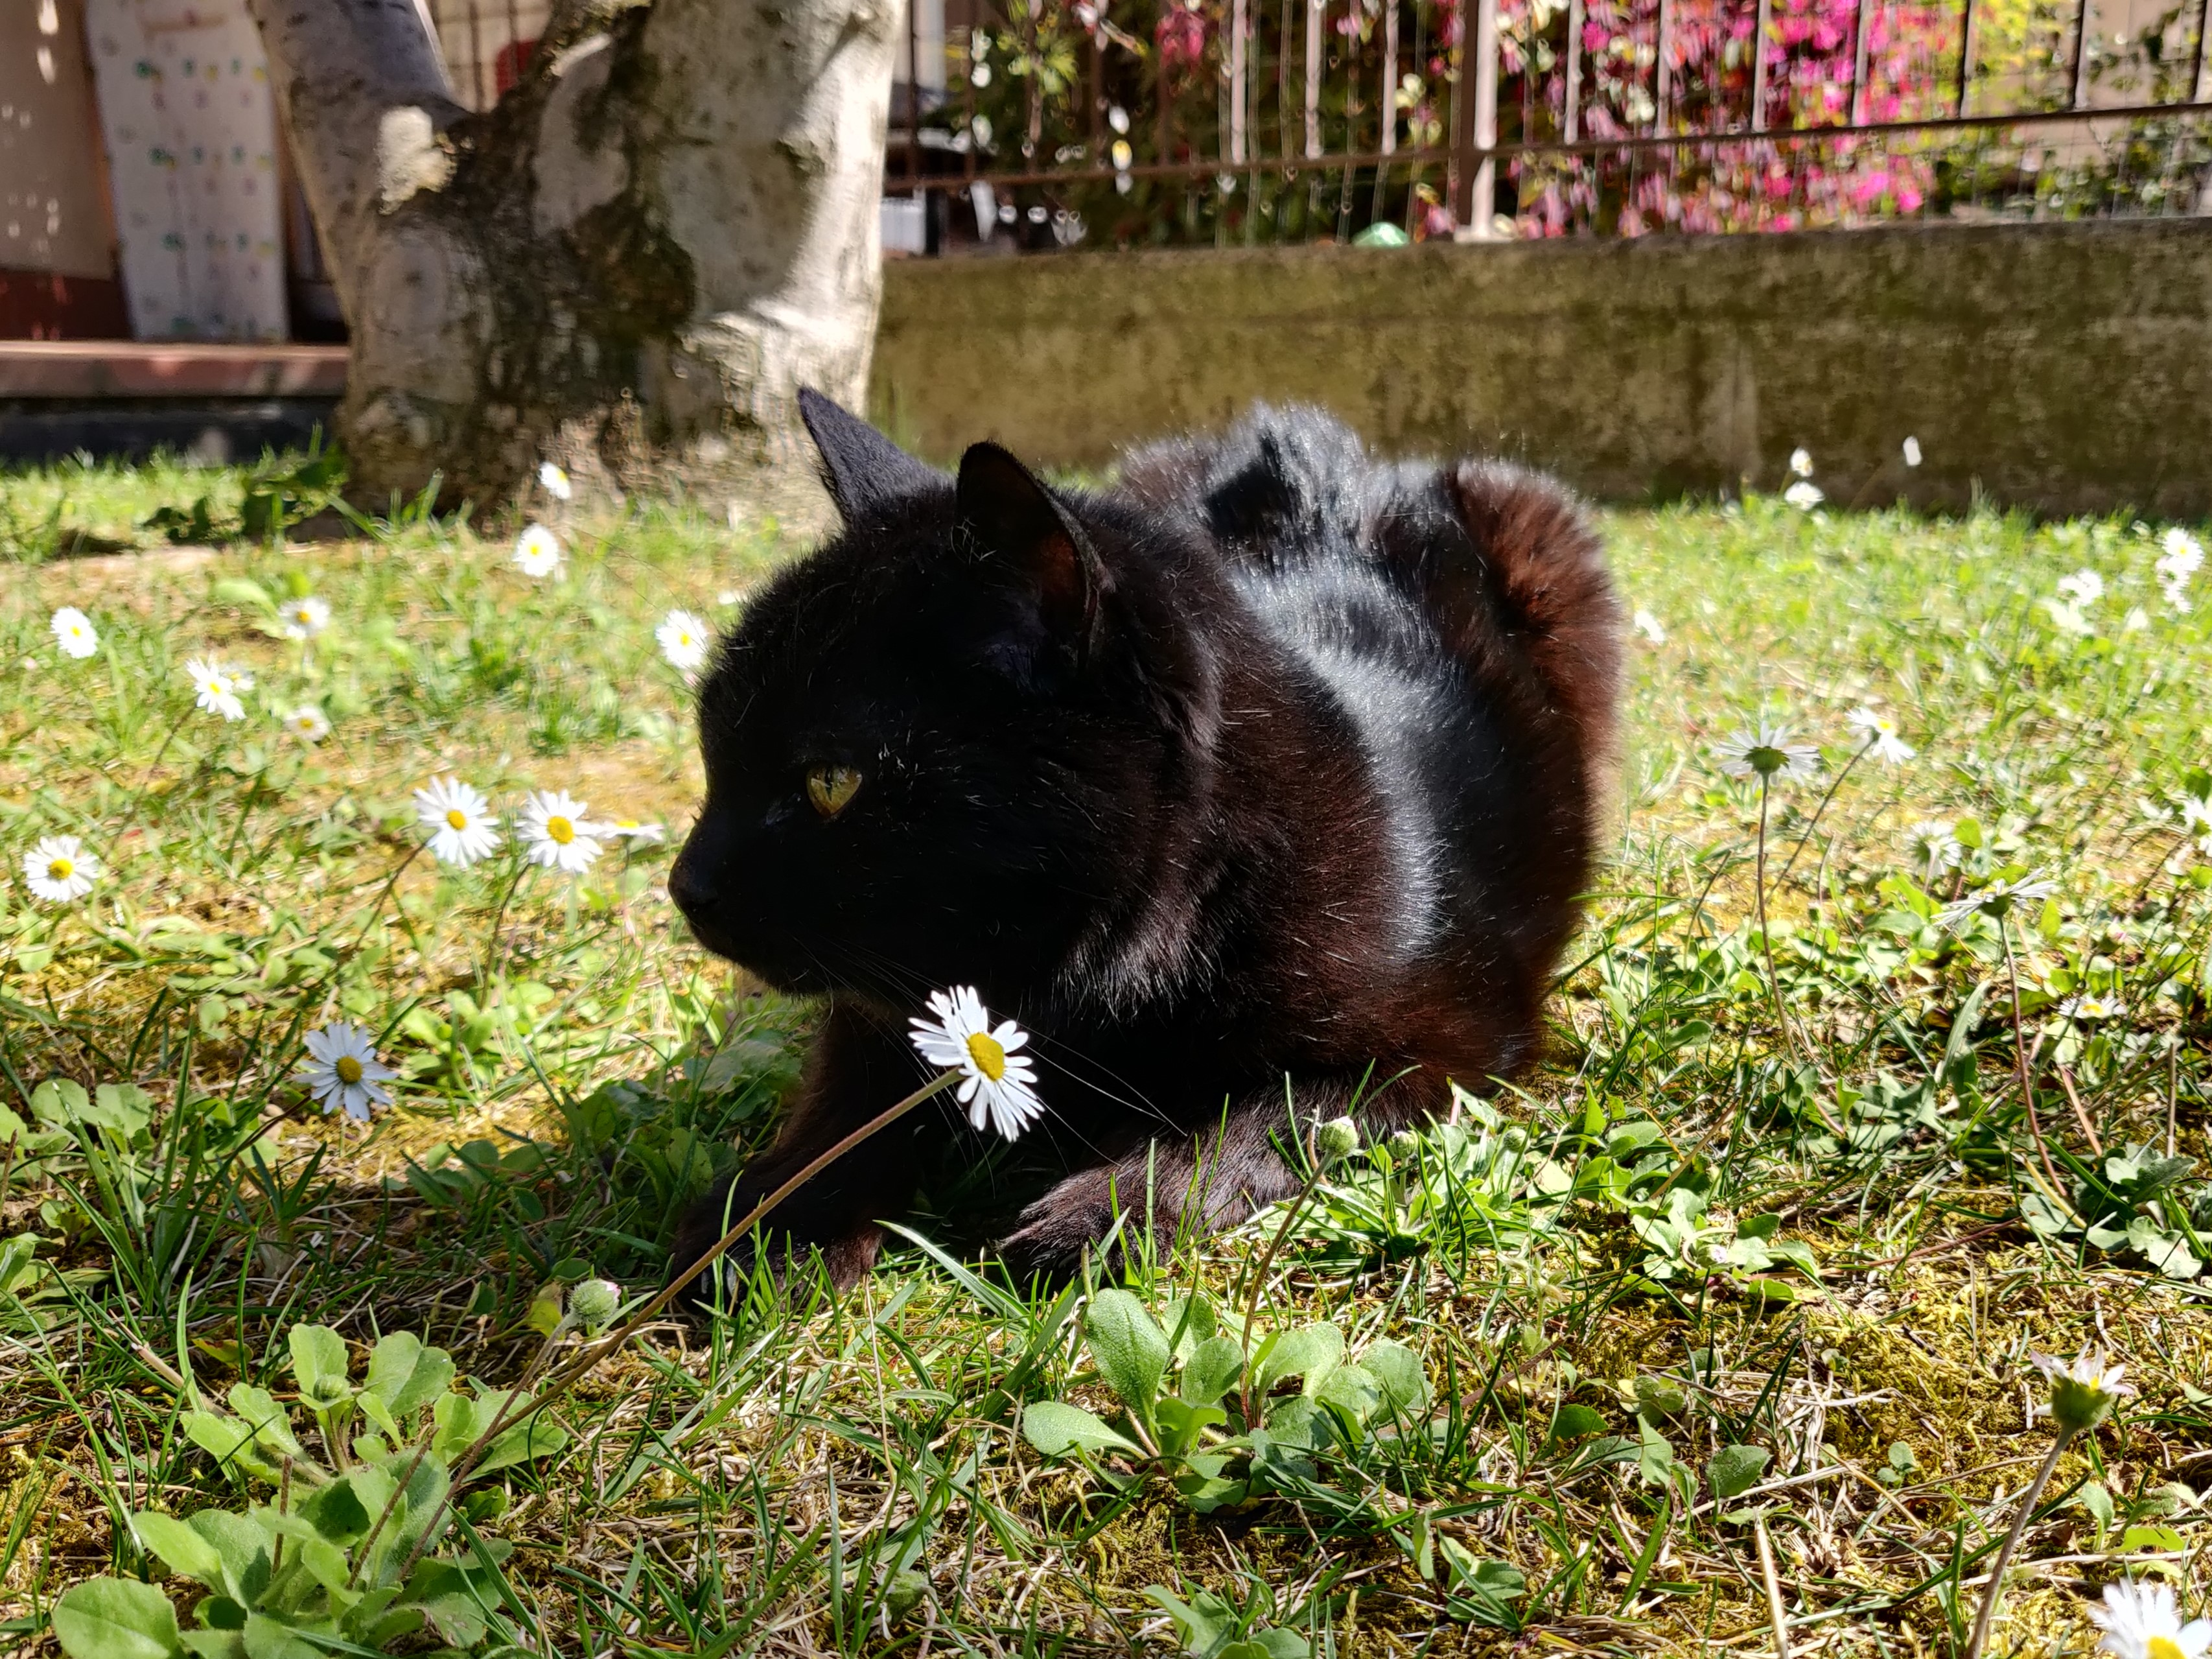
\includegraphics[width=0.7\linewidth]{Immagini/micia_cut.jpg}
% \end{figure}

% \begin{figure}[h]
% \hfill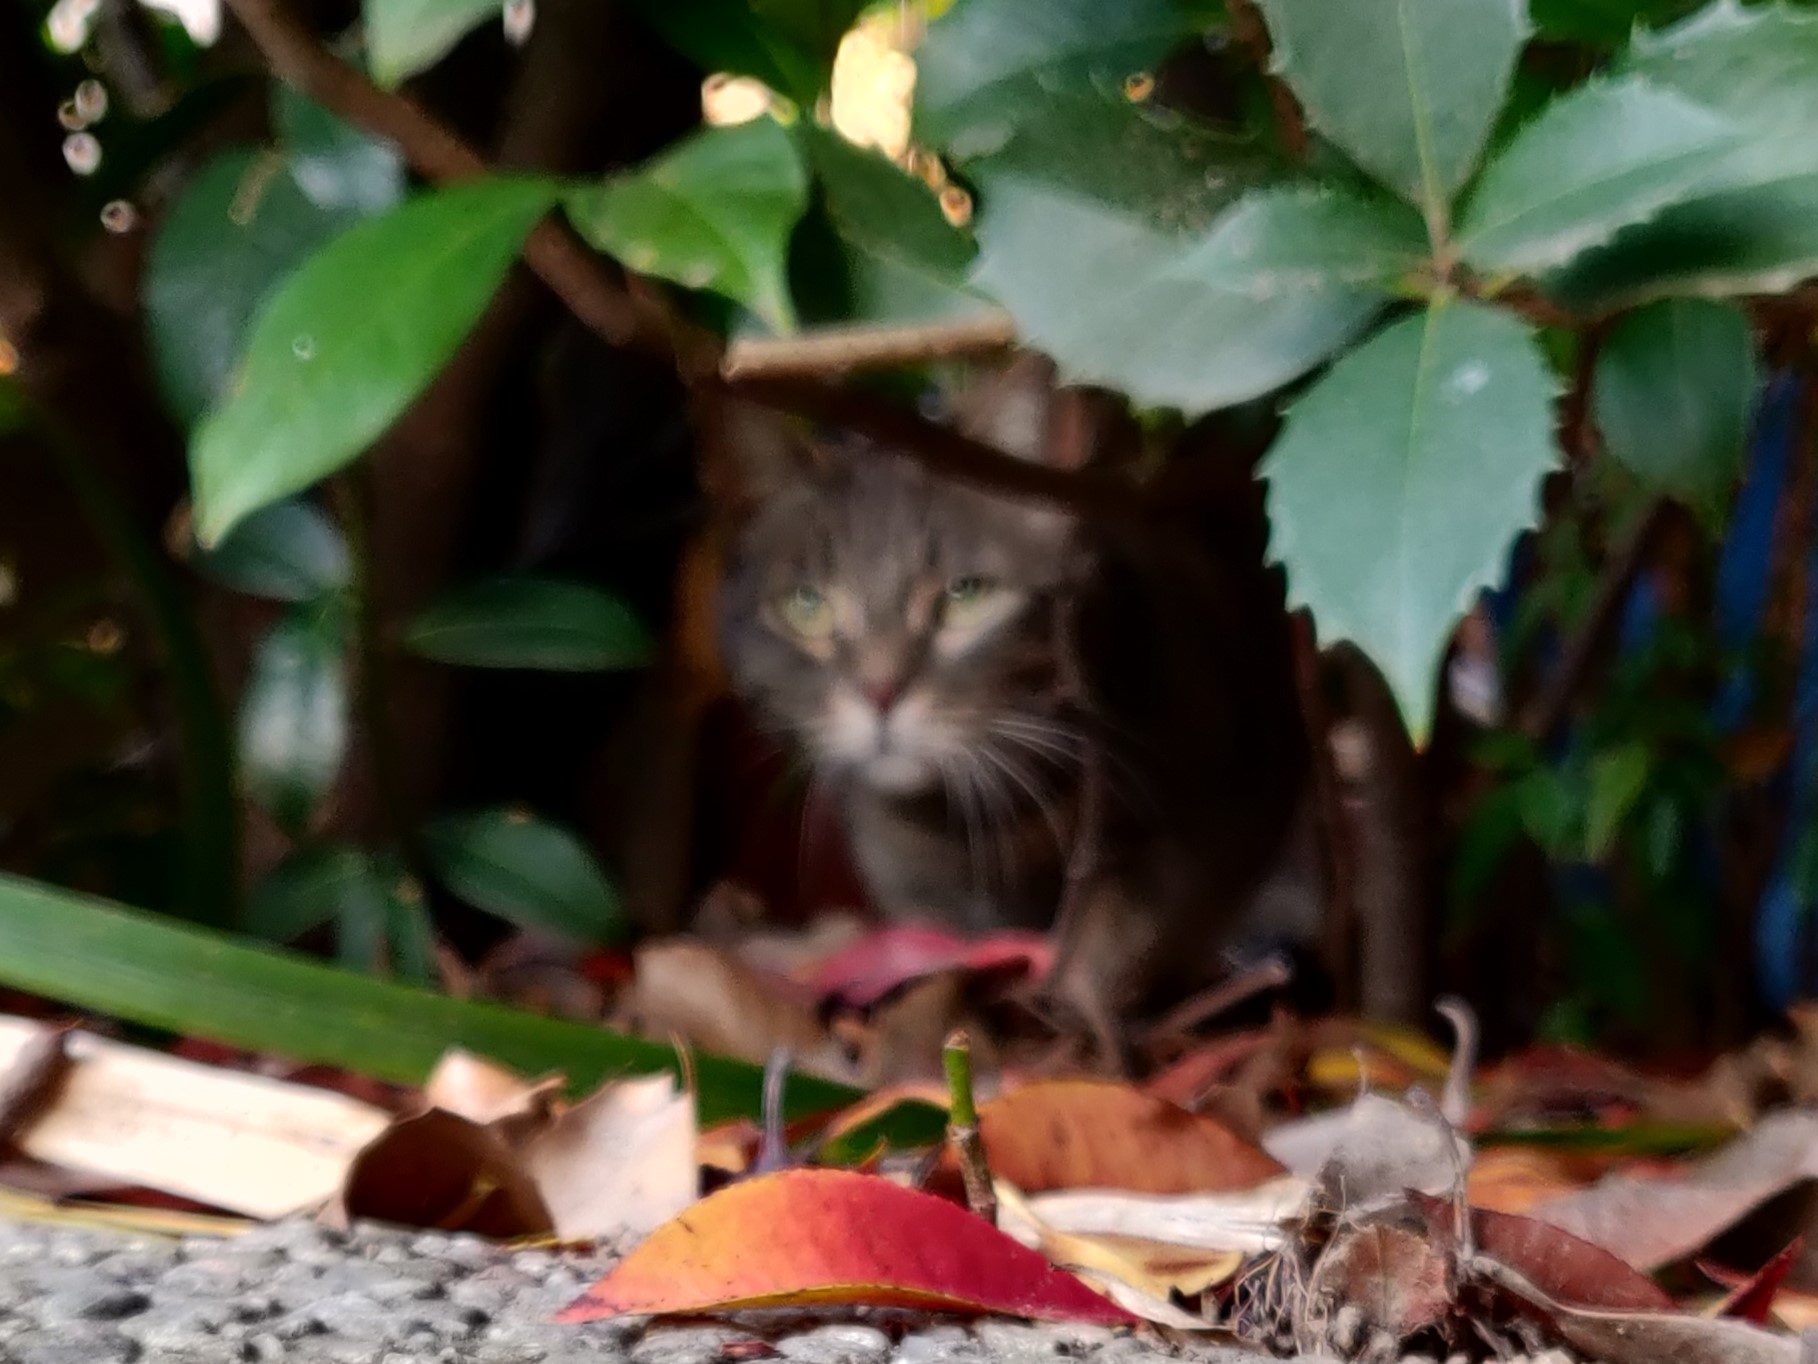
\includegraphics[width=0.7\linewidth]{Immagini/micio_1.jpg}
% \end{figure}

\end{flushright}
\vspace{\stretch{2.3}}

\cleardoublepage

\pdfbookmark[1]{Abstract}{Abstract}
\chapter*{Abstract}

Clustering is a key technique for identifying patterns and structures in complex datasets, whose relevance is intensified in spatio-temporal contexts where observations are simultaneously influenced by multiple factors such as space, time, and covariates. To this end, the Dependent Random Partition Model (DRPM) is one of the most relevant bayesian models due to its explicit consideration of temporal dependence in the partitions. However, the current implementation lacks of the inclusion of covariates, the handling of missing data, and the efficiency in execution times. Therefore, in this work we improve the original DRPM model by addressing those issues trough updates on the model formulation and a brand new implementation in Julia. These advancements are then tested on synthetic and real-world datasets, including air quality data from the AgrImOnIA project in Lombardy, Italy.

\textsc{Keywords:} bayesian modelling, clustering, spatio-temporal data, computational statistics


\cleardoublepage

\pdfbookmark[1]{Sommario}{Sommario}
\chapter*{Sommario}

\selectlanguage{italian}
Il clustering è una tecnica fondamentale per identificare strutture e pattern in dataset complessi, la cui importanza è intensificata nei contesti spazio-temporali in cui le osservazioni sono influenzate simultaneamente da molteplici fattori come spazio, tempo e covariate. In tal senso, il modello DRPM (Dependent Random Partition Model, modello per partizioni aleatorie dipendenti) è uno dei modelli bayesiani più rilevanti in quanto tiene conto in modo esplicito della dipendenza temporale delle partizioni. Tuttavia, l'attuale implementazione manca dell'inclusione di covariate, della gestione dei dati mancanti, e di efficienza nei tempi di esecuzione. In questo lavoro abbiamo quindi migliorato l'originale modello DRPM affrontando tali problemi tramite aggiornamenti sulla formulazione del modello e una fiammante implementazione in Julia. Questi sviluppi sono stati poi testati su dataset sintetici e reali, compresi i dati sulla qualità dell'aria in Lombardia del progetto AgrImOnIA.

\textsc{Parole chiave:} modello bayesiano, clustering, dati spazio-temporali, statistica computazionale

\selectlanguage{english}

\cleardoublepage

\pdfbookmark[1]{Contents}{Contents}
% \begin{spacing}{0.9}
    \tableofcontents
% \end{spacing}


\listoffigures
\listoftables
% \listofalgorithms
% \lstlistoflistings




% --------------------------------------- %
% 	MAINMATTER
% --------------------------------------- %
\cleardoublepage
\mainmatter
% \input{MainMatter/Introduzione}
% \input{MainMatter/StatoArte}
% \input{MainMatter/ProveSperimentali}
% \input{MainMatter/AnalisiNumeriche}
% \input{MainMatter/Conclusioni}

\chapter{Introduction}

Clustering has always been a powerful tool to identify structures and patterns in data especially in contexts where relationships between the observations are complex, e.g. when the target variable is affected by many factors simultaneously. For this reason, clustering techniques saw a continuos increase in popularity in a variety of scientific fields, including social sciences, climate and environmental analysis, economics, and healthcare. The importance of clustering becomes even more noticeable when working on spatio-temporal datasets, in which observations are collected over time and across different spatial locations, possibly concealing trends behind both information levels. This type of data, in fact, is inherently complex due to this dependence and interaction between spatial and temporal dimensions; a complexity that is further increased if covariates are also available. For that reason, an effective analysis of such data demands models that can account for this dependence while also providing efficient implementations to be possibly applied on large scale datasets, which are commonly accessible in this context.

Recently, the use of bayesian methods to perform clustering has gained some attention, particularly in this field of spatio-temporal datasets. Bayesian clustering, in fact, allows to incorporate prior information into the model enhancing the flexibility and interpretability of the results with respect, for example, to more traditional frequentist approaches. Throughout the years, several models have been developed, but one of the most relevant to this end is the Dependent Random Partition Model (DRPM), which stands out for being able to handle explicitly the temporal dependence of partitions into the model formulation, while also possibly accounting for the spatial information. However, the current DRPM implementation, written in C and available trough an R interface, lacks some relevant utilities such as the inclusion of covariates, which could further improve the generation and informativity of the clusters, the handling of missing data, and an efficient implementation, which would speed up the model fitting to e.g. run multiple chains in parallel of be more easily applied on large scale datasets.

In this work, we aim to address these three issues by enlarging the original model, that is, preserving the primary idea of the formulation but making it richer trough the insertion of new components. We will show how this updated model can perform better than the original one, under the same testing conditions, and can also improve the clustering accuracy and interpretation trough the inclusion of covariates. All this while also providing faster execution times. In fact, implementing the model using the Julia language, rather than C, we took advantage of its high-performance capabilities and well-equipped statistical ecosystem. Our comparison will focus on both synthetic datasets and real-world applications, with the latter involving air quality measurements from the AgrImOnIA dataset, a comprehensive record of air pollutant levels and other environmental variables measured across the Lombardy region of Italy.

Chapter \ref{cap: description of the model} will briefly review the literature about bayesian clustering models and then dive deeply into the analysis and description of DRPM, and of our updated version, about their core aspects of sampling algorithm, spatial cohesions, and covariates similarities.

Chapter \ref{Implementation and optimizations} will provide some insights about the computational aspects of the model implementation, motivating the choice of the Julia language and reporting the optimizations possibilities emerged when developing the algorithm.

Chapter \ref{chap: testing} will be devoted to test and compare the original DRPM formulation and implementation to our updated version. We will check if they perform similarly, at a common testing level, and assess the performances of our model when we employ the new updates, i.e. the handling of missing data and the insertion of covariates at clustering and likelihood levels. An analysis about expected execution  times with respect to the size of the dataset will also be provided.
 
Finally, in Chapter \ref{chap: conclusion}, we will briefly review the benefits and drawbacks that this work revealed and suggest possible further improvements or development paths.

% \setlength\epigraphwidth{0.7\textwidth}
% \epigraph{\itshape
% So this is all my introduction. I fully agree that it is quite unnecessary, but since it is already written, I shall let it stand. And now let’s get down to business.
% }{--- F\"{e}dor Dostoevskij, \textit{Brothers Karamazov}}
% % }{--- \textsc{F\"{e}dor Dostoevskij}, Notes from the Underground}
% \setlength\epigraphwidth{0.8\textwidth}



% \setlength\epigraphwidth{0.7\textwidth}
% \epigraph{\itshape
% So this is all my introduction. I fully agree that it is quite unnecessary, but since it is already written, I shall let it stand. And now let’s get down to business.
% }{--- F\"{e}dor Dostoevskij, \textit{Brothers Karamazov}}
% % }{--- \textsc{F\"{e}dor Dostoevskij}, Notes from the Underground}
% \setlength\epigraphwidth{0.8\textwidth}

% \setlength\epigraphwidth{.7\textwidth}
% \epigraph{\itshape
% So this is all my introduction. I fully agree that it is quite unnecessary, but since it is already written, I shall let it stand. And now let’s get down to business.
% }{--- F\"{e}dor Dostoevskij, \textit{Brothers Karamazov}}
% \setlength\epigraphwidth{.8\textwidth}



\chapter{Description of the model}
\label{cap: description of the model}

\epigraph{\itshape
% Well, gentlemen, why don't we reduce all this reasonableness to dust with one good kick, for the sole purpose of sending all these logarithms to the devil and living once more according to our own stupid
% will!” 
% "I say, gentleman, hadn't we better kick over the whole show and scatter rationalism to the winds, simply to send these logarithms to the devil, and to enable us to live once more at our own sweet foolish will!"
% "Come on, gentlemen, why shouldn't we get rid of all this calm reasonableness with one kick, just so as to send all these logarithms to the devil and be able to live our own lives at our own sweet will?"
"Come on, gentlemen, why shouldn't we get rid of all this calm reasonableness with one good kick, just so as to send all these logarithms to the devil and be able to live our own lives at our own sweet will?"
% ma non penso verrà approvata l'idea di inserirla
% mi piaceva solo perché mi piace dostoevskij e perché lì cita i logaritmi, che appaiono anche nell'algoritmo di campionamento quando si usa metropolis
}{--- F\"{e}dor Dostoevskij, \textit{Notes from the Underground}}
% }{--- \textsc{F\"{e}dor Dostoevskij}, Notes from the Underground}

In the bayesian framework, clustering is possible by employing a random probability measure of discrete type that induces a distribution over random partitions. This discreteness is obtained with the Dirichlet Process (DP), which several clustering models implement either trough the stick-breaking representation \cite{stick-br1} \cite{stick-br2} \cite{stick-br3} \cite{stick-br4} \cite{stick-br5} \cite{stick-br6} \cite{stick-br7} or trough the P\'{o}lya urn scheme \cite{polya-competitor}. However, these classical bayesian methods rely on modelling the dependence in the random partitions by modelling the dependence inside the random probability measures, i.e. on the parameters which underlie those DP representations rather than to the clusters themselves. This approach is therefore kind of a "step back" from the main object of interest, the clusters, which are then only \textit{induced} by the random partition model. As a consequence, there is no guarantee that the correlation that appears in the parameters would subsequently reflect into correlation among the partitions, often producing counterintuitive behaviours in the results. The Dependent Random Partition Model (DRPM) \cite{1-drpm}, on the other hand, models \textit{directly} the sequence of partitions, thus providing a more reasonable, accurate, and interpretable temporal evolution of the clusters.

Before diving into the model description, we define some notation conventions. We setup in a spatio-temporal context with $i=1,\ldots,n$ and $t=1,\ldots,T$ being the indexes for units and time instants. We will denote with $\rho_t=\{S_{1t}, \ldots, S_{k_tt}\}$ the partition at time $t$, of the $n$ experimental units, composed by $k_t$ cluster. Another possible representation of the partition is trough cluster membership labels $\vec{c}_t = \{ c_{1t}, \ldots, c_{nt}\}$, where $c_{it}=j$ if unit $i$ belongs to cluster $S_{jt}$. Finally, we will denote with a $\star$ superscript all the variables or quantities which are cluster-specific.

To implement dependence in the partitions one could simply propose a joint probability model for $(\rho_1, \ldots, \rho_T)$, denoted as $P(\rho_1, \ldots, \rho_T)$, where each $\rho_t$ is set to be possibly affected by all the other partitions. This principle, however, it's far too complex and general to be modelled efficiently; therefore the DRPM authors limited this temporal connection to a first-order Markov-chain structure, where the conditional distribution of $\rho_t$ given all the predecessors $\rho_{t-1}, \rho_{t-2}, \ldots, \rho_1$ actually depends only on $\rho_{t-1}$. This brings the random partition model to the form
\begin{equation}
P(\rho_1, \ldots, \rho_T) = P(\rho_T|\rho_{T-1}) \cdots P(\rho_2|\rho_1) P(\rho_1)
\end{equation}
To explicitly manage the relation between $\rho_t$ and $\rho_{t-1}$ some auxiliary variables are introduced. The idea is that if two partitions are highly time-dependent, few changes will occur between them. In turn, partitions which are quite independent will possibly exhibit very different configurations. To express this fixity or flexibility concept, for each unit $i=1,\ldots,n$ the following variable is introduced\footnote{a quick way to remind this convention is thinking that $\gamma_{it}$ answers to the question "do I stay fixed?" asked from unit $i$ perspective.}
\begin{equation}
\gamma_{it} = \begin{cases}
    1 & \text{if unit $i$ is \emph{not} reallocated when moving from time $t-1$ to $t$} \\
    0 & \text{otherwise (i.e. unit \emph{is} reallocated)}
\end{cases}
\end{equation}
By construction, we set $\gamma_{i1}=0$ for all $i$, meaning that at the first time instant all units will get reallocated since they have no partition to which they could be possibly fixed at. Regarding their modelling, the authors proposed $\gamma_{it} \simind \Ber(\alpha_t)$ with $\alpha_t \in [0,1]$ behaving as a temporal dependence parameter. At the two extremes, $\alpha_t=1$ will denote perfect temporal dependence, with $\rho_t = \rho_{t-1}$, while $\alpha_t=0$ will imply full independence of $\rho_t$ from $\rho_{t-1}$. The parameter $\alpha_t$ can actually be global, and we will write simply $\alpha$ without any subscripts, or instead time and/or unit specific, offering the cases of $\alpha_t$, $\alpha_i$, or $\alpha_{it}$. For the sake of clarity, the vector $\vec{\gamma}_t = (\gamma_{1t},\ldots,\gamma_{nt})$ is created, and the augmented joint model becomes in the form
\begin{equation}
P(\vec{\gamma}_1,\rho_1, \ldots, \vec{\gamma}_T,\rho_T) = P(\rho_T|\vec{\gamma}_T,\rho_{T-1})P(\vec{\gamma}_T) \cdots P(\rho_2|\vec{\gamma}_2,\rho_1)P(\vec{\gamma}_2) P(\rho_1) \label{trpm}
\end{equation}


The insertion of these additional variables makes the model very powerful in describing the temporal dependence of the partitions but slightly hinders the design of the sampling algorithm. To outline it, we firstly need a 
\begin{definition}[compatibility]
Two partitions $\rho_t$ and $\rho_{t-1}$ are \textit{compatible} with respect to $\vec{\gamma}_t$ if $\rho_t$ can be obtained from $\rho_{t-1}$ by reallocating items as indicated by $\gamma_t$; i.e. only moving the units $i$ with $\gamma_{it}=0$. 
\end{definition}
To perform this compatibility check, it is enough to ensure that the reduced partitions from $\rho_t$ and $\rho_{t-1}$ are the same, with reduced meaning their restriction to the units which cannot move. Indeed, if those fixed units are clustered in the same ways, then surely the free-movers from $\rho_{t}$ can be set to match the labels assigned by partition $\rho_{t-1}$. Denoting as $\mathfrak{R}_t= \{ i : \gamma_{it}=1\}$ the set of fixed units at time $t$, this check translates into asking that $\rho_t^{\mathfrak{R}_t} = \rho_{t-1}^{\mathfrak{R}_t}$.

The sampling algorithm requires that when we are drawing the new samples for the $\gamma_{it}$a, or also for the cluster labels $c_{it}$, we firstly need to check if those draws can actually be valid, i.e. if they would keep compatible and coherent all the partitions and parameters involved. For example, when updating $\gamma_{it}$ during each iteration $d$ of the algorithm, the only case which can raise problems is when we pass from $\gamma_{it}^{(d-1)}=0$ to $\gamma_{it}^{(d)}=1$. This step corresponds to the case in which a unit $i$ that was initially (i.e. according to the previous iteration parameters) free to be reassigned is now instead deemed to stay fixed in her cluster. However, this change may not align to the current sampled values of the partitions $\rho_{t-1}^{(d)}$ and $\rho_t^{(d-1)}$. Therefore, compatibility between their reductions to the units in the set $\mathfrak{R}_t \cup \{i\}$ needs to be checked and, if this check fails, the tentative update $\gamma_{it}^{(d-1)}=0 \to \gamma_{it}^{(d)}=1$ is not allowed to be performed and we force $\gamma_{it}^{(d)}=0$ in the sampling algorithm. Similar checks are conducted when $\rho_t$ is updated. In this step, only the units that can actually move, i.e. that have $\gamma_{it}=0$, are updated, and therefore there are no compatibility problems between $\rho_{t-1}$ and $\rho_t$. However, since the update of $\gamma_{it}$ occurs before the one of the partition, compatibility needs to be checked between $\rho_{t}$ and $\rho_{t+1}$. 
% The compatibility check and the relabeling process of the clusters, needed to control the label-switching problem of bayesian clustering models, are also the main reason of the ... slowness of the code vabe non importa dirlo ora

In any case, once the partition model is specified, there is great flexibility in how to setup the rest of the hierarchical model. To allow temporal dependence to propagate trough the model, an autoregressive $\text{AR}(1)$ component is also added to the formulation of the model (but only optionally in the implementation), both at the data and cluster-specific parameters level. All this led the authors to the following complete model
\begin{align*}
% \begin{split}
Y_{it}|Y_{it-1},\vec{\mu}^{\star}_t,\vec{\sigma}^{2\star}_t, \vec{\eta},\vec{c}_t &\simind \mathcal{N}(\mu_{c_{it}t}^\star+\eta_{1i}Y_{it-1},\sigma^{2\star}_{c_{it}t}(1-\eta_{1i}^2)) \\
Y_{i1} &\simind \mathcal{N}(\mu^\star_{c_{i1}1},\sigma^{2\star}_{c_{i1}1})\\
% &\text{for } i=1,\ldots,n\text{ and } t=2,\ldots,T\\
%
\xi_i = \text{Logit$(\tfrac{1}{2}(\eta_{1i}+1)$}) &\simind \text{Laplace$(a,b)$}\\
%
( \mu_{jt}^\star, \sigma_{jt}^\star) &\simind \N(\theta_t,\tau_t^2) \times \U(0,A_\sigma)\\
%
\theta_t | \theta_{t-1} &\simind \N((1-\phi_1)\phi_0 + \phi_1\theta_{t-1},\lambda^2(1-\phi_1^2))\\
%
(\theta_1,\tau_t) &\simiid \N(\phi_0,\lambda^2) \times \U(0,A_\tau)\\
%
(\phi_0,\phi_1,\lambda) &\sim \N(m_0,s_0^2) \times \U(-1,1) \times \U(0,A_\lambda)\\
%
\{\vec{c}_t, \ldots, \vec{c}_T\} &\sim \text{tRPM}(\vec{\alpha}, M) \text{ with } \alpha_t \simiid \text{Beta}(a_\alpha, b_\alpha)
\tag{\stepcounter{equation}\theequation}
% \end{split}
\end{align*}
where $\text{tRPM}$ represents the temporal random partition model \eqref{trpm}.

Moving towards our update, we decided to refine some parts of that formulation. Regarding the variances $\sigma^{2\star}_{jt}$, $\tau^2_t$, and $\lambda^2$, we chose to model them trough an inverse gamma distribution rather than the uniform employed originally. This is indeed a more sophisticate choice, since the tuning of the parameters of an $\invgamma(a,b)$ is a bit more difficult than simply setting the bounds of a $\U(l,u)$, but should guarantee a better mixing in the chain. In fact, the $\invgamma$ distributions recovers conjugacy in the model, thanks to the normal law assigned to the other parameters, allowing the update step of the variances to be performed trough the analytically exact Gibbs sampler rather than the acceptance-rejection method of Metropolis algorithm. Finally, to improve the accuracy in fitting the target values, we added a regression parameter $\vec{\beta}_t$ in the likelihood. We decided to make it only time-dependent, and not also unit-dependent, to lighten the already quite-heavy formulation.

The final updated model is now proposed, with highlighted in dark red the changes and insertions that we made.
\begin{align*}
% \begin{split}
Y_{it}|Y_{it-1},\vec{\mu}^{\star}_t,\vec{\sigma}^{2\star}_t, \vec{\eta},\vec{c}_t &\simind \mathcal{N}(\mu_{c_{it}t}^\star+\eta_{1i}Y_{it-1} + \alert{\vec{x}_{it}^T\vec{\beta}_t},\sigma^{2\star}_{c_{it}t}(1-\eta_{1i}^2)) \\
Y_{i1} &\simind \mathcal{N}(\mu^\star_{c_{i1}1}+ \alert{\vec{x}_{i1}^T\vec{\beta}_1},\sigma^{2\star}_{c_{i1}1})\\
% &\text{for } i=1,\ldots,n\text{ and } t=2,\ldots,T\\
%
\alert{\vec{\beta}_t} &\; \alert{\simind} \; \alert{\N_p(\vec{b},s^2 I)}\\
\xi_i = \text{Logit$(\tfrac{1}{2}(\eta_{1i}+1)$}) &\simind \text{Laplace$(a,b)$}\\
%
( \mu_{jt}^\star, \alert{\sigma_{jt}^{2\star}}) &\simind \N(\theta_t,\tau_t^2) \times \alert{\invgamma(a_\sigma,b_\sigma)}\\
%
\theta_t | \theta_{t-1} &\simind \N((1-\phi_1)\phi_0 + \phi_1\theta_{t-1},\lambda^2(1-\phi_1^2))\\
%
(\theta_1,\alert{\tau_t^2}) &\simiid \N(\phi_0,\lambda^2) \times  \alert{\invgamma (a_\tau,b_\tau)}\\
%
(\phi_0,\phi_1,\alert{\lambda^2}) &\sim \N(m_0,s_0^2) \times \U(-1,1) \times \alert{\invgamma (a_\lambda,b_\lambda)}\\
%
\{\vec{c}_t, \ldots, \vec{c}_T\} &\sim \text{tRPM}(\vec{\alpha}, M) \text{ with } \alpha_t \simiid \text{Beta}(a_\alpha, b_\alpha)
 \numberthis \label{jdrpm model}
% \end{split}
\end{align*}

A visual representation of this new version of the DRPM model is also present in Figure \ref{fig: model graph}, to more clearly appreciate the hierarchical structure and the relations among the parameters.

% \begin{center}
\begin{figure}[!ht]
    % \hspace{-36pt} 
    \centering
     \hspace*{-0.04\linewidth}
\begin{tikzpicture}
\begin{scope}[every node/.style={align=center}]
% \begin{scope}[every node/.style={draw,align=center}]
    \node (Y) at (0,10.5) {
    $Y_{it}\sim \mathcal{N}(\mu_{c_{it}t}^\star+\eta_{1i}Y_{it-1} + \alert{\vec{x}_{it}^T\vec{\beta}_t},\sigma^{2\star}_{c_{it}t}(1-\eta_{1i}^2))$ 
    \\ 
    $Y_{i1} \sim \mathcal{N}(\mu^\star_{c_{i1}1} + \alert{\vec{x}_{i1}^T\vec{\beta}_1},\sigma^{2\star}_{c_{i1}1})$
    };
    \node (eta1) at (3,7) {$\xi_i = \text{Logit$(\tfrac{1}{2}(\eta_{1i}+1)$}) \sim \text{Laplace$(a,b)$}$};
    \node (sigma) at (-6,8) {$\sigma_{jt}^{2\star} \sim \alert{\invgamma(a_\sigma, b_\sigma)}$};
    \node (beta) at (6,8) {\alert{$\vec{\beta}_t \sim \N_p(\vec{b},s^2 I)$}};
    \node (mu) at (-3,7) {$\mu_{jt}^\star \sim \N(\theta_t,\tau_t^2)$};

    \node (tau) at (-4,4) {$\tau^2_t \sim \alert{\invgamma(a_\tau,b_\tau)}$};
    \node (theta) at (3,4) {$\theta_t \sim \N((1-\phi_1)\phi_0 + \phi_1\theta_{t-1},\lambda^2(1-\phi_1^2))$\\$\theta_1 \sim \N(\phi_0,\lambda^2)$};

   \node (internals) at (-6.5,2.3){\color{Gray}$\alpha_{(it)} \sim \text{Beta}(a_{\alpha(i)}, b_{\alpha(i)})$\\\color{Gray}$ \gamma_{it}\simind \text{Ber}(\alpha_{(it)})$};

    \node (phi0) at (-3,1){$\phi_0\sim \N(m_0,s_0^2)$};
    \node (phi1) at (1,1) {$\phi_1\sim \U(-1,1)$};
    \node (lam2) at (5,1) {$\lambda^2 \sim \alert{\invgamma (a_\lambda,b_\lambda)}$};

    
\end{scope}
% \begin{scope}[>={Stealth[black]},
\begin{scope}[>={latex[black]},
              % every node/.style={fill=white,circle},
              every edge/.style={draw=black,thick}]
    \path [->] (Y) edge (eta1);
    \path [->] (Y) edge (mu);
    \path [->] (Y) edge (sigma);
    \path [->] (Y) edge (beta);
    
    \path [->] (mu) edge (tau);
    \path [->] (mu) edge (theta);
    
    \path [->] (theta) edge (phi0);
    \path [->] (theta) edge (phi1);
    \path [->] (theta) edge (lam2);
    
    % \path [->] (eta1) edge[bend right=60] node {$1$} (E); 
\end{scope}
\end{tikzpicture}
% \vspace{2pt}
    \caption[Updated DRPM model graph]{Graph visualization of the DRPM model, with highlighted in dark red the changes that we made to the original formulation and in gray the internal variables of the model.}
    \label{fig: model graph}
\end{figure}
% \end{center}

In the course of this work, for the sake of clarity, we will refer to CDRPM for the original model formulation of \cite{1-drpm} and to JDRPM for our updated version. 

We will now dive more deeply into the characteristics of the models by deriving the update rules for the parameters which will be used to implement the MCMC fitting algorithm and, subsequently, inspecting the behaviours of the spatial cohesions and covariates similarities.

\section{Update rules derivation}
We briefly report the full conditionals derivation for the parameters which had a conjugacy in the model (for the full computations see Appendix \ref{app: theoretical details}). The other variables not included here, namely $\eta_{1i}$ and $\phi_1$, involved instead the classical Metropolis update.

\begin{itemize}

\item update $\sigma^{2\star}_{jt}$
\begin{align*}
% \begin{split}
&\text{for $t=1$} \text{: }
  f(\sigma^{2\star}_{jt}|-)\propto \text{kernel of a $\invgamma(a_{\postp{\sigma}}, b_{\postp{\sigma}})$ with}\\
&a_{\postp{\tau}}= a_\sigma + \frac{|S_{jt}|}{2} \quad
%
b_{\postp{\tau}}=b_\sigma + \frac{1}{2}\sum_{i \in S_{jt}}(Y_{it}-\mu^\star_{jt}-\vec{x}_{it}^T\vec{\beta}_t)^2 \\
% \end{split}
% \begin{split}
&\text{for $t>1$}\text{: }
  f(\sigma^{2\star}_{jt}|-) \propto \text{kernel of a $\invgamma(a_{\postp{\sigma}}, b_{\postp{\sigma}})$ with}\\
&a_{\postp{\tau}}= a_\sigma + \frac{|S_{jt}|}{2} \quad
%
b_{\postp{\tau}}=b_\sigma + \frac{1}{2}\sum_{i \in S_{jt}}(Y_{it}-\mu^\star_{jt}-\eta_{1i}Y_{it-1}-\vec{x}_{it}^T\vec{\beta}_t)^2 
% \tag{\stepcounter{equation}\theequation}
 \numberthis \label{update sigma2h}
% \end{split}
\end{align*}


\item update $\mu^\star_{jt}$
\begin{align*}
% \begin{split}
&\text{for $t=1$} \text{: }
 f(\mu^\star_{jt}|-) \propto \text{kernel of a $\N(\mu_{\postp{\mu^\star_{jt}}},\sigma^2_{\postp{\mu^\star_{jt}}})$ with}\\
&\sigma^2_{\postp{\mu^\star_{jt}}}=\frac{1}{\frac{1}{\tau^2_t}+\frac{|S_{jt}|}{\sigma^{2\star}_{jt}}}\quad
% \sigma^2_{\postp{\mu^\star_{jt}}}&=1 \bigg/ \left[ \tau^2_t+\frac{|S_{jt}|}{\sigma^{2\star}_{jt}}\right]\\
%
\mu_{\postp{\mu^\star_{jt}}}=\sigma^2_{\postp{\mu^\star_{jt}}}\left( \frac{\theta_t}{\tau_t^2} + \frac{\sum_{i \in S_{jt}} (Y_{i1}-\vec{x}_{it}^T\vec{\beta}_t)}{\sigma^{2\star}_{jt}} \right)\\
% \begin{split}
&\text{for $t>1$} \text{: }
 f(\mu^\star_{jt}|-) \propto \text{kernel of a $\N(\mu_{\postp{\mu^\star_{jt}}},\sigma^2_{\postp{\mu^\star_{jt}}})$ with}\\
&\sigma^2_{\postp{\mu^\star_{jt}}}=\frac{1}{\frac{1}{\tau_t^2}+\frac{\sum_{i \in S_{jt}} \frac{1}{1-\eta_{1i}^2}}{\sigma^{2\star}_{jt}}}\quad
%
\mu_{\postp{\mu^\star_{jt}}}=\sigma^2_{\postp{\mu^\star_{jt}}}\left( \frac{\theta_t}{\tau_t^2} + \frac{\sum_{i \in S_{jt}} \frac{Y_{it}-\eta_{1i}Y_{i,t-1}-\vec{x}_{it}^T\vec{\beta}_t}{1-\eta_{1i}^2}}{\sigma_{jt}^{2\star}} \right)
 \numberthis \label{update muh}
% \tag{\stepcounter{equation}\theequation}
% \end{split}
\end{align*}


\item update $\vec{\beta}_t$
\begin{align*}
% \begin{split}
&  \text{for $t=1$} \text{: }
  f(\vec{\beta}_t|-) \propto \text{kernel of a $\N(\vec{b}_\post, A_\post)$ with}\\
 &A_\post = \left( \frac{1}{s^2}I + \sum_{i=1}^n \frac{\vec{x}_{it}\vec{x}_{it}^T}{\sigma^{2\star}_{c_{it}t}}\right)^{-1} \quad
\vec{b}_\post = A_\post \left( \frac{\vec{b}}{s^2} +\sum_{i=1}^n \frac{(Y_{it}-\mu^\star_{c_{it}t})\vec{x}_{it}}{\sigma^{2\star}_{c_{it}t}} \right) \\
&\text{i.e. } f(\vec{\beta}_t|-) \propto \text{kernel of a $\Ncan(\vec{h}_\post, J_\post)$ with}\\
&\vec{h}_\post = \left( \frac{\vec{b}}{s^2} +\sum_{i=1}^n \frac{(Y_{it}-\mu^\star_{c_{it}t})\vec{x}_{it}}{\sigma^{2\star}_{c_{it}t}} \right) \quad
J_\post = \left( \frac{1}{s^2}I + \sum_{i=1}^n \frac{\vec{x}_{it}\vec{x}_{it}^T}{\sigma^{2\star}_{c_{it}t}}\right)\\
% \begin{split}
& \text{for $t>1$} \text{: }
 f(\vec{\beta}_t|-) \propto \text{kernel of a $\N(\vec{b}_\post, A_\post)$ with}\\
 &A_\post = \left( \frac{1}{s^2}I + \sum_{i=1}^n \frac{\vec{x}_{it}\vec{x}_{it}^T}{\sigma^{2\star}_{c_{it}t}}\right)^{-1} \quad
\vec{b}_\post = A_\post \left( \frac{\vec{b}}{s^2} +\sum_{i=1}^n \frac{(Y_{it}-\mu^\star_{c_{it}t}- \eta_{1i}Y_{it-1})\vec{x}_{it}}{\sigma^{2\star}_{c_{it}t}} \right) \\
 &\text{i.e. } f(\vec{\beta}_t|-) \propto \text{kernel of a $\Ncan(\vec{h}_\post, J_\post)$ with}\\
&\vec{h}_\post = \left( \frac{\vec{b}}{s^2} +\sum_{i=1}^n \frac{(Y_{it}-\mu^\star_{c_{it}t}- \eta_{1i}Y_{it-1})\vec{x}_{it}}{\sigma^{2\star}_{c_{it}t}} \right) \quad
J_\post  = \left( \frac{1}{s^2}I + \sum_{i=1}^n \frac{\vec{x}_{it}\vec{x}_{it}^T}{\sigma^{2\star}_{c_{it}t}}\right)
 \numberthis \label{update betat}
% \tag{\stepcounter{equation}\theequation}
% \end{split}
\end{align*}
Here $\Ncan(\vec{h},J)$ is the canonical formulation of the $\N(\vec{\mu},\Sigma)$, with $\vec{h} = \Sigma^{-1}\vec{\mu}$ and $J = \Sigma^{-1}$. This other distribution facilitates the sampling, since these full conditional computations allow to derive directly the parameters of the canonical one, e.g. the inverse of the variance matrix rather than the variance matrix itself; and therefore sampling trough it does not require any inversion of matrices which would produce more computational load, numerical instabilities, and loss of accuracy. As a consequence, in Julia we can write
\mjline{rand(MvNormalCanon(h_star, J_star))}
rather than the riskier one
\mjline{rand(MvNormal(inv(J_star)*h_star, inv(J_star)))}; which apart from the previously mentioned disadvantages would be a statistically equivalent form.


\item update $\tau^2_t$
\begin{align*}
% \begin{split}
&f(\tau^2_t|-)\propto \text{kernel of a $\invgamma(a_{\postp{\tau}}, b_{\postp{\tau}})$ with}\\
&a_{\postp{\tau}}=\frac{k_t}{2}+a_\tau \quad
%
b_{\postp{\tau}}= \frac{\sum_{j=1}^{k_t}(\mu_{jt}^\star-\theta_t)^2}{2}+b_\tau
% \tag{\stepcounter{equation}\theequation}
 \numberthis \label{update tau2t}
% \end{split}
\end{align*}
    

\item update $\theta_t$
\begin{align*}
% \begin{split}
    \text{for }t=T &\text{: }
     f(\theta_t|-)\propto \text{kernel of a $\N(\mu_{\postp{\theta_t}},\sigma^2_{\postp{\theta_t}})$ with}\\
    \sigma^2_{\postp{\theta_t}}&=\dfrac{1}{\frac{1}{\lambda^2(1-\phi_1^2)}+\frac{k_t}{\tau_t^2}}\\
    \mu_{\postp{\theta_t}}&=\sigma^2_{\postp{\theta_t}}\left(\frac{\sum_{j=1}^{k_t}\mu^\star_{jt}}{\tau^2_t} + \frac{(1-\phi_1)\phi_0+\phi_1\theta_{t-1}}{\lambda^2(1-\phi_1^2)} \right)\\
% \begin{split}
    % \text{for $1<t<T$: }
\text{for } 1<t&<T \text{: }
     f(\theta_t|-)\propto \text{kernel of a $\N(\mu_{\postp{\theta_t}},\sigma^2_{\postp{\theta_t}})$ with}\\
    \sigma^2_{\postp{\theta_t}}&=\dfrac{1}{\frac{1+\phi_1^2}{\lambda^2(1-\phi_1^2)}+\frac{k_t}{\tau^2_t}}\\
    \mu_{\postp{\theta_t}}&=\sigma^2_{\postp{\theta_t}}\left(\frac{\sum_{j=1}^{k_t}\mu^\star_{jt}}{\tau^2_t} + \frac{\phi_1(\theta_{t-1}+\theta_{t+1}) + \phi_0(1-\phi_1)^2}{\lambda^2(1-\phi_1^2)} \right)\\
% \begin{split}
    \text{for }t=1 &\text{: }
     f(\theta_t|-)\propto \text{kernel of a $\N(\mu_{\postp{\theta_t}},\sigma^2_{\postp{\theta_t}})$ with}\\
    \sigma^2_{\postp{\theta_t}}&=\dfrac{1}{\frac{1}{\lambda^2}+\frac{\phi_1^2}{\lambda^2(1-\phi_1^2)}+\frac{k_t}{\tau^2_t}}\\
\mu_{\postp{\theta_t}}&=\sigma^2_{\postp{\theta_t}}\left(\frac{\phi_0}{\lambda^2}+\frac{\phi_1(\theta_{t+1}-(1-\phi_1)\phi_0)}{\lambda^2(1-\phi_1^2)}+\frac{\sum_{j=1}^{k_t}\mu^\star_{jt}}{\tau^2_t} \right)
% \tag{\stepcounter{equation}\theequation}
 \numberthis \label{update thetat}
% \end{split}
\end{align*}


\item update $\phi_0$
\begin{align*}
% \begin{split}
     f(\phi_0|-) &\propto \text{kernel of a $\N(\mu_{\phi_0\post},\sigma^{2}_{\phi_0\post})$ with}\\
    \sigma^{2}_{\postp{\phi_0}} &= \dfrac{1}{\frac{1}{s_0^2}+\frac{1}{\lambda^2}+\frac{(T-1)(1-\phi_1)^2}{\lambda^2(1-\phi_1^2)}}\\
    % \mu_{\phi_0\post} &= \sigma^{2}_{\phi_0\post} \left[\dfrac{m_0}{s_0^2}+\dfrac{\theta_1}{\lambda^2}+\dfrac{1-\phi_1}{\lambda^2(1-\phi_1^2)}\left( \sum_{t=2}^T \theta_t-\phi_1\theta_{t-1}\right)\right]
    \mu_{\phi_0\post} &= \sigma^{2}_{\phi_0\post} \left(\dfrac{m_0}{s_0^2}+\dfrac{\theta_1}{\lambda^2}+\dfrac{1-\phi_1}{\lambda^2(1-\phi_1^2)}\sum_{t=2}^T(\theta_t-\phi_1\theta_{t-1})\right)
% \tag{\stepcounter{equation}\theequation}
 \numberthis \label{update phi0}
% \end{split}
\end{align*}

\item update $\lambda^2$
% \begin{equation} \label{eq1}
\begin{align*}
% \begin{split}
     f(\lambda^2|-)&\propto \text{kernel of a $\invgamma(a_{\postp{\lambda}}, b_{\postp{\lambda}})$ with}\\
a_{\postp{\lambda}}&=\frac{T}{2}+a_\lambda\\
%
b_{\postp{\lambda}}&=  \frac{(\theta_1-\phi_0)^2}{2}
 + \sum_{t=2}^T \frac{\left( \theta_t - (1-\phi_1)\phi_0 -\phi_1\theta_{t-1}\right)^2}{2}+b_\lambda
 % \tag{\stepcounter{equation}\theequation}
 \numberthis \label{update lambda2}
% \end{split}
\end{align*}
% \end{equation}

\item update $\alpha$
\begin{align*}
% \begin{equation}
% \begin{split}
    \text{if global $\alpha$: } & f(\alpha|-)\propto \text{kernel of a $\Beta(a_{\postp{\alpha}},b_{\postp{\alpha}})$ with}\\
    a_{\postp{\alpha}} &= a_\alpha+\sum_{i=1}^n \sum_{t=1}^T \gamma_{it} \quad
    b_{\postp{\alpha}} = b_\alpha+nT-\sum_{i=1}^n \sum_{t=1}^T \gamma_{it}\\
    %
    \text{if time specific $\alpha$: } & f(\alpha_t|-)\propto \text{kernel of a $\Beta(a_{\postp{\alpha}},b_{\postp{\alpha}})$ with}\\
    a_{\postp{\alpha}} &= a_\alpha+\sum_{i=1}^n \gamma_{it} \quad
    b_{\postp{\alpha}} = b_\alpha+n-\sum_{i=1}^n \gamma_{it}\\
    %
    \text{if unit specific $\alpha$: } & f(\alpha_i|-)\propto \text{kernel of a $\Beta(a_{\postp{\alpha}},b_{\postp{\alpha}})$ with}\\
    a_{\postp{\alpha}} &= a_{\alpha i}+\sum_{t=1}^T \gamma_{it} \quad
    b_{\postp{\alpha}} = b_{\alpha i}+T-\sum_{t=1}^T \gamma_{it}\\
    %
    \text{if time and unit specific} & \text{ $\alpha$: } f(\alpha_{it}|-)\propto \text{kernel of a $\Beta(a_{\postp{\alpha}},b_{\postp{\alpha}})$ with}\\
    a_{\postp{\alpha}} &= a_{\alpha i}+\gamma_{it} \quad
    b_{\postp{\alpha}} = b_{\alpha i}+1- \gamma_{it}
    % \tag{\stepcounter{equation}\theequation}
    \numberthis \label{update alpha}
    % \label{eq test}
% \end{split}
% \end{equation}
\end{align*}

\item update a missing observation $Y_{it}$
\begin{align*}
% \begin{equation}\begin{split}
\text{for }t=1 &\text{: }
  f(Y_{it}|-)\propto \text{kernel of a $\N(\mu_{\postp{Y_{it}}},\sigma^2_{\postp{Y_{it}}})$ with}\\
\sigma^2_{\postp{Y_{it}}}&= \frac{1}{\frac{1}{\sigma^{2\star}_{c_{it}t}} + \frac{\eta_{1i}^2}{2\sigma^{2\star}_{c_{it+1}t+1}(1-\eta_{1i}^2)}}\\
\mu_{\postp{Y_{it}}}&=  \sigma^2_{\postp{Y_{it}}} \left( \frac{\mu^\star_{c_{it}t} + \vec{x}_{it}^T\vec{\beta}_t}{\sigma^{2\star}_{c_{it}t}} + \frac{\eta_{1i}(Y_{it+1}-\mu^\star_{c_{it+1}t+1} - \vec{x}_{it+1}^T\vec{\beta}_{t+1})}{\sigma^{2\star}_{c_{it+1}t+1}(1-\eta_{1i}^2)} \right)\\
\text{for } 1<t&<T \text{: }
  f(Y_{it}|-)\propto \text{kernel of a $\N(\mu_{\postp{Y_{it}}},\sigma^2_{\postp{Y_{it}}})$ with}\\
\sigma^2_{\postp{Y_{it}}}&= \frac{1-\eta_{1i}^2}{\frac{1}{\sigma^{2\star}_{c_{it}t}} + \frac{\eta_{1i}^2}{\sigma^{2\star}_{c_{it+1}t+1}}}\\
\mu_{\postp{Y_{it}}}&=  \sigma^2_{\postp{Y_{it}}} \left( \frac{\mu^\star_{c_{it}t} + \eta_{1i}Y_{it-1} 
 + \vec{x}_{it}^T\vec{\beta}_t}{\sigma^{2\star}_{c_{it}t}(1-\eta_{1i}^2)} + \frac{\eta_{1i}(Y_{it+1}-\mu^\star_{c_{it+1}t+1} - \vec{x}_{it+1}^T\vec{\beta}_{t+1})}{\sigma^{2\star}_{c_{it+1}t+1}(1-\eta_{1i}^2)} \right)\\
\text{for } t=T & \text{: }
    f(Y_{it}|-)\text{ is just the likelihood of $Y_{it}$}
% \tag{\stepcounter{equation}\theequation}
\numberthis \label{update yit}
\end{align*}
% \end{split}\end{equation}


\end{itemize}

Finally, briefly highlight in Algorithm \ref{jmcmc} the steps which compose the MCMC sampling algorithm. Regarding the computation of the fitting metrics LPML and WAIC, they follow classic ideas from \cite{paper-20} and \cite{paper-21} respectively.

\begin{algorithm}[!p]
\SetAlgoLined
% \KwIn{$T$ (number of time points), $m$ (number of units), $D$ (number of MCMC iterations)}
% \KwOut{MCMC samples for parameters}

\For{$d = 1, \dots, \texttt{draws}$}{
    \If{\tt{target variable has missing values}}{
        update the missing $Y_{it}$'s using \eqref{update yit}
    }

    \For{$t = 1, \dots, T$}{
        % \tcp{For each $t$, update the entire $\gamma_t$ vector first and then $c_t$}
        \For{$i = 1, \dots, n$}{
           \eIf{$t=1$}{
            $\gamma_{it} = 0$
            }{
            update $\gamma_{it}$
            }
        }
        % \mjline{movable_units} = $\{ i : \gamma_{it}^{(d)}=0\}$\\
        \For {$i \in \{l : \gamma_{lt}=0 \}$}{
            update $c_{it}$ (i.e. update $\rho_t$)
        }
        
        update $\mu^\star_{jt}$ using \eqref{update muh}\\
        update $\sigma^{2\star}_{jt}$ using \eqref{update sigma2h}\\
        \If {\tt{are there covariates in the likelihood}}{
            update $\vec{\beta}_t$
        }
        update $\theta_t$ using \eqref{update thetat}\\
        update $\tau^2_t$ using \eqref{update tau2t}
    }
    \If {\tt{update\_eta = true}}{
        update $\eta_{1i}$ using Metropolis sampling    
    }
    \If {\tt{update\_alpha = true}}{
        update $\alpha$ using \eqref{update alpha}
    }
    update $\phi_0$ using \eqref{update phi0}\\
    \If {\tt{update\_phi1 = true}}{
        update $\phi_{1}$ using Metropolis sampling    
    }
    update $\lambda^2$ using \eqref{update lambda2}\\
    % \If{$d>\texttt{burnin}$ and $d \operatorname{mod} \texttt{thin} = 0$}{
    \If{$d>\texttt{burnin}$ and $d \,\% \texttt{thin} = 0$}{
        save MCMC current iterate
    }
}
compute LPML and WAIC metrics\\
\If{\tt{perform diagnostics}}{
print diagnostics (ESS and $\hat R$) on parameters $\lambda^2$, $\phi_0$, $\tau^2_t$, $\theta_t$, $\eta_{1i}$, $\alpha$
}
% \caption{Pseudocode for the MCMC algorithm of the JDRPM model.}
\caption{Pseudocode for the MCMC fitting algorithm of the JDRPM model \eqref{jdrpm model}.}
\label{jmcmc}
\end{algorithm}


The core of the clustering process happens in the updating steps of $\gamma_{it}$ and $\rho_t$. Their update step is indeed quite complex, and as we said before involves the check of compatibility issues. In any case, the general idea is that, for each unit $i$ currently belonging to cluster $j$, we simulate to assign her to one of the existing clusters, plus to a new singleton cluster, and compute for each case the likelihood of this to happen, deriving probability weights to finally sample the decision for the next iteration. The key elements participating into the definition of such weights are the spatial cohesions and, with the JDRPM update, also the covariate similarities, which we will now both investigate. 

\section{Spatial cohesions analysis}
\label{Spatial cohesion analysis}


The clustering procedure revolves around the product partition model (PPM). The simplest idea is to set $P(\rho_t) \propto \prod_{j=1}^{k_t} C(S_{jt})$, with the function $C(S_{jt})$ that measures how tightly grouped the elements in A are considered to be. Then, to include spatial information, the idea is to extend the PPM from being a function of just $C(S_{jt})$ to the more informed one $C(S_{jt},\vec{s}_{jt}^\star)$, where $S_{jt}$ is the $j$-th cluster at time instant $t$ and $\vec{s}_{jt}^\star$ is the subset of spatial coordinates of the units inside $S_{jt}$. For the sake of clarity, in this section where we are just interested in analysing the cohesions we employ the $S_h$ notation to indicate a general $h$-th cluster, rather than the more pedantic $S_{jt}$.

Regarding the computation of spatial cohesion, several choices are available \cite{paper3}. The main common idea of the following formulas is to favour few spatially connected clusters rather than a lot of singleton ones, to derive more interpretable and meaningful results. For this reason, most of the cohesions employ the $M\cdot \Gamma(|S_h|)$ term, which resembles the DP partitioning method that helps in reaching that goal.

We will now describe briefly all the cohesions which are implemented in the JDRPM model, and were implemented as well in the CDRPM model, and conduct tests on each of them, to see how the tuning of their parameters reflects on the computed values. 

All the tests of Figures \ref{fig: cohesions 123} and \ref{fig: cohesions 456} refer to the partition of Figure \ref{fig: cohesions_test}, taken as test case here from a general fit on the same spatio-temporal dataset of Chapter \ref{chap: testing}. The following results, as well as the ones of the next section, are presented with the logarithm applied to better highlight the differences among them, otherwise for example all values could be really close together and make the analysis less understandable, and moreover because this is the actual perspective in which the implementation works. In fact, the fitting algorithm firstly saves the log-transformed values generated by the cohesions, in order to avoid numerical problems and instabilities, and secondly exponentiates and normalizes them into proper scaled probabilities, from which finally draw the cluster assignments.  

\begin{figure}[h]
    \centering
    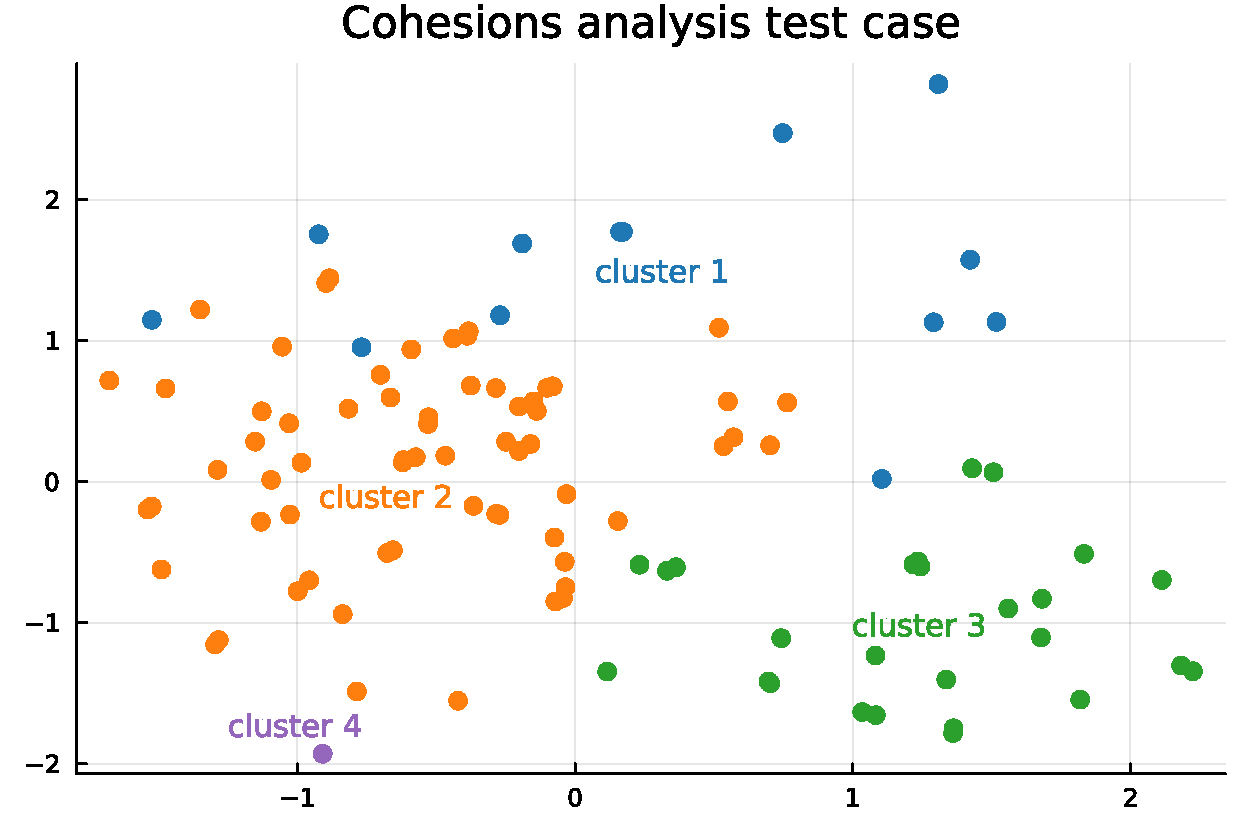
\includegraphics[width=1\linewidth]{model description/spatial cohesion analysis/cohesions_test.pdf}
    \caption[Partition considered for the cohesion analysis]{Partition considered to analyse the spatial cohesions.}
    \label{fig: cohesions_test}
\end{figure}

The first cohesion uses a tessellation idea from \cite{cohesion1-denison} that considers $\mathcal{D}_h = \sum_{i \in S_h} \| \vec{s}_i - \vec{\bar s}_h\|$ as the total distance from the units to the cluster centroid $\vec{\bar s}_h$. The computation is then an adjustment of a decreasing function in terms of $\mathcal{D}_h$, to give an higher weight on clusters which are denser, i.e. that have lower $\mathcal{D}_h$, with an additional parameter $\alpha$ to provide more control on the penalization.
\begin{equation}    
C_1(S_{h},\vec{s}_{h}^\star) = \begin{cases}
    \dfrac{M \cdot \Gamma(|S_h|)}{\Gamma(\alpha \mathcal{D}_h) \indicator{[\mathcal{D}_h\geq 1]} + \mathcal{D}_h \indicator{[\mathcal{D}_h<1]}} & \text{if } |S_h| > 1\\ 
   \hfil M & \text{if } |S_h| = 1
\end{cases}
\end{equation}

The second function provides, instead, a hard cluster boundary, where the weight is set to 1, i.e. 0 with the logarithm view, only if all the distances between all possible pairs of points inside the cluster are below the threshold parameter, i.e. if all units are "close enough" to each other. If this does not happen, even for a single pair of points, the returned value is 0, which corresponds to the maximum penalization since it would be $-\infty$ in the logarithm perspective. The strictness of this requirement can be adjusted trough the parameter $a$.
\begin{equation}    
C_2(S_{h},\vec{s}_{h}^\star) = M \cdot \Gamma(|S_h|) \cdot \prod_{i,j \in S_h} \indicator{[\| \vec{s}_i - \vec{s}_j \| \leq a]}
\end{equation}
According to this function, from Figure \ref{fig: cohesions 123} we can see how the purple cluster is considered the one with the highest cohesion, being a singleton. The runner-up is the green cluster, because it's the first among all the non-singletons which activates cohesion 2 when we increase the parameter $a$. The orange and blue clusters, instead, appear to be less dense since they require an higher value of $a$ to "pass" the distance check. 
% This pattern arises also in the other cohesions, where purple, green, then orange and blue appear always in this same order. 

\begin{figure}[!p]
    % 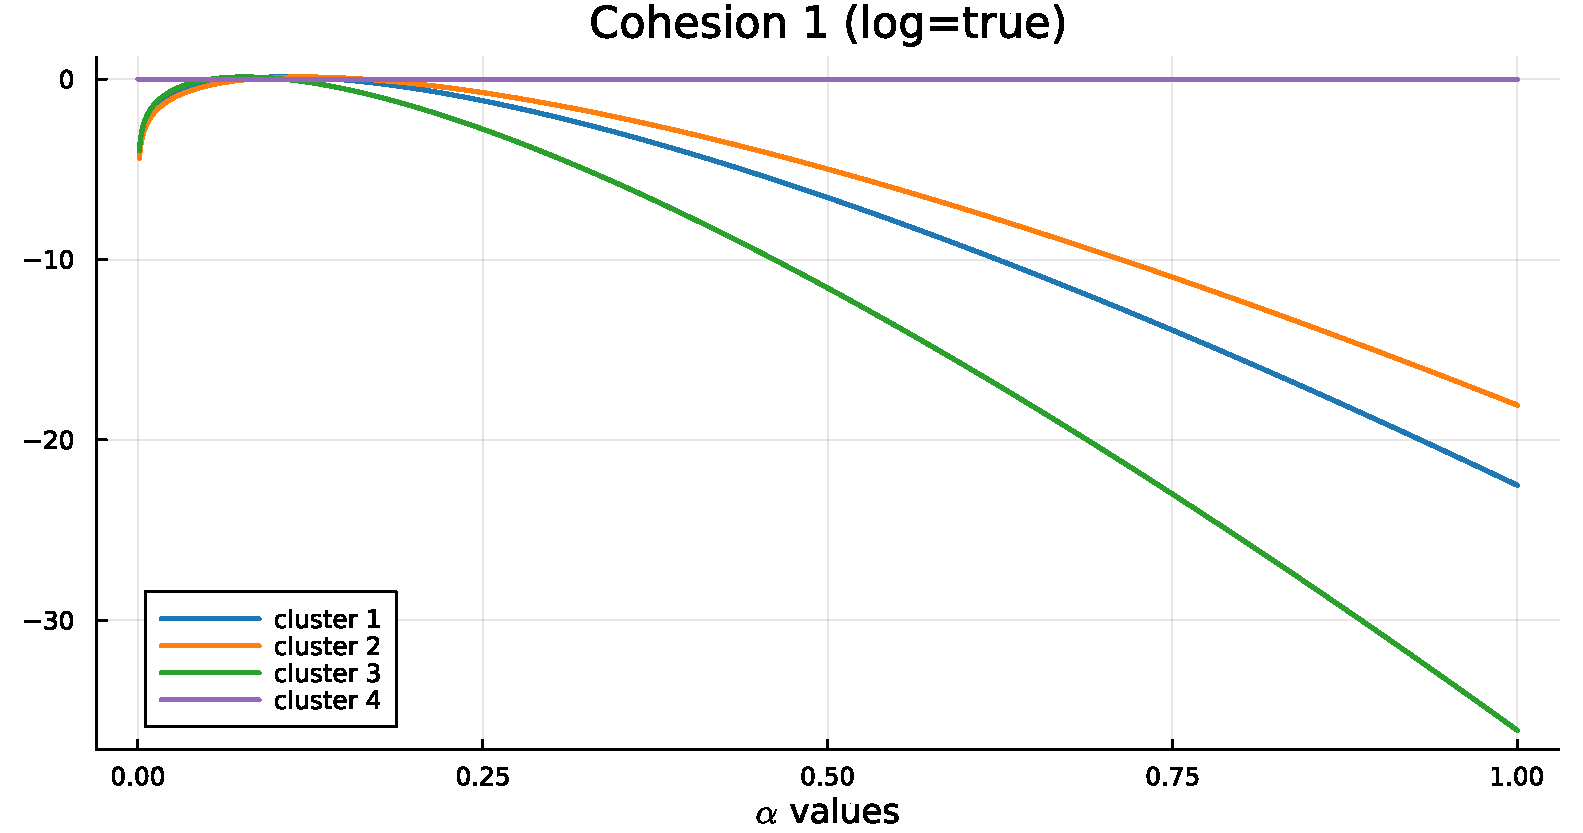
\includegraphics[width=0.5\linewidth]{model description/spatial cohesion analysis/cohesion1.pdf}
    % 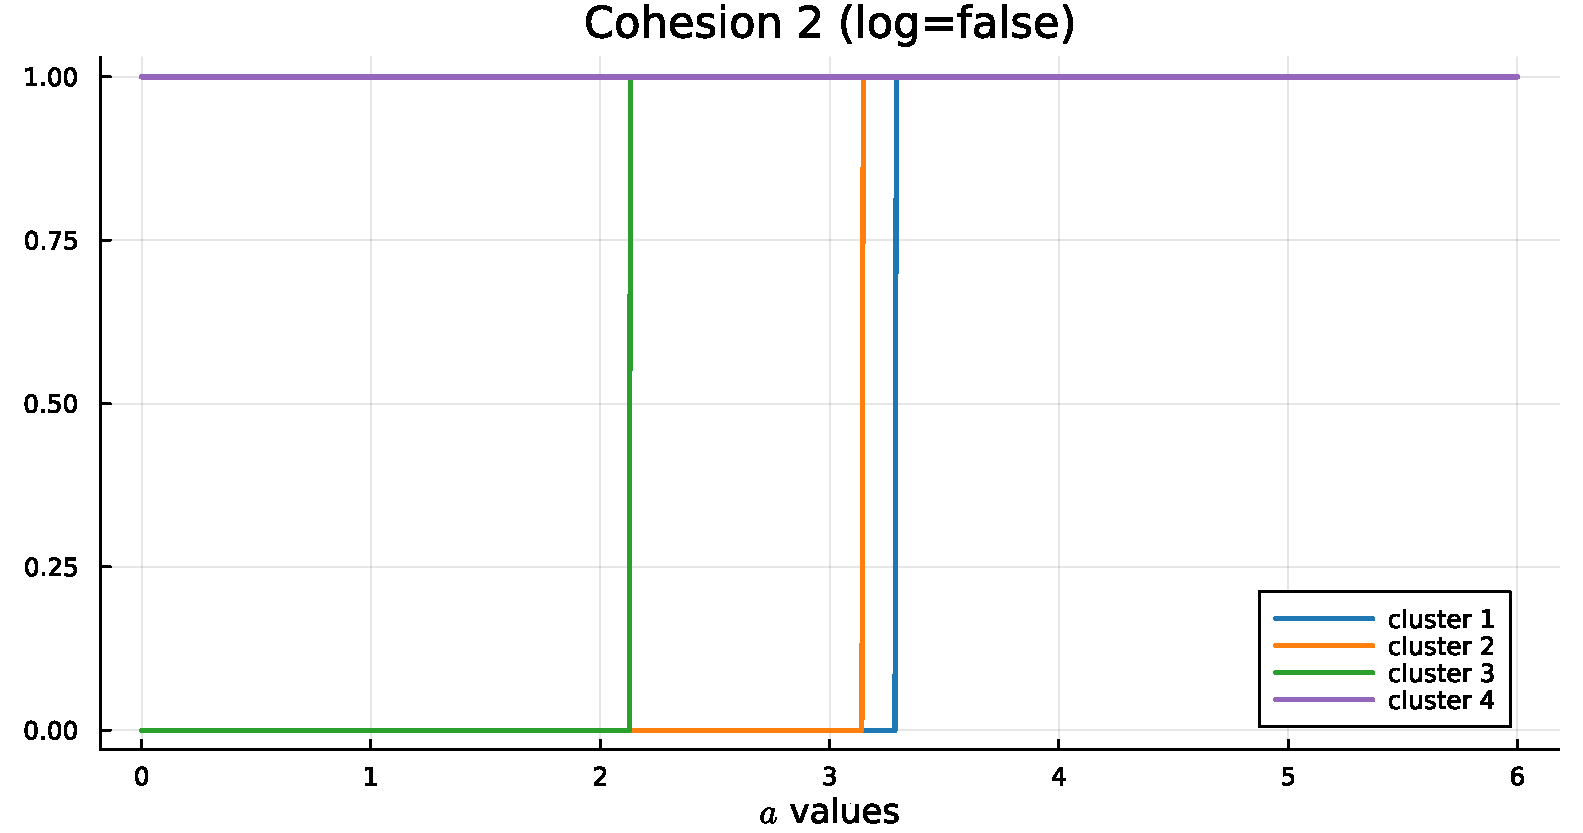
\includegraphics[width=0.5\linewidth]{model description/spatial cohesion analysis/cohesion2.pdf}\\    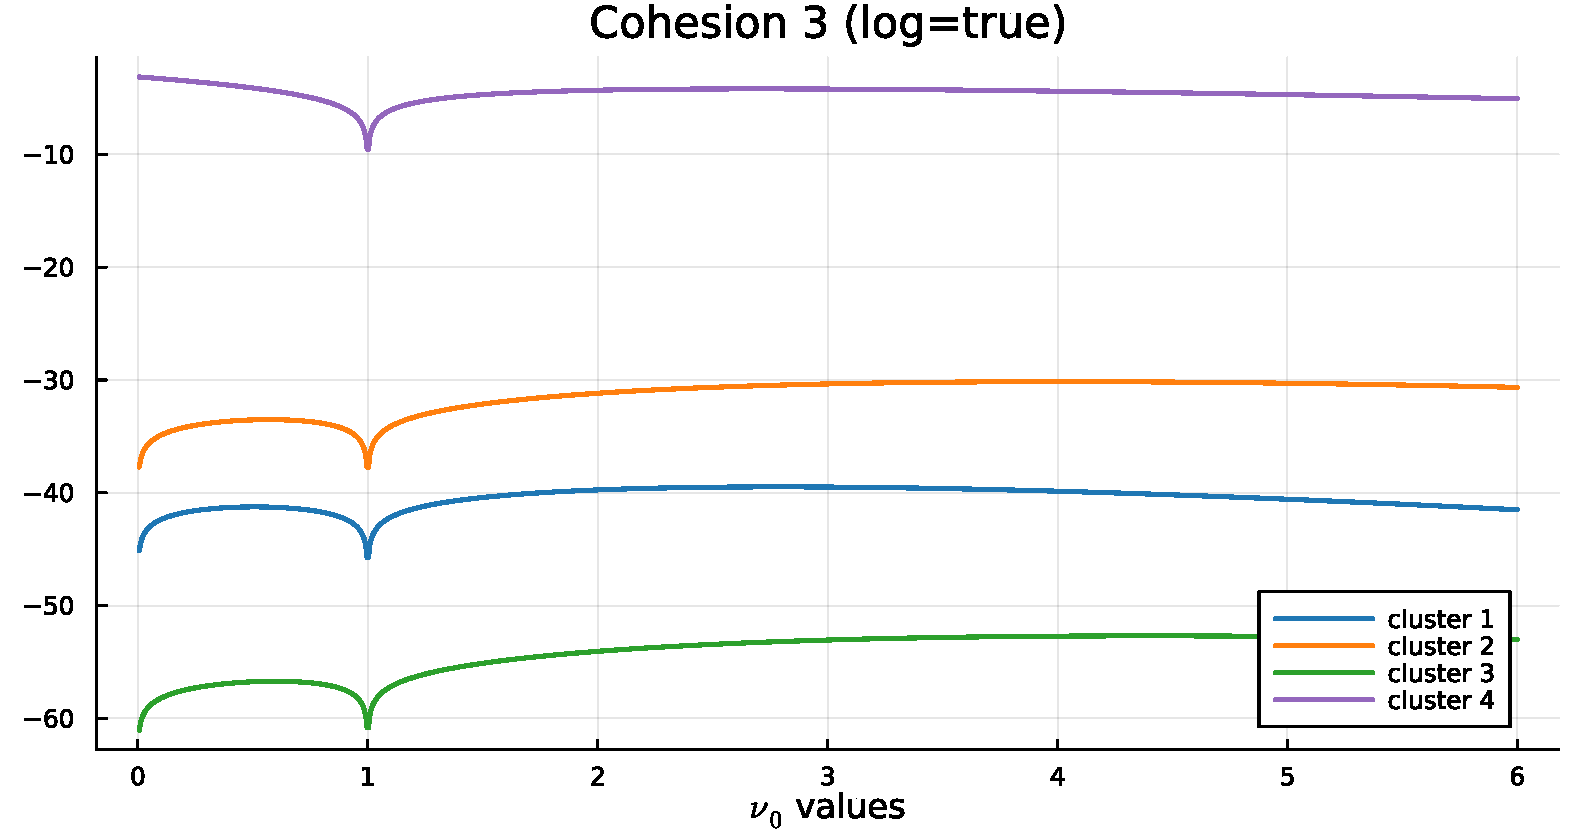
\includegraphics[width=0.5\linewidth]{model description/spatial cohesion analysis/cohesion3.pdf}
    % 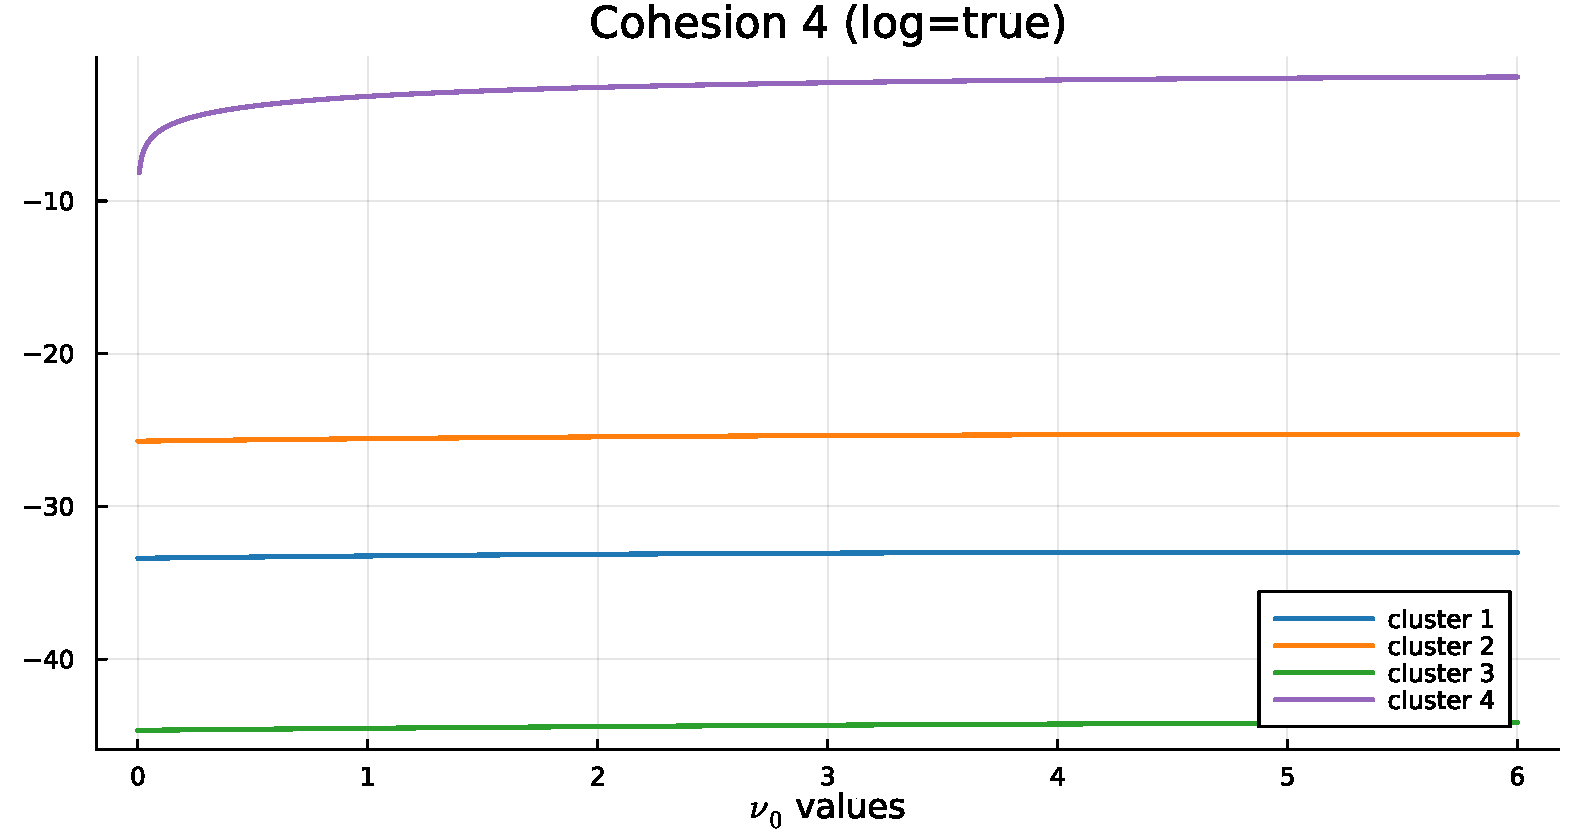
\includegraphics[width=0.5\linewidth]{model description/spatial cohesion analysis/cohesion4.pdf}\\
    % 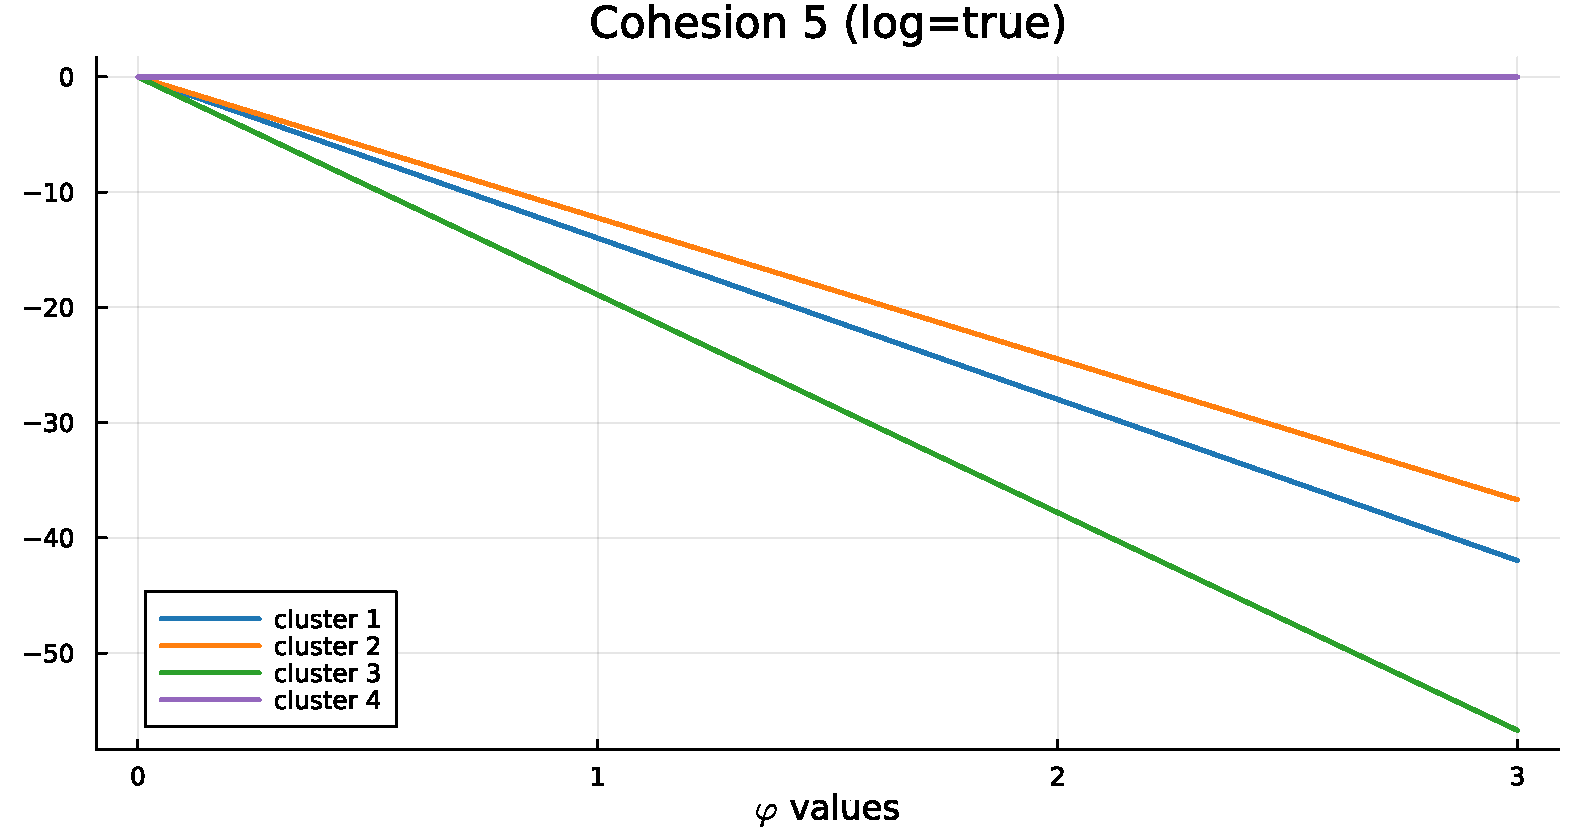
\includegraphics[width=0.5\linewidth]{model description/spatial cohesion analysis/cohesion5.pdf}
    % 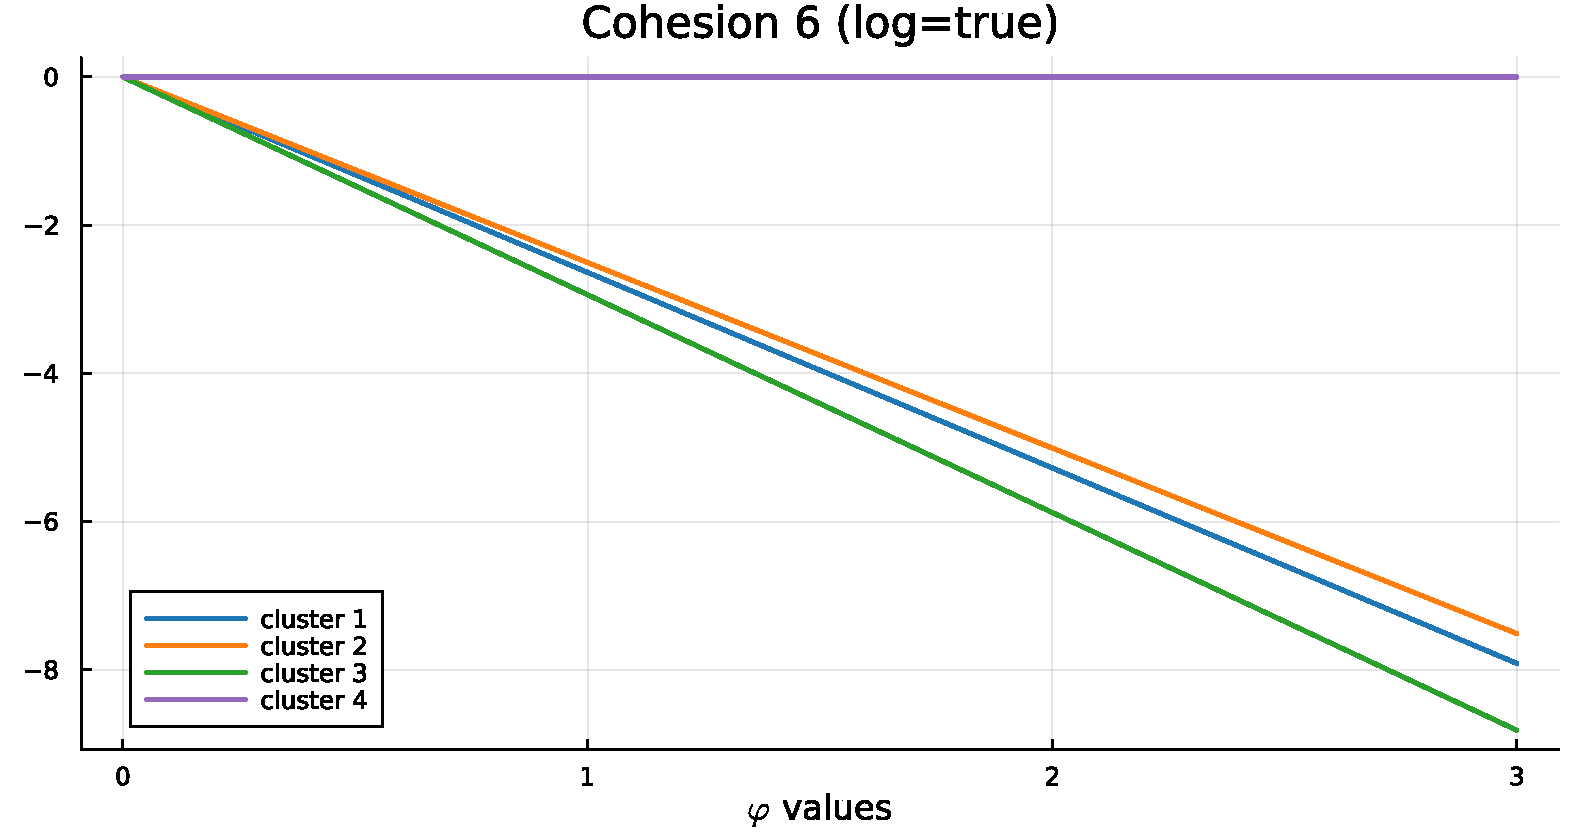
\includegraphics[width=0.5\linewidth]{model description/spatial cohesion analysis/cohesion6.pdf}\\
\centering
    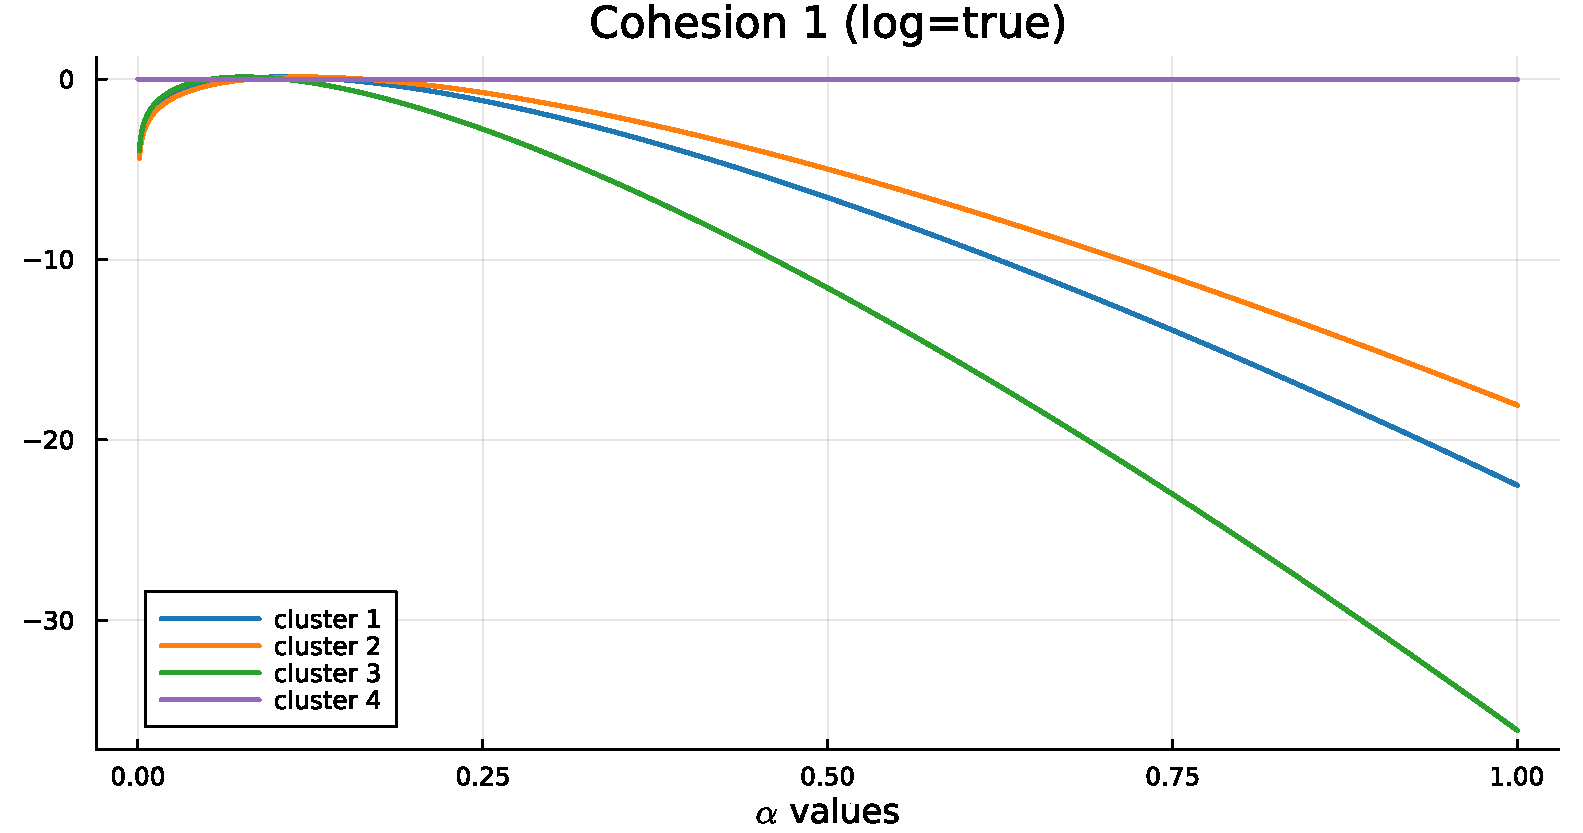
\includegraphics[width=1\linewidth]{model description/spatial cohesion analysis/cohesion1.pdf}\\
    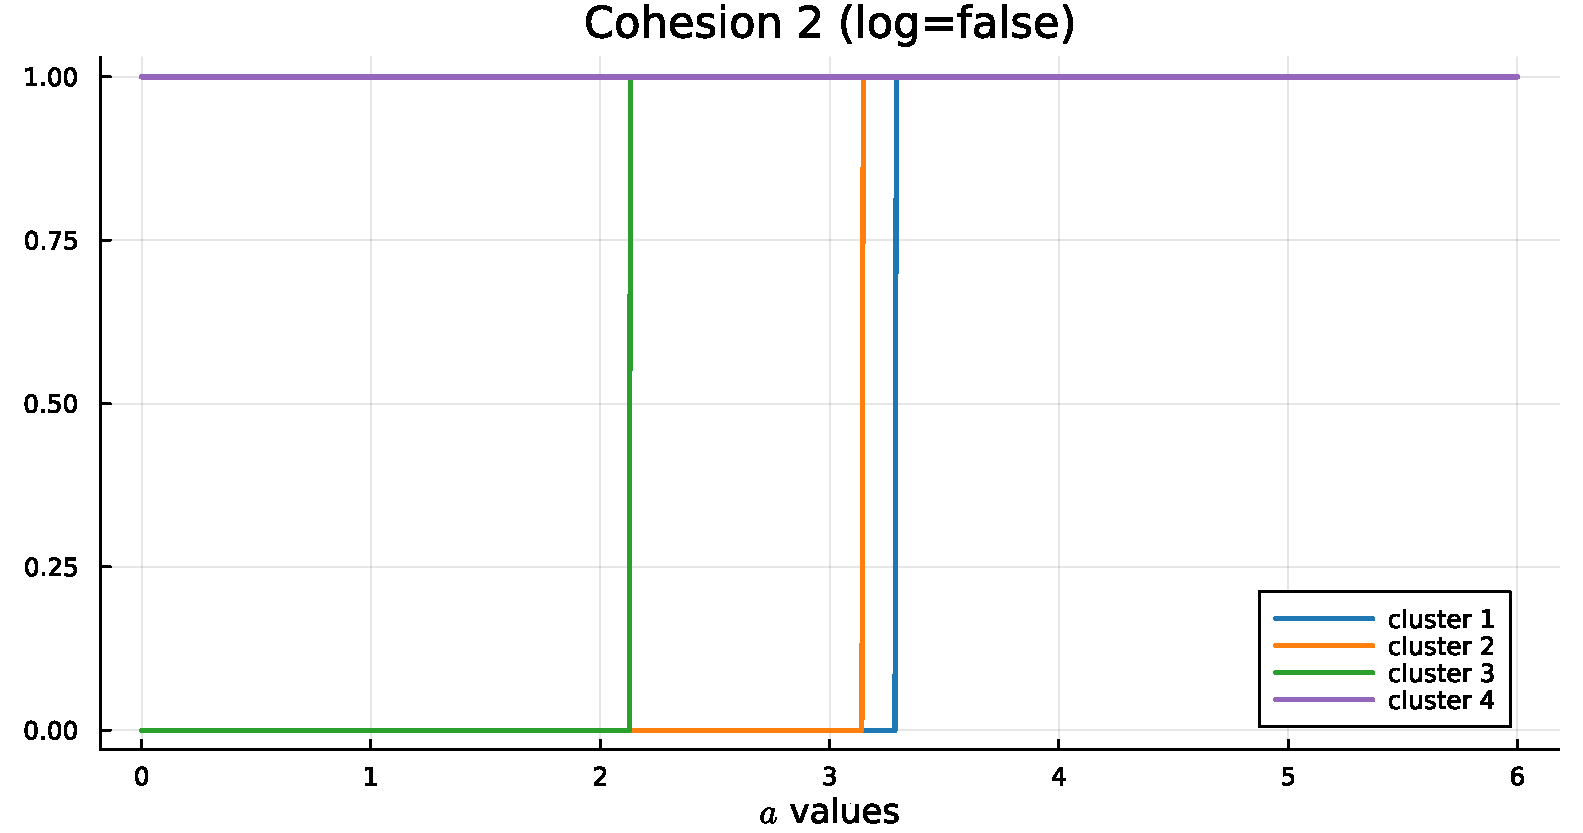
\includegraphics[width=1\linewidth]{model description/spatial cohesion analysis/cohesion2.pdf}\\
    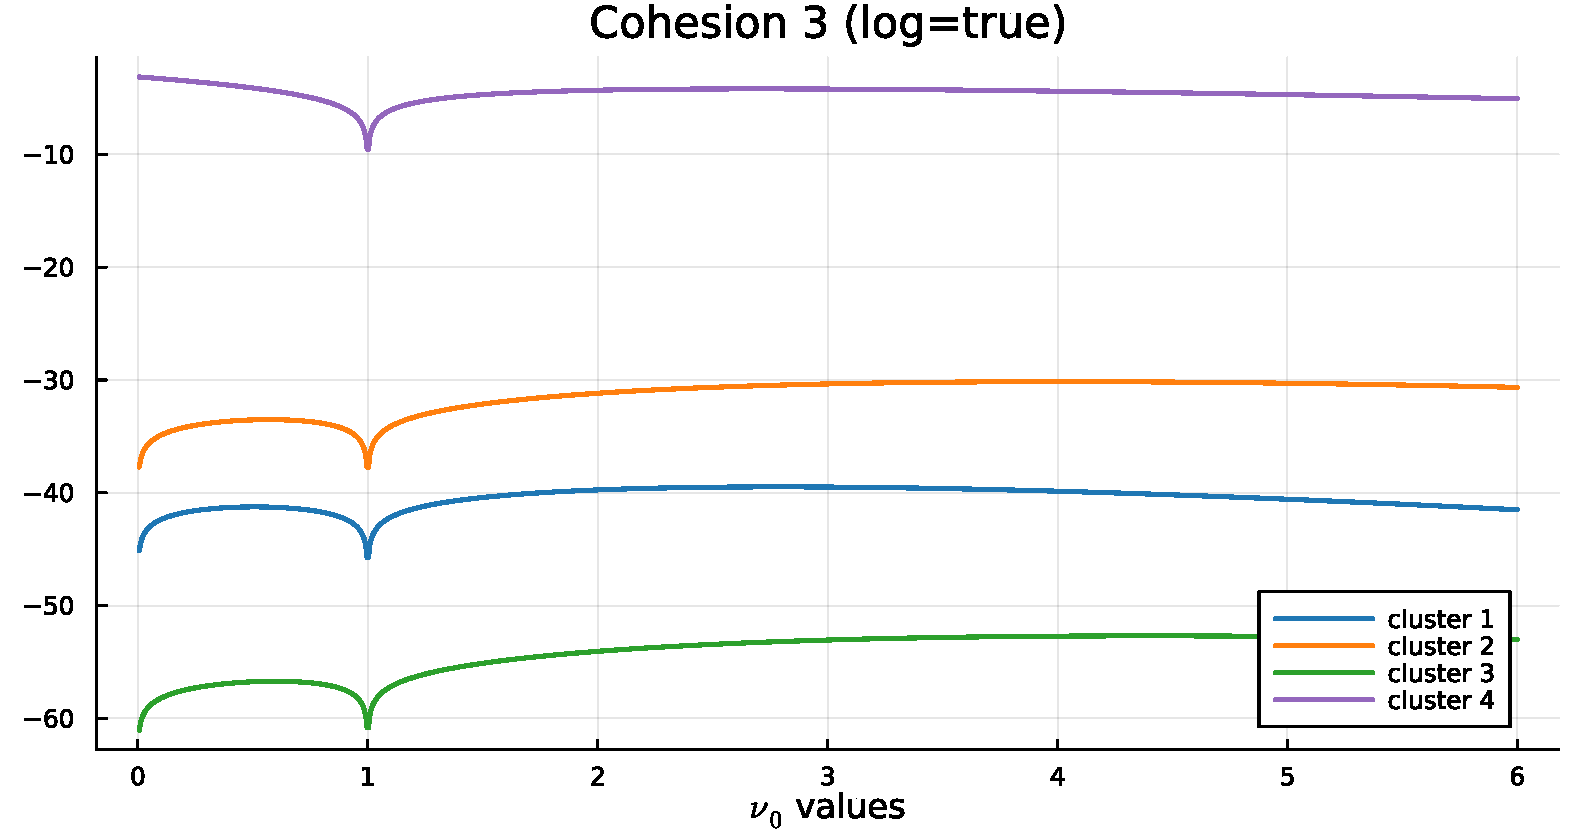
\includegraphics[width=1\linewidth]{model description/spatial cohesion analysis/cohesion3.pdf}
    \caption[Cohesions 1, 2, and 3 illustration]{Cohesions 1, 2, and 3 computed on the test case partition, with respect to different values of their tuning parameter. Cohesion 2 is without the logarithm applied just for plotting purposes, since otherwise the values would have been $-\infty$ and $0$.}
    \label{fig: cohesions 123}
\end{figure}


\begin{figure}[!p]
    % 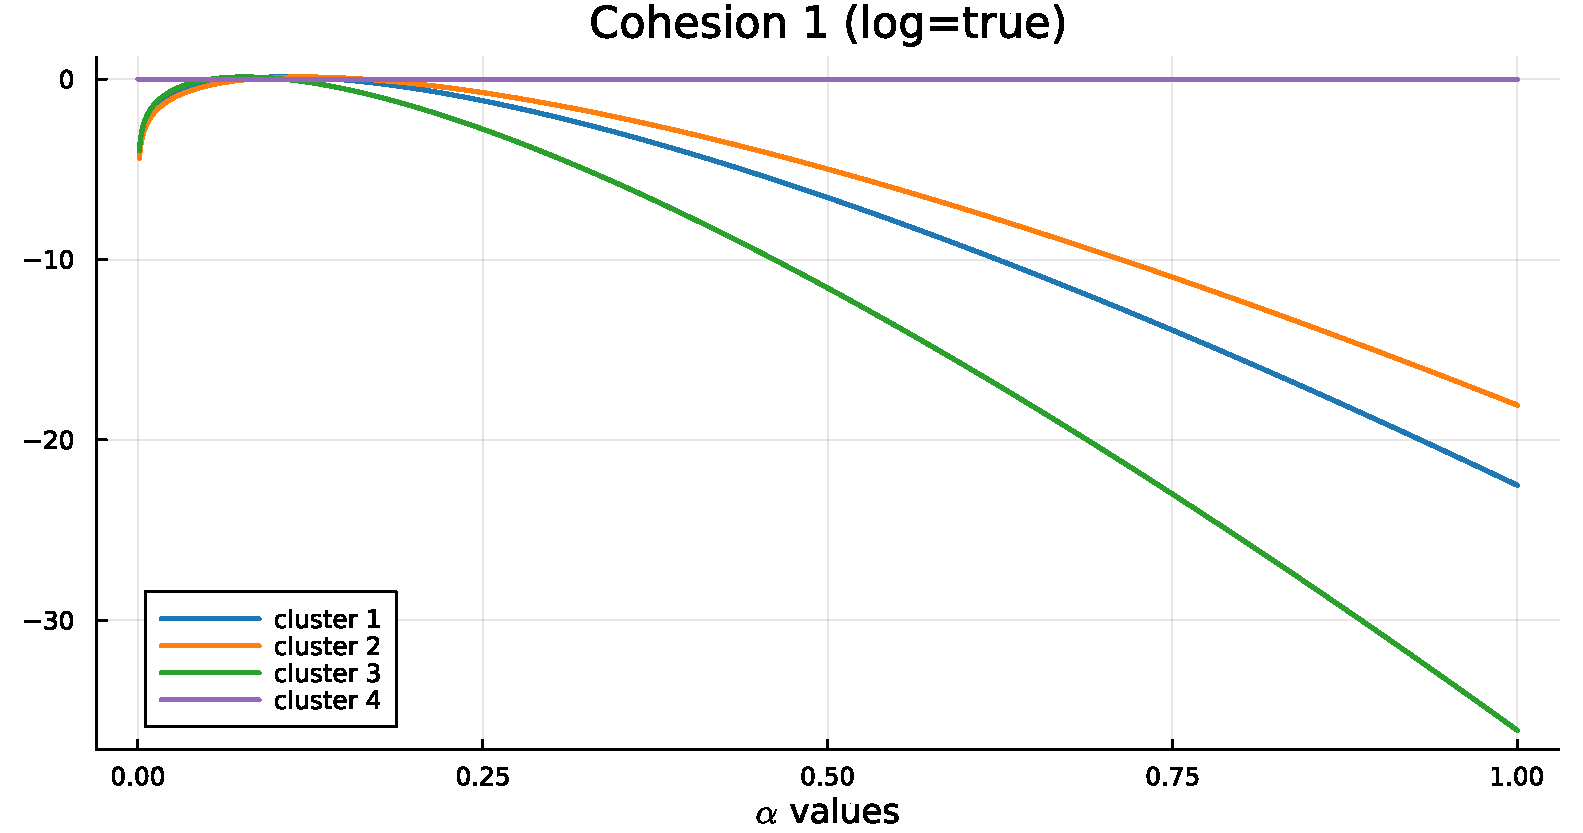
\includegraphics[width=0.5\linewidth]{model description/spatial cohesion analysis/cohesion1.pdf}
    % 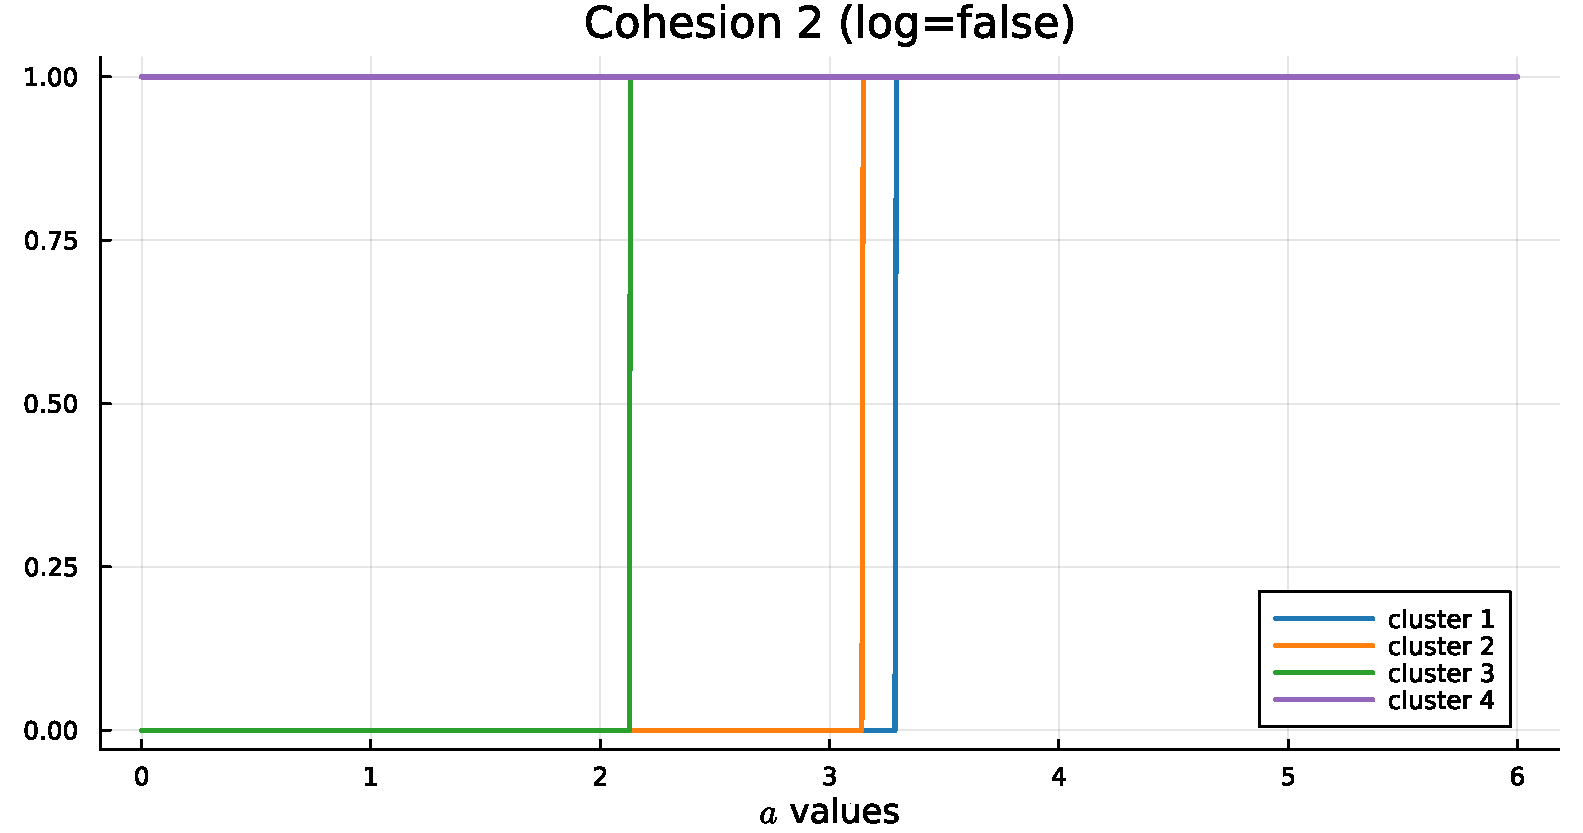
\includegraphics[width=0.5\linewidth]{model description/spatial cohesion analysis/cohesion2.pdf}\\    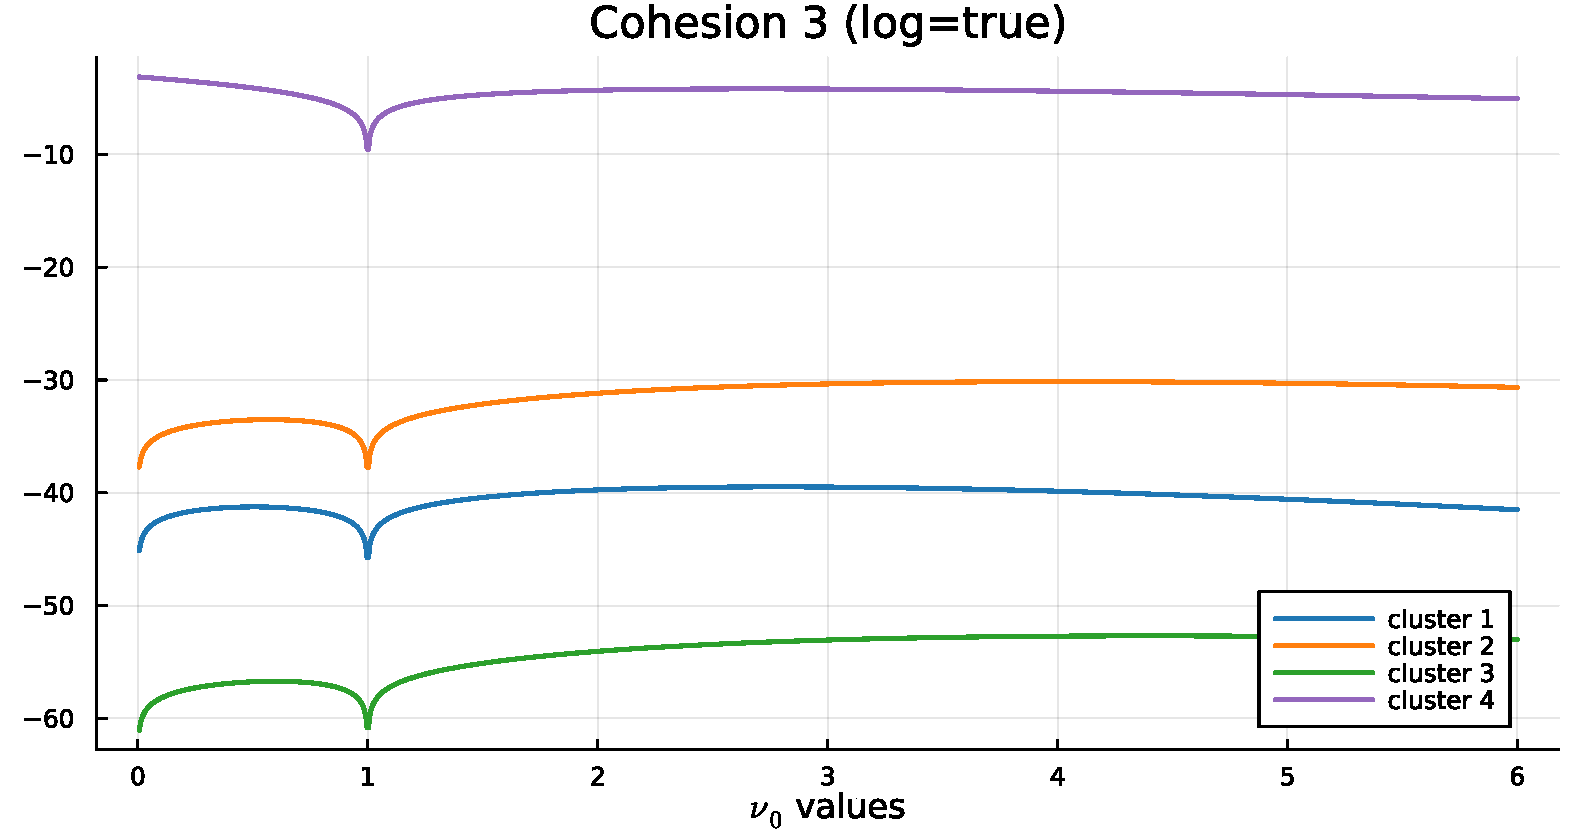
\includegraphics[width=0.5\linewidth]{model description/spatial cohesion analysis/cohesion3.pdf}
    % 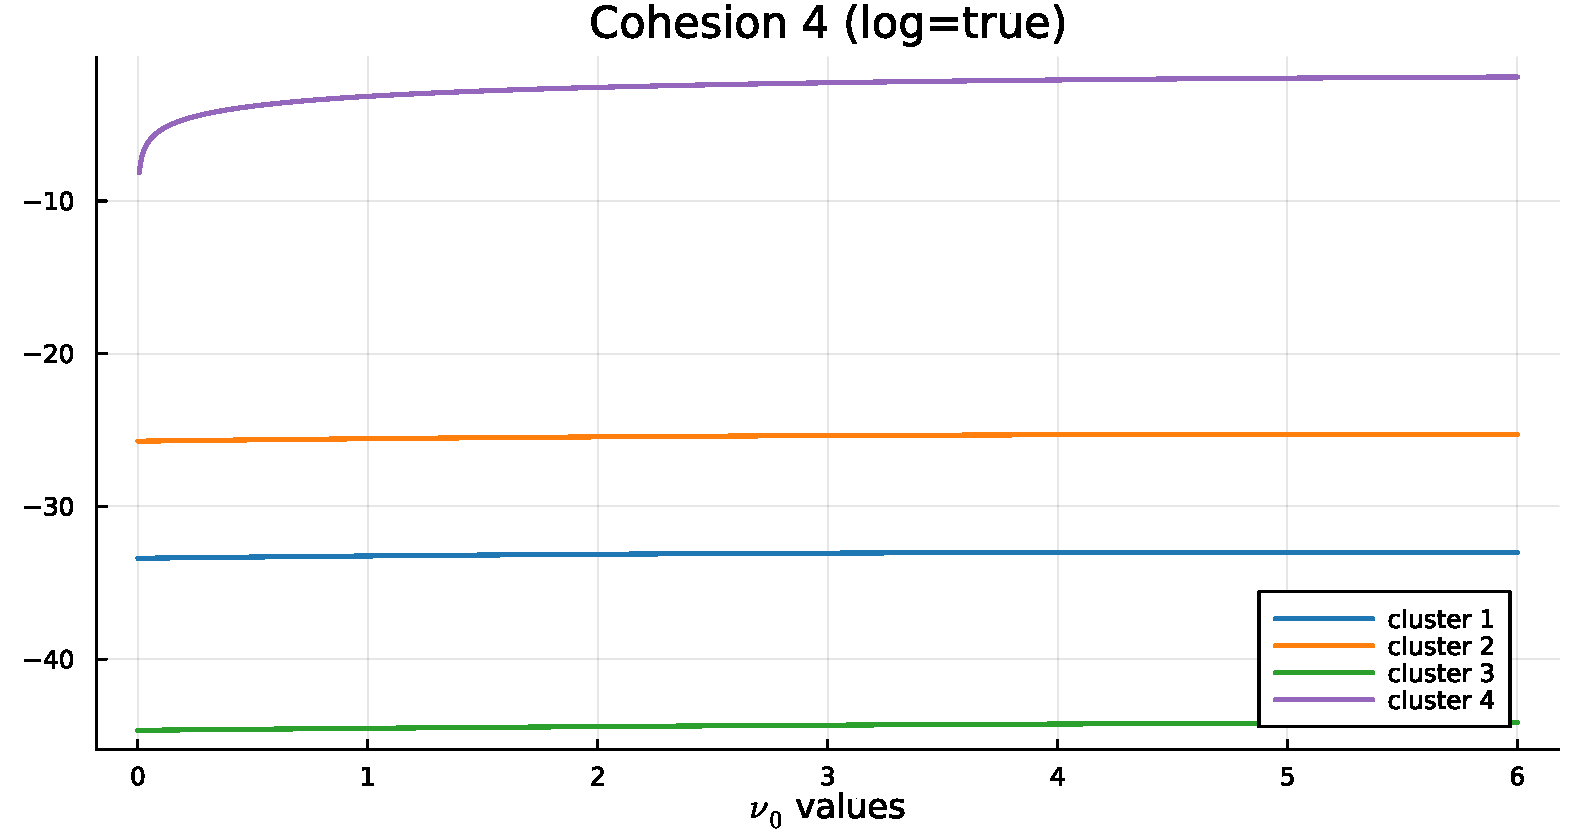
\includegraphics[width=0.5\linewidth]{model description/spatial cohesion analysis/cohesion4.pdf}\\
    % 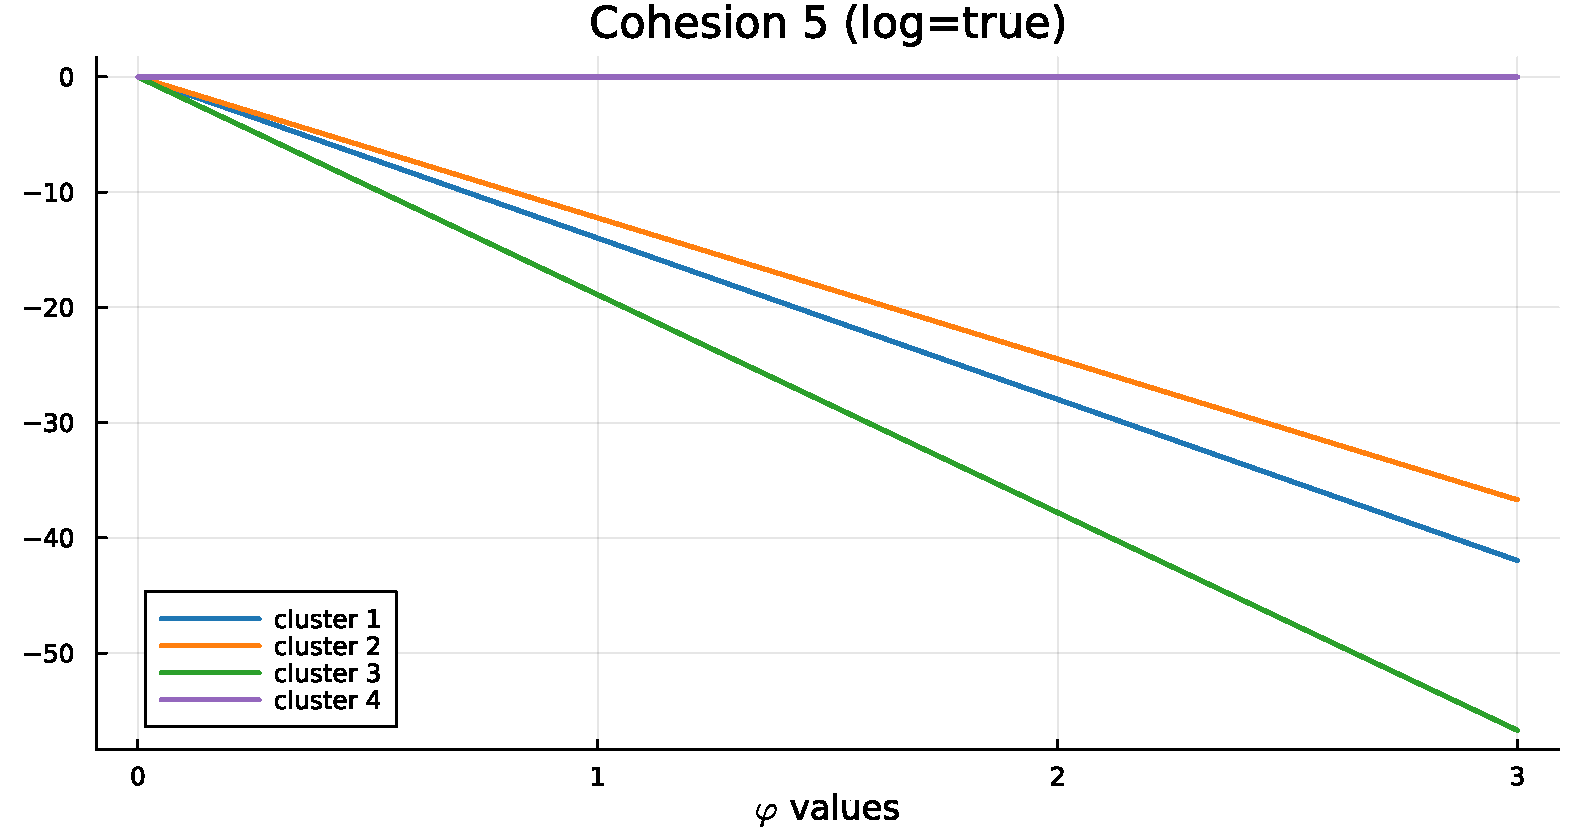
\includegraphics[width=0.5\linewidth]{model description/spatial cohesion analysis/cohesion5.pdf}
    % 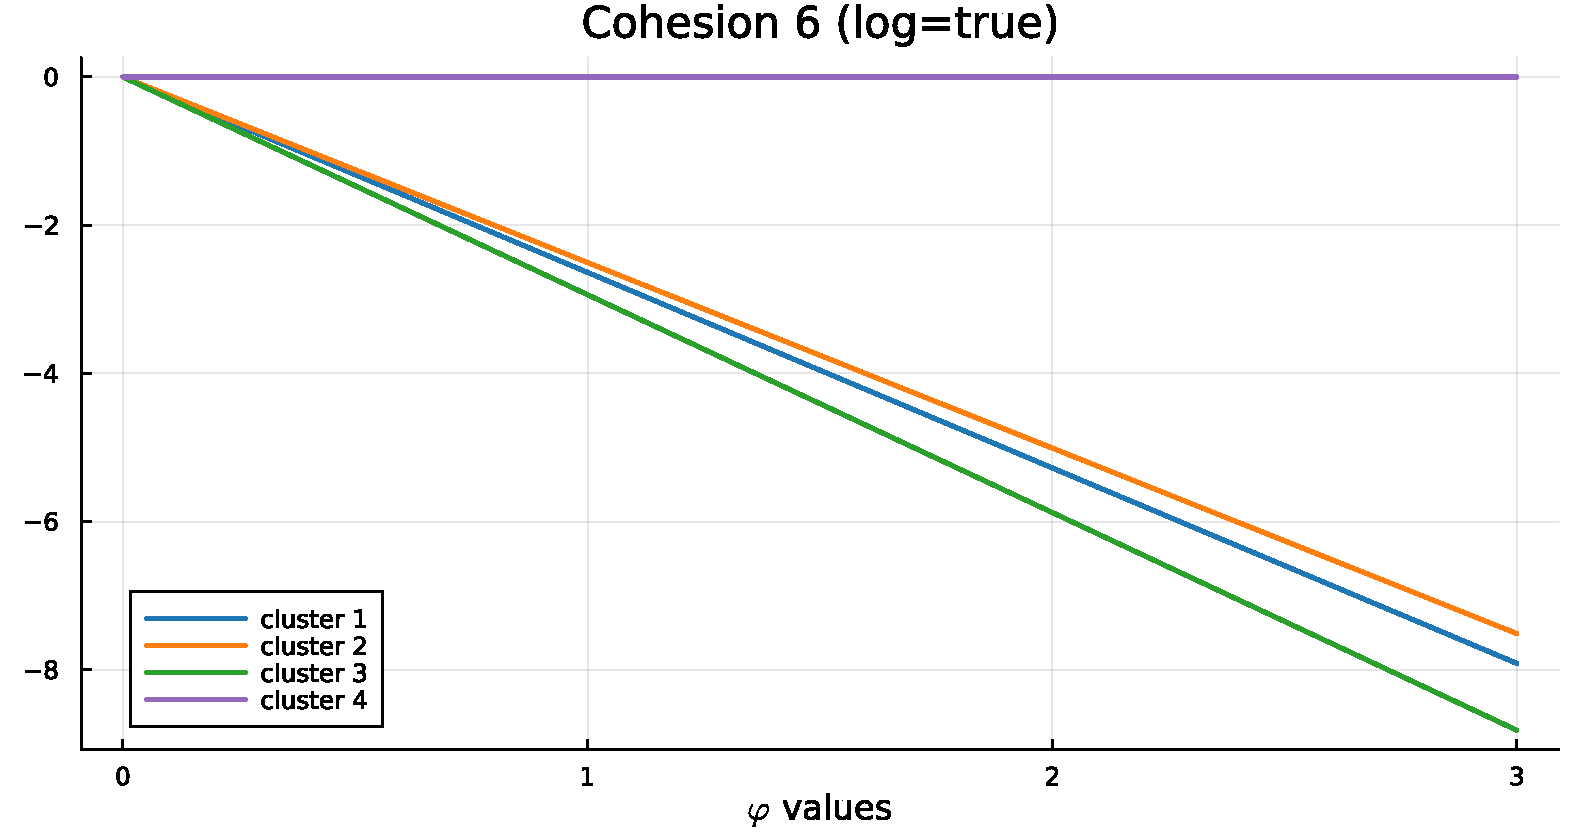
\includegraphics[width=0.5\linewidth]{model description/spatial cohesion analysis/cohesion6.pdf}\\
\centering
    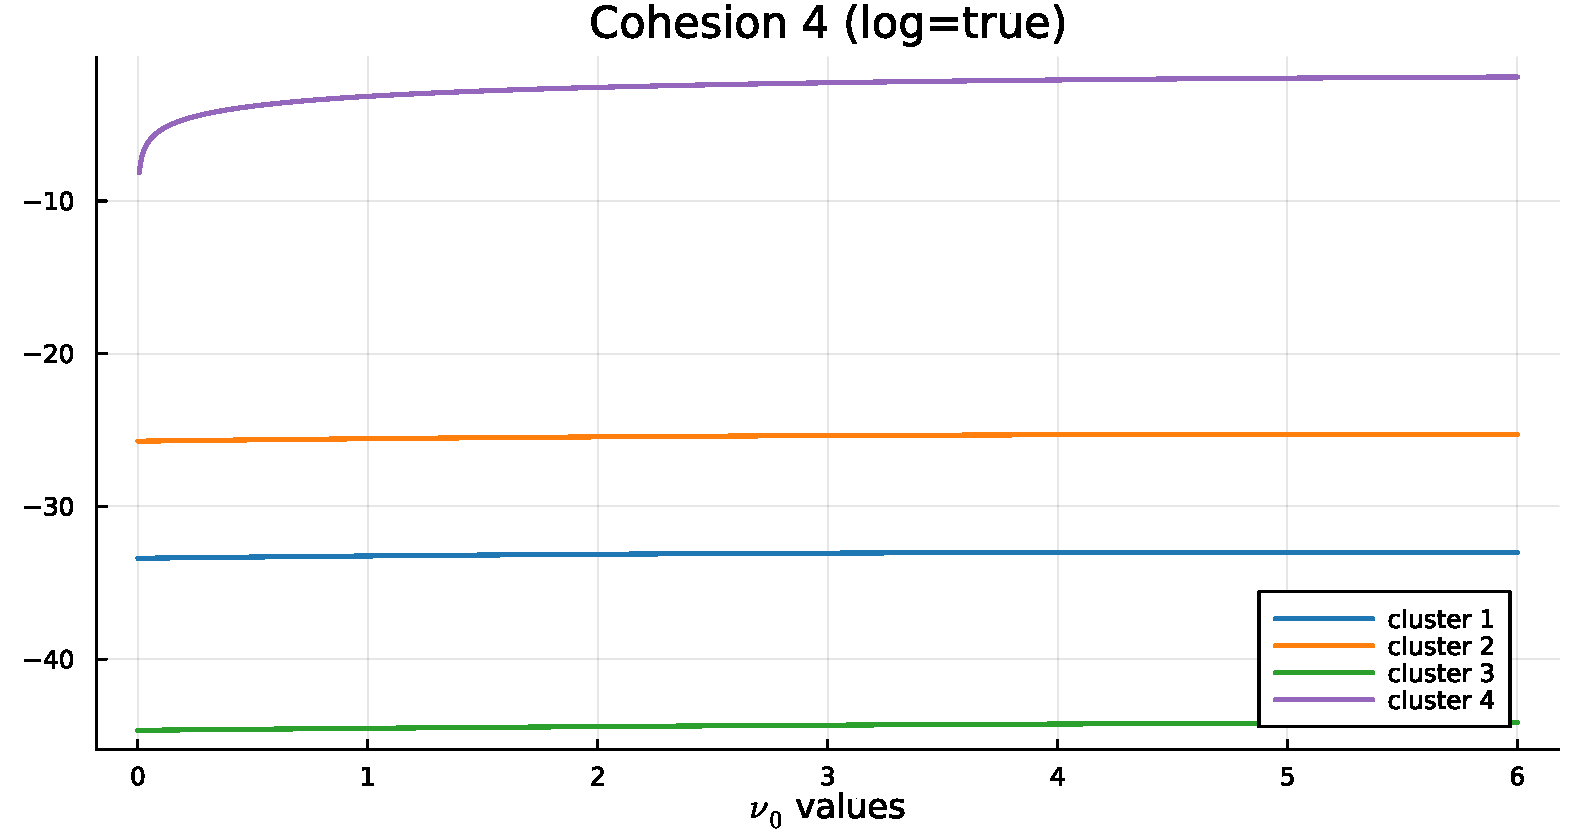
\includegraphics[width=1\linewidth]{model description/spatial cohesion analysis/cohesion4.pdf}\\
    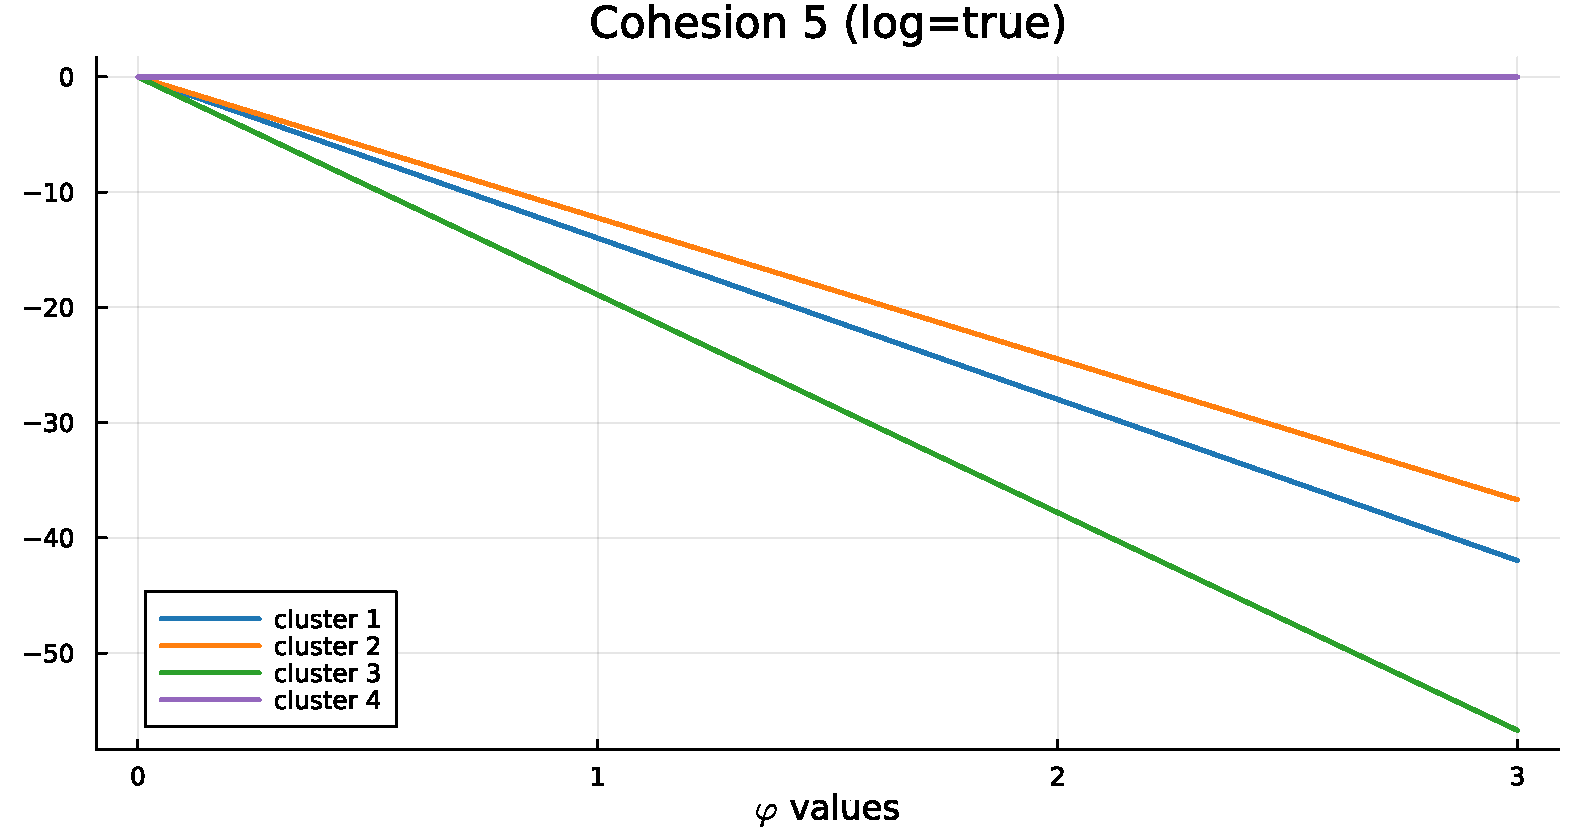
\includegraphics[width=1\linewidth]{model description/spatial cohesion analysis/cohesion5.pdf}\\
    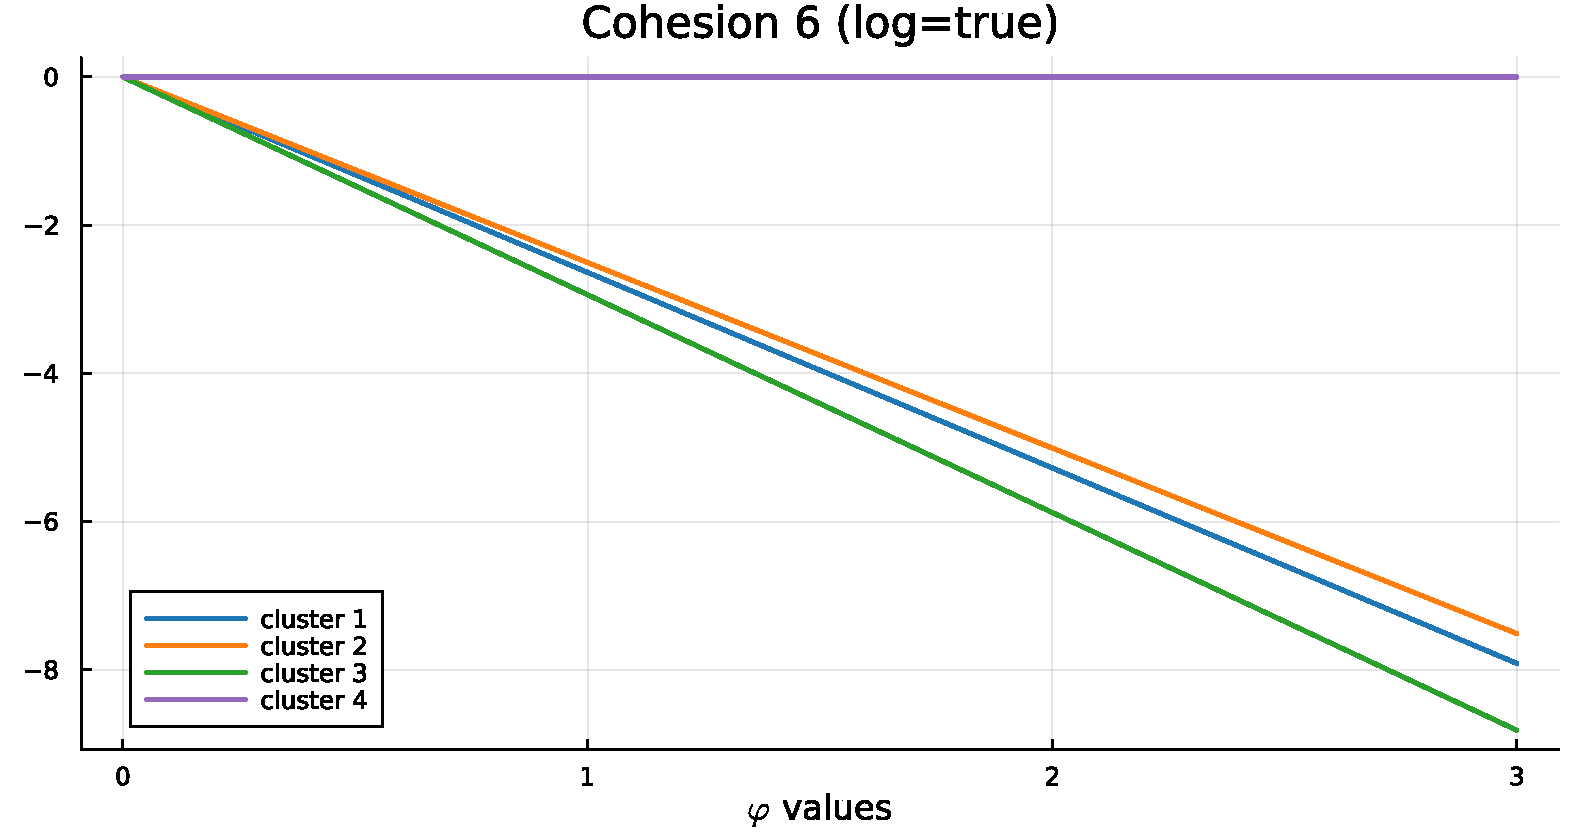
\includegraphics[width=1\linewidth]{model description/spatial cohesion analysis/cohesion6.pdf}
    \caption[Cohesions 4, 5, and 6 illustration]{Cohesions 4, 5, and 6 computed on the test case partition, with respect to different values of their tuning parameter.}
    \label{fig: cohesions 456}
\end{figure}

However, cohesions $C_1$ and $C_2$ do not preserve the exchangeability property, meaning that if we would marginalize the random partition model over the last of $m$ units we would not get to the same model as if we only had $m-1$ units. This coherence property, known as sample size consistency or addition rule \cite{sample-size-consistency}, is instead often desirable, for theoretical or computational purposes, and the following two cohesions are able to provide it \cite{paper2}.

Cohesion 3, called auxiliary similarity, treats the spatial coordinates $\vec{s}^\star$ as if they were random, applying on them a model such as the Normal/Normal-Inverse-Wishart with $\vec{\csi} = (\vec{m},V)$, $\vec{s}|\vec{\csi} \sim \N(\vec{m},V)$ and $\vec{\csi} \sim \mathcal{NIW}( \vec{\mu}_0,\kappa_0, \nu_0, \Lambda_0)$. The idea is to assign a larger weight on clusters which produce large marginal likelihood values, i.e. which according to the modelling are more probable to appear.
% $q(\vec{s}|\vec{\csi}) = \law_{\N(\vec{\csi} = (\vec{m},V))}(\vec{s})$ and $q(\vec{\csi}) = \law_{\mathcal{NIW}(\vec{\mu}_0,\kappa_0, \nu_0, \Lambda_0)}(\vec{\csi})$.
\begin{equation}    
C_3(S_{h},\vec{s}_{h}^\star) = M \cdot \Gamma(|S_h|) \cdot \int \prod_{i \in S_h} q(\vec{s}_i|\vec{\csi}_h) q(\vec{\csi}_h) \, d\vec{\csi}_h
\end{equation}

On the same line there is cohesion 4, the double dipper cohesion \cite{double-dipper}, which now employs the posterior predictive distribution rather than the prior predictive distribution of cohesion $C_3$. 
\begin{equation}    
C_4(S_{h},\vec{s}_{h}^\star) = M \cdot \Gamma(|S_h|) \cdot \int \prod_{i \in S_h} q(\vec{s}_i|\vec{\csi}_h) q(\vec{\csi}_h|\vec{s}_h^\star) \, d\vec{\csi}_h
\end{equation}

Another final idea comes from the cluster variance/entropy similarity function, a very general methodology to measure the closeness of a set of values which in fact will be used also for the covariates case. As in cohesion $C_1$, the idea is to derive a summary of the closeness of the units, summing the distance of the units from the cluster centroid, and then adjust the penalization trough the parameter $\phi$, to control how much penalize dissimilar values. 
\begin{equation}    
C_5(S_{h},\vec{s}_{h}^\star) = \expp{-\phi \sum_{i \in S_h} \| \vec{s}_i - \vec{\bar{s}}_h\| }
\end{equation}
\begin{equation}    
C_6(S_{h},\vec{s}_{h}^\star) = \expp{-\phi \log( \sum_{i \in S_h} \| \vec{s}_i - \vec{\bar{s}}_h\| )}
\end{equation}

\section{Covariates similarities analysis}
\label{Covariates similarity analysis}

A wide spectrum of choice is also available for covariates similarities \cite{paper6}. To account for them, the idea consists in extending the PPM to make it function of $S_{jt}$, $\vec{s}_{jt}^\star$, and now also of $X_{jt}^\star$, being this the $p \times |S_{jt}|$ matrix storing the covariates of the units belonging to cluster $j$ at time $t$, i.e. $X_{jt}^\star = \{ \vec{x}_{it}^\star = (x_{it1}, \ldots, x_{itp})^T : i \in S_{jt} \}$.

For the current implementation of JDRPM we decided to treat each covariate individually, therefore the PPM will actually be function of the set of unidimensional vectors which record the different $p$ covariates of the units inside cluster $S_{jt}$, meaning $\vec{x}_{jt1}^\star, \ldots,\vec{x}_{jtp}^\star$, of which all contributions will be considered independently one to each other. In this way, the final PPM form will be
\begin{equation}
P(\rho) \propto \prod_{h=1}^{k_t} C(S_{jt},\vec{s}_{jt}^\star) \left( \prod_{r=1}^p g(S_{jt},\vec{x}_{jtr}^\star) \right)
\end{equation}
where $\vec{x}_{jtr}^\star$ represents the vector recording the $r$-th covariate values for all the units inside cluster $S_{jt}$, i.e. row $r$ of matrix $X_{jt}^\star$. This choice is lighter from the theoretical and computational perspectives, and allows a mixture of numerical and categorical covariates without any problem. A unified and multidimensional consideration of the covariates is nonetheless possible, with proper adjustments on the similarities functions, and would have lead to a PPM of the form
\begin{equation}
P(\rho) \propto \prod_{h=1}^{k_t} C(S_{jt},\vec{s}_{jt}^\star) g(S_{jt},X_{jt}^\star)
\end{equation}

\begin{figure}[ht!]
    \centering
    % 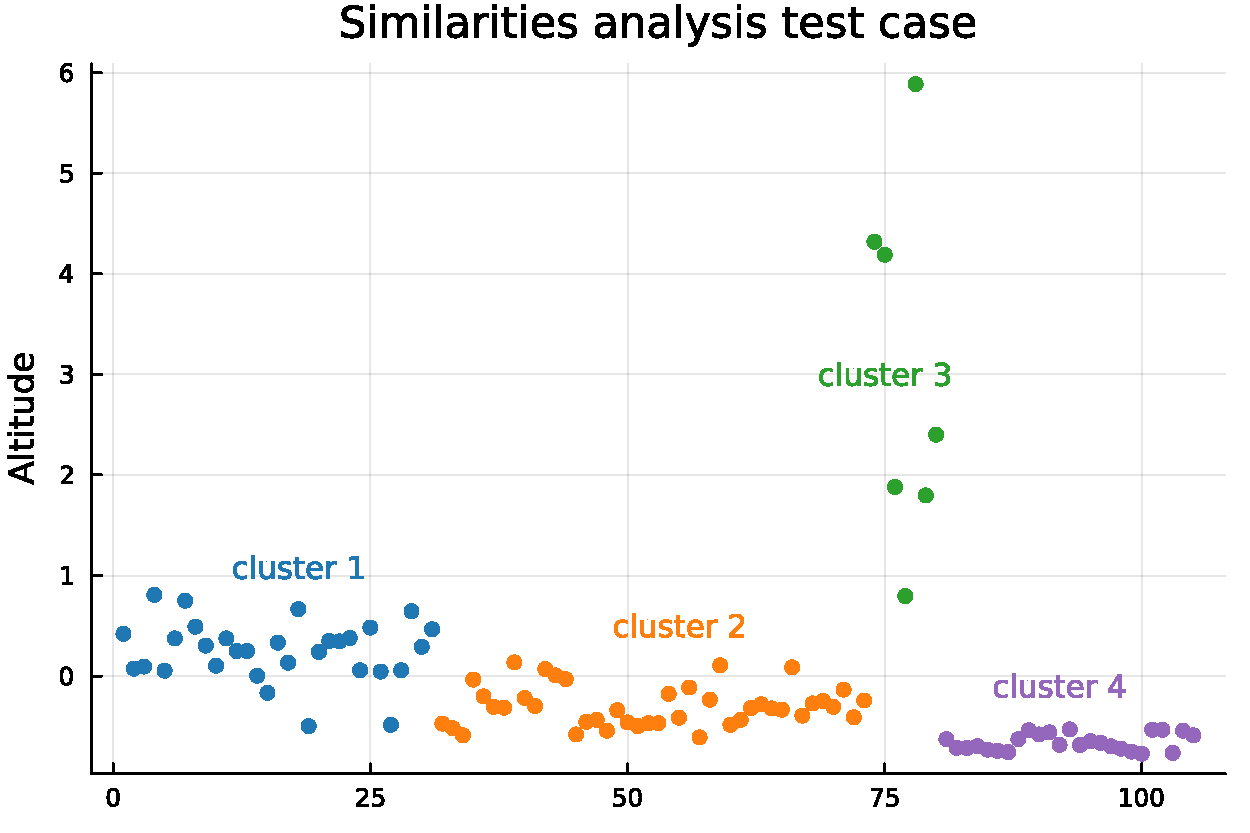
\includegraphics[width=1\linewidth]{model description/covariate similarity analysis/similarity_sorted_test.pdf}
    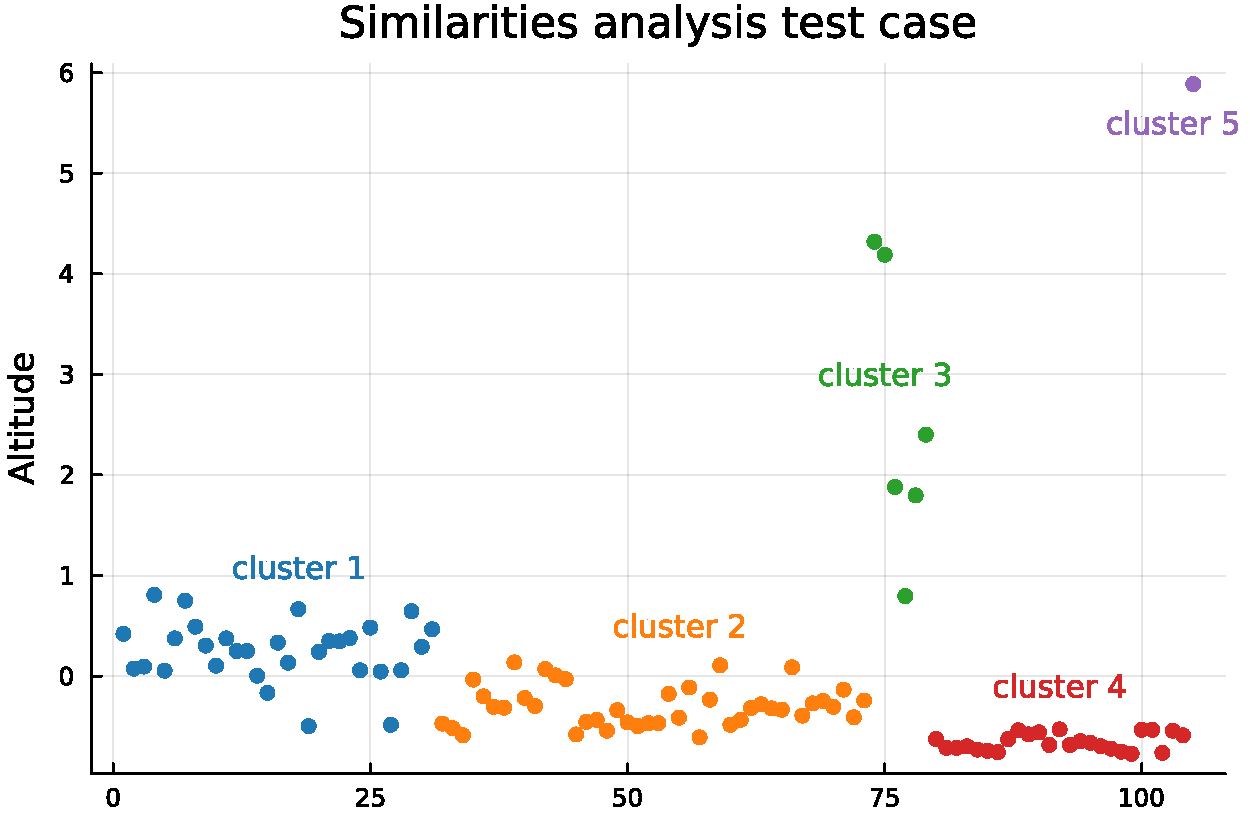
\includegraphics[width=1\linewidth]{model description/covariate similarity analysis/test case on 5 clusters/similarity_sorted_test.pdf}
    \caption[Partition considered for the similarity analysis]{Partition considered to analyse the covariate similarities. The order of the units has been modified to plot together all units belonging to the same cluster.}
    \label{fig: similarity tests}
\end{figure}


As in the previous section, we will now discuss all the similarities implemented in the JDRPM model and perform tests on each of them. All the tests will be referred to the test case partition displayed in Figure \ref{fig: similarity tests} which is about the \tt{Altitude} covariate from the spatio-temporal dataset that will be used in Chapter \ref{chap: testing}. Regarding the notation, we will again employ the simpler and general one dropping the spatio-temporal context.

The first similarity is the cluster variance/entropy similarity function, which as the name suggest can work with both numerical and categorical variables. The general form is 
\begin{equation}    
g_1(S_h,\vec{x}_{h}^\star) = \expp{-\phi H(S_h,\vec{x}_{h}^\star)}
\end{equation}
with $H(S_h,\vec{x}_{h}^\star) =  \sum_{i \in S_h} ( x_i - \bar{x}_h)^2 $ for numerical covariates, being $\bar x_h$ the mean value of the $\vec{x}_{h}^\star$ vector, and $H(S_h,\vec{x}_{h}^\star) = - \sum_{c=1}^C \hat p_c \log(\hat p_c)$ for categorical covariates, with $\hat p_c$ indicating the relative frequency at which each factor appears. The parameter $\phi$ controls the amount of penalization to apply. This function can be extended quite easily to the multidimensional case, at least for the case of numerical covariates only, where the $H$ function becomes $H(S_h,X_{h}^\star) =  \sum_{r=1}^p \| \vec{x}_{r} - \vec{\bar{x}}_h \|$.


\begin{figure}[!p]
    \centering
    % 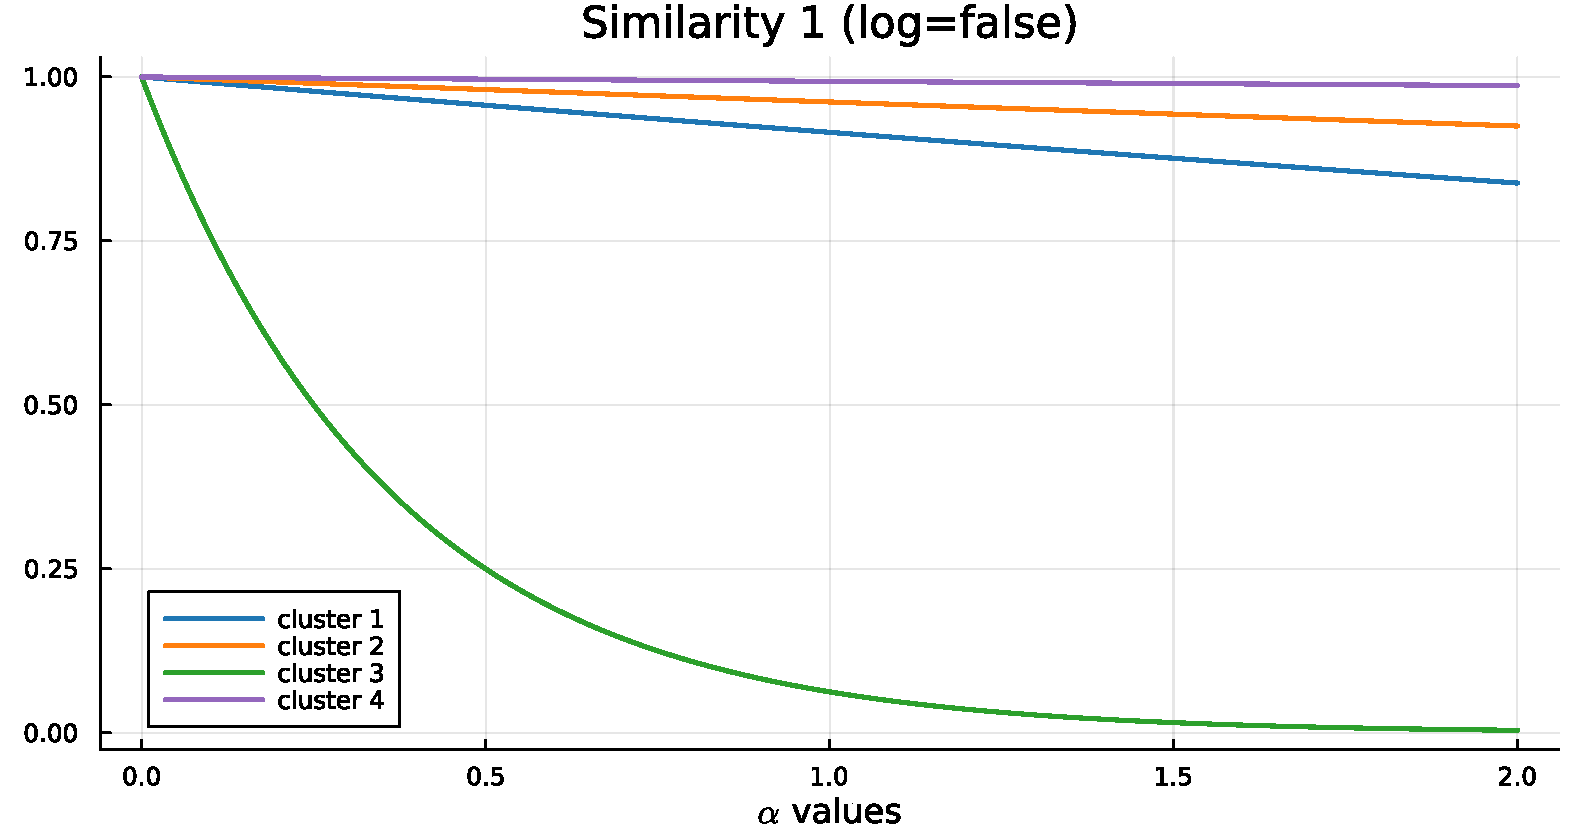
\includegraphics[width=1\linewidth]{model description/covariate similarity analysis/similarity1_log_false.pdf}
    % 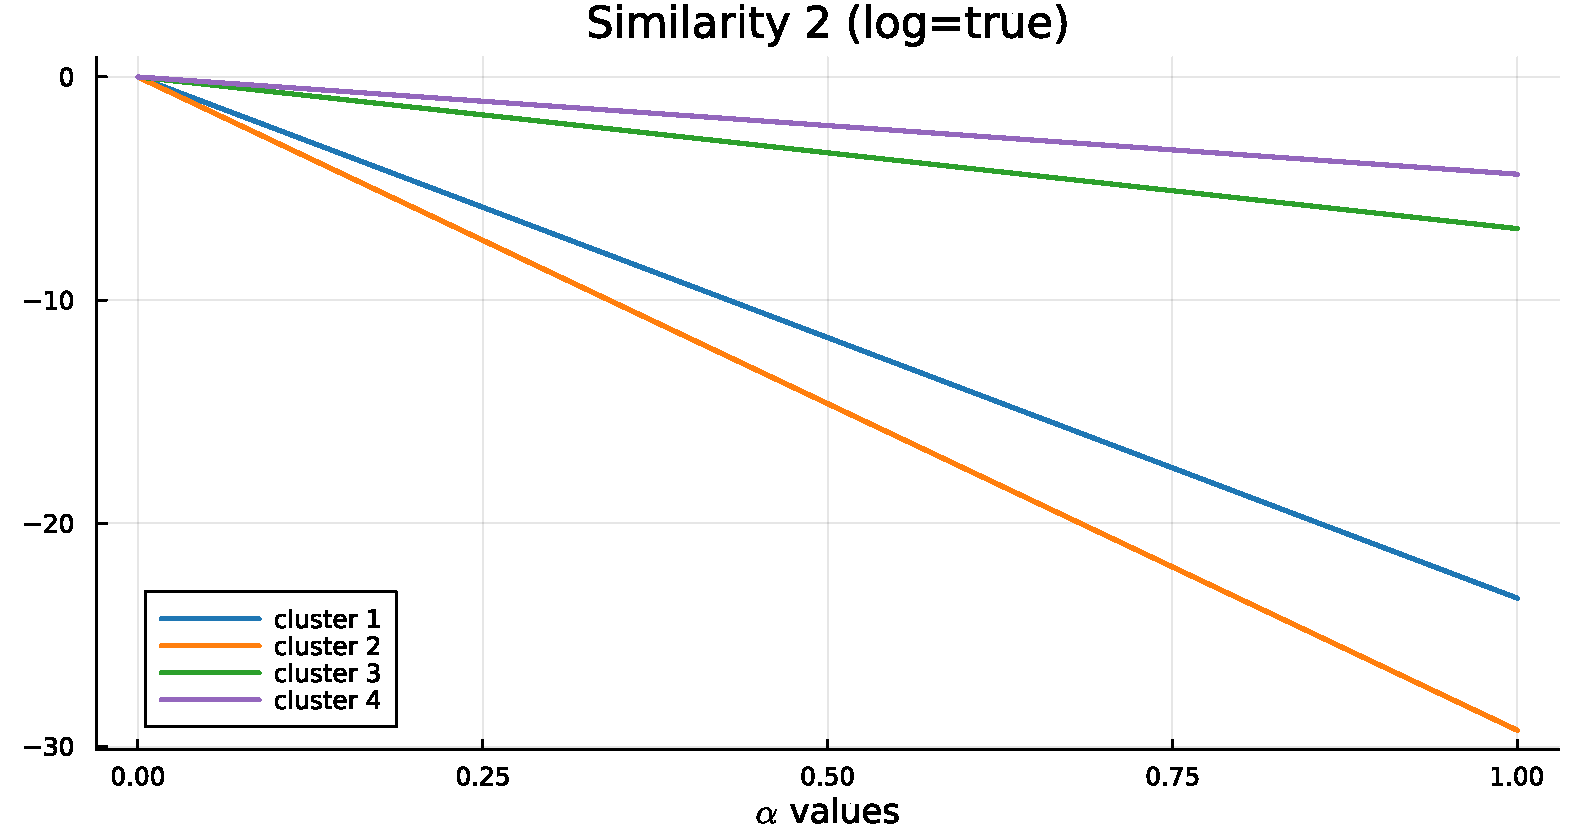
\includegraphics[width=1\linewidth]{model description/covariate similarity analysis/similarity2.pdf}
    % 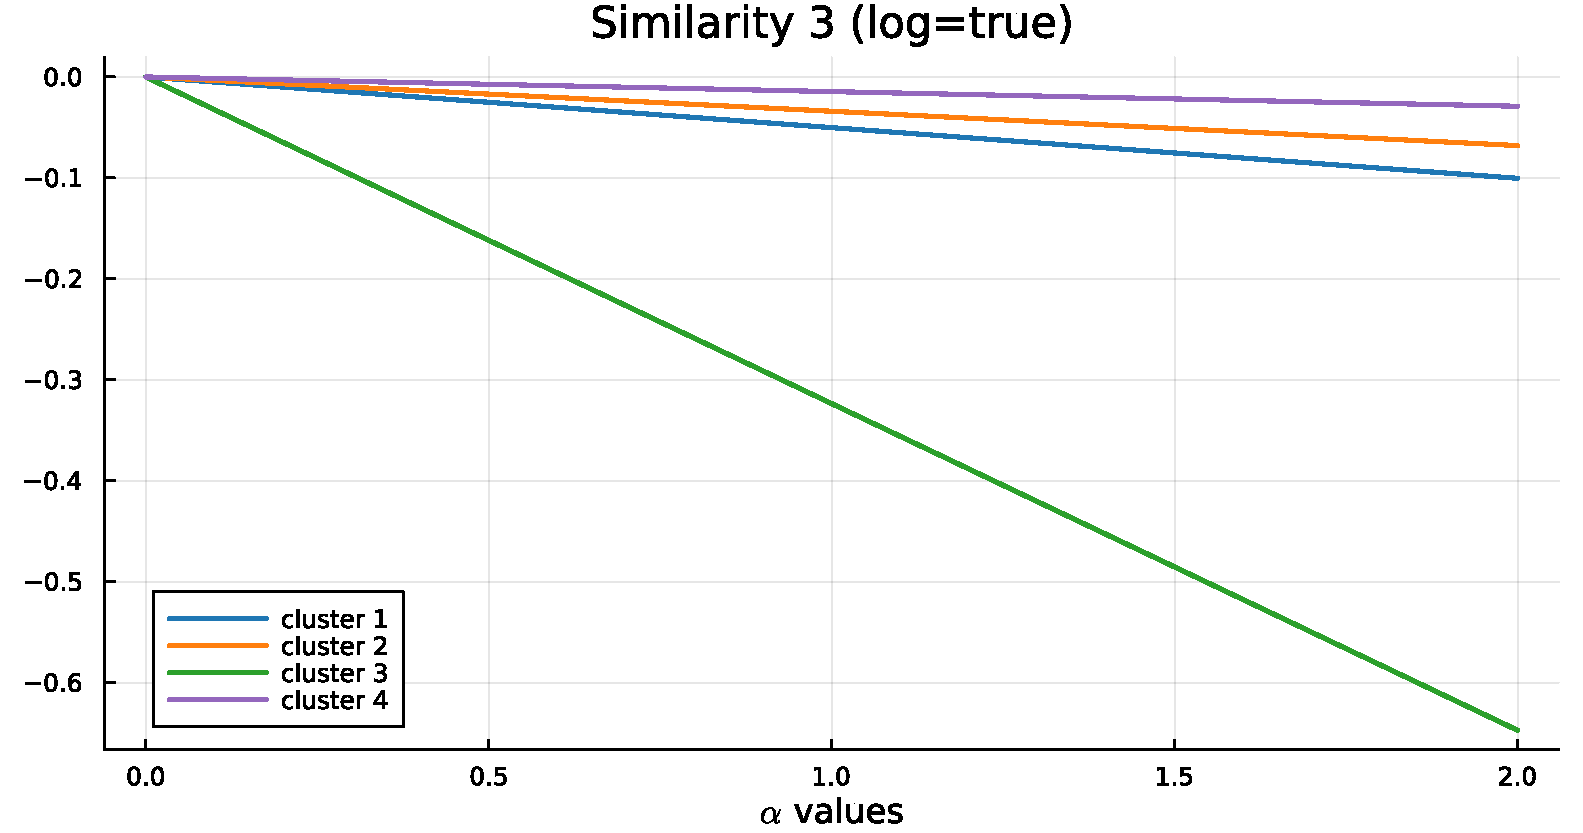
\includegraphics[width=1\linewidth]{model description/covariate similarity analysis/similarity3.pdf}
    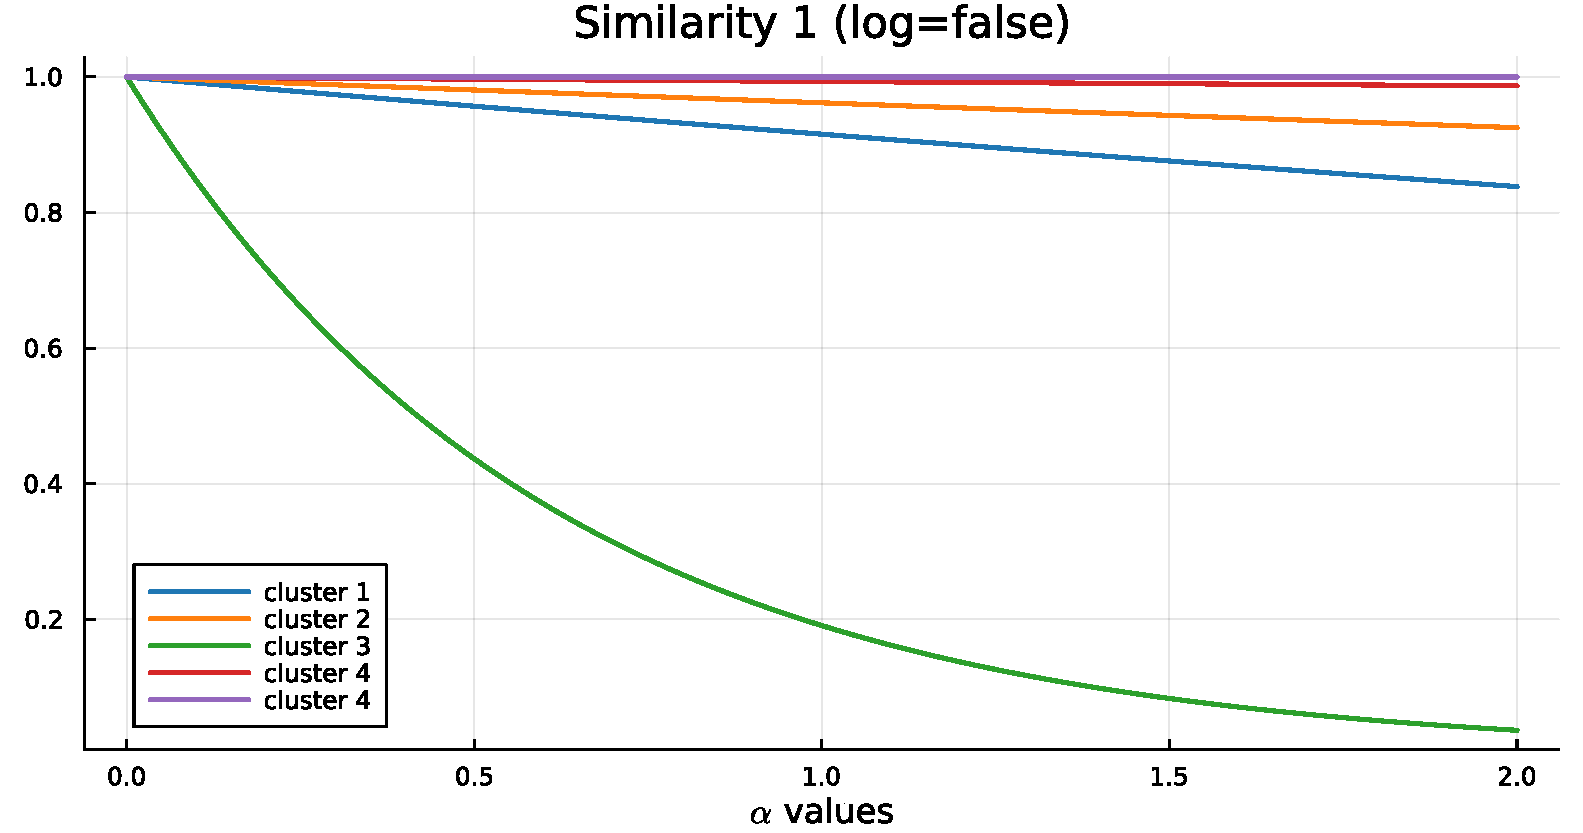
\includegraphics[width=1\linewidth]{model description/covariate similarity analysis//test case on 5 clusters/similarity1_log_false.pdf}
    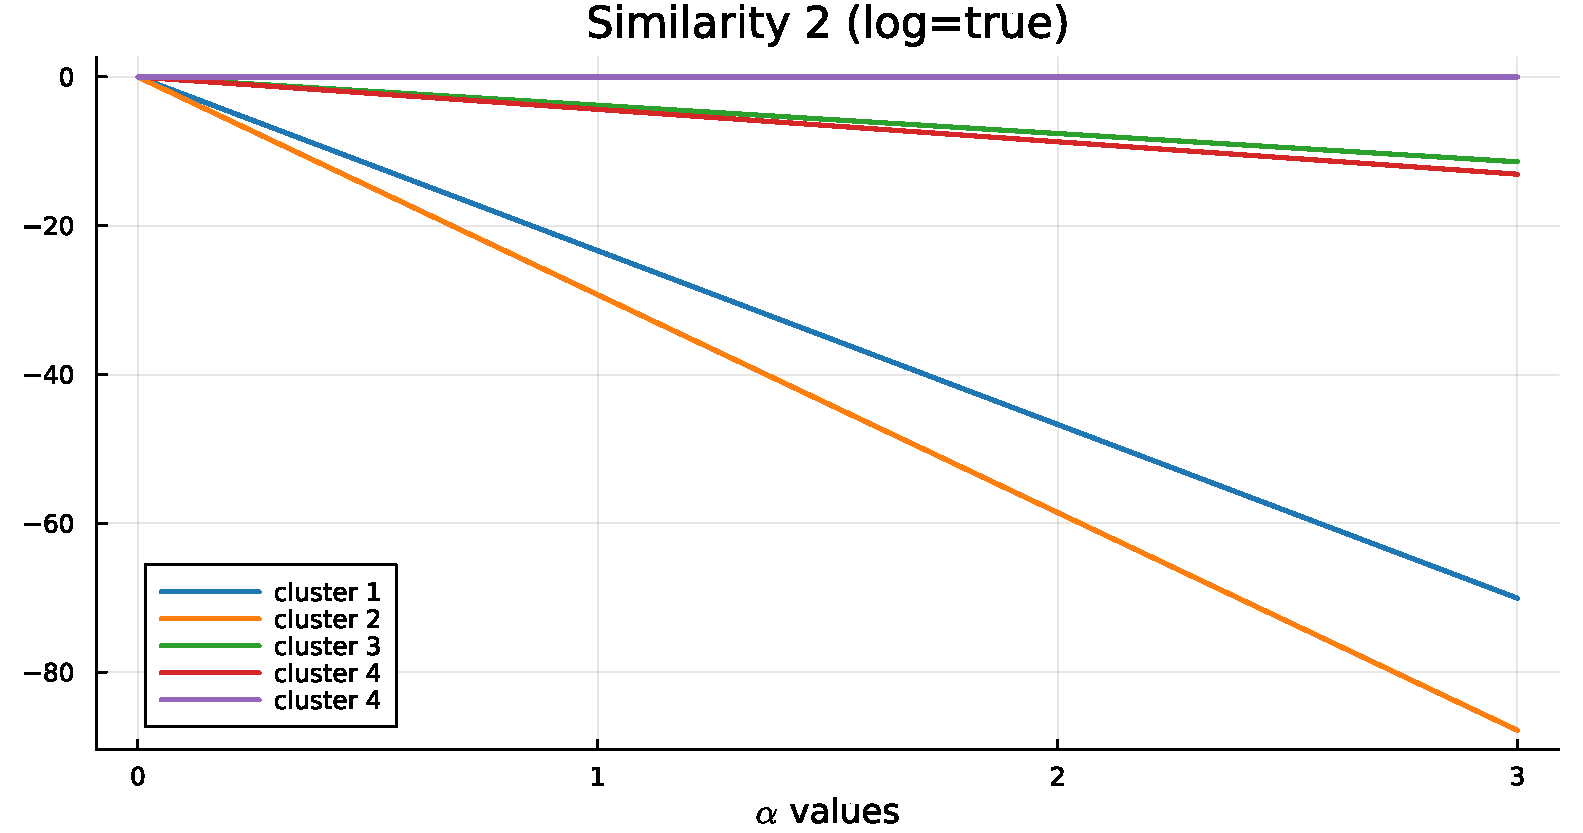
\includegraphics[width=1\linewidth]{model description/covariate similarity analysis//test case on 5 clusters/similarity2.pdf}
    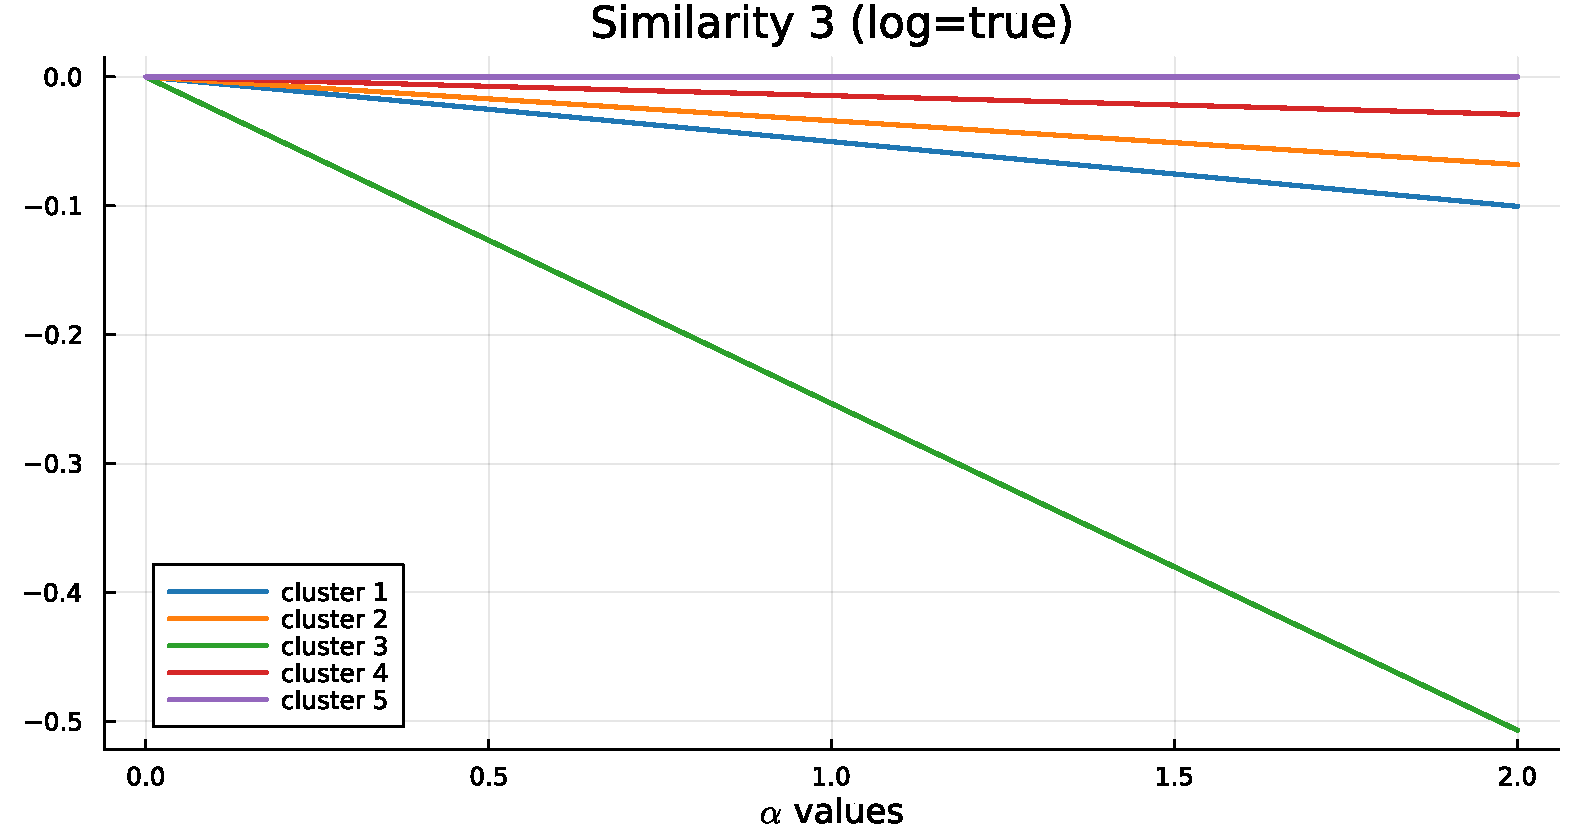
\includegraphics[width=1\linewidth]{model description/covariate similarity analysis//test case on 5 clusters/similarity3.pdf}
    \caption[Similarities 1, 2 and 3 illustration]{Similarities 1, 2 and 3 computed on the test case partition, with respect to different values of their tuning parameter. Similarity 1 is without the logarithm applied just for plotting purposes, to see more clearly the gap among the clusters.}
    \label{fig: sim123}
\end{figure}

\begin{figure}[!p]
    \centering
    % 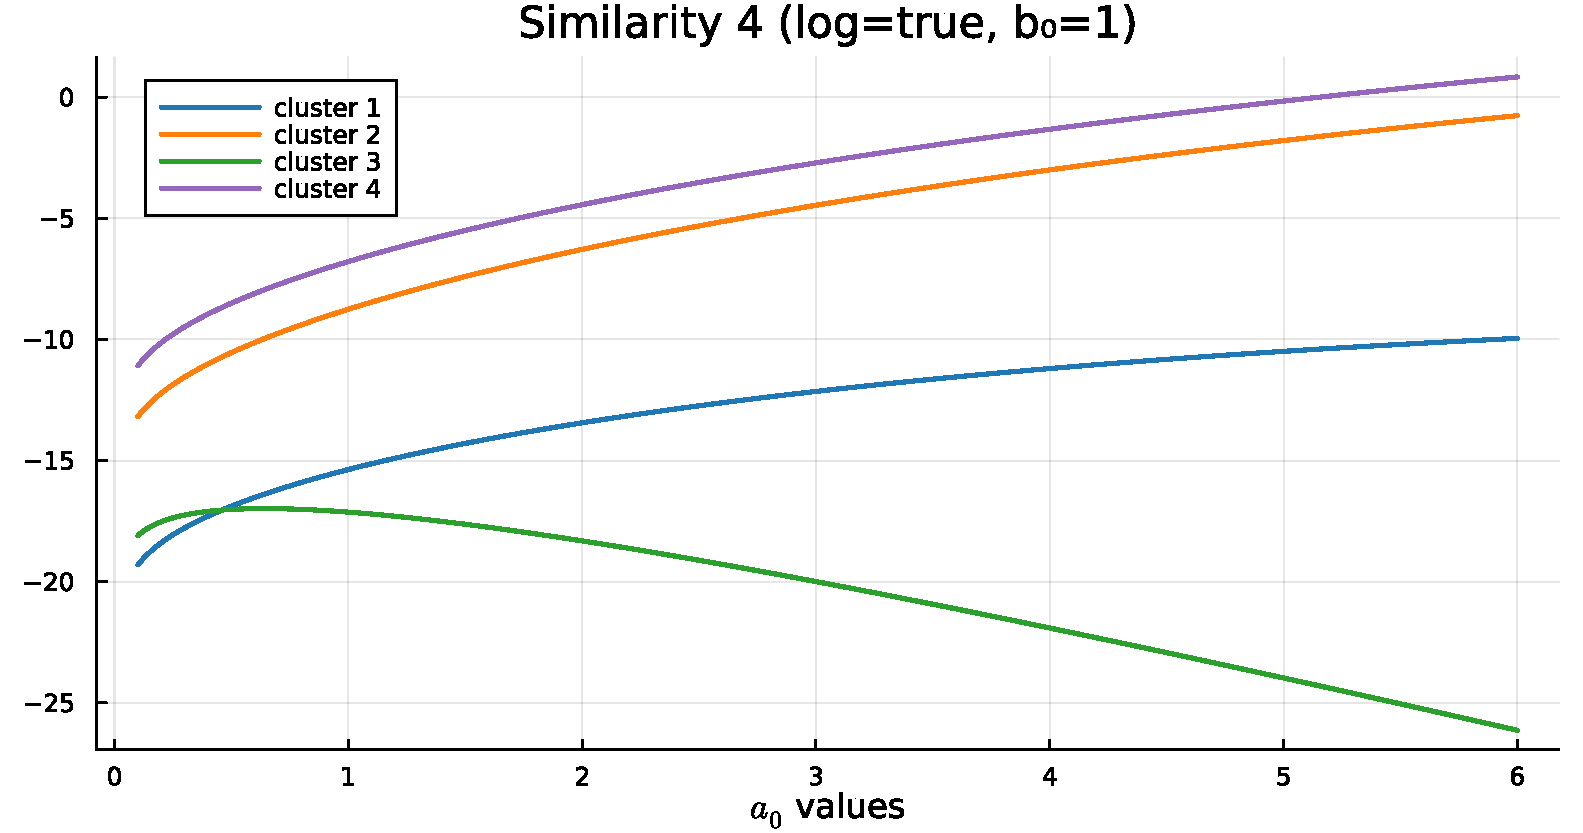
\includegraphics[width=1\linewidth]{model description/covariate similarity analysis/similarity4_lambda1_bc1.pdf}
    % 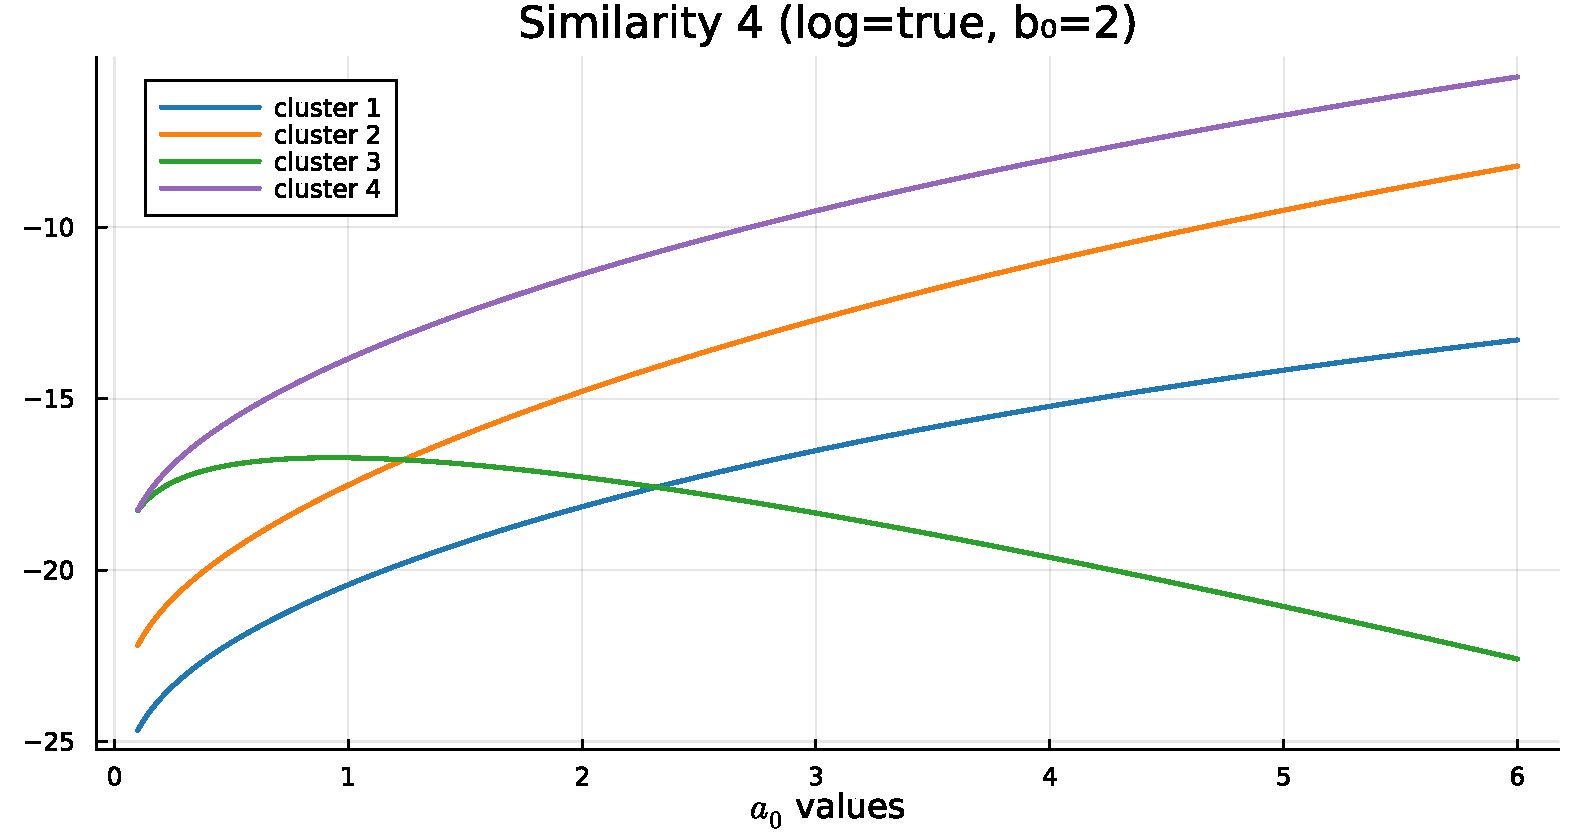
\includegraphics[width=1\linewidth]{model description/covariate similarity analysis/similarity4_lambda1_bc2.pdf}
    % 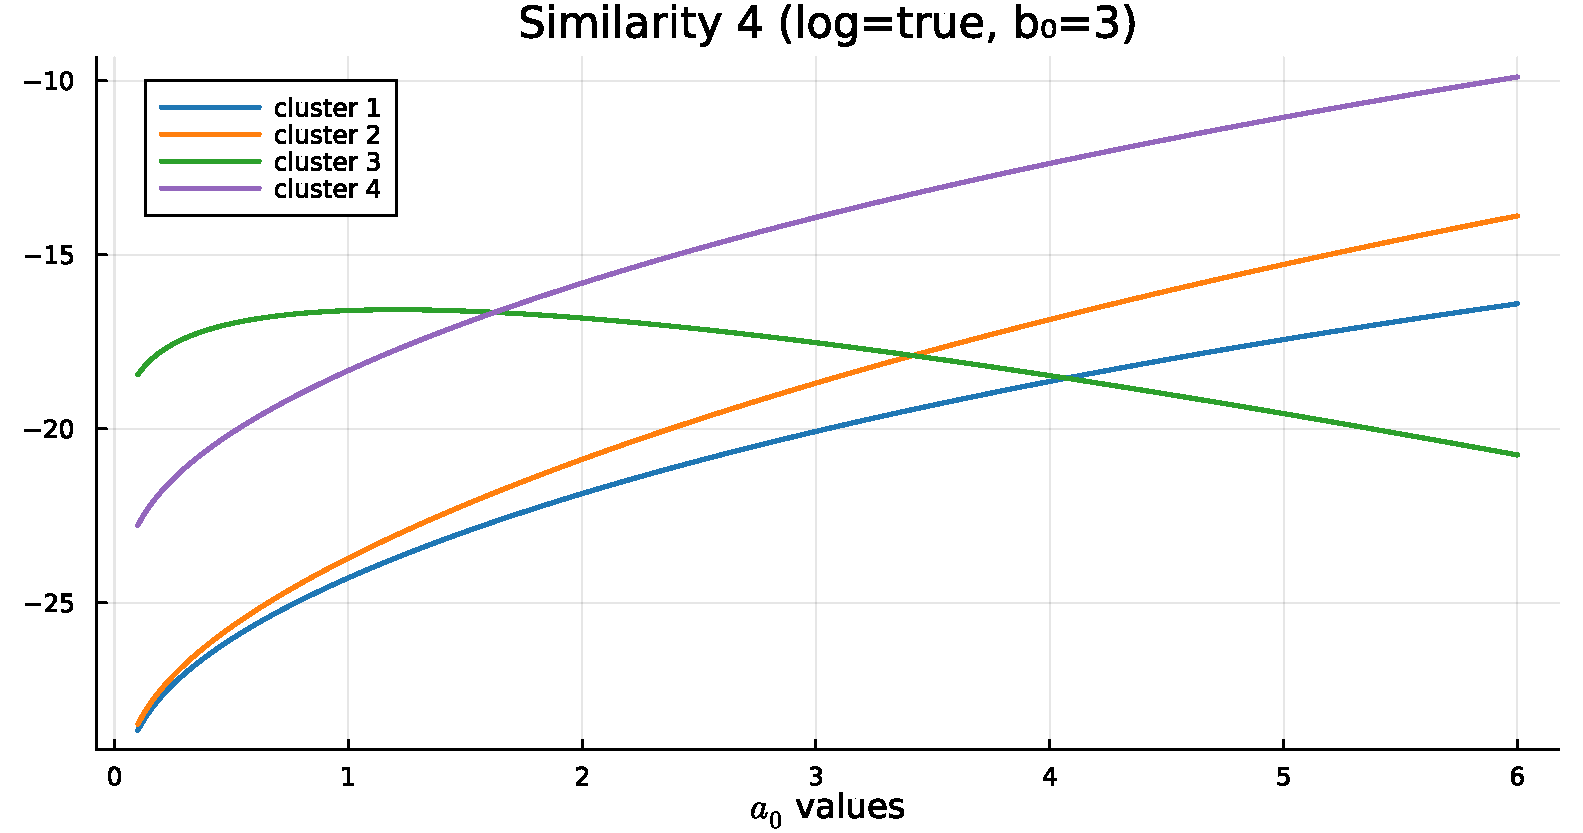
\includegraphics[width=1\linewidth]{model description/covariate similarity analysis/similarity4_lambda1_bc3.pdf}   
    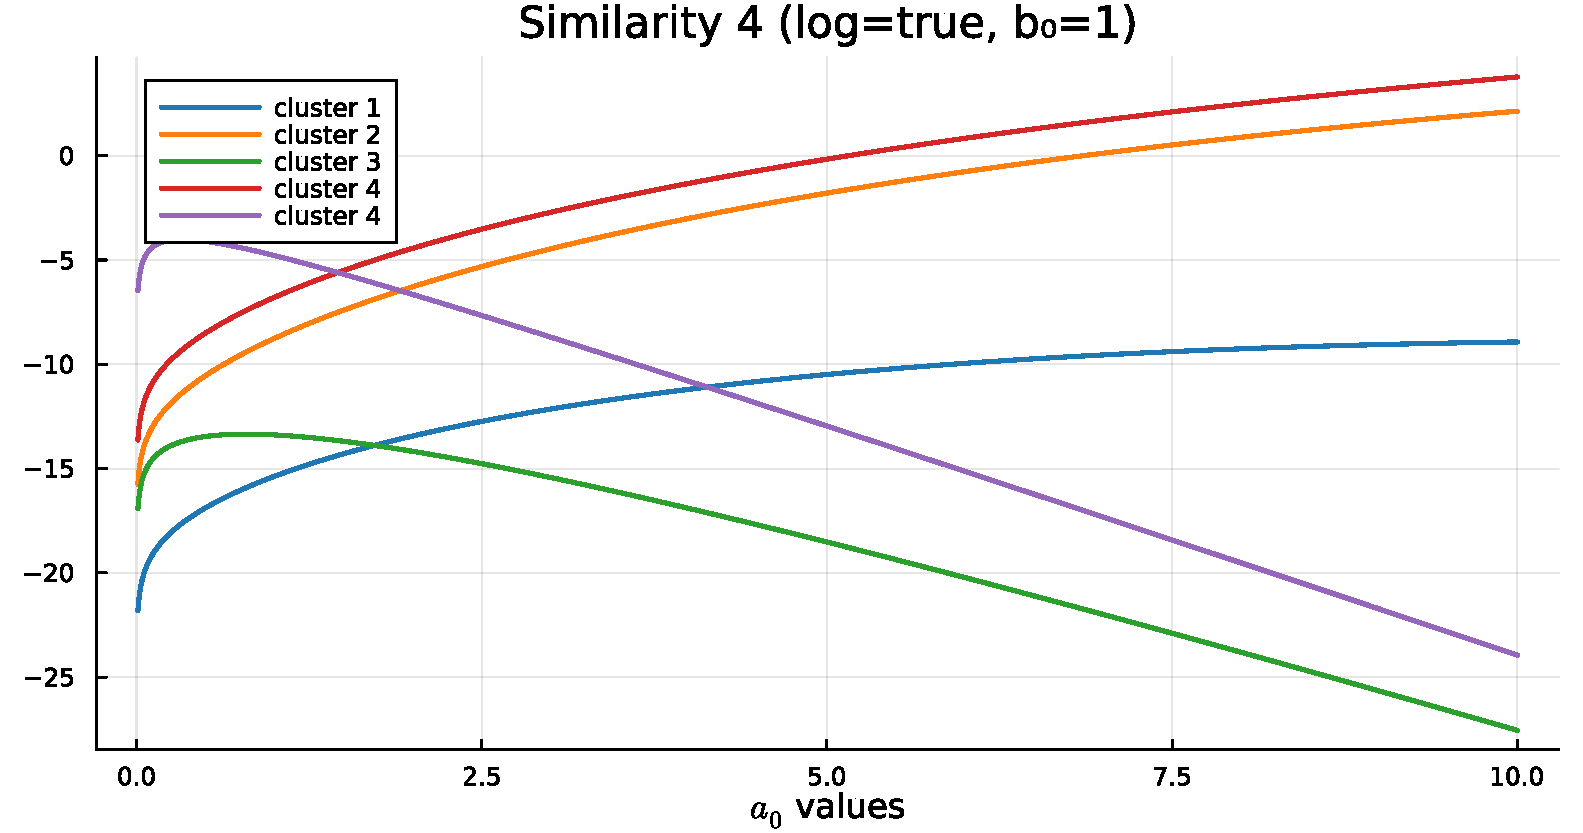
\includegraphics[width=1\linewidth]{model description/covariate similarity analysis//test case on 5 clusters/similarity4_lambda1_bc1.pdf}
    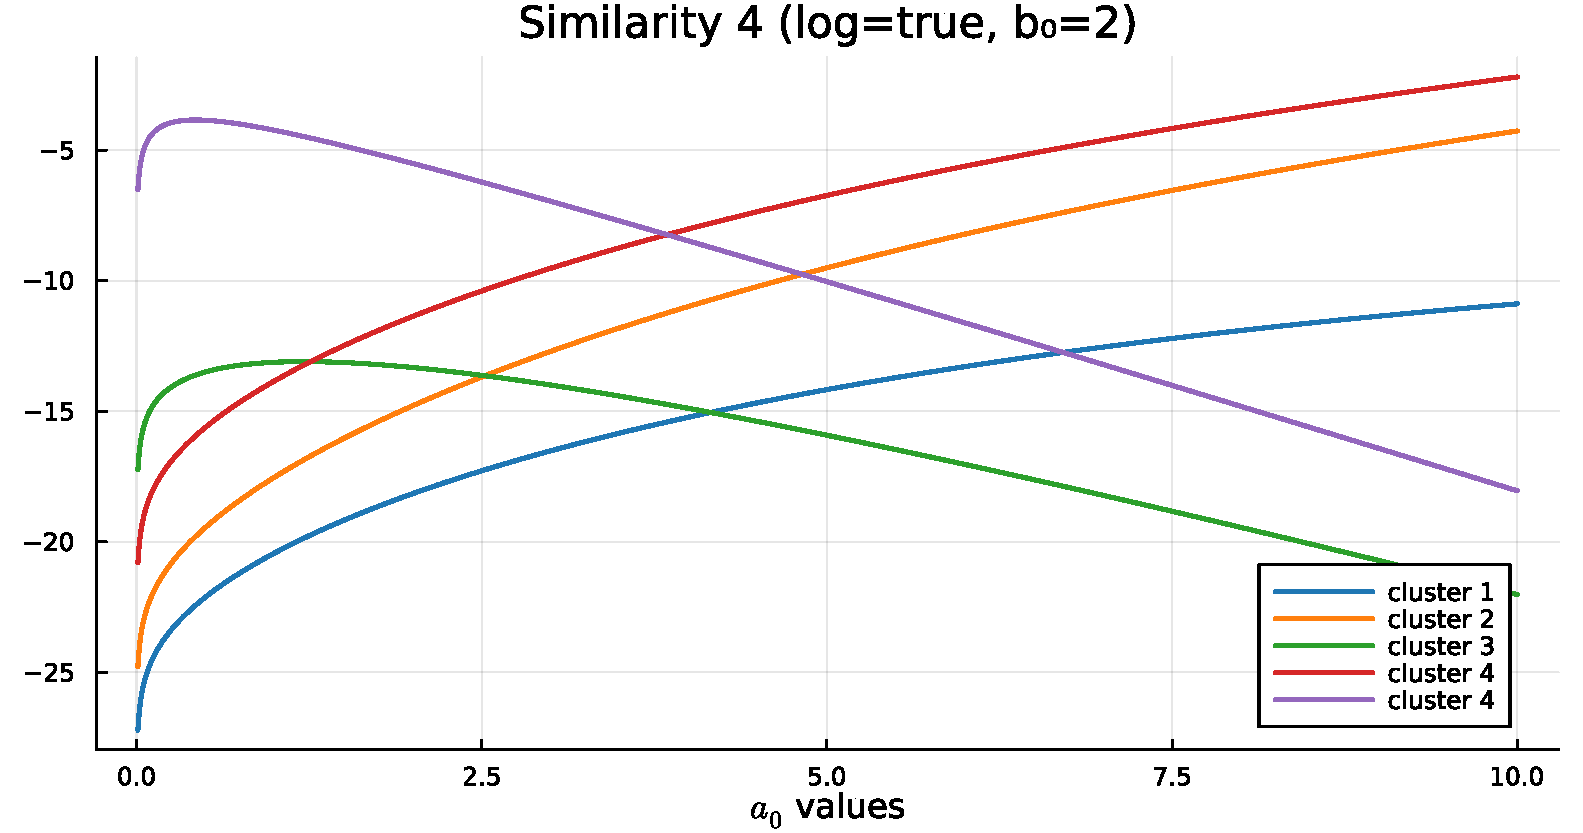
\includegraphics[width=1\linewidth]{model description/covariate similarity analysis//test case on 5 clusters/similarity4_lambda1_bc2.pdf}
    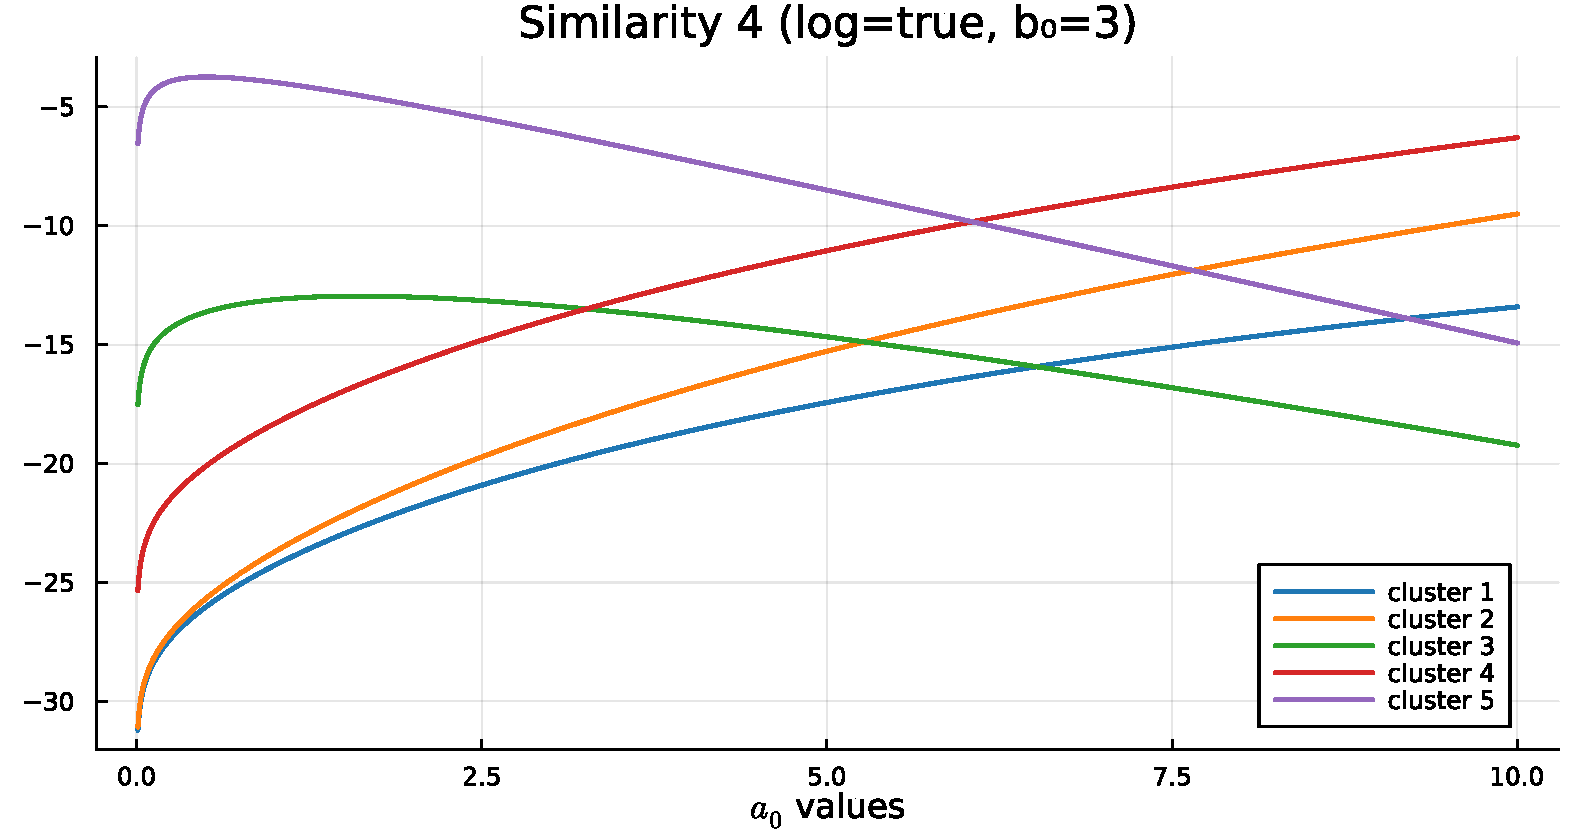
\includegraphics[width=1\linewidth]{model description/covariate similarity analysis//test case on 5 clusters/similarity4_lambda1_bc3.pdf}
    \caption[Similarity 4 illustration]{Similarity 4 computed on the test case partition, with respect to the different values of the tuning parameter $a_0$ and $b_0$. The other parameters has been set to $\mu_0=0$ and $\lambda_0=1$, with the idea to apply the similarity on scaled (centered and standardized) covariates.}
    \label{fig: sim4}
\end{figure}

Another popular choice is the Gower similarity function \cite{gower}, which was originally designed for a multivariate context, where vectors of covariates are compared to each other. As a consequence, some work was required to adapt it to the univariate case. The simple idea of comparing all cluster-specific pair-wise similarities leads to the total Gower similarity.
% \begin{equation}    
% g(S_h,\vec{x}_{h}^\star) = \expp{-\alpha \sum_{\substack{i,j \in S_h\\ i\neq j}} d(x_i,x_h) }
% \end{equation}
\begin{equation}    
g_2(S_h,\vec{x}_{h}^\star) = \expp{-\alpha \sum_{i,j \in S_h, \,i\neq j} d(x_i,x_j) }
\end{equation}
This function, however, is strictly increasing with respect to the cluster size, meaning that it will naturally tend to propose a large number of small clusters. For that reason, a correction can be applied, accounting for the size of the cluster $S_h$, leading to the average Gower similarity.
% \begin{equation}    
% g(S_h,\vec{x}_{h}^\star) = \expp{-\dfrac{2\alpha}{|S_h|(|S_h|-1)} \sum_{\substack{i,j \in S_h\\ i\neq j}} d(x_i,x_h) }
% \end{equation}
\begin{equation}    
g_3(S_h,\vec{x}_{h}^\star) = \expp{-\dfrac{2\alpha}{|S_h|(|S_h|-1)} \sum_{i,j \in S_h, \,i\neq j} d(x_i,x_j) }
\end{equation}
In both functions, $d(x_i,x_j)$ is the Gower dissimilarity between $x_i$ and $x_j$, with $d(x_i,x_j) =  |x_i - x_j|/R$ in the case of numerical covariates, being $R=\max(\vec{x}) - \min(\vec{x})$ the range of the covariate values, considering all the units independently from their cluster, while $d(x_i,x_j) = \indicator{[x_i \neq x_j]}$ in the case of categorical covariates. This is a dissimilarity since values closer to 0 refer to similar data, while values closer to 1 to dissimilar data; therefore the minus sign inside $g_2$ and $g_3$ exponents converts the function to a similarity. For the multidimensional design there are natural extensions of the $d(\vec{x}_i,\vec{x}_j)$ function.

The last similarity recalls the structure of the spatial cohesion $C_3$, where now are the covariates to be treated as if they were random variables. However, since we chose to deal with each covariate individually, in this unidimensional setting a Normal/Normal-Inverse-Gamma model is employed, with $\vec{\csi} = (\mu,\sigma^2)$, $x|\vec{\csi} \sim \N(\mu_0,\sigma^2)$, and $\mu \sim \N(\mu_0, \sigma^2/\lambda_0)$, $\sigma^2 \sim \invgamma(a_0,b_0)$, i.e. $\vec{\csi} \sim \N\invgamma(\mu_0, \lambda_0, a_0, b_0)$. A multivariate extension is thus possible trough the same modelling style of the spatial coordinates case.

\begin{equation}    
g_4(S_h,\vec{x}_{h}^\star) = \int \prod_{i \in S_h} q(x_i|\vec{\csi}_h) q(\vec{\csi}_h) \, d\vec{\csi}_h
\end{equation}

All the similarities, except for $g_2$, agree to classify the non-singleton clusters with the red being the one with the highest similarity, followed by the orange, blue, and green, as we can see from Figures \ref{fig: sim123} and \ref{fig: sim4}. Intuitively, Figure \ref{fig: similarity tests} seems to confirm this ranking, by visually reasoning about the sparsity of each cluster. Similarities $g_4$ and $g_2$ seems to be the only ones which are able to give a considerable weight also to the green partition, which is indeed sparser but collects all the large, sort of outliers, values of the covariate at test.

Regarding their flexibility, we tested their behaviour changing the testing covariate. Similarity $g_1$ appeared to be the most adaptive one, working well (i.e. returning very reasonable orders in the clusters) in every covariate we tested. However, it tends to penalize a lot sparse clusters, as we saw in the previous test case. This could suggest to maybe implement other distance metrics rather than the $L^2$ norm in the computation of $H(S_h,\vec{x}_h^\star)$. On the other hand, similarity 4 appeared to be quite sensible to the parameters regulating the $\invgamma$ distribution for $\sigma^2$, suggesting that each covariate that we want to include in the clustering process should have her properly-tuned pair of $a_0$ and $b_0$ parameters. For this reason, the JDRPM implementation can provide this flexibility in assigning separately those parameters for each clustering covariate. 


\chapter{Implementation and optimizations}
\label{Implementation and optimizations}
% questa molto forzata
% \epigraph{\itshape \flushright
% I used to float, now I just fall down
% }{--- Billie Eilish, \textit{What Was I Made For?}}


% \chapter{Implementation and optimizations}
To implement our updated model, and to do it efficiently, we decided to opt for the Julia language \cite{Julia-cite}. 
% Julia is a high-level, high-performance dynamic programming language, developed with the core idea to solve the famous "two language problem" of scientific computing. In fact, when implementing a solution to a certain problem, there is typically a trade-off between productivity and performance. High-level interpreted languages such as R, Python, or Matlab offer an easy-to-use syntax and a friendly environment which make them attractive to a wider audience and allow for a faster development, at the cost of usually lacking in execution speed. In contrast, low-level compiled languages such as C, C++, or Fortran are able to produce more efficient code, but at the cost of an higher complexity and therefore longer development stages. To narrow this gap, two-tiered architectures have also emerged, where interface logic is written in simpler high-level languages while all the hard work is delegated to more sophisticated low-level ones. This is also the case of the current implementation of the DRPM model, which calls C code from an R library interface. However, such "compromise" can often come with significant drawbacks. Julia, instead, resolves this problem proposing a new approach which provides productivity and performance at once.

Julia is a relatively new programming language that combines the ease and expressiveness of high-level languages to the efficiency and performance of low-level ones. Such balance largely achieved trough the just-in-time (JIT) compilation, implemented using the LLVM framework, together with many nice features like dynamic multiple dispatch and heavy code specialization against multiple types. This design choice allows Julia to be used interactively, in the same fashion to the R, Matlab, or Python consoles, while also supporting the more traditional program execution style of statically compiled languages such as C, C++ and Fortran. This solution provides faster development phases, since for examples code sections can be evaluated and tested line by line, guaranteeing and at the same time efficient implementations. Performances are further enhanced by the native integration of the optimized BLAS \cite{blas} and LAPACK libraries for linear algebra operations, which are often at the core of all scientific applications. Regarding productivity, instead, Julia provides an extensive ecosystem, currently comprised by more than ten thousand packages, spanning over almost all branches of science and engineering. Moreover, most of them are already highly tested and optimized, and can therefore reduce the implementation time required to the users. As an example, in this work we employed the \mjline{Distributions} \cite{JSSv098i16} \cite{Distributions.jl-2019} and \mjline{Statistics} packages, while the original C implementation had to write all the statistical functionalities from scratch. Considering all this, the Julia choice was deemed very natural.

% \section{Algorithm implementation}
% forse questa section sta meglio nel capitolo precedente

As we will see in Chapter \ref{chap: testing}, even despite the higher complexity of the model we managed to get better performance in Julia compared to the original C implementation, at the reasonable cost of a smaller increase in the memory requirements, which nowadays should not be a big deal. Anyway, this improvement was possible trough several refinements and optimizations, which we will now discuss.

\section{Optimizations}

One of the major issues encountered during the design of the fitting function in Julia was controlling the amount of memory and allocations that some functions, structures, or algorithms would require. At the beginning of the development and testing, where the correctness of the algorithm was the only priority, we saw in fact that most of the execution time was actually spent by the garbage collector of Julia, which had the burden of track all the allocated memory and reclaim the unused one in order to make it available again for new computations. 

Together with avoiding useless allocations, or in general managing more precisely the memory, another important aspect to focus on to get better performance is ensuring type stability of the function. Luckily, Julia disposes of several tools to inspect and address both problems. 

Regarding the second point, there are several packages such as \mjline{Cthulhu} or even the simple \mjline{@code_warntype} macro which allow to ensure that a function is type-stable, i.e. that the types of all variables can be correctly predicted by the compiler and stay consistent throughout the execution. Type stability is crucial for performance as it enables the compiler to generate optimized machine code, removing the load derived from dynamic type checks. In fact, Julia is dynamically typed, which means that variables do not have to be necessarily declared with their type, in contrast to fully statically typed languages such as C, and they could change it during execution. For example, a variable initialized as an integer could later become a float, or even a string. However, for performance purposes, these dynamicisms should be avoided, and those tools help to ensure that this happens. We managed to reduce all the useless type instabilities, but some are instead still present to guarantee some flexibility to the users, e.g. to select at run time the cohesion and similarity functions to use in the fit.


\begin{figure}[!ht]
    \centering
    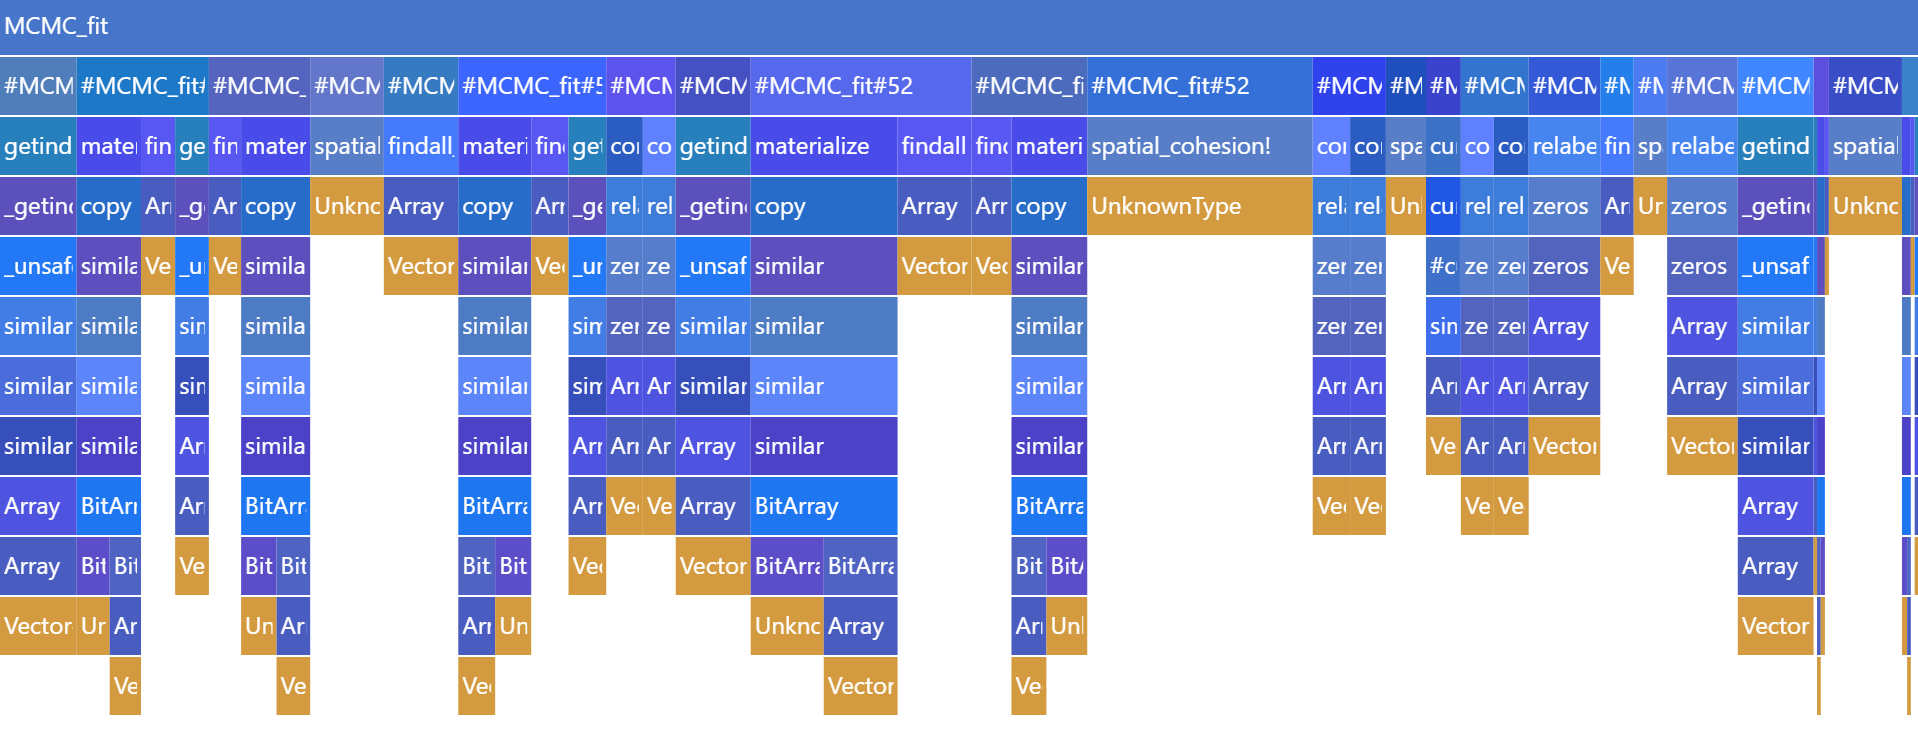
\includegraphics[width=1\linewidth]{Testing//Scaling possibilities/flame graph actual model allocs count.png}
    \caption[Flame graph of a test fit]{Flame graph derived from a simple test fit with $n=20$, $T=50$, ran for 10000 iterates. Each section, identified with a colored box, represents a function call with its stack trace below, i.e. all the other subsequent function calls generated from the initial top one. The widths are proportional to allocation counts, i.e. to how many times a memory allocation was required for their corresponding box. The plot should be read from top to bottom with respect to function calls, and from left to right with respect to the fitting steps.}
    % The syntax \texttt{\#MCMC\_fit\#k} inside the first boxes is a reference to the $k$th line in the source file.
    \label{fig: flame graph}
\end{figure}

Regarding the first point, the memory issues, we relied on the \mjline{ProfileCanvas} package. This profiler generates a plot, the flame graph, represented in Figure \ref{fig: flame graph}, which illustrates the different sections of code with regions whose size is proportional to a certain metric, e.g. the time spent on them during execution or, in this case of memory investigation, the number or size of allocations that was required for that section. This allows to see if the running time is spent on actual useful operations or instead on "bad" ones, such as garbage collection and run-time evaluations; therefore highlighting the sections of code which could possibly be optimized. All the modelling and working variables were of course preallocated, but the key idea has been to refactor the code to make it work more \textit{in place}, passing as arguments the variables which would be modified by the function and applying those changes directly inside the function, rather than returning some values and then use them to modify the initial variables.

More in general, also the \mjline{BenchmarkTools} \cite{BenchmarkTools.jl-2016} package has been a great tool to quickly analyse and compare entire fits or just small sections of code. For example, that package allows to simply test different versions of equivalent instructions to see which one could be the most efficient, as in this case
\begin{code}
\begin{minted}
[
breaklines,
baselinestretch=1,
autogobble,
% breaksymbolsepleft=2,
fontsize=\footnotesize,
% linenos
mathescape,
tabsize=4,obeytabs
]{julia}
using BenchmarkTools
nh_tmp = rand(100)
@btime nclus_temp = sum($nh_tmp .> 0)
# 168.956 ns (2 allocations: 112 bytes)
@btime nclus_temp = count(x->(x>0), $nh_tmp)
# 11.612 ns (0 allocations: 0 bytes)
\end{minted}
\end{code}
or this other one
\begin{code}
\begin{minted}
[
breaklines,
baselinestretch=1,
autogobble,
% breaksymbolsepleft=2,
fontsize=\footnotesize,
% linenos
mathescape,
tabsize=4,obeytabs
]{julia}
n = 100; rho_tmp = rand((1:5),n); k = 1
@btime findall(j -> ($rho_tmp)[j]==$k, 1:n) # with anonymous function
# 272.302 ns (5 allocations: 384 bytes)
@btime findall_faster(j -> ($rho_tmp)[j]==$k, 1:n) # custom implementation 
# 214.259 ns (3 allocations: 960 bytes)
@btime findall($rho_tmp .== $k) # with element-wise comparison
# 184.112 ns (3 allocations: 320 bytes)
\end{minted}
\end{code}
where the \mjline{$} symbol is used for interpolating a variable, ensuring to treat it as a local variable inside the benchmark and therefore avoiding any performance bias caused by accessing a global variable. This was a quick and simple comparison, yet very precise and effective, which would be instead more complex to replicate in C.

During the finer and final refinements of the code we also used more low-levels analysis tools such as the \mjline{--track-allocation} option, which asks Julia to execute the code and annotate the source file to see at which lines, and of which amount, allocations occur.

\subsection{Optimizing spatial cohesions}

The memory allocation problem was especially visible in the spatial cohesion computation. In fact, such computation appears in both sections of updating $\gamma_{it}$ and updating $\rho_t$, which are inside of outer loops on draws, time, and units, and involve themselves some other loops on clusters. All this implied that those cohesion computations will be executed possibly millions of times during each fit. A simple and quick inspection suggests a value between $dTn$ and $dTn^2$, being $d$ the number of iterations, $T$ the time horizon and $n$ the number of units. We can't provide more precise estimate due to the variability and randomicity of the inside loops, which depend on the distribution of the clusters. With all that in mind, it was crucial to optimize the performance of the cohesion functions.

The only optimizing task consisted in carefully designing the cohesion function implementations. Cohesions 1, 2, 5 and 6 didn't exhibit any complication or need for optimization: the natural conversion in code from their mathematical models proved to be already optimally performing. The main problem was instead with cohesions 3 and 4, the auxiliary and double dippery, which by nature would involve some linear algebra computations with vectors and matrices. 

The first implementation of those cohesions turned out to be really slow, due to the overhead generated by allocating and then freeing, at each call, the memory devoted to all vectors and matrices. This in the end meant that most of the execution time was actually spent by the garbage collector, rather than in the real and useful operations. A first solution was then to resort to a scalar implementation, which would remove the overhead of the more complex memory structures. In the end, we managed to combine the readability of the first idea with the performance of the second one into a final version, as we can see from Listing \ref{list: cohes3}.

\begin{code}
\caption[Different cohesion 4 implementations]{Sections of the Julia code for the three implementation cases of the spatial cohesions 3 and 4. The first one has the first-thought vector implementation derived from the mathematical formulation, the second one is the conversion to only have scalar variables, while the third one is the final version, keeping the vector form but improved using static structures.}
\label{list: cohes3}
\begin{minted}
[
breaklines,
baselinestretch=1,
autogobble,
% breaksymbolsepleft=2,
fontsize=\footnotesize,
% linenos
mathescape,
tabsize=4,obeytabs
]{julia}
# original vector version
sbar = [mean(s1), mean(s2)]
vtmp = sbar - mu_0
Mtmp = vtmp * vtmp'
Psi_n = Psi + S + (k0*sdim) / (k0+sdim) * Mtmp

# scalar-only version
sbar1 = mean(s1); sbar2 = mean(s2)
vtmp_1 = sbar1 - mu_0[1]
vtmp_2 = sbar2 - mu_0[2]
Mtmp_1 = vtmp_1^2
Mtmp_2 = vtmp_1 * vtmp_2
Mtmp_3 = copy(Mtmp_2)
Mtmp_4 = vtmp_2^2
aux1 = k0 * sdim; aux2 = k0 + sdim
Psi_n_1 = Psi[1] + S1 + aux1 / (aux2) * Mtmp_1
Psi_n_2 = Psi[2] + S2 + aux1 / (aux2) * Mtmp_2
Psi_n_3 = Psi[3] + S3 + aux1 / (aux2) * Mtmp_3
Psi_n_4 = Psi[4] + S4 + aux1 / (aux2) * Mtmp_4

# static improved version
sbar1 = mean(s1); sbar2 = mean(s2)
sbar = SVector((sbar1, sbar2))
vtmp = sbar .- mu_0
Mtmp = vtmp * vtmp'
aux1 = k0 * sdim; aux2 = k0 + sdim
Psi_n = Psi .+ S .+ aux1 / (aux2) .* Mtmp
\end{minted}
\end{code}

This final version exploits the \mjline{StaticArrays} package of Julia, which allows to use vectors and matrices more efficiently if their size is known at compile time; which is the case of the spatial cohesions computation since working with planar spatial coordinates we will always have $2\times 1$ vectors and $2 \times 2$ matrices. The benefits of this final version are that we maintain the natural mathematical form of the first one, improving the clearness of the code, together with the efficiency of the second one, since now with static structures the compiler is able to optimize all memory allocations as it was doing with the simple scalar variables.


\begin{figure}[h!]
\centering
\begin{tabular}{cc}
    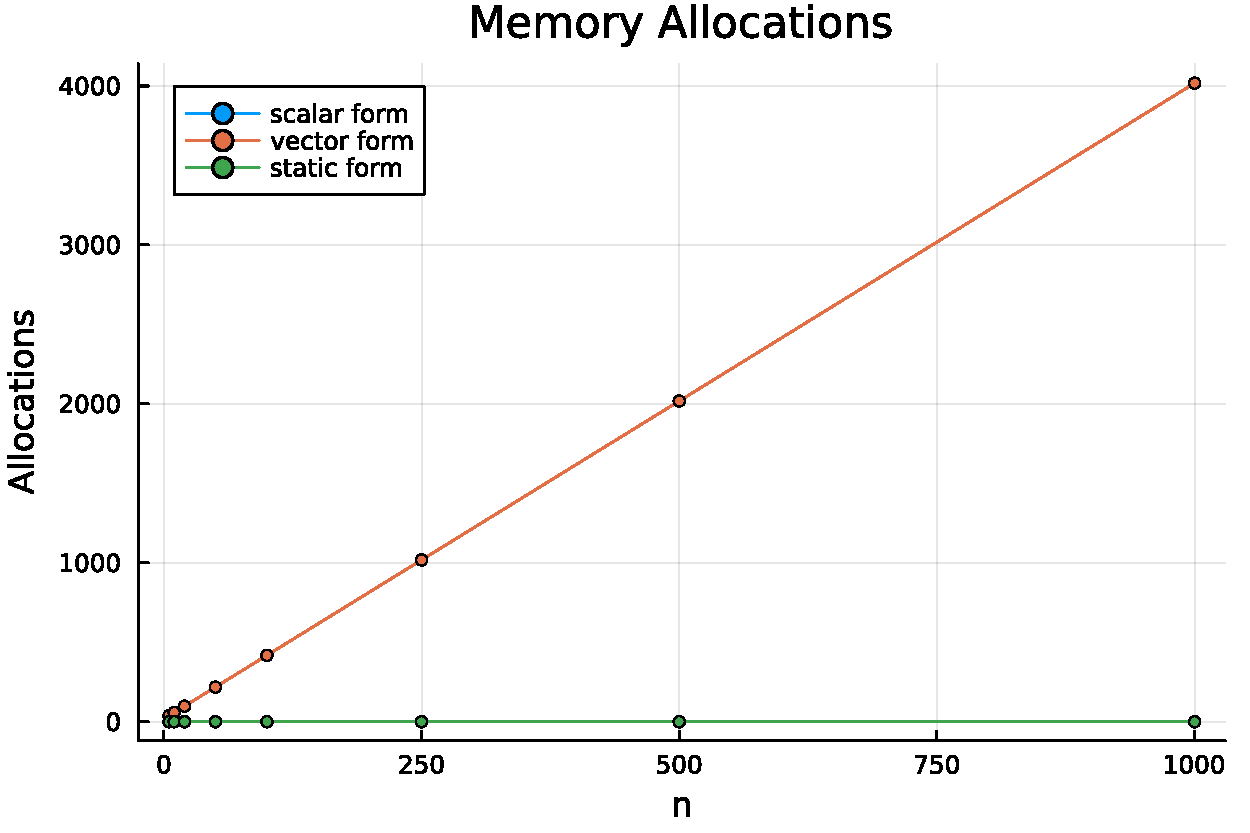
\includegraphics[width=0.5\linewidth]{Plots/memory_allocations.pdf} &    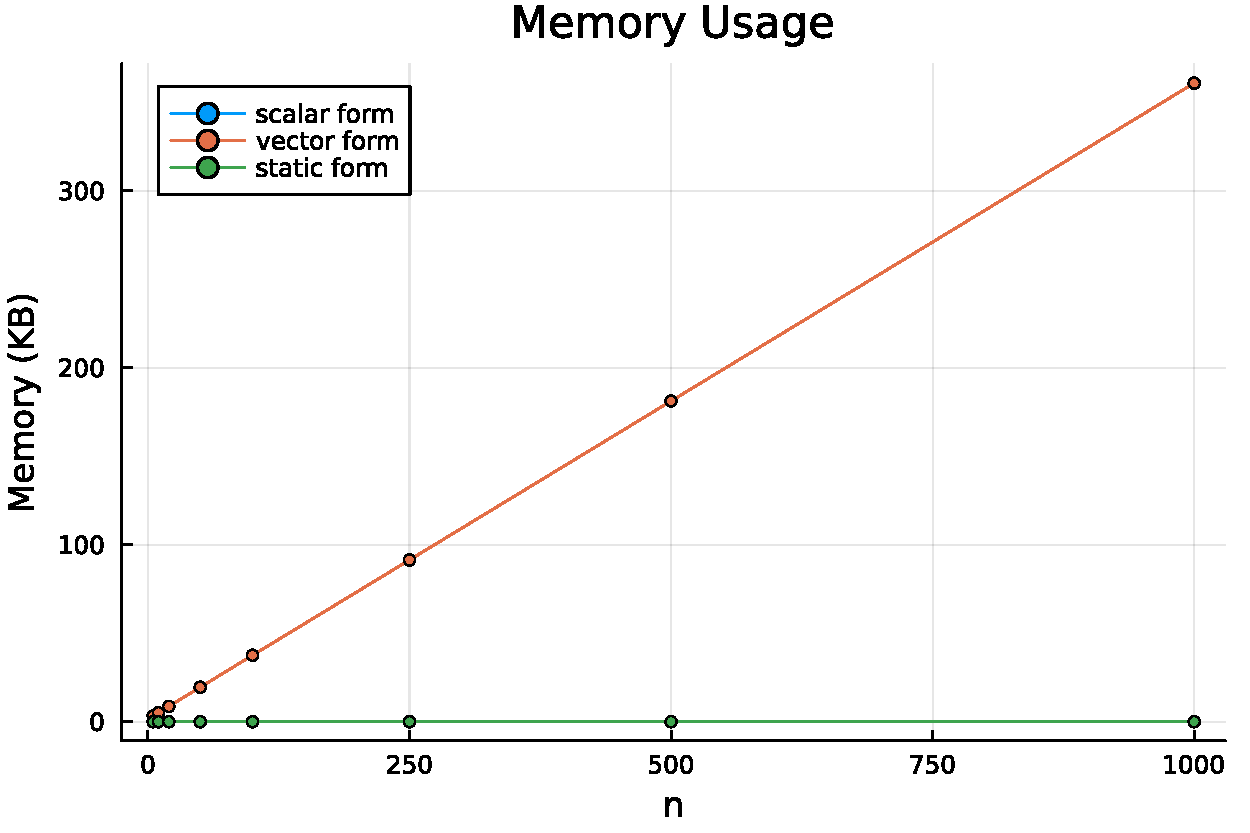
\includegraphics[width=0.5\linewidth]{Plots/memory_usage.pdf} \\  
    \multicolumn{2}{c}{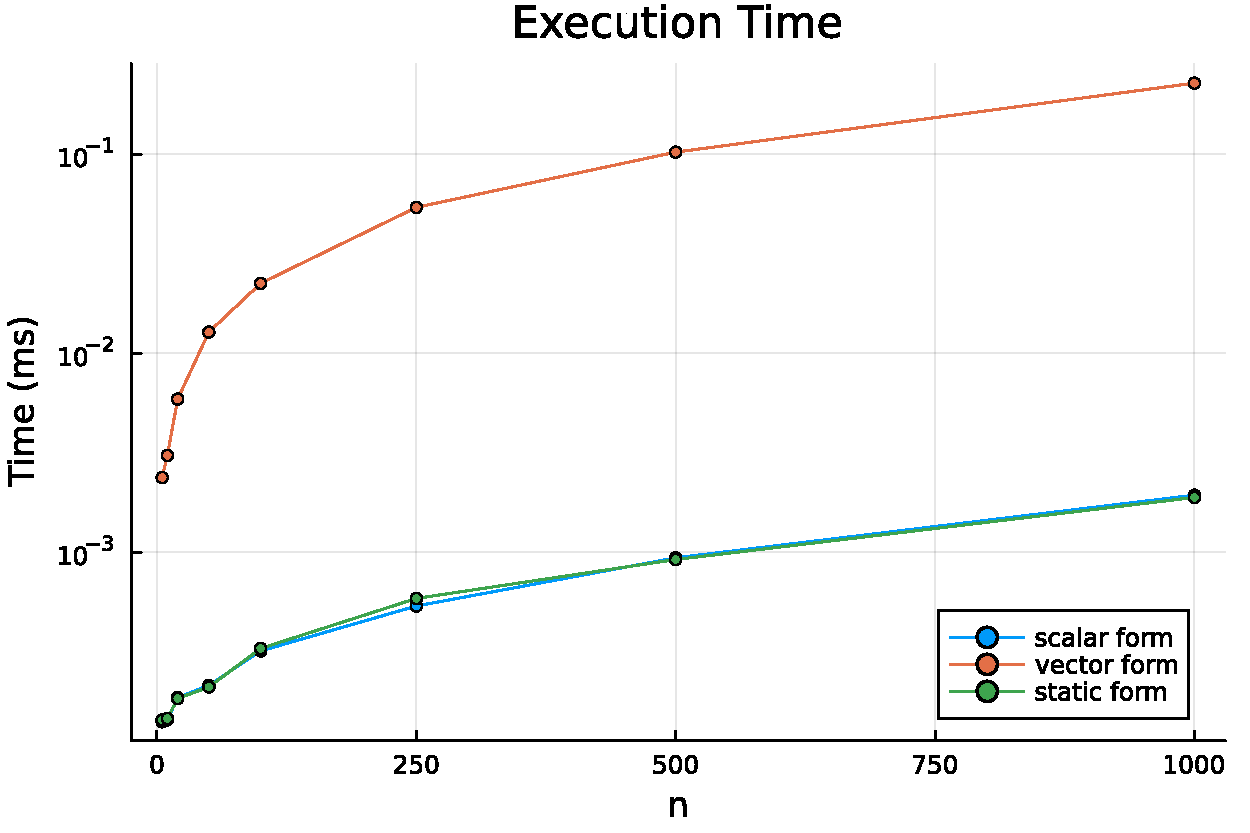
\includegraphics[width=1\linewidth]{Plots/execution_time.pdf} }\\
\end{tabular}
\caption[Cohesions 3 and 4 implementation comparison]{Performance comparison between the three versions of the cohesion 4 function. Tests ran through the \mintinline{julia}{BenchmarkTools} package of Julia by randomly generating the spatial coordinates of the various test sizes $n$, with similar results standing for cohesion 3. The memory allocation and usage plots are constant at zero for both the scalar and vector static cases.}
\label{fig: cohesion3 comparison}
\end{figure}


Figure \ref{fig: cohesion3 comparison} shows the comparison of their performances, where we can see how the scalar and static versions indeed perform very similarly to each other, and more quickly with respect to the first version.

Noticeably, the C implementation of the model didn't have to worry about all this reasoning, since C can't natively, nor gracefully, work with vectors and matrices and was therefore forced to the scalar implementation. 
% So one point for the old lad.


% \section{Covariates similarities optimized computation}
\subsection{Optimizing covariates similarities}
Another problem has been understanding how to speed up the computation of the similarity functions, since those would also be called possibly millions of times as the cohesion ones or even more, considering that we can incorporate more than one covariate into the clustering process, and this would add an additional loop based on $p$, the number of covariates decided to be included.

As in the previous case, some of the functions didn't show any special need or room for relevant optimizations. The fourth one instead, the auxiliary similarity function, was essential to be optimized: not only because it is one the most common choice among the similarities, but also because it involves a computationally heavy sum of the squares of the covariate values, as we can see in Listing \ref{list: sim4}.

\begin{code}
\caption[Similarity 4 implementation]{Version of the similarity 4 function with all the possible optimizing macros. The performance analysis will focus just on that inside loop, since the rest is not negotiable.}
\label{list: sim4}
\begin{minted}
[breaklines,
baselinestretch=1,
autogobble,
% breaksymbolsepleft=2,
fontsize=\footnotesize,
% linenos
mathescape,
tabsize=4,obeytabs
]{julia}
function similarity4(X_jt::AbstractVector{<:Real}, mu_c::Real, lambda_c::Real, a_c::Real, b_c::Real, lg::Bool)
	n = length(X_jt)
	nm = n/2
	xbar = mean(X_jt)
	aux2 = 0.
	@inbounds @fastmath @simd for i in eachindex(X_jt)
		aux2 += X_jt[i]^2
	end
	aux1 = b_c + 0.5 * (aux2 - (n*xbar + lambda_c*mu_c)^2/(n+lambda_c) + lambda_c*mu_c^2 )
	out = -nm*log2pi + 0.5*log(lambda_c/(lambda_c+n)) + lgamma(a_c+nm) - lgamma(a_c) + a_c*log(b_c) + (-a_c-nm)*log(aux1)
	return lg ? out : exp(out)
end
\end{minted}
\end{code}

The idea to optimize it has been to annotate the loop with some macros provided by Julia. They are the following:
\begin{itemize}
    \item \mjline{@inbounds} eliminates the array bounds checking within expressions. This allows to skip those checks to save some execution time. This insertion is harmless as long as we are sure that in our code design no out-of-bounds or wrong accesses will occur. Otherwise some undefined behaviour will take place. The above loop is indeed very simple and safe, so this assumption is clearly satisfied. 
    
    \item \mjline{@fastmath} executes a transformed version of the expression which calls functions that may violate strict IEEE semantics\footnote{Institute of Electrical and Electronics Engineers. The IEEE-754 standard defines floating-point formats, i.e. the ways to represent real numbers in hardware, and the expected behaviour of arithmetic operations on them, including precision, rounding, and handling of special values (e.g. NaN (Not a Number) and infinity).}. For example, its use could make $(a+b)+c \neq a+(b+c)$, but just in very pathological cases. Again, this is not a problem in our function, where we are just computing $\sum X_i^2$, since it does not have an intrinsically "right order" in which it has to be done.
    
    \item \mjline{@simd} (single instruction multiple data) annotate a for loop to allow the compiler to take extra liberties to allow loop re-ordering. This is a sort of parallelism technique, but rather than distributing the computational load on more processors we just \textit{vectorize} the loop, i.e. we enable the CPU to perform that single instruction (summing the square of the $i$-th component to a reduction variable) on multiple data chunks at once, using vector registers, rather than working on each element of the vector individually.
\end{itemize}

As we can see from Figure \ref{fig: exec time sim}, the actual performance difference basically derives just from the use of \mjline{@simd}, with the other two annotations making not much of a difference. For that reason, and to reassure all pure mathematicians, we decided to remove the \mjline{@fastmath} annotation, leaving just \mjline{@inbounds} and \mjline{@simd}.


\begin{figure}[h]
    \centering
    % 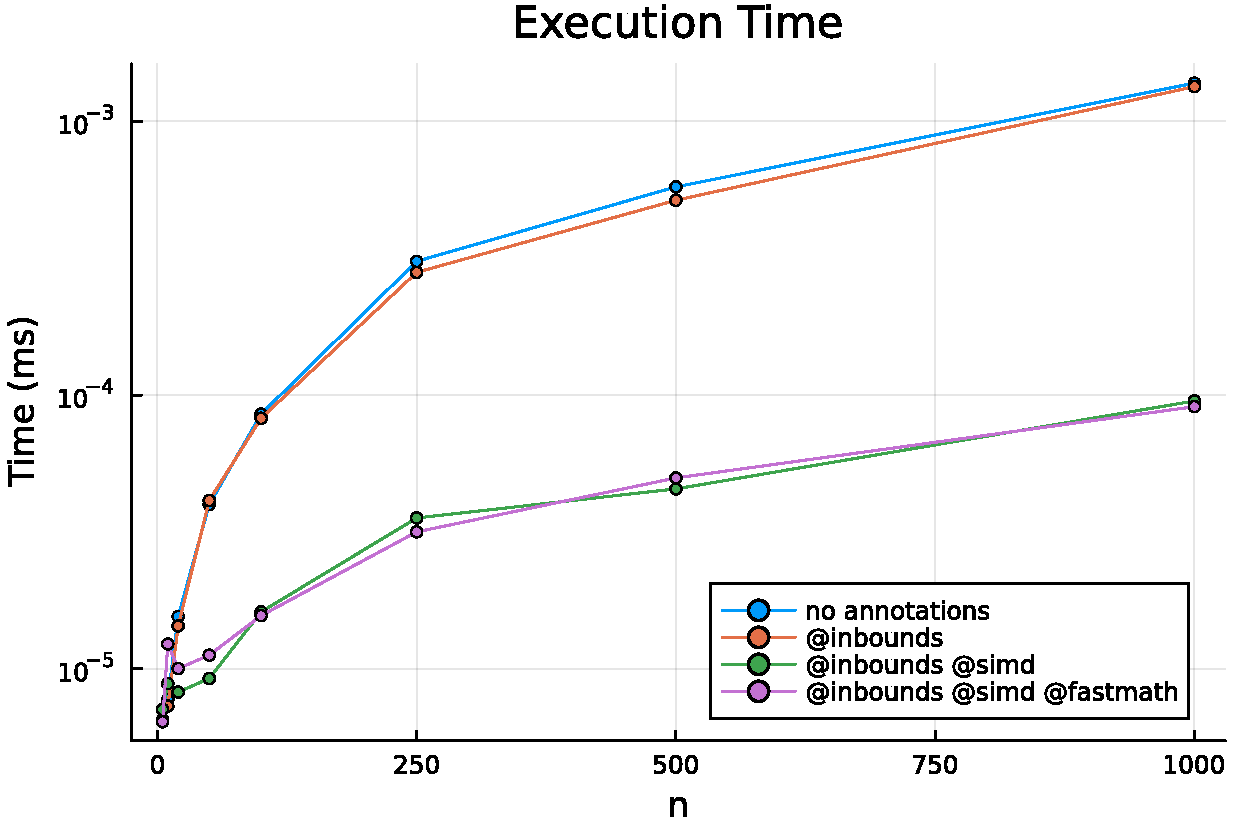
\includegraphics[width=1\linewidth]{Plots/execution_time_tests_sims.pdf}
    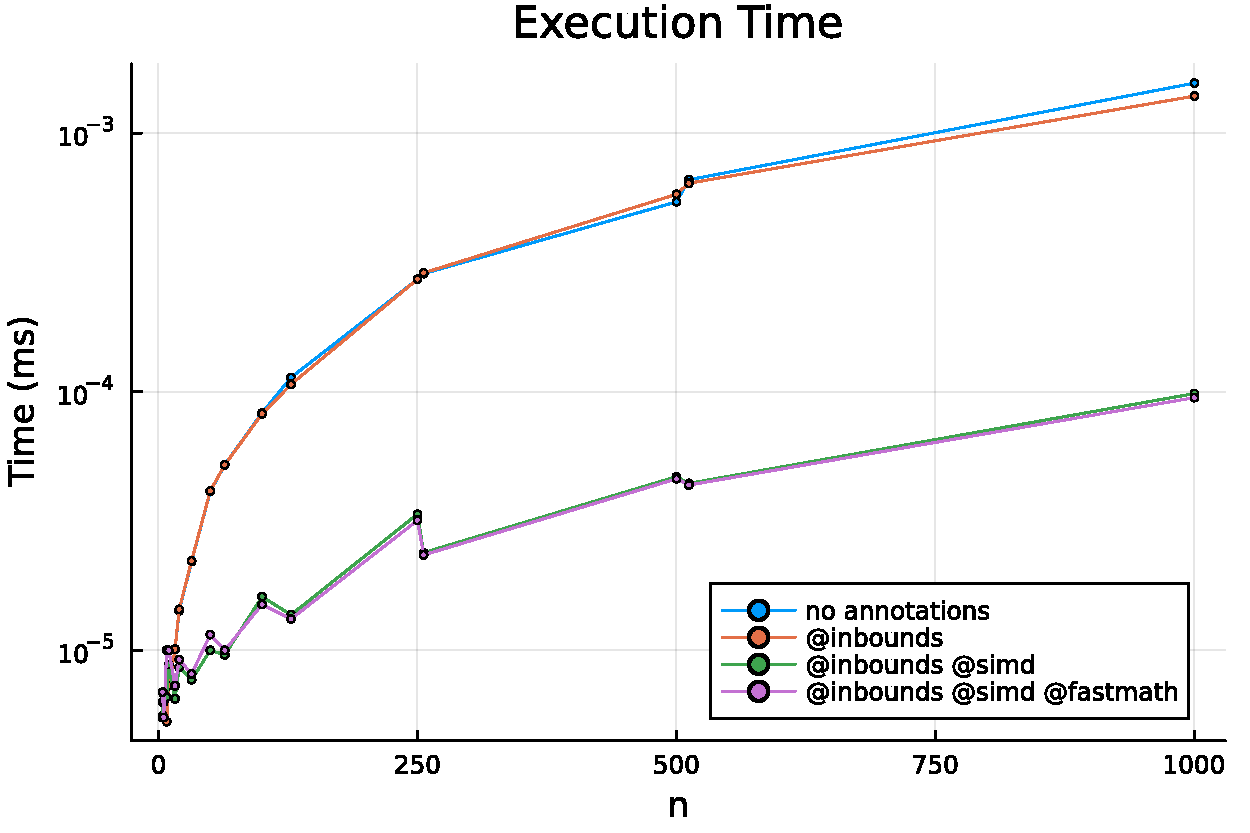
\includegraphics[width=1\linewidth]{Plots/execution_time_tests_sims_pow2.pdf}
    \caption[Similarity 4 annotations comparison]{Comparison of the performances of the different possible loop annotations in the similarity 4 implementation. Their numerical output results are indeed the same for all cases. There are no memory allocation and usage plots since the analysis has been conducted only to evaluate the performances of the inside loop, which has no memory issues.}
    \label{fig: exec time sim}
\end{figure}

We can also notice interestingly how the tests with \mjline{@simd} annotation run quicker in the case of $n$ being a power of two, compared to their closest rounded integers (e.g. 256 against 250 or 512 against 500), despite having relatively some more data. This is a proof of the effectiveness of the SIMD paradigm: according to the different architectures, the CPUs can provide different register sizes (e.g. 64, 128, 256 or 512 bits) and therefore the data subdivision can fit perfectly in them when the total memory occupied by the elements is a multiple of that register size (i.e. the number of data values is a power of two). Otherwise there will be some "leftovers chunks", which will of course be processed, but will also cause, as a consequence of the imperfect fit, a bit of overhead.





\chapter{Testing}
\label{chap: testing}

% \setlength\epigraphwidth{.65\textwidth}
% \epigraph{\itshape
% I admit that twice two makes four is an excellent thing, but if we are to give everything its due, twice two makes five is sometimes a very charming thing too.
% }{--- F\"{e}dor Dostoevskij, \textit{Notes from the Underground}}
% \setlength\epigraphwidth{.8\textwidth}

\section{Assessing the equivalence of the models}
% \section{Base comparison of the models}
Our model, and the corresponding Julia code, is just an improvement of the original DRPM with his relative C implementation. These improvements, as described in the previous chapters, refer to the insertion of covariates, both at the clustering and likelihood levels, the handling of missing values in the target variable, and the computational efficiency. In this sense, our updates are just add-ons to the original model, and therefore at a common testing level they should perform similarly by agreeing in the clusters that they produce on a given dataset.

To assess this ideally equivalent behaviour we ran two tests: the first one with only the target values, using synthetic data, while the second including spatial information, using a real spatio-temporal dataset. For the sake of clarity, also in these sections we will refer to CDRPM for the original model and implementation from \cite{1-drpm}, while to JDRPM for the updated version derived from this thesis work.

In the following analysis we will heavily rely on the Adjusted Random Index (ARI) \cite{ari-paper} to compare the partitions generated by the models. The ARI index is a correlation index to measure similarities between clusterings. More precisely, given two partitions $\rho_1$ and $\rho_2$, the $\ari(\rho_1,\rho_2)$ returns a value between $[-1,1]$ where higher values indicates higher levels of agreement between the partitions, i.e. they produced similar clusters. Being a \textit{random} index, it has an expected value and it is equal to zero, which corresponds to the case of comparing two randomly generated partitions. 

We will use this index both to study the time evolution of the clusterings, to see e.g. if $\rho_{t+k}$ is correlated to $\rho_{t}$, that is, if the clusters show the time dependent structure that the models implement, and also to check the level of agreement between the two models, comparing the clusters produced by CDRPM and JDRPM.

All the following tests have been performed on my laptop, which for performance references  has 8 GB of RAM and 1.80 GHz CPU base clock speed, and trough the software R \cite{R-cite}, thanks the \tt{JuliaConnectoR} library \cite{juliaconnectoR} which allowed the interface between R and Julia, where JDRPM is implemented. The DPRM model corresponding to the original formulation was already available in R trough the \tt{drpm} library.

\subsection{Target variable only}
\label{Target variable only}

For the first test we generated a dataset of $n=10$ units and $T=12$ time instants, and fitted both models collecting 1000 iterates derived from 10000 total iterations, discarding the first 5000 as burnin and thinning by 5. Those parameters, as well as the generating function, were the same of \cite{1-drpm}. The generating function allowed to create data points with temporal dependence, which could be tuned trough some dedicated parameters. Both models were fitted using the full formulation, i.e. including and updating also the optional autoregression parameters $\eta_{1i}$, and $\phi_1$, and using a time specific $\alpha$.


\begin{table}[!htb]
    \caption[Accuracy metrics of CDRPM and JDRPM fits, target values only]{Summary of the comparison between the two fits on target values only. The MSE columns refer to the accuracy between the fitted values generated by the models (estimated by taking the mean and the median of the returned 1000 iterates) and the true values of the target variable. Higher LPML and lower WAIC indicate a better fit.}
    \centering
    \begin{tabular}{cccccc}
    \toprule
          % & \multicolumn{2}{c}{MSE using} & \multicolumn{2}{c}{Fit metrics} & \\
           % \cmidrule(lr){2-3}
           % \cmidrule(lr){4-5}
           & MSE mean &  MSE median & LPML & WAIC & exec. time  \\
           % & mean &  median & LPML & WAIC & execution time  \\
           \midrule
        CDRPM &  1.6731  & 1.5861  & -249.61 & 469.69 & 4.8s\\
        JDRPM & \textbf{1.2628}  & \textbf{1.2181}  & \textbf{-227.83} &  \textbf{415.03}  &  \textbf{2.5s} \\
        \bottomrule
    \end{tabular}
    \label{tab: fits metrics no space}
\end{table}

\begin{figure}[!htb]
    \centering
    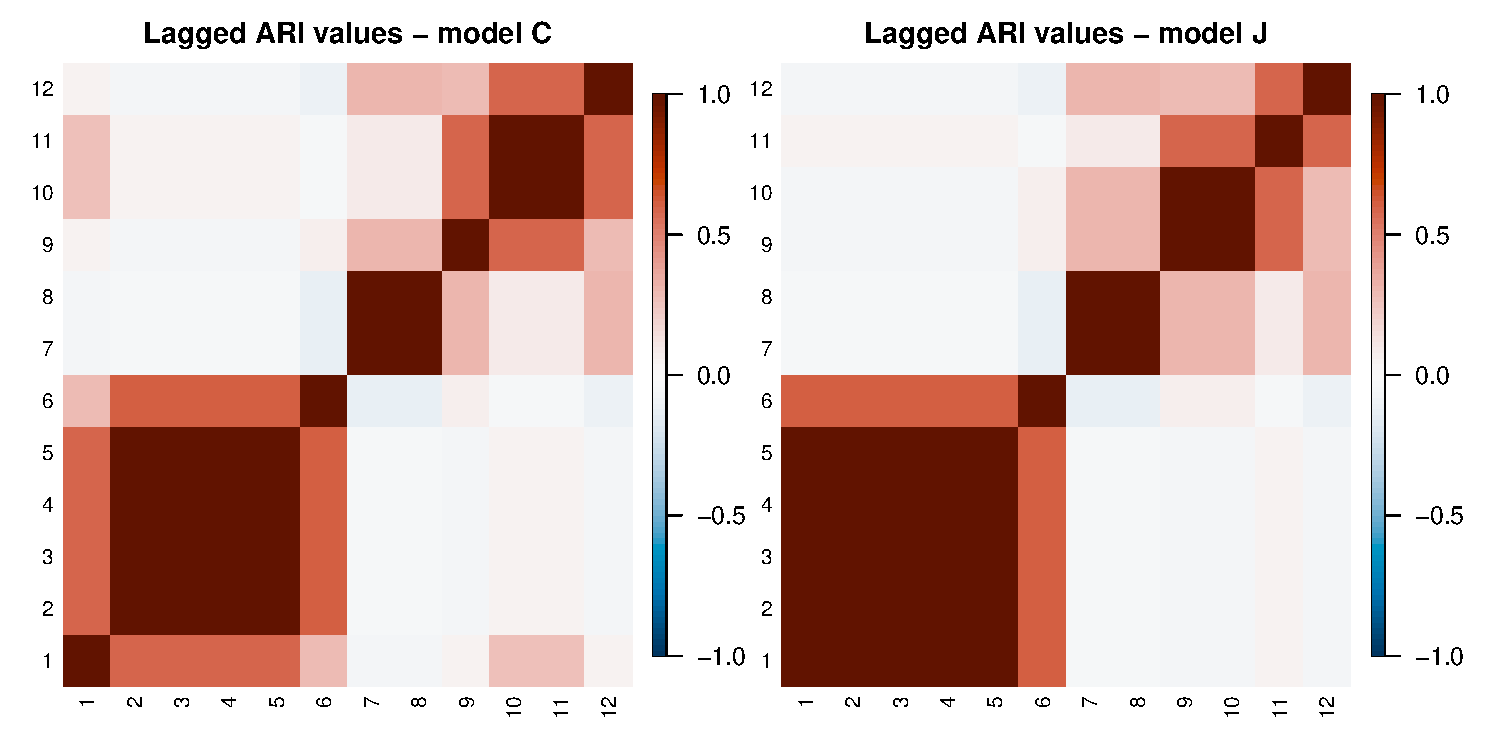
\includegraphics[width=1\linewidth]{Testing/Assessing correctness/no space/ari.pdf}
    \caption[Lagged ARI values of CDRPM and JDRPM fits, target values only]{Lagged ARI values for the two models, on the fit with target only data. The partitions were estimated using the \mjline{salso} function from the corresponding R library.}
    \label{fig:ari no space}
\end{figure}


At this testing stage there were just the target values from $Y_{it}$ to dictate the clusters definition, and both models managed to provide good fits, as we can read from Table \ref{tab: fits metrics no space}. The JDRPM model had better fit metrics (lower WAIC and higher LPML) and also faster execution time, which is however not really relevant in this small-sized fit. Regarding the fitted values, displayed in Figure \ref{fig: fitted and target values no space} together with the original data, they turned out to be also more precise than the one generated by CDRPM, having lower mean squared errors.

\begin{figure}[!htb]
    \centering
    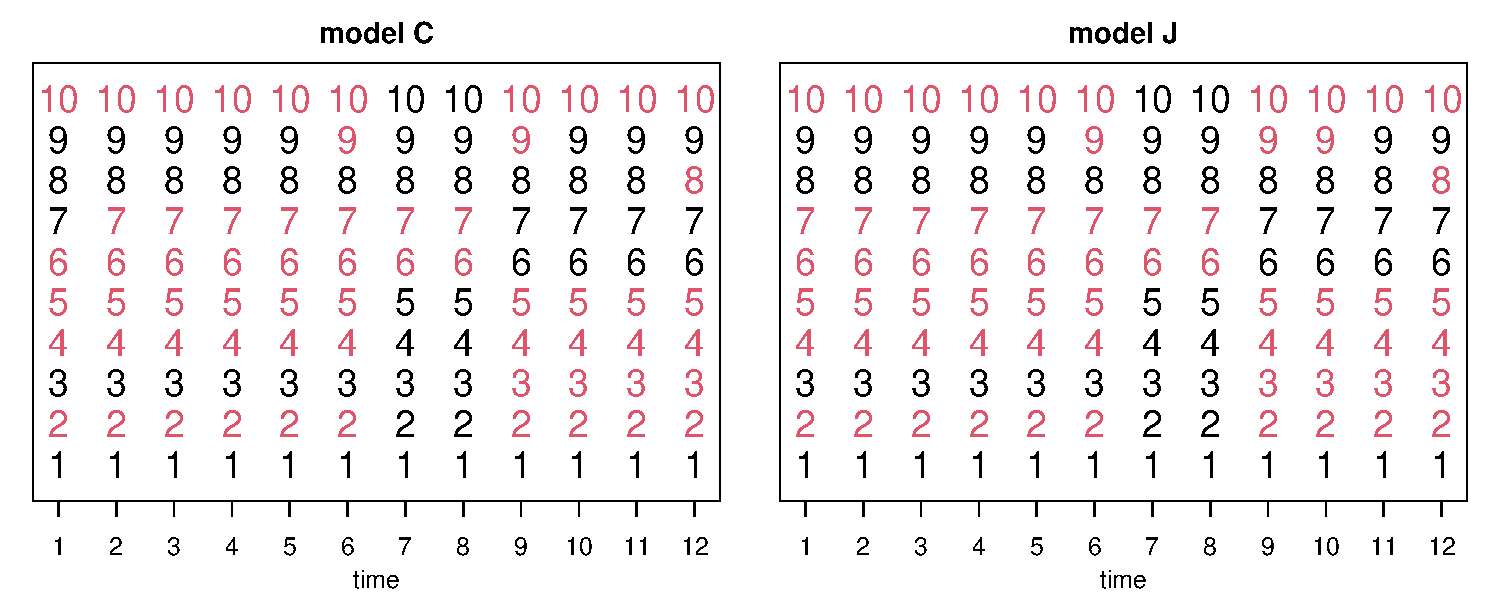
\includegraphics[width=1\linewidth]{Testing/Assessing correctness/no space/partizioni_nums.pdf}
    \caption[Clusters produced by JDRPM and CDRPM fits, target values only]{Clustering produced by the two models, with time points on the $x$ axis, units indicated vertically by their number, and colors representing the cluster label.}
    \label{fig:partizioni no space}
\end{figure}
\begin{figure}[!htb]
    \centering
    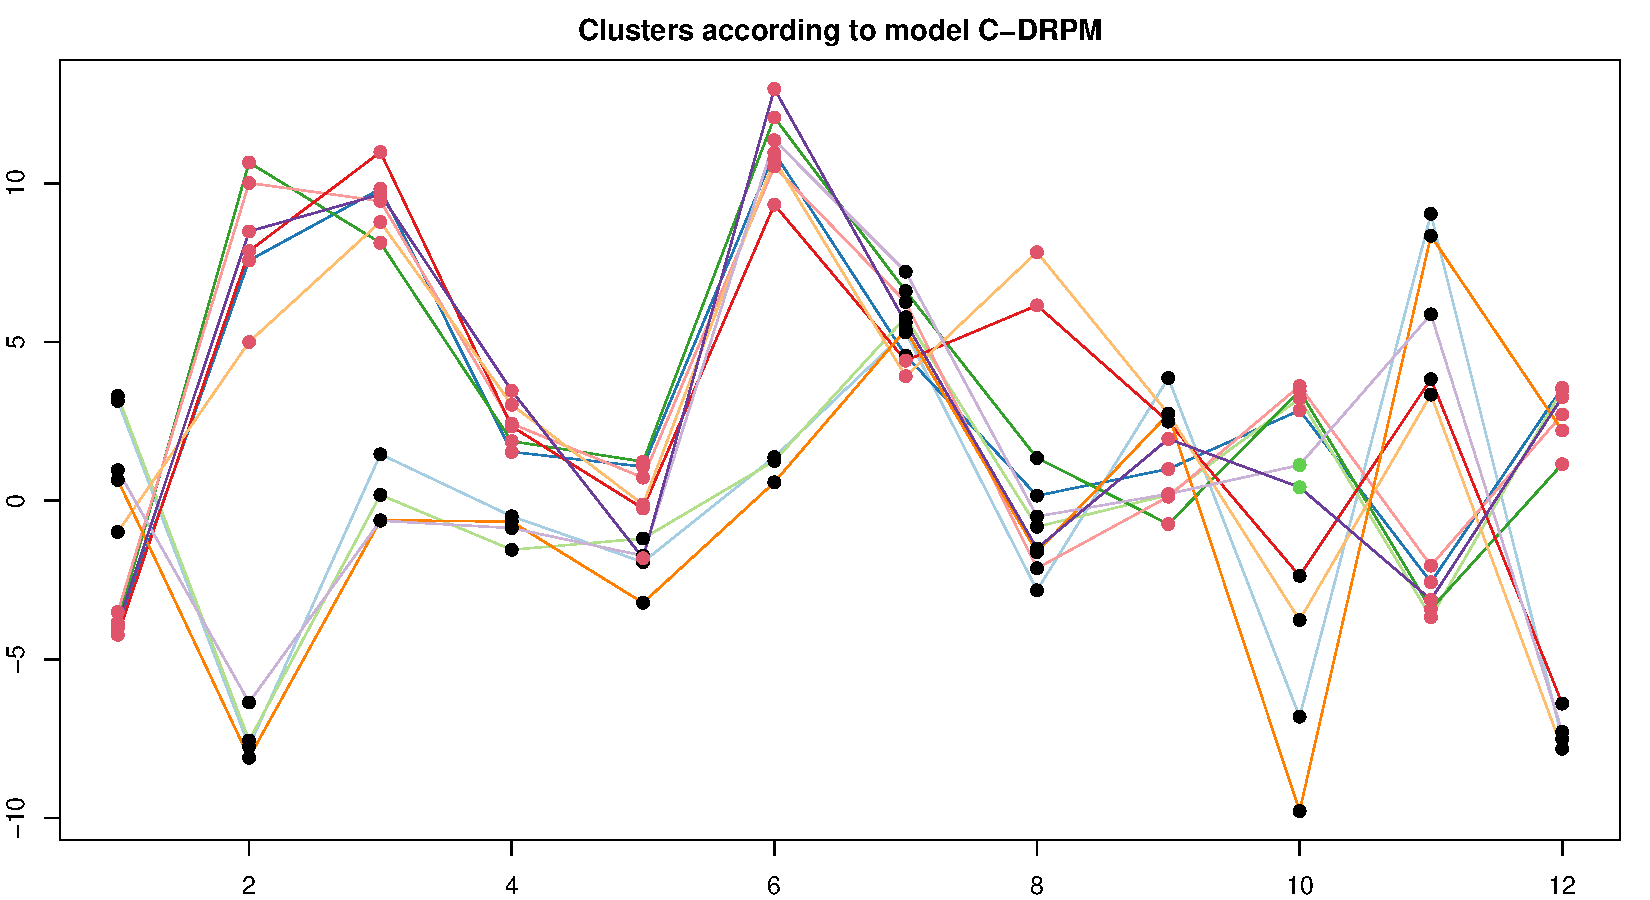
\includegraphics[width=1\linewidth]{Testing/Assessing correctness/no space/clusters_C.pdf}
    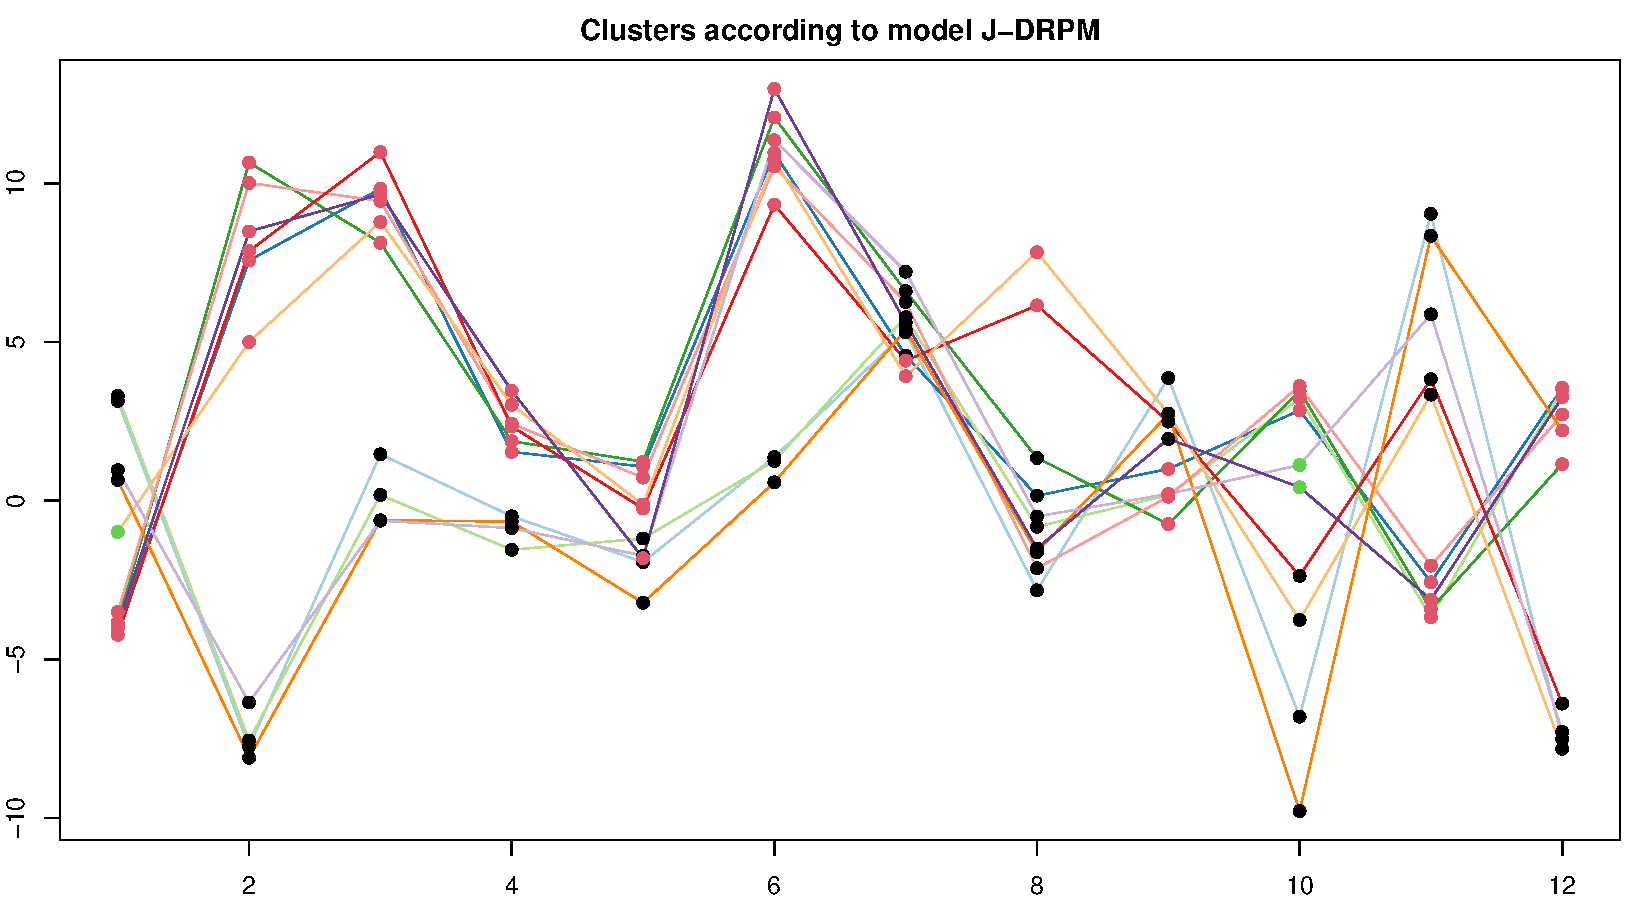
\includegraphics[width=1\linewidth]{Testing/Assessing correctness/no space/clusters_J.pdf}
    \caption[Visual representation of the clusters of JDRPM and CDRPM fits, target values only]{Visual representation of the clusters produced by the models, on the fit with target only data, with units' labels represented as colored dots overlaid to the trend of the generated target variable. The only differences occur at times 1 and 10.}
    \label{fig:clusters no space}
\end{figure}

The resulting clusters were indeed very similar. Figure \ref{fig:ari no space} shows how they manifest the same temporal trend, while Figure \ref{fig:partizioni no space} highlights how the clusters produced are effectively the same except for two differences occurred at times 1 and 10. 
% Although this was a simple test, there is still room for relevant comments. 
By visually inspecting the clusters from Figure \ref{fig:clusters no space}, we can see how at $t=1$ the JDRPM model assigned a red label to a unit closer to the black pack, to which in fact model CDRPM assigned a black label. However, that same unit in the following time instants would be clearly part of the red cluster, thus making the JDRPM choice very reasonable. The opposite happens at $t=10$, where now the CDRPM model seems to give more importance to the temporal trend, assigning a black label to a unit really closer to the red pack but that is destined to enter the black cluster in the following two time instants.



\begin{figure}[!p]
    \centering
    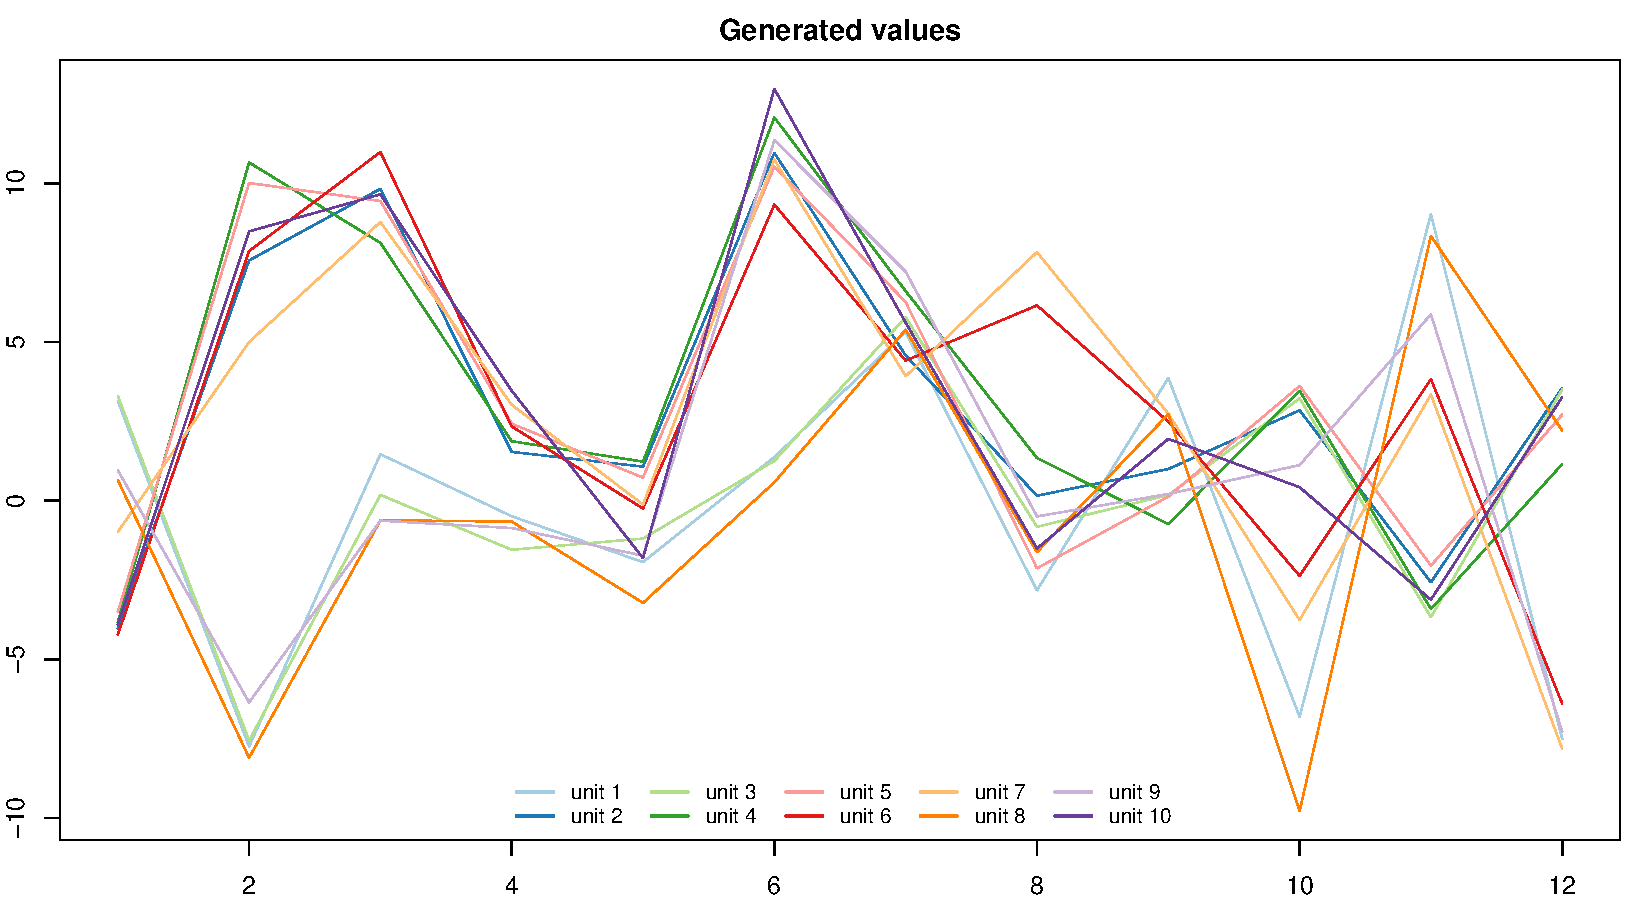
\includegraphics[width=0.97\linewidth]{Testing//Assessing correctness//no space/test_1_generated_data.pdf}
    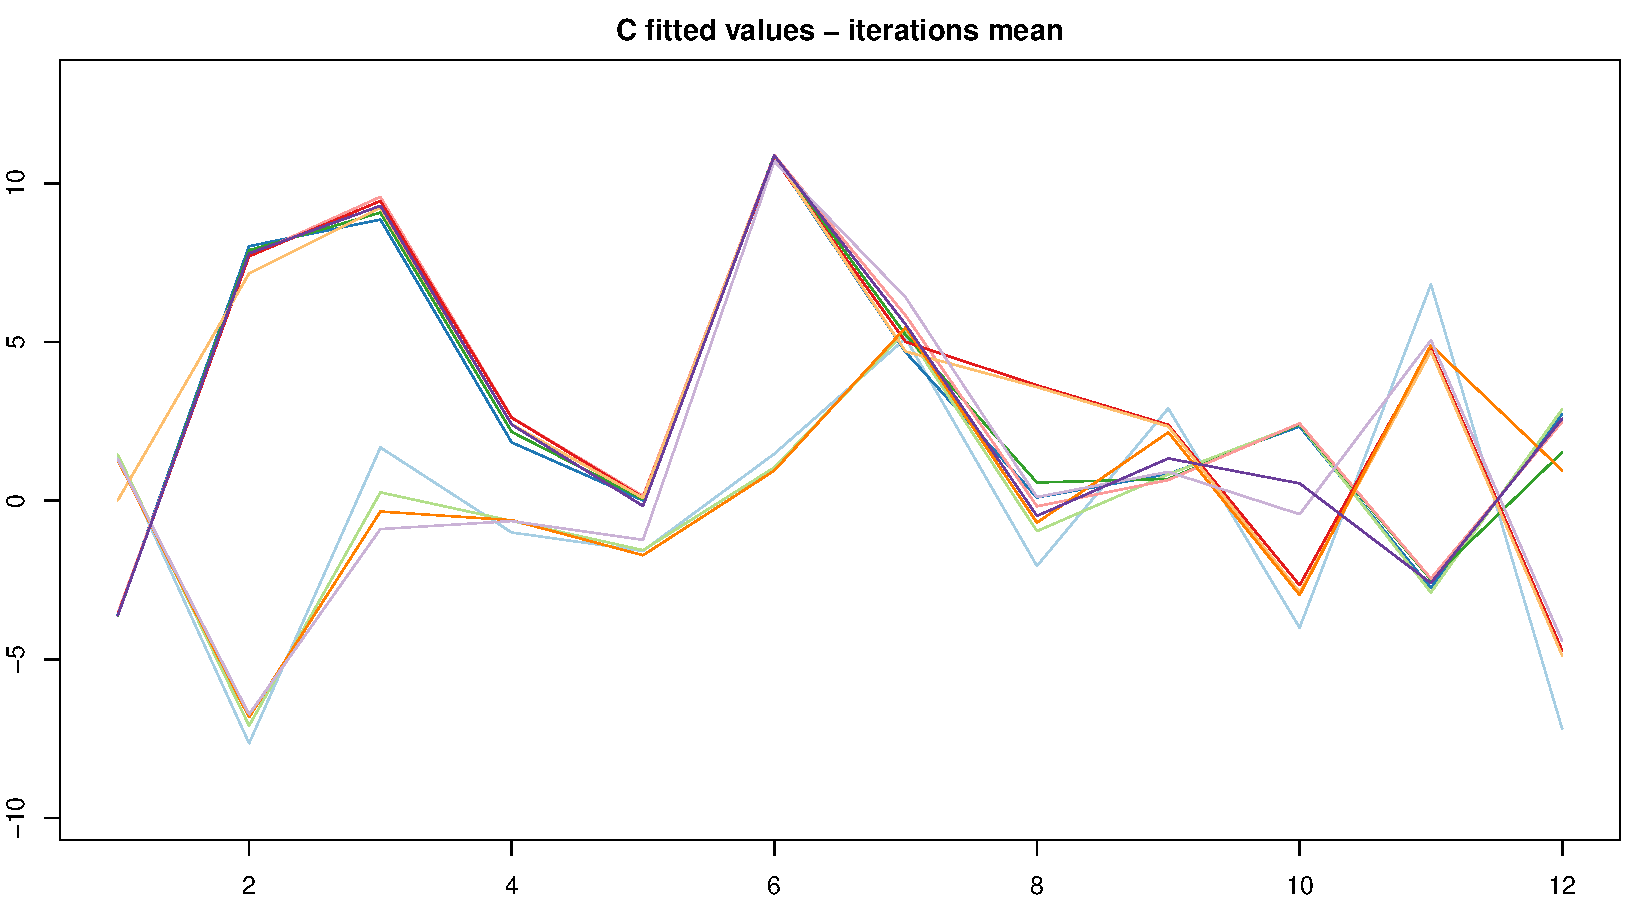
\includegraphics[width=0.97\linewidth]{Testing//Assessing correctness//no space/C_mean_prediction.pdf}
    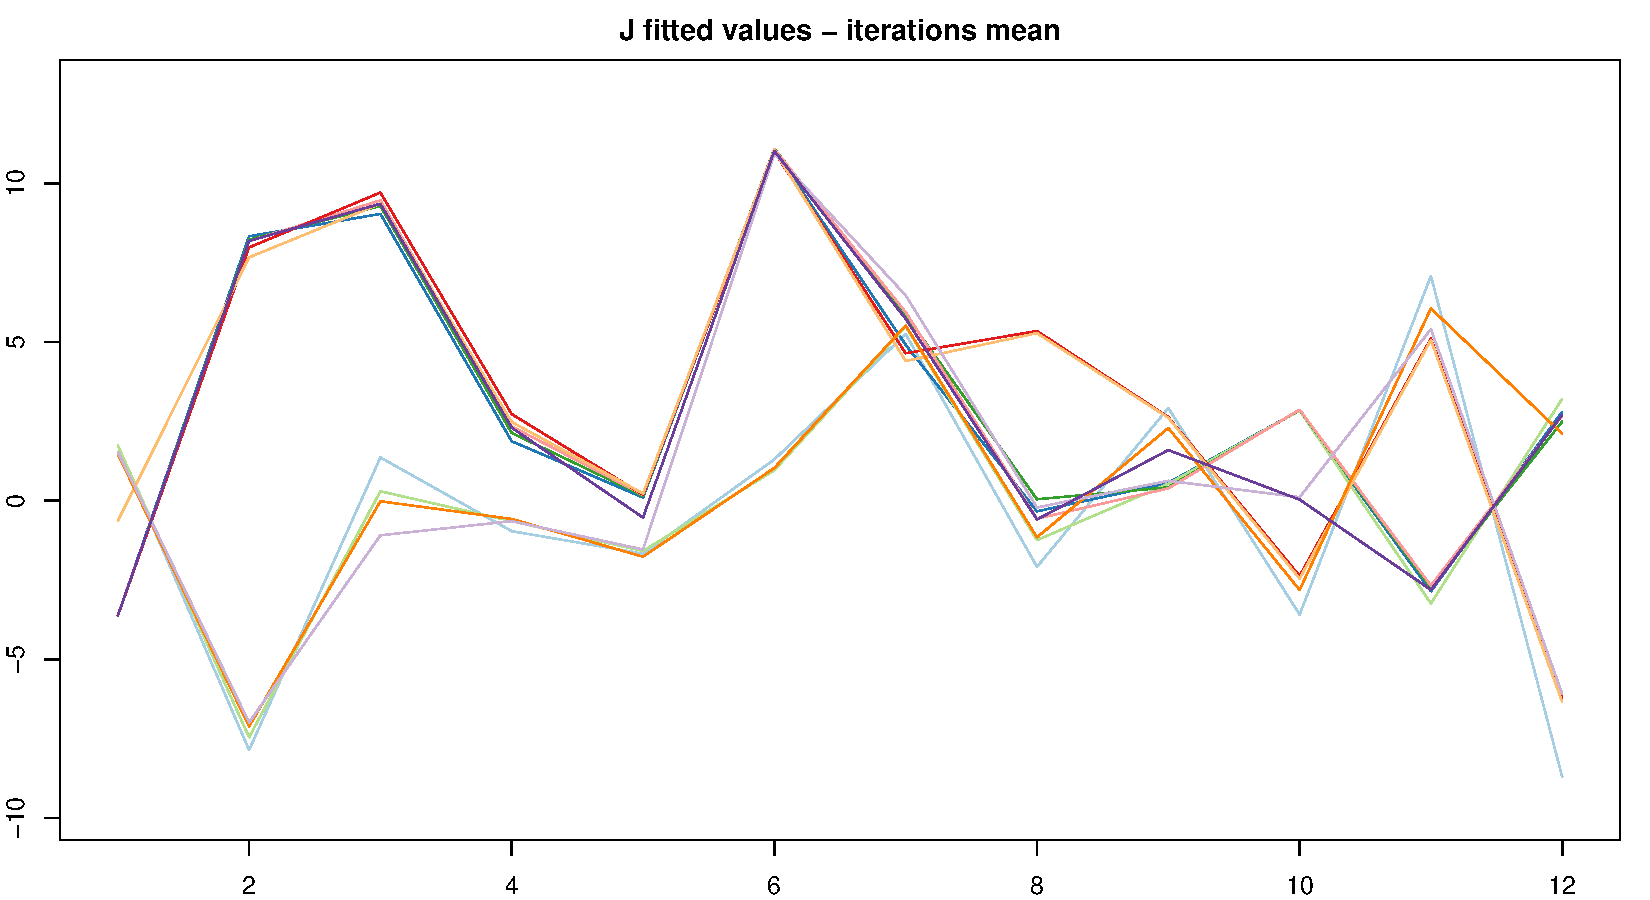
\includegraphics[width=0.97\linewidth]{Testing//Assessing correctness//no space/J_mean_prediction.pdf}
    \caption[Generated and fitted values of JDRPM and CDRPM fits, target values only]{Generated target values (top), together with their fitted values estimate trough the mean of the 1000 iterates generated by model CDRPM (middle) and JDRPM (bottom).}
    \label{fig: fitted and target values no space}
\end{figure}


\subsection{Target variable plus space}
\label{Target variable plus space}
We now consider a more realistic scenario in which we fit the models using a spatio-temporal dataset. In particular, we used the AgrImOnIA \cite{agrimonia} dataset which stores measurements about air pollutants, together with many other environmental variables, in the Lombardy region from 2016 to 2021. For the following testing fits, we employed a summary dataset composed by weekly averages of the data from year 2018. 

\begin{figure}[!ht]
    \centering
    % \includegraphics[width=1\linewidth]{Testing/Covariates/corollary images/WE_tot_precipitationcentered wrt global mean.pdf}
    % \includegraphics[width=1\linewidth]{Testing/Covariates/corollary images/WE_tot_precipitationcentered wrt time-wise mean.pdf}
    \includegraphics[width=1\linewidth]{Testing/Covariates/corollary images/AQ_pm10centered wrt global mean.pdf}
    \includegraphics[width=1\linewidth]{Testing/Covariates/corollary images/AQ_pm10centered wrt time-wise mean.pdf}
    \caption[Comparison of the two possible mean centering methods on the target variable]{Values of the target variable \tt{AQ\_pm10} corrected using the global mean (top) and using the time-wise mean (bottom). This second choice helps to adjust the values range while keeping, or even highlighting, the clustering structural information. Coloring is based on the ranking of $\pmten$ values of the units according to their median, from highest (red) to lowest (blue).}
    \label{fig:different means conceptions PM10}
\end{figure}

The chosen target variable was $\pmten$ whose values had been log-transformed, to recover a normal distribution, and centered with respect to time-wise means. More precisely, each unit $Y_{it}$ was corrected by subtracting the mean $\bar{Y}_t$ of all the observations of that time instant. This procedure, which was the same employed by the authors of the original DRPM during their spatial tests, helps to emphasizes the variations within each time point rather than across the entire dataset. This can be particularly useful to understand how units deviate from their typical behaviour at specific times, potentially highlighting temporal trends and anomalies. This method also removes any temporal bias, e.g. time instants in which all target values were particularly high or low for any particular reason. In contrast, the more traditional choice of centering with respect to the global mean $\bar{Y}$ of the dataset would be useful to just detect global trends, without inspecting deeply into each step. From some test fits performed on the target values with the classical global centering indeed only three clusters appeared, for all time instants. This is of course correct, in some sense, since it's reasonable according to the trend displayed in the top image of Figure \ref{fig:different means conceptions PM10}. However, as we will see shortly, the other version was able to produce several clusters, or at least different partitions at different time instants, improving the specializations of the clusters and the interpretability of the obtained results.

We took all the $n=105$ stations available in the dataset but we limited the time horizon to $T=12$, which corresponds to a three-month monitoring period, just to reduce the time needed to perform all tests. We ran both CDRPM and JDRPM models using the same complete modelling setup, as in Section \ref{Target variable only}, and using a time specific $\alpha$. Convergence was ensured visually by inspecting trace plots and, for the JDRPM model, by numerical diagnostics such as ESS and $\hat R$, which instead the CDRPM model is not able to provide directly from the fit. We collected 4000 iterates, from 110000 total iterates with a burnin of 90000 and thinning by 5. 

\begin{table}[!ht]
    \caption[Accuracy metrics of CDRPM and JDRPM fits, target plus space values]{Summary of the comparison between the two fits on target plus space values. The MSE columns refer to the accuracy between the fitted values generated by the models (estimated by taking the mean and the median of the returned 4000 iterates) and the true values of the target variable. Higher LPML and lower WAIC indicate a better fit.}
    \centering
    \begin{tabular}{cccccc}
    \toprule
          % & \multicolumn{2}{c}{MSE using} & \multicolumn{2}{c}{Fit metrics} & \\
           % \cmidrule(lr){2-3}
           % \cmidrule(lr){4-5}
           & MSE mean &  MSE median & LPML & WAIC & exec. time  \\
           % & mean &  median & LPML & WAIC & execution time  \\
           \midrule
        CDRPM &   0.0142   & 0.0149   & \textbf{ 694.81} & -1768.42 & 1h38m\\
        JDRPM & \textbf{0.0131}  & \textbf{0.0138}   & 624.91 & \textbf{-1898.05}  &  \textbf{48m}\\
        \bottomrule
    \end{tabular}
    \label{tab: fits metrics space}
\end{table}


\begin{figure}[!ht]
    \centering
    \includegraphics[width=1\linewidth]{Testing/Assessing correctness/space/ari.pdf}
    \caption[Lagged ARI values of CDRPM and JDRPM fits, target plus space values]{Lagged ARI values for the two models, on the fit with target plus space data. The partitions were estimated using the \mjline{salso} function from the corresponding R library.}
    \label{fig:ari space}
\end{figure}


\begin{figure}[!p]
    \centering
    \includegraphics[width=0.97\linewidth]{Testing//Assessing correctness//space/test_2_spatial_data.pdf}
    \includegraphics[width=0.97\linewidth]{Testing//Assessing correctness//space/C_mean_prediction.pdf}
    \includegraphics[width=0.97\linewidth]{Testing//Assessing correctness//space/J_mean_prediction.pdf}
    \caption[Target and fitted values of JDRPM and CDRPM fits, target plus space values]{Target $Y_{it}$ values (top), together with their fitted values estimate trough the mean of the 4000 iterates generated by model CDRPM (middle) and JDRPM (bottom).}
    \label{fig: fitted and target values space}
\end{figure}

Table \ref{tab: fits metrics space} shows how both model managed to be accurate not only with respect to the fitting metrics of LPML and WAIC but also in terms of the fitted values. Execution times are also reported, but they are somewhat inaccurate since during the fitting I was busy in writing this thesis, meaning that not all the computational resources of my laptop were devoted to the fitting task. In any case, more precise performance evaluations on the timings will be conducted in Section \ref{chap: Scaling performances}.

From Figure \ref{fig:ari space} we can see how the temporal trend was very similar, confirming again the correctness of the JDRPM implementation. Regarding the similarity of the produced clusters, the partition plot as the one of Figure \ref{fig:partizioni no space} would now be more crowded due to the high number of units. For this reason, in order to still convey that information, we computed $\ari(\rho_{\text{JDRPM}}(t),\rho_{\text{CDRPM}}(t))$ for all time instants $t=1,\ldots,12$, and we obtained a mean of 0.80 and a median of 0.86, denoting high levels of agreement in the clusters produced.

A visual representation of the clusters is provided in Figure \ref{fig:clusters space basic simple}, but will be further detailed and commented in Section \ref{Covariates in the clustering} together with the fits including covariates in the clustering.

\begin{figure}[!p]
    \centering
    \includegraphics[width=1\linewidth]{Testing/Assessing correctness/simple maps/fitCDRPM target + space_simple_map.pdf}
    \includegraphics[width=1\linewidth]{Testing/Assessing correctness/simple maps/fitJDRPM target + space_simple_map.pdf}
    \caption[Clusters generated by CDRPM and JDRPM fits, target plus space values]{Clusters generated by the CDRPM and JDRPM fits with target plus space values.}
    \label{fig:clusters space basic simple}
\end{figure}

% \begin{figure}[!ht]
%     \centering
%     \includegraphics[width=1\linewidth]{Testing/Assessing correctness/space/clusters_C.pdf}
%     \includegraphics[width=1\linewidth]{Testing/Assessing correctness/space/clusters_J.pdf}
%     \caption[Visual representation of the clusters of the JDRPM and CDRPM fits with target plus space values]
% {Visual representation of the clusters produced by the models, on the fit with target plus space data, with units' labels represented as colored dots overlaid to the trend of the target variable.}
%     \label{fig:clusters space}
% \end{figure}



% \begin{figure}[!p]
%     \centering
%     \includegraphics[width=1\linewidth]{Testing/Covariates/corollary images/LA_hvi.pdf}
%     \includegraphics[width=1\linewidth]{Testing/Covariates/corollary images/LA_hvi.pdf}
%     \includegraphics[width=1\linewidth]{Testing/Covariates/corollary images/LA_hvi.pdf}
%     \caption{Enter Caption}
%     \label{fig:enter-label}
% \end{figure}



% \section{Behaviour in presence of missing values}
\section{Performance with missing values}
We now repeat the tests of the previous section on the same datasets but this time with missing values, to see how the JDRPM model reacts to the absence of a full dataset and check if it can still perform well. Based on the amount of missing values in the AgrImOnIA dataset, used for the spatio-temporal tests, we chose to set at 10\% the amount of values that would be replaced by NAs. To perform such replacements, we randomly drew $nT/10$ indexes from the sets $[1,\ldots,n]$ and $[1,\ldots,T]$ to get all the pairs $(i,t)$ which would become missing values in the target variable $Y_{it}$. The dealing of NAs was an upgrade brought by the JDRPM model, so we can't perform these tests with the original CDRPM model since it cannot handle missing data. 

All the following fits have been conducted under the same conditions of their full-dataset counterpart, i.e. using the same models formulation and parameters.

\subsection{Target variable only (NA case)}
The JDRPM seems to exhibit good performance also with missing values. From Table \ref{tab: fits metrics no space julias na full} we can see how the performances, naturally worse than the fit in the full case, are still good. The MSE is inevitably higher since the model did not have all the data points, and so we get less precise fitted values for the corresponding missing spots in the dataset, but the fitted values of Figure \ref{fig: target values estimates no space NA} are still close the one obtained with the fit on full dataset.

\begin{figure}[!ht]
    \centering
    % \includegraphics[width=1\linewidth]{Testing/NA data/no space NA/test_1_generated_data.pdf}
    \includegraphics[width=1\linewidth]{Testing/NA data/no space NA/J_mean_prediction.pdf}
    % \caption{Generated target values (top), together with their fitted values estimate trough the mean of the 1000 iterates generated by model JDRPM (bottom). Special point markers are devoted to the data points corresponding to missing values, to highlight the gaps between the fit on the full dataset and the fit on the NA dataset.}
    \caption[Fitted values of JDRPM fit, target values only, NA dataset]{Fitted values estimate trough the mean of the 1000 iterates generated by model JDRPM. The generated target values were the same of Figure \ref{fig: fitted and target values no space}. Special point markers are used for the data points which were missing, to highlight the gaps between the fitted values on the full dataset (green squares) and the fitted ones on the NA dataset (red squares).}
    \label{fig: target values estimates no space NA}
\end{figure}

From Figures \ref{fig:ari no space NA} and \ref{fig: partizioni no space NA} we can see how we get almost the same temporal trend which we saw in the case without missing data, and indeed the assigned clusters are almost the same. The only difference occurs on a single unit at time 10, where now the JDRPM model does the same thing that CDRPM did in its corresponding fit of Section \ref{Target variable only}. 

\begin{table}[!ht]
    \caption[Accuracy metrics of JDRPM fits, target values only, full vs NA dataset]{Summary of the comparison between the two Julia fits on target values only. The MSE columns refer to the accuracy between the fitted values generated by the models (estimated by taking the mean and the median of the returned 1000 iterates) and the true values of the target variable. Higher LPML and lower WAIC indicate a better fit.}
    \centering
    \begin{tabular}{cccccc}
    \toprule
          % & \multicolumn{2}{c}{MSE using} & \multicolumn{2}{c}{Fit metrics} & \\
           % \cmidrule(lr){2-3}
           % \cmidrule(lr){4-5}
           \textit{JDRPM} & MSE mean &  MSE median & LPML & WAIC & exec. time  \\
           % & mean &  median & LPML & WAIC & execution time  \\
           \midrule
        NA data &   2.1819   & 1.7876 & -239.21 & 417.21 & 3.0s\\
        full data& 1.2628 & 1.2181  & -227.83 & 415.03  &  2.5s \\
        \bottomrule
    \end{tabular}
    \label{tab: fits metrics no space julias na full}
\end{table}


\begin{figure}[!ht]
    \centering
    \includegraphics[width=1\linewidth]{Testing/NA data/no space NA/partizioni_nums.pdf}
    \caption[Clusters produced by JDRPM fits, target values only, full vs NA dataset]{Clustering produced by the two tests on the JDRPM model, with time points on the $x$ axis, units indicated vertically by their number, and colors representing the cluster label.}
    \label{fig: partizioni no space NA}
\end{figure}


\begin{figure}[!ht]
    \centering
    \includegraphics[width=1\linewidth]{Testing/NA data/no space NA/ari.pdf}
    \caption[Lagged ARI values of JDRPM fits, target values only, full vs NA dataset]{Lagged ARI values for the two fits on the JDRPM model with target values only. The partitions were estimated using the \mjline{salso} function from the corresponding R library.}
    \label{fig:ari no space NA}
\end{figure}


\begin{figure}[!ht]
    \centering
    \includegraphics[width=1\linewidth]{Testing/NA data/no space NA/clusters_J.pdf}
    \caption[Visual representation of the clusters of JDRPM fit, target values only, NA dataset]{Visual representation of the clusters produced by the model, with units' labels represented as colored dots overlaid to the trend of the original generated target variables. Special point markers are used for the data points corresponding to missing values.}
    \label{fig:clusters no space NA}
\end{figure}


\subsection{Target variable plus space (NA case)}


\begin{table}[!ht]
    \caption[Accuracy metrics of JDRPM fits, target plus space values, full vs NA dataset]{Summary of the comparison between the two Julia fits on target plus space values. The MSE columns refer to the accuracy between the fitted values generated by the models (estimated by taking the mean and the median of the returned 4000 iterates) and the true values of the target variable. Higher LPML and lower WAIC indicate a better fit.}
    \centering
    \begin{tabular}{cccccc}
    \toprule
          % & \multicolumn{2}{c}{MSE using} & \multicolumn{2}{c}{Fit metrics} & \\
           % \cmidrule(lr){2-3}
           % \cmidrule(lr){4-5}
           \textit{JDRPM} & MSE mean &  MSE median & LPML & WAIC & exec. time  \\
           % & mean &  median & LPML & WAIC & execution time  \\
           \midrule 
        NA data & 0.0160 &  0.0170  &  502.86 & -1793.64 & 43m\\
        full data & 0.0131  & 0.0138   & 624.91 & -1898.05  &  48m \\
        % \midrule
        % & & & & mean & median \\
        % \multicolumn{4}{c}{$\ari(\rho_{\text{JDRPM\_NA}}(t),\rho_{\text{CDRPM\_full}}(t))$} & 1 & 2 \\
        \bottomrule
    \end{tabular}
    \label{tab: fits metrics space julias na full}
\end{table}


\begin{figure}[!ht]
    \centering
    \includegraphics[width=1\linewidth]{Testing/NA data/space/ari.pdf}
    \caption[Lagged ARI values of JDRPM fits, target plus space values, full vs NA dataset]{Lagged ARI values for the two fits on the JDRPM model with target plus space values. The partitions were estimated using the \mjline{salso} function from the corresponding R library.}
    \label{fig: ari space na}
\end{figure}

The JDRPM model seems able to perform well also in the case of fits including spatial information. Table \ref{tab: fits metrics space julias na full} shows how the accuracy reduces, which again is inevitable since we are fitting with missing data, but not drastically. In fact, the drops in LPML and WAIC metrics are just of 3.16\% and 0.95\% respectively. Fitted values are reported in Figure \ref{fig: target values estimates space NA}. Regarding the reported execution times, they are not completely truthful, as already said before, due to the not-full commitment of my laptop resources to the fitting task. In fact, the fit with NA data appeared to be faster than the one with full data, which is somewhat implausible since in the presence of NA data there is the additional load of updating the missing $Y_{it}$ values. Again, more accurate results will be provided in Section \ref{chap: Scaling performances}.

The temporal trend managed as well to remain similar to the trend we saw in Section \ref{Target variable plus space}, as proved by Figure \ref{fig: ari space na}. Regarding the similarity of the produced clusters, we computed the values $\ari(\rho_{\text{JDRPM\_NA}}(t),\rho_{\text{JDRPM\_full}}(t))$ for all time instants $t=1,\ldots,12$, and we obtained a mean of 0.82 and a median of 0.86, denoting still a relatively high level of agreement in the partitions despite the loss of quite some data (121 points out of the 1260 of the full dataset).

\begin{figure}[!ht]
    \centering
    % \includegraphics[width=1\linewidth]{Testing/NA data/no space NA/test_1_generated_data.pdf}
    \includegraphics[width=1\linewidth]{Testing/NA data/space/J_mean_prediction.pdf}
    \caption[Fitted values of JDRPM fit, target plus space values, NA dataset]{Fitted values estimate trough the mean of the 4000 iterates generated by model JDRPM. The generated target values were the same of Figure \ref{fig: fitted and target values space}. Special point markers are used for the data points which were missing, to highlight the gaps between the fitted values on the full dataset (green squares) and the fitted ones on the NA dataset (red squares).}
    \label{fig: target values estimates space NA}
\end{figure}


\section{Effects of the covariates}

\begin{figure}[!ht]
    \centering
    % \includegraphics[width=1\linewidth]{Testing/Covariates/corollary images/WE_blh_layer_maxcentered wrt global mean.pdf}
    % \includegraphics[width=1\linewidth]{Testing/Covariates/corollary images/WE_blh_layer_maxcentered wrt time-wise mean.pdf}
    % \caption[Comparison of the two possible mean centering methods on a covariate]{Values of the \tt{WE\_blh\_layer\_max} covariate corrected using the global mean (top) and using the time-wise mean (bottom). Coloring is based on the ranking of $\pmten$ values of the units according to their median, from highest (red) to lowest (blue).} 
    % \includegraphics[width=1\linewidth]{Testing/Covariates/corollary images/WE_tot_precipitationcentered wrt global mean.pdf}
    % \includegraphics[width=1\linewidth]{Testing/Covariates/corollary images/WE_tot_precipitationcentered wrt time-wise mean.pdf}
    % \caption[Comparison of the two possible mean centering methods on a covariate]{Values of the \tt{WE\_tot\_precipitation} covariate corrected using the global mean (top) and using the time-wise mean (bottom). Coloring is based on the ranking of $\pmten$ values of the units according to their median, from highest (red) to lowest (blue).}
    % \label{fig:different mean correection covariate blh}
    \includegraphics[width=1\linewidth]{Testing/Covariates/corollary images/WE_rh_meancentered wrt global mean.pdf}
    \includegraphics[width=1\linewidth]{Testing/Covariates/corollary images/WE_rh_meancentered wrt time-wise mean.pdf}
    \caption[Comparison of the two possible mean centering methods on a covariate]{Values of the \tt{WE\_rh\_meancentered} covariate corrected using the global mean (top) and using the time-wise mean (bottom). Coloring is based on the ranking of $\pmten$ values of the units according to their median, from highest (red) to lowest (blue).}
    \label{fig:different mean correection covariate blh}
\end{figure}

To perform the fits that will now follow, all the included covariates were treated in the same way as the target value, with the time-wise centering procedure and reasoning described in Section \ref{Target variable plus space}. Figure \ref{fig:different mean correection covariate blh} provides an exemplification of the effect of this transformation on one of the covariates.
Again, this was performed in order to remove any trend or bias on the covariates and to equalize their contribution at each time instant.

We will now see some testing fits which employ the core advancement of the JDRPM update, i.e. the inclusion of covariates. Being with radically different purposes, we will distinguish the cases of covariates in the likelihood and covariates in the clustering. 

\subsection{Covariates in the likelihood}
\label{Covariates in the likelihood}
% \subsubsection{Including covariates in the likelihood}
Continuing on the line of the previous section, we can test if the insertion of covariates in the likelihood can help to recover some accuracy in the case of fits with missing data. In fact, the addition of the regression parameter $\vec{\beta}_t$ had the main goal of improving the accuracy of the model when estimating the target values $Y_{it}$, without affecting too much the cluster generation. With that in mind, the most natural use case of such parameter would be when fitting with missing values. 

Indeed, after including one or multiple covariates in the likelihood, and repeating the fit on the NA dataset under the same conditions, apart from this addition, we saw some improvements. To better illustrate them, we also ran the corresponding fit using the same covariates set in the likelihood, but this time on the full dataset. Results are summarized in Table \ref{tab: fits metrics space julias na full xlk} which also includes, as a reference, the results of the previous fits without the regressor component. Again, the execution times have to be taken with a pinch of salt.

\begin{table}[!ht]
    \caption[Accuracy metrics of JDRPM fits, target plus space values, full vs NA dataset, with vs without covariates in the likelihood]{Summary of the comparison between the JDRPM fits, on target plus space values, plus the fits including also covariates in the likelihood. The MSE columns refer to the accuracy between the fitted values generated by the models (estimated by taking the mean and the median of the returned 4000 iterates) and the true values of the target variable. Higher LPML and lower WAIC indicate a better fit.}
    \centering
    \begin{tabular}{cccccc}
    \toprule
          % & \multicolumn{2}{c}{MSE using} & \multicolumn{2}{c}{Fit metrics} & \\
           % \cmidrule(lr){2-3}
           % \cmidrule(lr){4-5}
           \textit{JDRPM} & MSE mean &  MSE median & LPML & WAIC & exec. time  \\
           % & mean &  median & LPML & WAIC & execution time  \\
           \midrule 
        full data & 0.0131  & 0.0138   & 624.91 & -1898.05  &  \textbf{48m} \\
        full data + Xlk & \textbf{0.0112}  & \textbf{0.0113}   & \textbf{778.96} & \textbf{-2029.84}  &  56m \\
        \midrule
        NA data & 0.0160 &  0.0170  &  502.86 & -1793.64 & \textbf{43m}\\
        NA data + Xlk & \textbf{0.0127} &  \textbf{0.0130}  & \textbf{625.81 }& \textbf{1902.74} & 58m\\
        % \midrule
        % & & & & mean & median \\
        % \multicolumn{4}{c}{$\ari(\rho_{\text{JDRPM\_NA}}(t),\rho_{\text{CDRPM\_full}}(t))$} & 1 & 2 \\
        \bottomrule
    \end{tabular}
    \label{tab: fits metrics space julias na full xlk}
\end{table}



\begin{figure}[!ht]
    \centering
    \includegraphics[width=1\linewidth]{Testing/Covariates/NA lk improvement/beta_allsJDRPM - full data + Xlk.pdf}
    \caption[Regression vector of the fit with multiple covariates in the likelihood, full dataset]{Regression vector $\vec{\beta}_t$ for the $p=6$ covariates inserted in the likelihood in the full data spatio-temporal fit test, with time instants $t=1,\ldots,12$ are on the $x$ axis.}
    \label{fig: lk regressor altitude and friends full}
\end{figure}

\begin{figure}[!ht]
    \centering
    \includegraphics[width=1\linewidth]{Testing/Covariates/NA lk improvement/beta_allsJDRPM - NA data + Xlk.pdf}
    \caption[Regression vector of the fit with multiple covariates in the likelihood, NA dataset]{Regression vector $\vec{\beta}_t$ for the $p=6$ covariates inserted in the likelihood in the NA data spatio-temporal fit test, with time instants $t=1,\ldots,12$ are on the $x$ axis.}
    \label{fig: lk regressor altitude and friends NA}
\end{figure}
\begin{figure}[H]
    \centering
    \includegraphics[width=1\linewidth]{Testing/Covariates/NA lk improvement/ari.pdf}
    \caption[Lagged ARI values of JDRPM fit, target plus space values, full vs NA dataset, with covariates in the likelihood]{Lagged ARI values of the two JDRPM fits with target plus space values on the full and NA datasets, with covariates in the likelihood.}
    \label{fig:ari xlk}
\end{figure}


We can see how clearly the insertion of covariates in the likelihood managed to improve all fitting metrics with, as expected, a decrease in the MSEs, especially in the fits with NA data, proving how that insertion can indeed recover some performance in the case of missing values. The regression vectors $\vec{\beta}_t$ displayed good trace plots, represented in Figures \ref{fig: lk regressor altitude and friends full} and \ref{fig: lk regressor altitude and friends NA}, proving the correctness and effectiveness of the implementation. Moreover the values at which the regressors settled seems to be reasonable and interpretable. For example, it is known that higher altitudes implies lower air pollution, due to the nearly absence of emission sources like industries and vehicles, the more intense winds, the lower atmospheric pressure which facilitates the mixing of the air, and so on; and in fact the $\vec{\beta}_t$ component referring to \tt{Altitude} wanders around negative values, indicating a reduction impact on $\pmten$ concentrations. On the other hand, the \tt{LI\_bovine} covariate, which refers to the density of bovines per km$^2$ in the the area of the measuring station, tends to stay around positive values, since indeed the presence of livestock industries contributes to the emission of air pollutants.


Regarding the generated partitions, they remained substantially unchanged, as briefly depicted in Figure \ref{fig:xlk clusters}. The spatio-temporal trend was as well preserved, displayed in Figure \ref{fig:ari xlk}, except for a generally higher dependence in the second part of the time interval, after the same identified "change point" at $t=4$.  


\begin{figure}[!p]
    \centering
    \includegraphics[width=1\linewidth]{Testing/Covariates/NA lk improvement/fitJDRPM - full data + Xlk_simple_map.pdf}
    \includegraphics[width=1\linewidth]{Testing/Covariates/NA lk improvement/fitJDRPM - NA data + Xlk_simple_map.pdf}
    \caption[Clusters generated by JDRPM fits, target plus space values, full vs NA dataset, with covariates in the likelihood]{Clusters generated by the two JDRPM fits, with target plus space values, on the full and NA datasets, with covariates in the likelihood.}
    \label{fig:xlk clusters}
\end{figure}

The JDRPM fitting function also includes a \mjline{beta_update_threshold} argument, defaulted to zero, to set after which iteration the algorithm should start to update the $\vec{\beta}_t$ parameter. This was an harmless and simple addition, which was considered useful to firstly let the model update and improve the more delicate and relevant parameters for the clustering, such as $\mu^\star_{jt}$ and $\sigma^{2\star}_{jt}$, and secondly tune also the less impactful $\vec{\beta}_t$. Otherwise, maybe, the initial development of the model parameters and clusterings could be biased by early inaccurate samples of the likelihood regressor.  


\begin{figure}[!ht]
    \centering
    % \includegraphics[width=1\linewidth]{Testing/Covariates/NA lk improvement/test_2_spatial_data.pdf}
    \includegraphics[width=1\linewidth]{Testing/Covariates/NA lk improvement/J_mean_prediction_NA.pdf}
    % \includegraphics[width=1\linewidth]{Testing/Covariates/NA lk improvement/J_mean_prediction_full.pdf}
    \caption[Target and fitted values of JDRPM fits, target plus space values, NA dataset, with covariates in the likelihood]{Target and fitted values of the JDRPM fits with target plus space values, on the NA and full dataset, to see the effects of the insertion of covariates in the likelihood.}
    \label{fig: all NA fitted values tests}
\end{figure}

\begin{figure}[!ht]
    \centering
    \includegraphics[width=1\linewidth]{Testing/Covariates/NA lk improvement/trace_plots_with_Xlk.pdf}
    \caption[Trace plot of the fitted values for a fit with covariates in the likelihood]{Example of a trace plot of the fitted values, on a problematic unit $i$ and time instant $t$, comparing the JDRPM fit with covariates in the likelihood to the base (target plus space) CDRPM fit. The green line represents the true value of $Y_{it}$.}
    \label{fig: trace plot with Xlk}
\end{figure}


Finally, Figure \ref{fig: all NA fitted values tests} encloses the fitted values of NA run with covariates in the likelihood. We can see how indeed, visually but also as proved by the better MSEs, these fitted values resemble more the ones of the original target variable, especially if compared to the case of Figure \ref{fig: fitted and target values space}, in which both fits were without any "external suggestion" of covariates in the likelihood. A further proof of this insertion is given by Figure \ref{fig: trace plot with Xlk}, representing the trace plot of the fitted values for a problematic unit and time instant, with problematic in the sense that both the standard JDRPM and CDRPM fits didn't manage to provide precise estimates, which now became more accurate. In the end, this analysis denotes how the addition of this regression parameter $\vec{\beta}_t$ could be beneficial to recover more accuracy in the results, and also help the clustering process since the regressor contribution manifests when using variables computed from the target values inside the update steps of the parameters.  

\subsection{Covariates in the clustering}
\label{Covariates in the clustering}

Now we consider the more theoretically effective and impactful inclusion of covariates in the clustering process. For the choice of which covariates to include, we reasoned about which where the aspects that could affect more the $\pmten$ concentrations, and we ended up selecting the following three covariates:
\begin{itemize}
    \item \tt{WE\_wind\_speed\_10m\_max}. Wind speed plays a significant role in the concentration levels of air pollutants. Its effect is of dual: wind can disperse the pollutants away from their source, spreading them to different areas and thus locally reducing the levels, but it can also have an opposite effect, increasing the amount of contaminants in the air by resuspending the particles which were settled down on the earth surface, such as roads, soils, or buildings. This latter effect is particularly visible in dry and windy rural areas, of which Lombardy is a suitable example. The dataset offered also the wind speed at 100m, but this would be relevant for a wider analysis, where e.g. the trend of $\pmten$ concentrations are followed over multiple regions or countries. Our setup, as with the time-wise mean adjustment, was instead more focused on local and particular behaviours, on the more the ground-level perspective about Lombardy cities.
    
    \item \tt{WE\_tot\_precipitation}. It is well known how rainwater can improve the air quality thanks to water droplets that attract aerosol particles, taking them away from the air, and bringing them to the ground. This process, known as wet deposition, precipitation, scavenging, or washout is indeed very effective in reducing the concentrations of air pollutants. 

\begin{figure}[!p]
    \centering
    \includegraphics[width=1\linewidth]{Testing/Covariates/in clustering/covariate usate/WE_wind_speed_10m_max.pdf}
    \includegraphics[width=1\linewidth]{Testing/Covariates/in clustering/covariate usate/WE_tot_precipitation.pdf}
    \includegraphics[width=1\linewidth]{Testing/Covariates/in clustering/covariate usate/WE_blh_layer_max.pdf}
    \caption[Variables used for the fit tests with covariates in the clustering]{The three variables used to perform the test fit with covariates in the clustering. Colors are based on the ranking of $\pmten$ values of the units according to their median, from highest (red) to lowest (blue).}
    \label{fig: covariate usate nel fit con covariate cl}
\end{figure}
    
    \item \tt{WE\_blh\_layer\_max}. The boundary layer height (BLH) is another relevant variable in terms of the dispersion of air contaminants. This layer defines the height at which air mixing occurs. Usually air gets colder when rising in the atmosphere; however, there could be some warm air regions on top of colder ones. At this boundary, air is not more able to mix, with the warm layer causing a sort of lid, a covering, which traps the lower cold air, with all the contaminants, below it. This reduces the quality of the air since the pollution builds up and accumulates since it has no way to disperse. This covariate, therefore, records the maximum height at which this problematic layer occurs: the lower the values, the higher we should expect the pollutants concentrations to be.
\end{itemize}




To perform this terminal fit with also covariates in the clustering we used the same parameters setup of the previous fits, meaning the same prior coefficients and MCMC configuration. For the covariates we employed similarity $g_4$, the one with the Normal/Normal-Inverse-Gamma model, where we set $\mu_0 =0$, $\lambda_0=1$, $a_0 = 7.5$ and $b_0 = 2$. These choices were motivated both by experimental tunings and by the standardization of the covariates, whose trend, as effectively illustrated by Figure \ref{fig: covariate usate nel fit con covariate cl}, rarely moves outside the $[-1,1]$ interval.



The results are indeed encouraging, as we can see from Table \ref{tab: fits metrics space all with also Xcl} where all metrics appeared to have improved in this ultimate fit. Even with the inclusion of multiple covariates, i.e. with the risk of their "clustering suggestions" to differ, their contribution can still be appreciated by complementing the partition representation to cluster-specific boxplots of the relevant variables, i.e. the target $\pmten$ plus and three included covariates, in this case. Such a comparison is presented in Figure \ref{fig: summary fits battle}.

\begin{table}[!ht]
    \caption[Accuracy metrics of CDRPM and JDRPM fits, target plus space values, with vs without covariates in the clustering process]{Summary of the comparison between the two fits, on target plus space values, plus also the JDRPM fits including covariates in the clustering process. The MSE columns refer to the accuracy between the fitted values generated by the models (estimated by taking the mean and the median of the returned 4000 iterates) and the true values of the target variable. Higher LPML and lower WAIC indicate a better fit.}
    \centering
    \begin{tabular}{cccccc}
    \toprule
          % & \multicolumn{2}{c}{MSE using} & \multicolumn{2}{c}{Fit metrics} & \\
           % \cmidrule(lr){2-3}
           % \cmidrule(lr){4-5}
           & MSE mean &  MSE median & LPML & WAIC & exec. time  \\
           % & mean &  median & LPML & WAIC & execution time  \\
           \midrule
        CDRPM &   0.0142   & 0.0149   &  694.81 & -1768.42 & 1h38m\\
        JDRPM & 0.0131  & 0.0138   & 624.91 & -1898.05  &  \textbf{48m}\\
        % \midrule
        JDRPM + Xcl & \textbf{0.0126}  & \textbf{0.0135}  & \textbf{677.71} & \textbf{-1969.76}  &  1h20m\\
        % JDRPM t+Xcl+Xlk & 0.0126  & 0.0135  & 742.72 & -1759.15  &  35m\\
        \bottomrule
    \end{tabular}
    \label{tab: fits metrics space all with also Xcl}
\end{table}


We can see how the JDRPM fit with also covariates seemed to have captured a slightly better clustering structure than the two competitors. 

Regarding the highest polluted clusters, CDRPM did not manage to characterize better the stations in the right side of the map, while correctly identifying, as the other models did, the big cluster on the right side mostly spanning on Mantova and Brescia areas. The middle-level polluted cluster, which encloses the mountain area was also accurately recovered, similarly to what the JDRPM plus covariates fit did. This cluster seems in fact to be characterized by the lowest level of \tt{WE\_wind\_speed\_10m\_max}. In contrast, the corresponding covariate boxplot in the JDRPM standard fit seems to be more oriented towards higher values. This improvement of a a more reasonable cluster could have been ascribed to the contribute of covariates into the clustering. 

Regarding the lowest polluted cluster, CDRPM decided to separate it into a singleton, while both JDRPM fits decided to keep it into another cluster, therefore causing the appearance of an outlier in the boxplots. As this unit belongs to a mountain region, the inclusion of the \tt{Altitude} covariate could have possibly helped to improve her cluster assignment. Nonetheless, this testing fit seems to provide a confirmation of the potential effectiveness and functionality of the insertion of covariates. The summary representation of the clusters of the JDRPM plus covariates fit is also available in Figure \ref{fig:simple map Jxcl}.


\begin{figure}[!ht]
    \centering
    \includegraphics[width=1\linewidth]{Testing/Covariates/in clustering/space C/CDRPM target + space_t09.pdf}
    \includegraphics[width=1\linewidth]{Testing/Covariates/in clustering/space J/JDRPM target + space_t09.pdf}
    \includegraphics[width=1\linewidth]{Testing/Covariates/in clustering/space J Xcl/JDRPM target + space + Xcl_t09.pdf}
    \caption[Comparison of the clusterings provided by the base fits plus JDRPM with covariates in the clustering]{Comparison of the clusterings provided by the three main models under our analysis: CDRPM and JDRPM with target plus space values, and JDRPM plus with also covariates included in the clustering.}
    \label{fig: summary fits battle}
\end{figure}


\begin{figure}[!ht]
    \centering
    \includegraphics[width=1\linewidth]{Testing/Covariates/in clustering/space J Xcl/fitJDRPM target + space + Xcl_simple_map.pdf}
    \caption[Clusters generated by JDRPM fit, target plus space values, with covariates in the clustering process]{Clusters generated by the JDRPM fit, on target plus space values, with covariates in the clustering process.}
    \label{fig:simple map Jxcl}
\end{figure}


The effect of the insertion of covariates is also proved by Figures \ref{fig: C wind max sorted by cl} and \ref{fig: JXcl wind max sorted by cl}, where we compare the distribution of the clusters with respect to one of the covariate, \tt{WE\_wind\_speed\_10m\_max} in the case of the proposed figure. All the fits had of course the usual $\pmten$ variable as target, meaning that the highest separation should appear there, but we could expect that, with the insertion of covariates, a clustering pattern should also emerge slightly in the auxiliary covariates included. Indeed, the distribution of the clusters in the JDRPM fit with covariates shows a sharper division with respect to the wind speed variable; a division that appears more fuzzy in the CDRPM fit. Also with respect to the JDRPM without covariates of Figure \ref{fig: J wind max sorted by cl} we can see a minor improvement, which could have been probably more significant in the case of datasets without an already-quite clear division in the target variable, since in any case the standard fits of target plus space values were already quite good, in terms of fitting metrics and clusters interpretation.


\begin{figure}[!ht]
    \centering
    \includegraphics[width=1\linewidth]{Testing/Covariates/in clustering/space C/WE_wind_speed_10m_max_sorted.pdf}
    \caption[CDRPM standard fit, clusters distribution with respect to the wind speed covariate]{Distribution of the clusters according to the JDRPM standard fit, with respect to the wind speed covariate. The indication "sorted by clusters" indicates that the order of the units in the plot is based on their cluster membership and not on their original numbering $1,\ldots,n$.}
    \label{fig: C wind max sorted by cl}
\end{figure}


\begin{figure}[!ht]
    \centering
    \includegraphics[width=1\linewidth]{Testing/Covariates/in clustering/space J Xcl/WE_wind_speed_10m_max_sorted.pdf}
    \caption[JDRPM fit with covariates, clusters distribution with respect to the wind speed covariate]{Distribution of the clusters according to the JDRPM fit with covariates, with respect to the wind speed covariate.}    \label{fig: JXcl wind max sorted by cl}
\end{figure}

\begin{figure}[!ht]
    \centering
    \includegraphics[width=1\linewidth]{Testing/Covariates/in clustering/space J/WE_wind_speed_10m_max_sorted.pdf}
    \caption[JDRPM standard fit, clusters distribution with respect to the wind speed covariate]{Distribution of the clusters according to the JDRPM standard fit, with respect to the wind speed covariate.}
    \label{fig: J wind max sorted by cl}
\end{figure}


\section{Scaling performances}
\label{chap: Scaling performances}

To really assess if the goal of faster fits was reached, we setup several tests to compare the two models and the different information levels at which they could be called. The original CDRPM allowed to perform clustering using just the target values or by also including spatial information. In addition to them, the options introduced by JDRPM are the inclusion of covariates at clustering and/or likelihood levels. 

Apart, of course, from the target values, all the other information levels are indeed independent: one could perform the fit ignoring space and accounting just for covariates, for example; but with an additive perspective in mind we decide to perform incremental tests, adding new layers on top of the base ones. Therefore, in what follows, we will see comparisons of fits using just the target values, then those plus space, then those two plus covariates in the clustering, and finally all those plus covariates in the likelihood.

As it appeared from Section \ref{Implementation and optimizations}, the Julia implementation seemed to be a little more eager for memory than the C one. This meant that when we ran the larger tests my system could have ran out of RAM memory, resulting in some data needing to be stored in the slower swap space on the disk, and therefore losing performance. However, on newer or just more technical-oriented machines than my simple laptop, this memory limitation should not be an issue.
% questa parte dopo non è troppo vera, i fit veloci sono comunque veloci anche in Julia, quindi l'overhead di comunicazione sembra trascurabilissimo
% Moreover, we have to remember that the Julia code is called from R, where all the tests were performed, using the transmission control protocol (TCP) of the \mjline{JuliaConnectoR} library, rather than direct calls to the compiled source code as it happens when calling C from R. As a result, this indirect connection can also cause some small overhead, due to the extra time and resources consumed by this communication step. This effect could then have altered the especially the really fast fits, which occurred in the smallest tests.

% Accounting all this, we should consider really accurate just the intermediate-values tests, the ones with $n$ or $T$ being 50 or 100, and take with a pinch of salt the two extremes ones of 10 and 250, in which respectively the communication overhead and hardware limitations could have altered a bit the results. Nonetheless, the results are really encouraging.
Accounting all this, in what follows we should consider really accurate just the intermediate-values tests, i.e. the ones with $n$ or $T$ being 10, 50 or 100, and take with a pinch of salt the extreme one of 250, for which my laptop hardware limitations could have concealed the true accurate results. Nonetheless, the analysis is really encouraging for the JDRPM model.

% To give a reference,  is at least what it seems from our tests on . 

The tests were conducted on randomly generated values, according to $n$ and $T$, for the target data $Y_{it}$ and the spatial coordinates $\vec{s}_i$. In this way, we produced a sort of "mesh" of possible fitting parameters, ranging from small number of units and time horizons to larger ones. To record the expected execution time per iteration of each case we ran each fit with a number of iterations inversely proportional to the size of the test, e.g. 10000 iterations for the case $(n,T)=(10,10)$ and 16 iterations for $(n,T) = (250,250)$. This ensured that each fit lasted approximately the same time. Each fit was ran four times, to then save the minimum time observed during those multiple runs. Such practice, common in benchmarking, helps to eliminate bias from the results due to the system computational demands and fluctuations, filtering in this way just the "ideal" execution time in which all the system performance are devoted to that task.

\begin{figure}[!ht]
    \centering
    \includegraphics[width=1\linewidth]{Testing/Scaling possibilities/target.pdf}
    \caption[Execution times of JDRPM and CDRPM fits, target values only]{Execution times, measured in milliseconds per iteration, when fitting the models using just the target values to generate the clusters. On the JDRPM plot (on the right), in brackets, are reported the speedups relative to the CDRPM timings (on the left), where higher values indicate better performance.}
    \label{fig: scaling target}
\end{figure}

\begin{figure}[!ht]
    \centering
    \includegraphics[width=1\linewidth]{Testing/Scaling possibilities/target_space.pdf}
    \caption[Execution times of JDRPM and CDRPM fits, target plus space values]{Execution times, measured in milliseconds per iteration, when fitting the models using the target values plus the spatial information to generate the clusters. On the JDRPM plot (on the right), in brackets, are reported the speedups relative to the CDRPM timings (on the left), where higher values indicate better performance.}
    \label{fig: scaling target space}
\end{figure}

From Figure \ref{fig: scaling target} we can see how the basic fit, with just the target values, perform very quickly in Julia, with peaks even around a 2x speedup. Similar improvements appeared in the case of fits including also the spatial information, as Figure \ref{fig: scaling target space} shows. Therefore, especially looking at the more reliable non-extreme tests, we can confidently claim that the JDRPM implementation is faster than the CDRPM one.

Regarding fits with covariates, we also generated them randomly by creating matrices of dimensions $n\times p \times T$. For these tests, we avoided to treat different values of $p$: the previous figures summarizing the fits up to spatial information were in fact projection of 3d information ($n$, $T$, and execution time), while if we extended the mesh to also account for $p$, the number of covariates, we would have ended up with 4d information, or even 5d if we considered separately clustering and likelihood covariates. Therefore, to keep things tidy and understandable, we just fixed $p=5$ for both cases.

\begin{figure}[!ht]
    \centering
    \includegraphics[width=1\linewidth]{Testing/Scaling possibilities/target_space_covariates.pdf}
    \caption[Execution times of JDRPM fits, target plus space plus covariates]{Execution times, measured in milliseconds per iteration, when fitting the JDRPM model using target values, spatial information, covariates in the clustering level (left), and covariates in both clustering and likelihood levels (right). In brackets are reported the speedups relative to the JDRPM timings of the fitting with target and space, with higher values still indicating better performance.}
    \label{fig: scaling target space covariates}
\end{figure}


Figure \ref{fig: scaling target space covariates} shows how fits including covariates saw a drop of performance, which was inevitable due to the additional work to perform, but they still remain at a good performance level. Indeed, Figure \ref{fig: summary performance scaling} will point out how some of the fits with all information levels in Julia were actually faster than the basic fits in C.

We can also notice how with larger fits the performance drop reduces to just around 0.8x, rather than the 0.6x of the small cases: this indicates that on fits with heavy $n$ and $T$ the bottleneck is no more the algorithm complexity, meaning the choice of which information levels to include in the clusters generation, but rather the available hardware resources.



\begin{figure}[!ht]
    \centering
    % \includegraphics[width=1\linewidth]{Testing/Scaling possibilities/summary_performance.pdf}
    \includegraphics[width=1\linewidth]{Testing/Scaling possibilities/summary_performance_higher.pdf}
    \caption[Visual representation of all fitting performances]{Visual representation of the performance of all the fits, for all the $n$ and $T$ cases, relatively to the JDRPM fit using target values and spatial information. Namely, the execution time per iteration metric of that fit has been taken as a reference, to which then all other fits have been compared to derive their speedup (or slowdown) factor. Points above the reference line indicate slower fits, while points below denote faster fits.}
    \label{fig: summary performance scaling}
\end{figure} 




\chapter{Conclusion}
\label{chap: conclusion}
% \epigraph{\itshape \flushright
% Honestly, I thought that I would be dead by now (wow)
% }{--- Billie Eilish, \textit{bury a friend}}

% \setlength\epigraphwidth{0.6\textwidth}
\setlength\epigraphwidth{0.6\textwidth}
\epigraph{\itshape
And what in human reckoning seems still afar off, may by the Divine ordinance be close at hand, on the eve of its appearance. And so be it, so be it!
% And what to a man may appear infinitely remote, may in God’s design be very near, already within reach. So it shall be and so be it!”
}{--- F\"{e}dor Dostoevskij, \textit{Brothers Karamazov}}
\setlength\epigraphwidth{0.8\textwidth}

In the end, we can confidently assert that the JDRPM model is a valid improvement of the original DRPM formulation. 

From a theoretical point of view, it offers the same base structure, just with the addition of a possible regression term in the likelihood, while possibly enhancing the quality of the sampled values of the parameters trough the change in the law of the variances from uniform to inverse gamma. In fact, this choice recovers conjugacy in the model and therefore improves the mixing of the chain during the fitting of the model. Plus, of course, the insertion of covariates in the clustering should provide even more accurate results in the generation of the partitions with respect to only having the spatio-temporal information layers.

A possible drawback, inevitable with the increased model complexity, could be the tuning of the parameters, especially in the cohesion and similarity functions to find the right balance between the different contributes of the information levels. However, in this regards, an hopefully helpful analysis was conducted in Chapter \ref{cap: description of the model}, where the effects of the tuning parameters for all cohesions and similarities have been explored. Moreover, the Julia \mjline{MCMC_fit} function provides an optional argument \mjline{cv_weight}, defaulted to 1, which can be used to scale up (or down) the contribute of the covariates similarities, e.g. to make them closer to the interval to which the spatial cohesions values belong. 

This higher complexity appeared also in the tuning of the $\invgamma(a,b)$ parameters, which are indeed more delicate than a simple $\U(l,u)$. To this end, a possible solution could be to run an initial fit with the original CDRPM model, to see where the values of the variances tend to settle, and according to that fixing the $\invgamma$ parameters. For example, in the spatio-temporal tests of Section \ref{Target variable plus space} we saw, from the CDRPM fits, very low values for the variances parameters and as such we assigned, for $\lambda^2$ and $\tau^2_t$ parameters in the JDRPM model, an $\invgamma(a=1.9, b=0.4)$ which has 90\% of his density in the interval $[0.109151, 1.58222]$. The more relevant $\sigma^{2\star}_{jt}$ parameter had also pretty low values, however on that we attached the more uninformative prior $\invgamma(a=0.01, b=0.01)$ which despite being not always suggested \cite{paper-28-prior-variance} turned out to be fine and very precise, relatively to the sampled "reference" values of CDRPM. In general, an alternative solution, probably less theoretically appealing but possibly effective, could be to truncate the $\invgamma$ laws to a certain region in order to avoid sampling extremely high values, which could happen if uninformative priors get not properly adjusted by the data, and also to resemble more the density of a uniform random variable. This choice can be seamlessly implemented in the Julia code by changing \mjline{rand(InverseGamma(a,b))} to \mjline{rand(truncated(InverseGamma(a,b),l,u))}, with $l$ and $u$ being the lower and upper bounds of the designed truncation interval.

From a computational point of view, the goal of faster fits was also reached, reducing the execution times up to a factor of two with respect to the original implementation. This at the cost of a small increase in the memory requirements which however, nowadays, should not be a big deal. 

A final drawback from the two-tiered implementation is time needed to convert back the results from Julia to R, since the \mjline{juliaGet} function from the \mjline{JuliaConnectoR} package can take up to some minutes, especially in fits where lots of iterations are saved. In any case, this latency becomes quite negligible considering the time saved with respect to the original implementation of the \tt{DRPM} package. 

Regarding some possible further improvements, from the theoretical point of view we can also consider satisfied. The complexity of the original DRPM model was already kind of daunting, and the improvements brought by the JDRPM update surely haven't reduced it, considering all the parameters present in the model and especially the ones regulating the spatial cohesions and covariate similarities which strongly determine the final clusters. Therefore, with this complexity in mind, some room for upgrades is easily available in improving the usability of this model. To this end, the current JDRPM implementation has already some basic logging features, where e.g. some steps of the computations can be saved to a text file and analysed afterwards, but more elaborate profiling and monitoring tools could also be implemented, particularly considering the flexible possibilities offered by Julia. Some ideas could be heuristics or suggestions about how to initialize the parameters according to the dataset at hand, or automatic online tuning of the parameters with the progression of iterations. Additionally, visualization tools could be also comfortably implemented trough the extensive plotting ecosystem of Julia, e.g. to return trace plots directly with the execution, provide live-monitoring the distribution of the sampled parameters, and so on. 

Moreover, considering the advancement in performance, a setup with multiple chains ran in parallel, as most of the lighter bayesian models do, could be introduced. Possible further speedup could also be obtained integrating the GPU, if available, to reduce some load from the CPU. Needless to say, the road could already be paved to perform such integration trough the various packages under the \mjline{JuliaGPU} collection.


% --------------------------------------- %
% 	APPENDIX
% --------------------------------------- %
\appendix
% \newgeometry{left=2cm,right=2cm,bottom=2cm}
% \input{MainMatter/Appendice1}
% \restoregeometry
% \input{MainMatter/Appendice2}

\chapter{Theoretical details}
\label{app: theoretical details}

\section{Extended computations of the full conditionals} 
We propose here the extended computations which allowed to extract the full conditionals presented in Chapter \ref{cap: description of the model}. We report also the model graph to make it quickly accessible as a reference for the laws involved in the following computations.

\begin{figure}[!h]
    % \hspace{-36pt} 
    \centering
     \hspace*{-0.04\linewidth}
\begin{tikzpicture}
\begin{scope}[every node/.style={align=center}]
% \begin{scope}[every node/.style={draw,align=center}]
    \node (Y) at (0,10.5) {
    $Y_{it}\sim \mathcal{N}(\mu_{c_{it}t}^\star+\eta_{1i}Y_{it-1} + \alert{\vec{x}_{it}^T\vec{\beta}_t},\sigma^{2\star}_{c_{it}t}(1-\eta_{1i}^2))$ 
    \\ 
    $Y_{i1} \sim \mathcal{N}(\mu^\star_{c_{i1}1} + \alert{\vec{x}_{i1}^T\vec{\beta}_1},\sigma^{2\star}_{c_{i1}1})$
    };
    \node (eta1) at (3,7) {$\xi_i = \text{Logit$(\tfrac{1}{2}(\eta_{1i}+1)$}) \sim \text{Laplace$(a,b)$}$};
    \node (sigma) at (-6,8) {$\sigma_{jt}^{2\star} \sim \alert{\invgamma(a_\sigma, b_\sigma)}$};
    \node (beta) at (6,8) {\alert{$\vec{\beta}_t \sim \N_p(\vec{b},s^2 I)$}};
    \node (mu) at (-3,7) {$\mu_{jt}^\star \sim \N(\theta_t,\tau_t^2)$};

    \node (tau) at (-4,4) {$\tau^2_t \sim \alert{\invgamma(a_\tau,b_\tau)}$};
    \node (theta) at (3,4) {$\theta_t \sim \N((1-\phi_1)\phi_0 + \phi_1\theta_{t-1},\lambda^2(1-\phi_1^2))$\\$\theta_1 \sim \N(\phi_0,\lambda^2)$};

    % \node (alpha) at (-4,2.5){\color{Gray}$(\alpha \sim \text{Beta}(a_\alpha, b_\alpha))$};
    % \node (internals) at (-6,2.5){\color{Gray}$\begin{pmatrix}\alpha_{(it)} \sim \text{Beta}(a_{\alpha(i)}, b_{\alpha(i)})\\ \gamma_{it}\simind \text{Ber}(\alpha_{(it)})\end{pmatrix}$};
    \node (internals) at (-6.5,2.3){\color{Gray}$\alpha_{(it)} \sim \text{Beta}(a_{\alpha(i)}, b_{\alpha(i)})$\\\color{Gray}$ \gamma_{it}\simind \text{Ber}(\alpha_{(it)})$};

    \node (phi0) at (-3,1){$\phi_0\sim \N(m_0,s_0^2)$};
    \node (phi1) at (1,1) {$\phi_1\sim \U(-1,1)$};
    \node (lam2) at (5,1) {$\lambda^2 \sim \alert{\invgamma (a_\lambda,b_\lambda)}$};

    
\end{scope}
% \begin{scope}[>={Stealth[black]},
\begin{scope}[>={latex[black]},
              % every node/.style={fill=white,circle},
              every edge/.style={draw=black,thick}]
    \path [->] (Y) edge (eta1);
    \path [->] (Y) edge (mu);
    \path [->] (Y) edge (sigma);
    \path [->] (Y) edge (beta);
    
    \path [->] (mu) edge (tau);
    \path [->] (mu) edge (theta);
    
    \path [->] (theta) edge (phi0);
    \path [->] (theta) edge (phi1);
    \path [->] (theta) edge (lam2);
    
    % \path [->] (eta1) edge[bend right=60] node {$1$} (E); 
\end{scope}
\end{tikzpicture}
\end{figure}
% \end{center}


\begin{itemize}

\item update $\sigma^{2\star}_{jt}$
\begin{align*}
% \begin{split}
\text{for $t=1$:}&\\
f(\sigma^{2\star}_{jt}|-) & \propto f(\sigma^{2\star}_{jt}) f(\{Y_{it} : c_{it}=j\}|\sigma^{2\star}_{jt},-) \\
& = \law_{\invgamma(a_\sigma,b_\sigma)}(\sigma^{2\star}_{jt}) \prod_{i\in S_{jt}} \law_{\N(\mu^\star_{c_{it}t} + \vec{x}_{it}^T\vec{\beta}_t,\sigma^{2\star}_{c_{it}1})}(Y_{it})\\
& \propto \left[ \left( \frac{1}{\sigma^{2\star}_{jt}}\right)^{a_\sigma+1} \expp{-\frac{1}{\sigma^{2\star}_{jt}}b} \right] \\ & \cdot\left[  \prod_{i \in S_{jt}} 
\left( \frac{1}{\sigma^{2\star}_{jt}}\right)^{1/2} \expp{-\frac{1}{2\sigma^{2\star}_{jt}}(Y_{it}-\mu^\star_{jt}-\vec{x}_{it}^T\vec{\beta}_t)^2} \right]\\
& \propto \left( \frac{1}{\sigma^{2\star}_{jt}}\right)^{(a_\sigma + |S_{jt}|/2)+1}\expp{-\frac{1}{\sigma^{2\star}_{jt}}\left( b_\sigma + \frac{1}{2}\sum_{i \in S_{jt}}(Y_{it}-\mu^\star_{jt}-\vec{x}_{it}^T\vec{\beta}_t)^2 \right)}\\ 
%
 \implies f(\sigma^{2\star}_{jt}&|-)\propto \text{kernel of a $\invgamma(a_{\postp{\sigma}}, b_{\postp{\sigma}})$ with}\\
a_{\postp{\tau}}&= a_\sigma + \frac{|S_{jt}|}{2} \\
%
b_{\postp{\tau}}&=b_\sigma + \frac{1}{2}\sum_{i \in S_{jt}}(Y_{it}-\mu^\star_{jt}-\vec{x}_{it}^T\vec{\beta}_t)^2 
% \end{split}
\tag{\stepcounter{equation}\theequation}
\end{align*}
\begin{align*}
% \begin{split}
\text{for $t>1$:}&\\
f(\sigma^{2\star}_{jt}|-) & \propto f(\sigma^{2\star}_{jt}) f(\{Y_{it} : c_{it}=j\}|\sigma^{2\star}_{jt},-) \\
& = \law_{\invgamma(a_\sigma,b_\sigma)}(\sigma^{2\star}_{jt}) \prod_{i\in S_{jt}} \law_{\N(\mu^\star_{c_{it}t} +\eta_{1i}Y_{it-1}+ \vec{x}_{it}^T\vec{\beta}_t,\sigma^{2\star}_{c_{it}1})}(Y_{it})\\
& \propto \left[ \left( \frac{1}{\sigma^{2\star}_{jt}}\right)^{a_\sigma+1} \expp{-\frac{1}{\sigma^{2\star}_{jt}}b} \right] \\ & \cdot\left[  \prod_{i \in S_{jt}} 
\left( \frac{1}{\sigma^{2\star}_{jt}}\right)^{1/2} \expp{-\frac{1}{2\sigma^{2\star}_{jt}}(Y_{it}-\mu^\star_{jt}-\eta_{1i}Y_{it-1}-\vec{x}_{it}^T\vec{\beta}_t)^2} \right]\\
& \propto \left( \frac{1}{\sigma^{2\star}_{jt}}\right)^{(a_\sigma + |S_{jt}|/2)+1} \\ &\cdot \expp{-\frac{1}{\sigma^{2\star}_{jt}}\left( b_\sigma + \frac{1}{2}\sum_{i \in S_{jt}}(Y_{it}-\eta_{1i}Y_{it-1}-\mu^\star_{jt}-\vec{x}_{it}^T\vec{\beta}_t)^2 \right)}\\ 
%
 \implies f(\sigma^{2\star}_{jt}&|-) \propto \text{kernel of a $\invgamma(a_{\postp{\sigma}}, b_{\postp{\sigma}})$ with}\\
a_{\postp{\tau}}&= a_\sigma + \frac{|S_{jt}|}{2} \\
%
b_{\postp{\tau}}&=b_\sigma + \frac{1}{2}\sum_{i \in S_{jt}}(Y_{it}-\mu^\star_{jt}-\eta_{1i}Y_{it-1}-\vec{x}_{it}^T\vec{\beta}_t)^2 
\tag{\stepcounter{equation}\theequation}
% \end{split}
\end{align*}


\item update $\mu^\star_{jt}$
\begin{align*}
% \begin{split}
\text{for $t=1$:}&\\
    % \text{prior: } \mu^\star_{jt} & \simind \N(\theta_t,\tau^2_t)\\
    f({\mu}_{jt}^\star|-)&\propto f({\mu}_{jt}^\star)f(\{Y_{it} : c_{it}=j\}|\mu^\star_{jt},-)\\
    &=\law_{\N(\theta_t,\tau^2_t)}(\mu^\star_{jt})\prod_{i\in S_{jt}}\law_{\N(\mu^\star_{c_{it}t}+ \vec{x}_{it}^T\vec{\beta}_t,\sigma^{2\star}_{c_{it}1})}(Y_{it})\\
    &\propto \expp{-\frac{1}{2\tau_t^2}(\mu^\star_{jt}-\theta_t)^2} \expp{-\frac{1}{2\sigma^{2\star}_{jt}}\left( \sum_{i \in S_{jt}} (\mu_{jt}^\star - (Y_{i1}-\vec{x}_{it}^T\vec{\beta}_t))^2 \right)}\\
    &\propto \expp{-\frac{1}{2\tau_t^2}(\mu^\star_{jt}-\theta_t)^2} \expp{-\frac{|S_{jt}|}{2\sigma^{2\star}_{jt}}\left( \mu^\star_{jt} - \frac{\text{SUM}_y}{|S_{jt}|} \right)^2}\\
    &\text{where SUM}_y = \sum_{i \in S_{jt}} Y_{i1}-\vec{x}_{it}^T\vec{\beta}_t\\
\implies f(\mu^\star_{jt}&|-) \propto \text{kernel of a $\N(\mu_{\postp{\mu^\star_{jt}}},\sigma^2_{\postp{\mu^\star_{jt}}})$ with}\\
\sigma^2_{\postp{\mu^\star_{jt}}}&=\frac{1}{\frac{1}{\tau^2_t}+\frac{|S_{jt}|}{\sigma^{2\star}_{jt}}}\\
% \sigma^2_{\postp{\mu^\star_{jt}}}&=1 \bigg/ \left[ \tau^2_t+\frac{|S_{jt}|}{\sigma^{2\star}_{jt}}\right]\\
%
\mu_{\postp{\mu^\star_{jt}}}&=\sigma^2_{\postp{\mu^\star_{jt}}}\left( \frac{\theta_t}{\tau_t^2} + \frac{\text{SUM}_y}{\sigma^{2\star}_{jt}} \right)
\tag{\stepcounter{equation}\theequation}
% \end{split}
\end{align*}
\begin{align*}
% \begin{split}
\text{for $t>1$:}&\\
    f({\mu}_{jt}^\star|-)&\propto f({\mu}_{jt}^\star)f(\{Y_{it}: c_{it}=j\}|\mu^\star_{jt},-)\\
    &=\law_{\N(\theta_1,\tau^2_t)}(\mu^\star_{jt})\prod_{i\in S_{jt}}\law_{\N(\mu^\star_{c_{it}t} +\eta_{1i}Y_{it-1}+ \vec{x}_{it}^T\vec{\beta}_t,\sigma^{2\star}_{c_{it}1})}(Y_{it})\\
    &\propto \expp{-\frac{1}{2\tau_t^2}(\mu^\star_{jt}-\theta_t)^2}\\&\cdot \expp{-\frac{1}{2\sigma^{2\star}_{jt}}\left( \sum_{i \in S_{jt}} \frac{1}{1-\eta_{1i}^2}\left(\mu_{jt}^\star - (Y_{it}-\eta_{1i}Y_{i,t-1}-\vec{x}_{it}^T\vec{\beta}_t)\right)^2 \right)} \\
    &\propto \expp{-\frac{1}{2\tau_t^2}(\mu^\star_{jt}-\theta_t)^2} \expp{-\frac{\text{SUM}_{e2}}{2\sigma^{2\star}_{jt}}\left( \mu^\star_{jt}-\frac{\text{SUM}_y}{\text{SUM}_{e2}}\right)^2}\\
    &\text{where SUM}_y = \sum_{i \in S_{jt}} \frac{Y_{it}-\eta_{1i}Y_{i,t-1}-\vec{x}_{it}^T\vec{\beta}_t}{1-\eta_{1i}^2} \text{, SUM}_{e2} = \sum_{i \in S_{jt}} \frac{1}{1-\eta_{1i}^2}\\
\implies f(\mu^\star_{jt}&|-) \propto \text{kernel of a $\N(\mu_{\postp{\mu^\star_{jt}}},\sigma^2_{\postp{\mu^\star_{jt}}})$ with}\\
\sigma^2_{\postp{\mu^\star_{jt}}}&=\frac{1}{\frac{1}{\tau_t^2}+\frac{\text{SUM}_{e2}}{\sigma^{2\star}_{jt}}}\\
%
\mu_{\postp{\mu^\star_{jt}}}&=\sigma^2_{\postp{\mu^\star_{jt}}}\left( \frac{\theta_t}{\tau_t^2} + \frac{\text{SUM}_y}{\sigma_{jt}^{2\star}} \right)
\tag{\stepcounter{equation}\theequation}
% \end{split}
\end{align*}


\item update $\vec{\beta}_t$
\begin{align*}
% \begin{split}
   \text{for $t=1$:}&\\
 f(\vec{\beta}_t|-) & \propto f(\vec{\beta}_t) f(\{ Y_{1t}, \ldots, Y_{nt}\}| \vec{\beta}_t, -)\\
 & = \law_{\N(\vec{b},s^2 I)}(\vec{\beta}_t) \prod_{i=1}^n \law_{ \N(\mu^\star_{c_{it}t} + \vec{x}_{it}^T\vec{\beta}_t,\sigma^{2\star}_{c_{it}t})}(Y_{it}) \\
 & \propto \expp{-\frac{1}{2}\left[ (\vec{\beta}_t^T -\vec{b})^T \frac{1}{s^2} (\vec{\beta}_t-\vec{b}) \right]}
 \\ & \cdot
 \expp{-\frac{1}{2} \sum_{i=1}^n ( Y_{it}-\mu^\star_{c_{it}t} - \vec{x}_{it}^T \vec{\beta}_t )^2}\\
 & \propto \exp \left\{ -\frac{1}{2} \left[ \vec{\beta}_t^T \left( \frac{1}{s^2}I + \sum_{i=1}^n \frac{\vec{x}_{it}\vec{x}_{it}^T}{\sigma^{2\star}_{c_{it}t}}\right)\vec{\beta}_t \right. \right. \\&- \left. \left. 2\left( \frac{\vec{b}}{s^2} +\sum_{i=1}^n \frac{(Y_{it}-\mu^\star_{c_{it}t})\vec{x}_{it}}{\sigma^{2\star}_{c_{it}t}} \right)\cdot \vec{\beta}_t \right] \right\}\\
 %
 \implies f(\vec{\beta}_t&|-) \propto \text{kernel of a $\N(\vec{b}_\post, A_\post)$ with}\\
 A_\post & = \left( \frac{1}{s^2}I + \sum_{i=1}^n \frac{\vec{x}_{it}\vec{x}_{it}^T}{\sigma^{2\star}_{c_{it}t}}\right)^{-1} \\
\vec{b}_\post & = A_\post \left( \frac{\vec{b}}{s^2} +\sum_{i=1}^n \frac{(Y_{it}-\mu^\star_{c_{it}t})\vec{x}_{it}}{\sigma^{2\star}_{c_{it}t}} \right) \\
\iff f(\vec{\beta}_t&|-) \propto \text{kernel of a $\Ncan(\vec{h}_\post, J_\post)$ with}\\
\vec{h}_\post & = \left( \frac{\vec{b}}{s^2} +\sum_{i=1}^n \frac{(Y_{it}-\mu^\star_{c_{it}t})\vec{x}_{it}}{\sigma^{2\star}_{c_{it}t}} \right) \\
J_\post & = \left( \frac{1}{s^2}I + \sum_{i=1}^n \frac{\vec{x}_{it}\vec{x}_{it}^T}{\sigma^{2\star}_{c_{it}t}}\right)
\tag{\stepcounter{equation}\theequation}
% \end{split}
\end{align*}
\begin{align*}
% \begin{split}
   \text{for $t>1$:}&\\
    f(\vec{\beta}_t|-) & \propto f(\vec{\beta}_t) f(\{ Y_{1t}, \ldots, Y_{nt}\}| \vec{\beta}_t, -)\\
 & = \law_{\N(\vec{b},s^2 I)}(\vec{\beta}_t) \prod_{i=1}^n \law_{ \N(\mu^\star_{c_{it}t} + \eta_{1i}Y_{it-1} + \vec{x}_{it}^T\vec{\beta}_t,\sigma^{2\star}_{c_{it}t})}(Y_{it}) \\
 & \propto \expp{-\frac{1}{2}\left[ (\vec{\beta}_t^T -\vec{b})^T \frac{1}{s^2} (\vec{\beta}_t-\vec{b}) \right]} \\ & \cdot \expp{-\frac{1}{2} \sum_{i=1}^n ( Y_{it}-\mu^\star_{c_{it}t} -  \eta_{1i}Y_{it-1}-\vec{x}_{it}^T \vec{\beta}_t )^2}\\
 & \propto \exp \left\{-\frac{1}{2} \left[ \vec{\beta}_t^T \left( \frac{1}{s^2}I + \sum_{i=1}^n \frac{\vec{x}_{it}\vec{x}_{it}^T}{\sigma^{2\star}_{c_{it}t}}\right)\vec{\beta}_t \right. \right. \\& \left. \left. - 2\left( \frac{\vec{b}}{s^2} +\sum_{i=1}^n \frac{(Y_{it}- \mu^\star_{c_{it}t}- \eta_{1i}Y_{it-1})\vec{x}_{it}}{\sigma^{2\star}_{c_{it}t}} \right)\cdot \vec{\beta}_t \right] \right\}\\
 %
 \implies f(\vec{\beta}_t&|-) \propto \text{kernel of a $\N(\vec{b}_\post, A_\post)$ with}\\
 A_\post & = \left( \frac{1}{s^2}I + \sum_{i=1}^n \frac{\vec{x}_{it}\vec{x}_{it}^T}{\sigma^{2\star}_{c_{it}t}}\right)^{-1} \\
\vec{b}_\post & = A_\post \left( \frac{\vec{b}}{s^2} +\sum_{i=1}^n \frac{(Y_{it}-\mu^\star_{c_{it}t}- \eta_{1i}Y_{it-1})\vec{x}_{it}}{\sigma^{2\star}_{c_{it}t}} \right) \\
 \iff f(\vec{\beta}_t&|-) \propto \text{kernel of a $\Ncan(\vec{h}_\post, J_\post)$ with}\\
\vec{h}_\post & = \left( \frac{\vec{b}}{s^2} +\sum_{i=1}^n \frac{(Y_{it}-\mu^\star_{c_{it}t}- \eta_{1i}Y_{it-1})\vec{x}_{it}}{\sigma^{2\star}_{c_{it}t}} \right) \\
J_\post & = \left( \frac{1}{s^2}I + \sum_{i=1}^n \frac{\vec{x}_{it}\vec{x}_{it}^T}{\sigma^{2\star}_{c_{it}t}}\right)
\tag{\stepcounter{equation}\theequation}
% \end{split}
\end{align*}

\item update $\tau^2_t$
\begin{align*}
% \begin{split}
% \text{prior: } \tau^2_t & \simiid \invgamma(a_\tau, b_\tau)\\
f(\tau^2_t|-) & \propto  f(\tau^2_t) f((\mu^\star_{1t},\ldots,\mu^\star_{k_tt})|\tau^2_t,-)\\
& = \law_{\invgamma(a_\tau,b_\tau)}(\tau^2_t)\prod_{j=1}^{k_t} \law_{\N(\theta_t,\tau^2_t)}(\mu^\star_{jt})\\
&\propto \left[\left( \frac{1}{\tau_t^2}\right)^{a_\tau+1} \expp{-\frac{b_\tau}{\tau^2_t}}\right] \left[ \prod_{j=1}^{k_t} \left( \frac{1}{\tau^2_t}\right)^{1/2}\expp{-\frac{1}{2\tau^2_t}(\mu^\star_{jt}-\theta_t)^2}\right]\\
& \propto \left( \frac{1}{\tau^2_t}\right)^{\left( \frac{k_t}{2}+a_\tau\right)+1} \expp{-\frac{1}{\tau^2_t}\left( \frac{\sum_{j=1}^{k_t}(\mu_{jt}^\star-\theta_t)^2}{2}+b_\tau\right)}\\    
\implies f(\tau^2_t&|-)\propto \text{kernel of a $\invgamma(a_{\postp{\tau}}, b_{\postp{\tau}})$ with}\\
a_{\postp{\tau}}&=\frac{k_t}{2}+a_\tau\\
%
b_{\postp{\tau}}&= \frac{\sum_{j=1}^{k_t}(\mu_{jt}^\star-\theta_t)^2}{2}+b_\tau
\tag{\stepcounter{equation}\theequation}
% \end{split}
\end{align*}
    

\item update $\theta_t$
\begin{align*}
% \begin{split}
    \text{for $t=T$:}&\\
    f(\theta_t|-)&\propto f(\theta_t)f((\mu^\star_{1t},\ldots,\mu^\star_{k_tt})|\theta_t,-)\\
    % =f(\theta_t)\prod_{j=1}^{k_t}f(\mu_{jt}^\star|\theta_t,-)\\
    %
    &=\law_{\N((1-\phi_1)\phi_0 + \phi_1\theta_{t-1},\lambda^2(1-\phi_1^2))}(\theta_t)\prod_{j=1}^{k_t} \law_{\N(\theta_t,\tau^2_t)}(\mu^\star_{jt})\\
    %
    &\propto\expp{-\frac{1}{2(\lambda^2(1-\phi_1^2))}\Big(\theta_t - ((1-\phi_1)\phi_0+\phi_1\theta_{t-1})\Big)^2}\\
    &\cdot \expp{-\frac{k_t}{2\tau^2_t}\left(\theta_t - \frac{\sum_{j=1}^{k_t}\mu^\star_{jt}}{k_t}\right)}\\
    \implies f(\theta_t&|-)\propto \text{kernel of a $\N(\mu_{\postp{\theta_t}},\sigma^2_{\postp{\theta_t}})$ with}\\
    \sigma^2_{\postp{\theta_t}}&=\dfrac{1}{\frac{1}{\lambda^2(1-\phi_1^2)}+\frac{k_t}{\tau_t^2}}\\
    \mu_{\postp{\theta_t}}&=\sigma^2_{\postp{\theta_t}}\left(\frac{\sum_{j=1}^{k_t}\mu^\star_{jt}}{\tau^2_t} + \frac{(1-\phi_1)\phi_0+\phi_1\theta_{t-1}}{\lambda^2(1-\phi_1^2)} \right)
    \tag{\stepcounter{equation}\theequation}
% \end{split}
\end{align*}
\begin{align*}
% \begin{split}
    % \text{for $1<t<T$:}&\\
    \text{for } 1<t&<T\text{:}\\
    f(\theta_t|-)&\propto \underbrace{f(\theta_t)f((\mu^\star_{1t},\ldots,\mu^\star_{k_tt})|\theta_t,-)}_{\text{as in the case $t=T$}} f(\theta_{t+1}|\theta_t,-)\\
    &=\law_{\N( \mu_{\postp{\theta_t}},\sigma^2_{\postp{\theta_t}})}(\theta_t) \law_{\N((1-\phi_1)\phi_0 + \phi_1\theta_{t},\lambda^2(1-\phi_1^2))}(\theta_{t+1})\\
    &\propto\expp{-\frac{1}{2\sigma^2_{\postp{\theta_t}}}\left(\theta_t -\mu_{\postp{\theta_t}}\right)^2}\\& \cdot \expp{-\frac{1}{2\frac{\lambda^2(1-\phi_1^2)}{\phi_1^2}}\left(\theta_t - \frac{\theta_{t+1}-(1-\phi_1)\phi_0}{\phi_1}\right)^2}\\
    \implies f(\theta_t&|-)\propto \text{kernel of a $\N(\mu_{\postp{\theta_t}},\sigma^2_{\postp{\theta_t}})$ with}\\
    \sigma^2_{\postp{\theta_t}}&=\dfrac{1}{\frac{1+\phi_1^2}{\lambda^2(1-\phi_1^2)}+\frac{k_t}{\tau^2_t}}\\
\mu_{\postp{\theta_t}}&=\sigma^2_{\postp{\theta_t}}\left(\frac{\sum_{j=1}^{k_t}\mu^\star_{jt}}{\tau^2_t} + \frac{\phi_1(\theta_{t-1}+\theta_{t+1}) + \phi_0(1-\phi_1)^2}{\lambda^2(1-\phi_1^2)} \right)
    \tag{\stepcounter{equation}\theequation}
% \end{split}
\end{align*}
\begin{align*}
% \begin{split}
    \text{for $t=1$:}&\\
    f(\theta_t|-) &\propto f(\theta_t)f(\theta_{t+1}|\theta_t,-)f(\vec{\mu}^\star_t|\theta_t,-)\\
    %
    &=\law_{\N(\phi_0,\lambda^2)}(\theta_t) \law_{\N((1-\phi_1)\phi_0 + \phi_1\theta_{t-1},\lambda^2(1-\phi_1^2))}(\theta_{t+1})\prod_{j=1}^{k_t} \law_{\N(\theta_t,\tau^2_t)}(\mu^\star_{jt})\\
    %
    &\propto\expp{-\frac{1}{2\lambda^2}(\theta_t-\phi_0)^2}\\&\cdot\expp{-\frac{1}{2\frac{\lambda^2(1-\phi_1^2)}{\phi_1^2}}\left(\theta_t - \frac{\theta_{t+1}-(1-\phi_1)\phi_0}{\phi_1}\right)^2}\\&\cdot \expp{-\frac{k_t}{2\tau^2_t}\left(\theta_t - \frac{\sum_{j=1}^{k_t}\mu^\star_{jt}}{k_t}\right)}\\
    \implies f(\theta_t&|-)\propto \text{kernel of a $\N(\mu_{\postp{\theta_t}},\sigma^2_{\postp{\theta_t}})$ with}\\
    \sigma^2_{\postp{\theta_t}}&=\dfrac{1}{\frac{1}{\lambda^2}+\frac{\phi_1^2}{\lambda^2(1-\phi_1^2)}+\frac{k_t}{\tau^2_t}}\\
\mu_{\postp{\theta_t}}&=\sigma^2_{\postp{\theta_t}}\left(\frac{\phi_0}{\lambda^2}+\frac{\phi_1(\theta_{t+1}-(1-\phi_1)\phi_0)}{\lambda^2(1-\phi_1^2)}+\frac{\sum_{j=1}^{k_t}\mu^\star_{jt}}{\tau^2_t} \right)
\tag{\stepcounter{equation}\theequation}
% \end{split}
\end{align*}


\item update $\phi_0$
\begin{align*}
% \begin{split}
            % f(\phi_0|-) &\propto f(\phi_0) \cdot f(\vec{\theta}_t|\phi_0,\phi_1,\lambda) \\
        f(\phi_0|-) &\propto f(\phi_0) f((\theta_1,\ldots,\theta_T)|\phi_0,-) \\
        %
        &= \law_{\N(m_0,s^2_0)}(\phi_0) \law_{\N(\phi_0,\lambda^2)}(\theta_1) \prod_{t=2}^T \L_{\N((1-\phi_1)\phi_0 + \phi_1\theta_{t-1},\lambda^2(1-\phi_1^2))}(\theta_t)\\
        %
        % &= \L_{\N(m_0,s^2_0)}(\phi_0)\cdot \left[ \L_{\N(\phi_0,\lambda^2)}(\theta_1) \prod_{t=2}^T \L_{\N((1-\phi_1)\phi_0 + \phi_1\theta_{t-1},\lambda^2(1-\phi_1^2))}(\theta_t)\right]\\
        %
        % &= \N(m_0,s^2_0)(\phi_0)\cdot \left[ \N(\phi_0,\lambda^2)(\theta_1) \prod_{t=2}^T \N((1-\phi_1)\phi_0 + \phi_1\theta_{t-1},\lambda^2(1-\phi_1^2))(\theta_t)\right]\\
        %
        &\propto \exp{\left\{-\frac{1}{2s_0^2}(\phi_0-m_o)^2\right\}}\exp{\left\{-\frac{1}{2\lambda^2}(\phi_0-\theta_1)^2\right\}}\\
        & \cdot \exp{\left\{-\frac{1}{2\frac{\lambda^2(1-\phi_1^2)}{(T-1)(1-\phi_1)^2}}\left(\phi_0-\frac{(1-\phi_1)(\text{SUM}_t)}{(T-1)(1-\phi_1)^2}\right)^2\right\}}\\& \text{where SUM}_t = \sum_{t=2}^T(\theta_t-\phi_1\theta_{t-1})\\
    \implies f(\phi_0&|-) \propto \text{kernel of a $\N(\mu_{\phi_0\post},\sigma^{2}_{\phi_0\post})$ with}\\
    \sigma^{2}_{\postp{\phi_0}} &= \dfrac{1}{\frac{1}{s_0^2}+\frac{1}{\lambda^2}+\frac{(T-1)(1-\phi_1)^2}{\lambda^2(1-\phi_1^2)}}\\
    % \mu_{\phi_0\post} &= \sigma^{2}_{\phi_0\post} \left[\dfrac{m_0}{s_0^2}+\dfrac{\theta_1}{\lambda^2}+\dfrac{1-\phi_1}{\lambda^2(1-\phi_1^2)}\left( \sum_{t=2}^T \theta_t-\phi_1\theta_{t-1}\right)\right]
    \mu_{\phi_0\post} &= \sigma^{2}_{\phi_0\post} \left(\dfrac{m_0}{s_0^2}+\dfrac{\theta_1}{\lambda^2}+\dfrac{1-\phi_1}{\lambda^2(1-\phi_1^2)}\text{SUM}_t\right)
\tag{\stepcounter{equation}\theequation}
% \end{split}
\end{align*}

\item update $\lambda^2$
% \begin{equation} \label{eq1}
\begin{align*}
% \begin{split}
    % \text{prior: } \lambda^2 & \simiid \invgamma(a_\lambda, b_\lambda)\\
    f(\lambda^2|-) & \propto  f(\lambda^2) f(\theta_1,\ldots,\theta_T|\lambda^2,-)\\
    & = \law_{\invgamma(a_\lambda,b_\lambda)}(\lambda^2)\law_{\N(\phi_0,\lambda^2)}(\theta_1)\prod_{t=2}^{T} \law_{\N((1-\phi_1)\phi_0 +\phi_1\theta_{t-1},\lambda^2(1-\phi_1^2))}(\theta_t)\\
    &\propto \left[ \left( \frac{1}{\lambda_t^2}\right)^{a_\lambda+1} \expp{-\frac{b_\lambda}{\lambda^2}}\right] \left[ \left(\frac{1}{\lambda^2}\right)^{1/2} \expp{-\frac{1}{2\lambda^2}(\theta_1-\phi_0)^2}\right] \\
    &\cdot \left[ \prod_{t=2}^T \left(\frac{1}{\lambda^2}\right)^{1/2} \expp{-\frac{1}{2\lambda^2}\left( \theta_t - (1-\phi_1)\phi_0 -\phi_1\theta_{t-1}\right)^2} \right]\\
    & \propto \left( \frac{1}{\lambda^2}\right)^{\left( \frac{T}{2}+a_\lambda\right)+1}\\& \cdot\expp{-\frac{1}{\lambda^2}\left( \frac{(\theta_1-\phi_0)^2}{2}
 + \sum_{t=2}^T \frac{\left( \theta_t - (1-\phi_1)\phi_0 -\phi_1\theta_{t-1}\right)^2}{2}+b_\lambda\right)}\\
    %
    \implies f(\lambda^2&|-)\propto \text{kernel of a $\invgamma(a_{\postp{\lambda}}, b_{\postp{\lambda}})$ with}\\
a_{\postp{\lambda}}&=\frac{T}{2}+a_\lambda\\
%
b_{\postp{\lambda}}&=  \frac{(\theta_1-\phi_0)^2}{2}
 + \sum_{t=2}^T \frac{\left( \theta_t - (1-\phi_1)\phi_0 -\phi_1\theta_{t-1}\right)^2}{2}+b_\lambda
 \tag{\stepcounter{equation}\theequation}
% \end{split}
\end{align*}
% \end{equation}

\item update $\alpha$
\begin{align*}
    \text{if global $\alpha$:} & \text{ prior is $\alpha \sim \text{Beta}(a_\alpha, b_\alpha)$}\\
    f(\alpha|-) & \propto f(\alpha) f((\gamma_{11}, \ldots,\gamma_{1T}, \ldots, \gamma_{n1}, \ldots, \gamma_{nT})|\alpha)\\
    & \propto \alpha^{a_\alpha-1}(1-\alpha)^{b_\alpha-1} \prod_{i=1}^n \prod_{t=1}^T \alpha^{\gamma_{it}}(1-\alpha)^{1-\gamma_{it}}\\
    & = \alpha^{(a_\alpha+\sum_{i=1}^n \sum_{t=1}^T \gamma_{it})-1} (1-\alpha)^{(b_\alpha+nT-\sum_{i=1}^n \sum_{t=1}^T \gamma_{it})-1}\\
    \implies f(\alpha&|-)\propto \text{kernel of a $\Beta(a_{\postp{\alpha}},b_{\postp{\alpha}})$ with}\\
    a_{\postp{\alpha}} &= a_\alpha+\sum_{i=1}^n \sum_{t=1}^T \gamma_{it} \quad
    b_{\postp{\alpha}} = b_\alpha+nT-\sum_{i=1}^n \sum_{t=1}^T \gamma_{it}
\tag{\stepcounter{equation}\theequation}
\end{align*}
\begin{align*}
    \text{if time specific $\alpha$:} & \text{ prior is $\alpha_t \sim \text{Beta}(a_\alpha, b_\alpha)$}\\
    f(\alpha_t|-) & \propto f(\alpha_t) f((\gamma_{1t}, \ldots, \gamma_{nt})|\alpha_t)\\
    & \propto \alpha_t^{a_\alpha-1}(1-\alpha_t)^{b_\alpha-1} \prod_{i=1}^n \alpha_t^{\gamma_{it}}(1-\alpha_t)^{1-\gamma_{it}}\\
    & = \alpha_t^{(a_\alpha+\sum_{i=1}^n \gamma_{it})-1} (1-\alpha_t)^{(b_\alpha+n-\sum_{i=1}^n \gamma_{it})-1}\\
    \implies f(\alpha_t&|-)\propto \text{kernel of a $\Beta(a_{\postp{\alpha}},b_{\postp{\alpha}})$ with}\\
    a_{\postp{\alpha}} &= a_\alpha+\sum_{i=1}^n \gamma_{it} \quad
    b_{\postp{\alpha}} = b_\alpha+n-\sum_{i=1}^n \gamma_{it}
\tag{\stepcounter{equation}\theequation}
\end{align*}
\begin{align*}
    \text{if unit specific $\alpha$:}& \text{ prior is $\alpha_{i} \sim \text{Beta}(a_{\alpha i}, b_{\alpha i})$}\\
    f(\alpha_{i}|-) & \propto f(\alpha_{i}) f((\gamma_{i1}, \ldots, \gamma_{iT})|\alpha_{i})\\
    & \propto \alpha_{i}^{a_{\alpha i}-1}(1-\alpha_{i})^{b_{\alpha i}-1} \prod_{t=1}^T \alpha_i^{\gamma_{it}}(1-\alpha_i)^{1-\gamma_{it}}\\
    & = \alpha_{it}^{(a_{\alpha i}+\sum_{t=1}^T \gamma_{it})-1} (1-\alpha_{it})^{(b_{\alpha i}+T-\sum_{t=1}^T \gamma_{it})-1}\\
    \implies f(\alpha_i&|-)\propto \text{kernel of a $\Beta(a_{\postp{\alpha}},b_{\postp{\alpha}})$ with}\\
    a_{\postp{\alpha}} &= a_{\alpha i}+\sum_{t=1}^T \gamma_{it} \quad
    b_{\postp{\alpha}} = b_{\alpha i}+T-\sum_{t=1}^T \gamma_{it}
\tag{\stepcounter{equation}\theequation}
\end{align*}
\begin{align*}
    \text{if time and unit} & \text{ specific $\alpha$:} \text{ prior is $\alpha_{it} \sim \text{Beta}(a_{\alpha_i}, b_{\alpha_i})$}\\
    f(\alpha_{it}|-) & \propto f(\alpha_{it}) f(\gamma_{it}|\alpha_{it})\\
    & \propto \alpha_{it}^{a-1}(1-\alpha_{it})^{b-1} \alpha_{it}^{\gamma_{it}}(1-\alpha_{it})^{1-\gamma_{it}}\\
    & = \alpha_i^{(a+\gamma_{it})-1} (1-\alpha_i)^{(b+1-\gamma_{it})-1}\\
    \implies f(\alpha_{it}&|-)\propto \text{kernel of a $\Beta(a_{\postp{\alpha}},b_{\postp{\alpha}})$ with}\\
    a_{\postp{\alpha}} &= a_{\alpha i}+\gamma_{it} \quad
    b_{\postp{\alpha}} = b_{\alpha i}+1- \gamma_{it}
    \tag{\stepcounter{equation}\theequation}
\end{align*}



\item update a missing observation $Y_{it}$
\begin{align*}
\text{for $t=1$:}&\\ 
 f(Y_{it} |- ) & \propto  f(Y_{it})  f(Y_{it+1} | Y_{it}, - )\\
 & = \law_{\mathcal{N}(\mu^\star_{c_{it}t} + \vec{x}_{it}^T\vec{\beta}_t,\sigma^{2\star}_{c_{it}t})}(Y_{it}) \\& \cdot \law_{\mathcal{N}(\mu_{c_{it+1}t+1}^\star+\eta_{1i}Y_{it} + \vec{x}_{it+1}^T\vec{\beta}_{t+1},\sigma^{2\star}_{c_{it+1}t+1}(1-\eta_{1i}^2))}(Y_{it+1})\\
 & \propto \expp{-\frac{1}{2\sigma^{2\star}_{c_{it}t}}(Y_{it}-\mu^\star_{c_{it}t} - \vec{x}_{it}^T\vec{\beta}_t)^2} \\ & \cdot \expp{-\frac{1}{2\sigma^{2\star}_{c_{it+1}t+1}(1-\eta_{1i}^2)}(Y_{it+1}-\mu^\star_{c_{it+1}t+1} - \eta_{1i}Y_{it} - \vec{x}_{it+1}^T\vec{\beta}_{t+1})^2} \\ 
 & = \expp{-\frac{1}{2\sigma^{2\star}_{c_{it}t}}\left( Y_{it}-(\mu^\star_{c_{it}t} + \vec{x}_{it}^T\vec{\beta}_t) \right)^2} \\ & \cdot \expp{-\frac{\eta_{1i}^2}{2\sigma^{2\star}_{c_{it+1}t+1}(1-\eta_{1i}^2)}\left( Y_{it} - \frac{Y_{it+1}-\mu^\star_{c_{it+1}t+1} - \vec{x}_{it+1}^T\vec{\beta}_{t+1}}{\eta_{1i}}\right)^2} \\
%
 \implies f(Y_{it}&|-)\propto \text{kernel of a $\N(\mu_{\postp{Y_{it}}},\sigma^2_{\postp{Y_{it}}})$ with}\\
\sigma^2_{\postp{Y_{it}}}&= \frac{1}{\frac{1}{\sigma^{2\star}_{c_{it}t}} + \frac{\eta_{1i}^2}{2\sigma^{2\star}_{c_{it+1}t+1}(1-\eta_{1i}^2)}}\\
\mu_{\postp{Y_{it}}}&=  \sigma^2_{\postp{Y_{it}}} \left( \frac{\mu^\star_{c_{it}t} + \vec{x}_{it}^T\vec{\beta}_t}{\sigma^{2\star}_{c_{it}t}} + \frac{\eta_{1i}(Y_{it+1}-\mu^\star_{c_{it+1}t+1} - \vec{x}_{it+1}^T\vec{\beta}_{t+1})}{\sigma^{2\star}_{c_{it+1}t+1}(1-\eta_{1i}^2)} \right)
\tag{\stepcounter{equation}\theequation}
\end{align*}
\begin{align*}
\text{for } 1<t&<T\text{:}\\
 f(Y_{it} |- ) & \propto  f(Y_{it})  f(Y_{it+1} | Y_{it}, - )\\
 & = \law_{\mathcal{N}(\mu^\star_{c_{it}t} + \eta_{1i}Y_{it-1} + \vec{x}_{it}^T\vec{\beta}_t,\sigma^{2\star}_{c_{it}t})}(Y_{it}) \\& \cdot \law_{\mathcal{N}(\mu_{c_{it+1}t+1}^\star+\eta_{1i}Y_{it} + \vec{x}_{it+1}^T\vec{\beta}_{t+1},\sigma^{2\star}_{c_{it+1}t+1}(1-\eta_{1i}^2))}(Y_{it+1})\\
 & \propto \expp{-\frac{1}{2\sigma^{2\star}_{c_{it}t}(1-\eta_{1i}^2)}(Y_{it}-\mu^\star_{c_{it}t} - \eta_{1i}Y_{it-1} - \vec{x}_{it}^T\vec{\beta}_t)^2} \\ & \cdot \expp{-\frac{1}{2\sigma^{2\star}_{c_{it+1}t+1}(1-\eta_{1i}^2)}(Y_{it+1}-\mu^\star_{c_{it+1}t+1} - \eta_{1i}Y_{it} - \vec{x}_{it+1}^T\vec{\beta}_{t+1})^2} \\ 
 & = \expp{-\frac{1}{2\sigma^{2\star}_{c_{it}t}(1-\eta_{1i}^2)}\left( Y_{it}-(\mu^\star_{c_{it}t} + \eta_{1i}Y_{it-1} + \vec{x}_{it}^T\vec{\beta}_t) \right)^2} \\ & \cdot \expp{-\frac{\eta_{1i}^2}{2\sigma^{2\star}_{c_{it+1}t+1}(1-\eta_{1i}^2)}\left( Y_{it} - \frac{Y_{it+1}-\mu^\star_{c_{it+1}t+1} - \vec{x}_{it+1}^T\vec{\beta}_{t+1}}{\eta_{1i}}\right)^2} \\
%
 \implies f(Y_{it}&|-)\propto \text{kernel of a $\N(\mu_{\postp{Y_{it}}},\sigma^2_{\postp{Y_{it}}})$ with}\\
\sigma^2_{\postp{Y_{it}}}&= \frac{1-\eta_{1i}^2}{\frac{1}{\sigma^{2\star}_{c_{it}t}} + \frac{\eta_{1i}^2}{\sigma^{2\star}_{c_{it+1}t+1}}}\\
\mu_{\postp{Y_{it}}}&=  \sigma^2_{\postp{Y_{it}}} \left( \frac{\mu^\star_{c_{it}t} + \eta_{1i}Y_{it-1} 
 + \vec{x}_{it}^T\vec{\beta}_t}{\sigma^{2\star}_{c_{it}t}(1-\eta_{1i}^2)} + \frac{\eta_{1i}(Y_{it+1}-\mu^\star_{c_{it+1}t+1} - \vec{x}_{it+1}^T\vec{\beta}_{t+1})}{\sigma^{2\star}_{c_{it+1}t+1}(1-\eta_{1i}^2)} \right)
\tag{\stepcounter{equation}\theequation}
\end{align*}
\begin{align*}
\text{for $t=T$:}&\\ 
  f(Y_{it} |- ) & \propto  f(Y_{it})\\
  &= \law_{\mathcal{N}(\mu_{c_{it}t}^\star+\eta_{1i}Y_{it-1} + \vec{x}_{it}^T\vec{\beta}_t,\sigma^{2\star}_{c_{it}t}(1-\eta_{1i}^2))}(Y_{it}) \\
   \implies f(Y_{it}&|-)\text{ is just the likelihood of $Y_{it}$}
\tag{\stepcounter{equation}\theequation}
\end{align*}


\end{itemize}



\chapter{Computational details}
\label{app: computational details}


\section{Fitting algorithm code}
We report here part of the code of the \mjline{MCMC_fit} function which implements the updated DRPM model described in this work. We include it to let the readers appreciate the ease, clarity and even elegance of the Julia language in translating the mathematical formulation into code. 
All this with the the hope for Julia to become the new natural choice in the statistical, or in general scientific, computing field, giving to it a refreshing approach.

Together with what said in Chapter \ref{Implementation and optimizations}, we also note that the productivity offered by the Julia language is not only obtained trough the vast land of packages and documentation, but even trough an online active forum\footnote{\url{https://discourse.julialang.org/}}, where I wrote myself some questions (and received answers) during the development of the thesis. Finally, at \url{https://github.com/federicomor/Tesi/tree/main/src/JDRPM} there are available all the codes behind this JDRPM update. 


\begin{code}
\caption[Julia code for model fit.]{Julia code which implements the fitting model algorithm. We report here just the "functional" part, i.e. not all the setup lines regarding the function definition, variable preallocations, input arguments checks, etc.}
\begin{minted}[
breaklines,
baselinestretch=0.9,
autogobble,
% breaksymbolsepleft=2,
fontsize=\footnotesize,
% fontsize=\scriptsize,
% linenos
mathescape,
tabsize=3,obeytabs,escapeinside=||
]{julia}
############# start MCMC algorithm #############
println(replace(string(now()),"T" => " ")[1:end-4])
println("Starting MCMC algorithm")

t_start = now()
progresso = Progress(round(Int64(draws)),
		showspeed=true,
		output=stdout, # default is stderr, which turns out in orange color on R
		dt=1, # every how many seconds update the feedback
		barlen=0 # no progress bar
		)

@inbounds for i in 1:draws
	############# sample the missing values #############
	# from the "update rho" section onwards also the Y[j,t] will be needed (to compute weights, update laws, etc)
	# so we need now to simulate the values for the data which are missing (from their full conditional)
	if Y_has_NA
		# we have to use the missing_idxs to remember which units and at which times had a missing value,
		# in order to simulate just them and instead use the given value for the other units and times
		for (j,t) in missing_idxs
			# Problem: if when filling a NA we occur in another NA value? eg when we also need Y[j,t±1]
			# I decided here to set that value to 0, if occurs, since anyway target should be centered
			# so it seems a reasonable patch
			# We could have decided to ignore this computation and just use the likelihood as proposal
			# filling distribution, but this would have just worked in the Y[j,t+1] case so the general
			# problem would have still been there

			c_it = Si_iter[j,t]
			Xlk_term_t = (lk_xPPM ? dot(view(Xlk_covariates,j,:,t), beta_iter[t]) : 0)
			aux1 = eta1_iter[j]^2

			if t==1	
				c_itp1 = Si_iter[j,t+1]
				Xlk_term_tp1 = (lk_xPPM ? dot(view(Xlk_covariates,j,:,t+1), beta_iter[t+1]) : 0)

				sig2_post = 1 / (1/sig2h_iter[c_it,t] + aux1/(sig2h_iter[c_itp1,t+1]*(1-aux1)))
				mu_post = sig2_post * ( 
					(1/sig2h_iter[c_it,t])*(muh_iter[c_it,t] + Xlk_term_t) +
					(eta1_iter[j]/(sig2h_iter[c_itp1,t+1]*(1-aux1)))*((ismissing(Y[j,t+1]) ? 0 : Y[j,t+1]) - muh_iter[c_itp1,t+1] - Xlk_term_tp1)
					)

				Y[j,t] = rand(Normal(mu_post,sqrt(sig2_post)))

			elseif 1<t<T
				c_itp1 = Si_iter[j,t+1]
				Xlk_term_tp1 = (lk_xPPM ? dot(view(Xlk_covariates,j,:,t+1), beta_iter[t+1]) : 0)

				sig2_post = (1-aux1) / (1/sig2h_iter[c_it,t] + aux1/sig2h_iter[c_itp1,t+1])
				mu_post = sig2_post * ( 
					(1/(sig2h_iter[c_it,t]*(1-aux1)))*(muh_iter[c_it,t] + eta1_iter[j]*(ismissing(Y[j,t-1]) ? 0 : Y[j,t-1]) + Xlk_term_t) +
					(eta1_iter[j]/(sig2h_iter[c_itp1,t+1]*(1-aux1)))*((ismissing(Y[j,t+1]) ? 0 : Y[j,t+1]) - muh_iter[c_itp1,t+1] - Xlk_term_tp1)
					)

				Y[j,t] = rand(Normal(mu_post,sqrt(sig2_post)))

			else # t==T
				Y[j,t] = rand(Normal(
					muh_iter[c_it,t] + eta1_iter[j]*(ismissing(Y[j,t-1]) ? 0 : Y[j,t-1]) + Xlk_term_t,
					sqrt(sig2h_iter[c_it,t]*(1-aux1))
					))
			end
		end
	end


	for t in 1:T
		############# update gamma #############
		for j in 1:n
			if t==1 
				gamma_iter[j,t] = 0
				# at the first time units get reallocated
			else
				# we want to find rho_t^{R_t(-j)} ...
				indexes = findall_faster(jj -> jj != j && gamma_iter[jj, t] == 1, 1:n)
				Si_red = Si_iter[indexes, t]
				copy!(Si_red1, Si_red)
				push!(Si_red1, Si_iter[j,t]) # ... and rho_t^R_t(+j)}

				# get also the reduced spatial info if sPPM model
				if sPPM
					sp1_red = @view sp1[indexes]
					sp2_red = @view sp2[indexes]
				end
				# and the reduced covariates info if cl_xPPM model
				if cl_xPPM
					Xcl_covariates_red = @view Xcl_covariates[indexes,:,t]
				end

				# compute n_red's and nclus_red's and relabel
				n_red = length(Si_red) # = "n" relative to here, i.e. the sub-partition size
				n_red1 = length(Si_red1)
				relabel!(Si_red,n_red)
				relabel!(Si_red1,n_red1)
				nclus_red = isempty(Si_red) ? 0 : maximum(Si_red) # = number of clusters
				nclus_red1 = maximum(Si_red1)

				# save the label of the current working-on unit j
				j_label = Si_red1[end]

				# compute also nh_red's
				nh_red .= 0
				nh_red1 .= 0
				for jj in 1:n_red
					nh_red[Si_red[jj]] += 1 # = numerosities for each cluster label
					nh_red1[Si_red1[jj]] += 1
				end
				nh_red1[Si_red1[end]] += 1 # account for the last added unit j, not included in the above loop

				# start computing weights
				lg_weights .= 0

				# unit j can enter an existing cluster...
				for k in 1:nclus_red

					# filter the indexes of the units of label k
					aux_idxs = findall(Si_red .== k)
					lC .= 0.
					if sPPM
						copy!(s1o, sp1_red[aux_idxs])
						copy!(s2o, sp2_red[aux_idxs])
						copy!(s1n,s1o); push!(s1n, sp1[j])
						copy!(s2n,s2o); push!(s2n, sp2[j])

						spatial_cohesion!(spatial_cohesion_idx, s1o, s2o, sp_params_struct, true, M_dp, S,1,false,lC)
						spatial_cohesion!(spatial_cohesion_idx, s1n, s2n, sp_params_struct, true, M_dp, S,2,false,lC)
					end

					lS .= 0.
					if cl_xPPM
						for p in 1:p_cl
							if isa(first(Xcl_covariates[j,p,t]),Real) # numerical covariate
								copy!(Xo, @view Xcl_covariates_red[aux_idxs,p])
								copy!(Xn, Xo); push!(Xn,Xcl_covariates[j,p,t])
								
								if covariate_similarity_idx == 4
									covariate_similarity!(covariate_similarity_idx, Xo, cv_params_sim4[p], Rs[p,t], true,1,true,lS,cv_weight)
									covariate_similarity!(covariate_similarity_idx, Xn, cv_params_sim4[p], Rs[p,t], true,2,true,lS,cv_weight)
								else 
									covariate_similarity!(covariate_similarity_idx, Xo, cv_params, Rs[p,t], true,1,true,lS,cv_weight)
									covariate_similarity!(covariate_similarity_idx, Xn, cv_params, Rs[p,t], true,2,true,lS,cv_weight)
								end
							else # categorical covariate
								copy!(Xo_cat, @view Xcl_covariates_red[aux_idxs,p])
								copy!(Xn_cat, Xo_cat); push!(Xn_cat,Xcl_covariates[j,p,t])

								covariate_similarity!(covariate_similarity_idx, Xo_cat, cv_params, Rs[p,t], true,1,true,lS,cv_weight)
								covariate_similarity!(covariate_similarity_idx, Xn_cat, cv_params, Rs[p,t], true,2,true,lS,cv_weight)
							end
						end
					end

					lg_weights[k] = log(nh_red[k]) + lC[2] - lC[1] + lS[2] - lS[1]
				end
				
				# ... or unit j can create a singleton
				lC .= 0.
				if sPPM
					spatial_cohesion!(spatial_cohesion_idx, SVector(sp1[j]), SVector(sp2[j]), sp_params_struct, true, M_dp, S,2,false,lC)
				end
				lS .= 0.
				if cl_xPPM
					for p in 1:p_cl
						if covariate_similarity_idx == 4
							covariate_similarity!(covariate_similarity_idx, SVector(Xcl_covariates[j,p,t]), cv_params_sim4[p], Rs[p,t], true, 2,true,lS,cv_weight)
						else
							covariate_similarity!(covariate_similarity_idx, SVector(Xcl_covariates[j,p,t]), cv_params, Rs[p,t], true, 2,true,lS,cv_weight)
						end
					end
				end
				lg_weights[nclus_red+1] = log_Mdp + lC[2] + lS[2]

				# now use the weights towards sampling the new gamma_jt
				max_ph = maximum(@view lg_weights[1:(nclus_red+1)])
				sum_ph = 0.0

				# exponentiate...
				for k in 1:(nclus_red+1)
					 # for numerical purposes we subract max_ph
					lg_weights[k] = exp(lg_weights[k] - max_ph)
					sum_ph += lg_weights[k]
				end
				# ... and normalize
				lg_weights ./= sum_ph

				# compute probh
				probh::Float64 = 0.0
				if time_specific_alpha==false && unit_specific_alpha==false
					probh = alpha_iter / (alpha_iter + (1 - alpha_iter) * lg_weights[j_label])
				elseif time_specific_alpha==true && unit_specific_alpha==false
					probh = alpha_iter[t] / (alpha_iter[t] + (1 - alpha_iter[t]) * lg_weights[j_label])
				elseif time_specific_alpha==false && unit_specific_alpha==true
					probh = alpha_iter[j] / (alpha_iter[j] + (1 - alpha_iter[j]) * lg_weights[j_label])
				elseif time_specific_alpha==true && unit_specific_alpha==true
					probh = alpha_iter[j,t] / (alpha_iter[j,t] + (1 - alpha_iter[j,t]) * lg_weights[j_label])
				end

				# compatibility check for gamma transition
				if gamma_iter[j, t] == 0
					# we want to find rho_(t-1)^{R_t(+j)} ...
					indexes = findall_faster(jj -> jj==j || gamma_iter[jj, t]==1, 1:n)
					Si_comp1 = @view Si_iter[indexes, t-1]
					Si_comp2 = @view Si_iter[indexes, t] # ... and rho_t^R_t(+j)}

					rho_comp = compatibility(Si_comp1, Si_comp2)
					if rho_comp == 0
						probh = 0.0
					end
				end
				# sample the new gamma
				gt = rand(Bernoulli(probh))
				gamma_iter[j, t] = gt
			end
		end # for j in 1:n

		############# update rho #############
		# we only update the partition for the units which can move (i.e. with gamma_jt=0)
		movable_units = findall(gamma_iter[:,t] .== 0) # fast
	
		for j in movable_units
			# remove unit j from the cluster she is currently in

			if nh[Si_iter[j,t],t] > 1 # unit j does not belong to a singleton cluster
				nh[Si_iter[j,t],t] -= 1
				# no nclus_iter[t] change since j's cluster is still alive
			else # unit j belongs to a singleton cluster
				j_label = Si_iter[j,t]
				last_label = nclus_iter[t]

				if j_label < last_label
					# here we enter if j_label is not the last label, so we need to
					# relabel clusters in order to then remove j's cluster
					# eg: units 1 2 3 4 5 j 7 -> units 1 2 3 4 5 j 7
					#     label 1 1 2 2 2 3 4    label 1 1 2 2 2 4 3

					# swap cluster labels...
					for jj in 1:n
						if Si_iter[jj, t] == last_label
							Si_iter[jj, t] = j_label
						end
					end
					Si_iter[j, t] = last_label
					# ... and cluster-specific parameters
					sig2h_iter[j_label, t], sig2h_iter[last_label, t] = sig2h_iter[last_label, t], sig2h_iter[j_label, t]
					muh_iter[j_label, t], muh_iter[last_label, t] = muh_iter[last_label, t], muh_iter[j_label, t]
					nh[j_label, t] = nh[last_label, t]
					nh[last_label, t] = 1

				end
				# remove the j-th observation and the last cluster (being j in a singleton)
				nh[last_label, t] -= 1
				nclus_iter[t] -= 1
			end

			# setup probability weights towards the sampling of rho_jt
			ph .= 0.0
			resize!(ph,nclus_iter[t]+1)
			copy!(rho_tmp, @view Si_iter[:,t])

			# compute nh_tmp (numerosities for each cluster label)
			copy!(nh_tmp, @view nh[:,t])
			# unit j contribute is already absent from the change we did above
			nclus_temp = 0
				
			# we now simulate the unit j to be assigned to one of the existing clusters...
			for k in 1:nclus_iter[t]
				rho_tmp[j] = k
				indexes = findall(gamma_iter[:,t+1] .== 1) # fast
				# we check the compatibility between rho_t^{h=k,R_(t+1)} ...
				Si_comp1 = @view rho_tmp[indexes]
				Si_comp2 = @view Si_iter[indexes,t+1] # and rho_(t+1)^{R_(t+1)}
				rho_comp = compatibility(Si_comp1, Si_comp2)
				
				if rho_comp != 1
					ph[k] = log(0) # assignment to cluster k is not compatible
				else
					# update params for "rho_jt = k" simulation
					nh_tmp[k] += 1
					nclus_temp = count(a->(a>0), nh_tmp) 

					lPP .= 0.
					for kk in 1:nclus_temp
						aux_idxs = findall(rho_tmp .== kk)
						if sPPM
							copy!(s1n, @view sp1[aux_idxs])
							copy!(s2n, @view sp2[aux_idxs])
							spatial_cohesion!(spatial_cohesion_idx, s1n, s2n, sp_params_struct, true, M_dp, S,1,true,lPP)
						end
						if cl_xPPM
							for p in 1:p_cl
								Xn_view = @view Xcl_covariates[aux_idxs,p,t]
								if covariate_similarity_idx == 4
									covariate_similarity!(covariate_similarity_idx, Xn_view, cv_params_sim4[p], Rs[p,t], true,1,true,lPP,cv_weight)
								else
									covariate_similarity!(covariate_similarity_idx, Xn_view, cv_params, Rs[p,t], true,1,true,lPP,cv_weight)
								end
							end
						end
						lPP[1] += log_Mdp + lgamma(nh_tmp[kk])
					end

					if t==1
						ph[k] = loglikelihood(Normal(
							muh_iter[k,t] + (lk_xPPM ? dot(view(Xlk_covariates,j,:,t), beta_iter[t]) : 0),
							sqrt(sig2h_iter[k,t])),
							Y[j,t]) + lPP[1]
					else
						ph[k] = loglikelihood(Normal(
							muh_iter[k,t] + eta1_iter[j]*Y[j,t-1] + (lk_xPPM ? dot(view(Xlk_covariates,j,:,t), beta_iter[t]) : 0),
							sqrt(sig2h_iter[k,t]*(1-eta1_iter[j]^2))),
							Y[j,t]) + lPP[1]
					end

					# restore params after "rho_jt = k" simulation
					nh_tmp[k] -= 1
				end
			end

			# ... plus the case of being assigned to a new (singleton for now) cluster 
			k = nclus_iter[t]+1
			rho_tmp[j] = k
			# declare (for later scope accessibility) the new params here
			muh_draw = 0.0; sig2h_draw = 0.0

			indexes = findall(gamma_iter[:,t+1] .== 1)
			Si_comp1 = @view rho_tmp[indexes]
			Si_comp2 = @view Si_iter[indexes,t+1]
			rho_comp = compatibility(Si_comp1, Si_comp2)

			if rho_comp != 1
				ph[k] = log(0) # assignment to a new cluster is not compatible
			else
				# sample new params for this new cluster
				muh_draw = rand(Normal(theta_iter[t], sqrt(tau2_iter[t])))
				sig2h_draw = rand(InverseGamma(sig2h_priors[1],sig2h_priors[2]))

				# update params for "rho_jt = k" simulation
				nh_tmp[k] += 1
				nclus_temp = count(a->(a>0), nh_tmp)

				lPP .= 0.
				for kk in 1:nclus_temp
					aux_idxs = findall(rho_tmp .== kk) # fast
					if sPPM
						copy!(s1n, @view sp1[aux_idxs])
						copy!(s2n, @view sp2[aux_idxs])
						spatial_cohesion!(spatial_cohesion_idx, s1n, s2n, sp_params_struct, true, M_dp, S,1,true,lPP)
					end
					if cl_xPPM
						for p in 1:p_cl
							Xn_view = @view Xcl_covariates[aux_idxs,p,t]
							if covariate_similarity_idx == 4
								covariate_similarity!(covariate_similarity_idx, Xn_view, cv_params_sim4[p], Rs[p,t], true,1,true,lPP,cv_weight)
							else
								covariate_similarity!(covariate_similarity_idx, Xn_view, cv_params, Rs[p,t], true,1,true,lPP,cv_weight)
							end
						end
					end
					lPP[1] += log_Mdp + lgamma(nh_tmp[kk])
				end

				if t==1
					ph[k] = loglikelihood(Normal(
						muh_draw + (lk_xPPM ? dot(view(Xlk_covariates,j,:,t), beta_iter[t]) : 0),
						sqrt(sig2h_draw)),
						Y[j,t]) + lPP[1]
				else
					ph[k] = loglikelihood(Normal(
						muh_draw + eta1_iter[j]*Y[j,t-1] + (lk_xPPM ? dot(view(Xlk_covariates,j,:,t), beta_iter[t]) : 0),
						sqrt(sig2h_draw*(1-eta1_iter[j]^2))),
						Y[j,t]) + lPP[1]
				end

				# restore params after "rho_jt = k" simulation
				nh_tmp[k] -= 1
			end

			# now exponentiate the weights...
			max_ph = maximum(ph)
			sum_ph = 0.0
			for k in eachindex(ph)
				# for numerical purposes we subract max_ph
				ph[k] = exp(ph[k] - max_ph)
				sum_ph += ph[k]
			end
			# ... and normalize them
			ph ./= sum_ph
			
			# now sample the new label Si_iter[j,t]
			u = rand(Uniform(0,1))
			cph = cumsum(ph)
			cph[end] = 1 # fix numerical problems of having sums like 0.999999etc
			new_label = 0
			for k in eachindex(ph)
				if u <= cph[k]
					new_label = k
					break
				end
			end
			
			if new_label <= nclus_iter[t]
				# we enter an existing cluster
				Si_iter[j, t] = new_label
				nh[new_label, t] += 1
			else
				# we create a new singleton cluster
				nclus_iter[t] += 1
				cl_new = nclus_iter[t]
				Si_iter[j, t] = cl_new
				nh[cl_new, t] = 1
				muh_iter[cl_new, t] = muh_draw
				sig2h_iter[cl_new, t] = sig2h_draw
			end

			# now we need to relabel after the possible mess created by the sampling
			# eg: (before sampling)  (after sampling)
			#     units j 2 3 4 5 ->  units j 2 3 4 5
			#    labels 1 1 1 2 2    labels 3 1 1 2 2
			# the after case has to be relabelled
			Si_tmp = @view Si_iter[:,t]

			relabel_full!(Si_tmp,n,Si_relab, nh_reorder, old_lab)				
			# - Si_relab gives the relabelled partition
			# - nh_reorder gives the numerosities of the relabelled partition, ie "nh_reorder[k] = #(units of new cluster k)"
			# - old_lab tells "the index in position i (which before was cluster i) is now called cluster old_lab[i]"
			# eg:             Original labels (Si): 4 2 1 1 1 3 1 4 5 
			#          Relabeled groups (Si_relab): 1 2 3 3 3 4 3 1 5
			# Reordered cluster sizes (nh_reorder): 2 1 4 1 1 0 0 0 0
			# 	              Old labels (old_lab): 4 2 1 3 5 0 0 0 0 

			# now fix everything (morally permute params)
			Si_iter[:,t] = Si_relab
			# discard the zeros at the end of the auxiliary vectors nh_reorde and old_lab
			copy!(muh_iter_copy, muh_iter)
			copy!(sig2h_iter_copy, sig2h_iter)
			len = findlast(x -> x != 0, nh_reorder)
			for k in 1:nclus_iter[t]
				muh_iter[k,t] = muh_iter_copy[old_lab[k],t]
				sig2h_iter[k,t] = sig2h_iter_copy[old_lab[k],t]
				nh[k,t] = nh_reorder[k]
			end

		end # for j in movable_units

		############# update muh #############
		if t==1
			for k in 1:nclus_iter[t]
				sum_Y = 0.0
				for j in 1:n
					if Si_iter[j,t]==k 
						sum_Y += Y[j,t] - (lk_xPPM ? dot(view(Xlk_covariates,j,:,t), beta_iter[t]) : 0.0)
					end
				end
				sig2_star = 1 / (1/tau2_iter[t] + nh[k,t]/sig2h_iter[k,t])
				mu_star = sig2_star * (theta_iter[t]/tau2_iter[t] + sum_Y/sig2h_iter[k,t])

				muh_iter[k,t] = rand(Normal(mu_star,sqrt(sig2_star)))
			end

		else # t>1
			for k in 1:nclus_iter[t]
				sum_Y = 0.0
				sum_e2 = 0.0
				for j in 1:n
					if Si_iter[j,t]==k 
						aux1 = 1 / (1-eta1_iter[j]^2)
						sum_e2 += aux1
						sum_Y += (Y[j,t] - eta1_iter[j]*Y[j,t-1] - (lk_xPPM ? dot(view(Xlk_covariates,j,:,t), beta_iter[t]) : 0.0)) * aux1
					end
				end
				sig2_star = 1 / (1/tau2_iter[t] + sum_e2/sig2h_iter[k,t]) 
				mu_star = sig2_star * (theta_iter[t]/tau2_iter[t] + sum_Y/sig2h_iter[k,t])

				muh_iter[k,t] = rand(Normal(mu_star,sqrt(sig2_star)))
			end
		end
		
		############# update sigma2h #############
		if t==1
			for k in 1:nclus_iter[t]
				a_star = sig2h_priors[1] + nh[k,t]/2
				sum_Y = 0.0
				S_kt = findall(Si_iter[:,t] .== k)
				for j in S_kt
					sum_Y += (Y[j,t] - muh_iter[k,t] - (lk_xPPM ? dot(view(Xlk_covariates,j,:,t), beta_iter[t]) : 0.0))^2
				end

				b_star = sig2h_priors[2] + sum_Y/2
				sig2h_iter[k,t] = rand(InverseGamma(a_star, b_star))
			end

		else # t>1
			for k in 1:nclus_iter[t]
				a_star = sig2h_priors[1] + nh[k,t]/2
				sum_Y = 0.0
				S_kt = findall(Si_iter[:,t] .== k)
				for j in S_kt
					sum_Y += (Y[j,t] - muh_iter[k,t] - eta1_iter[j]*Y[j,t-1] - (lk_xPPM ? dot(view(Xlk_covariates,j,:,t), beta_iter[t]) : 0.0))^2
				end

				b_star = sig2h_priors[2] + sum_Y/2
				sig2h_iter[k,t] = rand(InverseGamma(a_star, b_star))
			end
		end

		############# update beta #############
		if lk_xPPM && i>=beta_update_threshold
			if t==1
				sum_Y = zeros(p_lk)
				A_star = I(p_lk)/s2_beta
				for j in 1:n
					X_jt = @view Xlk_covariates[j,:,t]
					sum_Y += (Y[j,t] - muh_iter[Si_iter[j,t],t]) * X_jt / sig2h_iter[Si_iter[j,t],t]
					A_star += (X_jt * X_jt') / sig2h_iter[Si_iter[j,t],t]
				end
				b_star = beta0/s2_beta + sum_Y
				A_star = Symmetric(A_star)
				# Symmetric is needed for numerical problems
				# but A_star is indeed symm and pos def (by construction) so there is no problem
				beta_iter[t] = rand(MvNormalCanon(b_star, A_star))
				# this is the quicker and more accurate method

				# old method with the MvNormal and the inversion required
				# Am1_star = inv(A_star) 
				# beta_iter[t] = rand(MvNormal(inv(Symmetric(A_star))*b_star, inv(Symmetric(A_star))))
			else
				sum_Y = zeros(p_lk)
				A_star = I(p_lk)/s2_beta
				for j in 1:n
					X_jt = @view Xlk_covariates[j,:,t]
					sum_Y += (Y[j,t] - muh_iter[Si_iter[j,t],t] - eta1_iter[j]*Y[j,t-1]) * X_jt / sig2h_iter[Si_iter[j,t],t]
					A_star += (X_jt * X_jt') / sig2h_iter[Si_iter[j,t],t]
				end
				b_star = beta0/s2_beta + sum_Y
				A_star = Symmetric(A_star)
				beta_iter[t] = rand(MvNormalCanon(b_star, A_star))
			end
		end
					
		############# update theta #############
		aux1::Float64 = 1 / (lambda2_iter*(1-phi1_iter^2))
		kt = nclus_iter[t]
		sum_mu=0.0
		for k in 1:kt
			sum_mu += muh_iter[k,t]
		end

		if t==1
			sig2_post = 1 / (1/lambda2_iter + phi1_iter^2*aux1 + kt/tau2_iter[t])
			mu_post = sig2_post * (phi0_iter/lambda2_iter + sum_mu/tau2_iter[t] + (phi1_iter*(theta_iter[t+1] - (1-phi1_iter)*phi0_iter))*aux1)

			theta_iter[t] = rand(Normal(mu_post, sqrt(sig2_post)))

		elseif t==T
			sig2_post = 1 / (aux1 + kt/tau2_iter[t])
			mu_post = sig2_post * (sum_mu/tau2_iter[t] + ((1- phi1_iter)*phi0_iter + phi1_iter*theta_iter[t-1])*aux1)

			theta_iter[t] = rand(Normal(mu_post, sqrt(sig2_post)))

		else # 1<t<T
			sig2_post = 1 / ((1+phi1_iter^2)*aux1 + kt/tau2_iter[t])
			mu_post = sig2_post * (sum_mu/tau2_iter[t] + (phi1_iter*(theta_iter[t-1]+theta_iter[t+1]) + phi0_iter*(1-phi1_iter)^2)*aux1)

			theta_iter[t] = rand(Normal(mu_post, sqrt(sig2_post)))
		end 
		
		############# update tau2 #############
		kt = nclus_iter[t]
		aux1 = 0.0
		for k in 1:kt
			aux1 += (muh_iter[k,t] - theta_iter[t])^2 
		end
		a_star_tau = tau2_priors[1] + kt/2
		b_star_tau = tau2_priors[2] + aux1/2
		tau2_iter[t] = rand(InverseGamma(a_star_tau, b_star_tau))

	end # for t in 1:T
	
	############# update eta1 #############
	# the input argument eta1_priors[2] is already the std dev
	if update_eta1
		for j in 1:n
			eta1_old = eta1_iter[j]
			eta1_new = rand(Normal(eta1_old,eta1_priors[2])) # proposal value

			if (-1 <= eta1_new <= 1)
				ll_old = 0.0
				ll_new = 0.0
				for t in 2:T
					# likelihood contribution
					ll_old += loglikelihood(Normal(
						muh_iter[Si_iter[j,t],t] + eta1_old*Y[j,t-1] + (lk_xPPM ? dot(view(Xlk_covariates,j,:,t), beta_iter[t]) : 0),
						sqrt(sig2h_iter[Si_iter[j,t],t]*(1-eta1_old^2))
						), Y[j,t]) 
					ll_new += loglikelihood(Normal(
						muh_iter[Si_iter[j,t],t] + eta1_new*Y[j,t-1] + (lk_xPPM ? dot(view(Xlk_covariates,j,:,t), beta_iter[t]) : 0),
						sqrt(sig2h_iter[Si_iter[j,t],t]*(1-eta1_new^2))
						), Y[j,t]) 
				end
				logit_old = aux_logit(eta1_old) 
				logit_new = aux_logit(eta1_new) 

				# prior contribution
				ll_old += -log(2*eta1_priors[1]) -1/eta1_priors[1]*abs(logit_old)
				ll_new += -log(2*eta1_priors[1]) -1/eta1_priors[1]*abs(logit_new)

				ll_ratio = ll_new-ll_old
				u = rand(Uniform(0,1))
				if (ll_ratio > log(u))
					eta1_iter[j] = eta1_new # accept the candidate
					acceptance_ratio_eta1 += 1
				end
			end
		end
	end

	############# update alpha #############
	if update_alpha
		if time_specific_alpha==false && unit_specific_alpha==false
			# a scalar
			sumg = sum(@view gamma_iter[:,1:T])
			a_star = alpha_priors[1] + sumg
			b_star = alpha_priors[2] + n*T - sumg
			alpha_iter = rand(Beta(a_star, b_star))

		elseif time_specific_alpha==true && unit_specific_alpha==false
			# a vector in time
			for t in 1:T
				sumg = sum(@view gamma_iter[:,t])
				a_star = alpha_priors[1] + sumg
				b_star = alpha_priors[2] + n - sumg
				alpha_iter[t] = rand(Beta(a_star, b_star))
			end

		elseif time_specific_alpha==false && unit_specific_alpha==true
			# a vector in units
			for j in 1:n
				sumg = sum(@view gamma_iter[j,1:T])
				a_star = alpha_priors[1,j] + sumg
				b_star = alpha_priors[2,j] + T - sumg
				alpha_iter[j] = rand(Beta(a_star, b_star))
			end
		elseif time_specific_alpha==true && unit_specific_alpha==true
			# a matrix
			for j in 1:n
				for t in 1:T
					sumg = gamma_iter[j,t] # nothing to sum in this case
					a_star = alpha_priors[1,j] + sumg
					b_star = alpha_priors[2,j] + 1 - sumg
					alpha_iter[j,t] = rand(Beta(a_star, b_star))
				end
			end
		end
	end

	############# update phi0 #############
	aux1 = 1/lambda2_iter
	aux2 = 0.0
	for t in 2:T
		aux2 += theta_iter[t] - phi1_iter*theta_iter[t-1]
	end
	sig2_post = 1 / ( 1/phi0_priors[2] + aux1 * (1 + (T-1)*(1-phi1_iter)/(1+phi1_iter)) )
	mu_post = sig2_post * ( phi0_priors[1]/phi0_priors[2] + theta_iter[1]*aux1 + aux1/(1+phi1_iter)*aux2 )
	phi0_iter = rand(Normal(mu_post, sqrt(sig2_post)))
	
	############# update phi1 #############
	# the input argument phi1_priors is already the std dev
	if update_phi1
		phi1_old = phi1_iter
		phi1_new = rand(Normal(phi1_old, phi1_priors)) # proposal value

		if (-1 <= phi1_new <= 1)
			ll_old = 0.0; ll_new = 0.0
			for t in 2:T
				# likelihood contribution
				ll_old += loglikelihood(Normal(
					(1-phi1_old)*phi0_iter + phi1_old*theta_iter[t-1],
					sqrt(lambda2_iter*(1-phi1_old^2))
					), theta_iter[t]) 
				ll_new += loglikelihood(Normal(
					(1-phi1_new)*phi0_iter + phi1_new*theta_iter[t-1],
					sqrt(lambda2_iter*(1-phi1_new^2))
					), theta_iter[t]) 
			end

			# prior contribution
			ll_old += loglikelihood(Uniform(-1,1), phi1_old)
			ll_new += loglikelihood(Uniform(-1,1), phi1_new)

			ll_ratio = ll_new-ll_old
			u = rand(Uniform(0,1))
			if (ll_ratio > log(u))
				phi1_iter = phi1_new # accept the candidate
				acceptance_ratio_phi1 += 1
			end
		end
	end

	############# update lambda2 #############
	aux1 = 0.0
	for t in 2:T
		aux1 += (theta_iter[t] - (1-phi1_iter)*phi0_iter - phi1_iter*theta_iter[t-1])^2
	end
	a_star_lambda2 = lambda2_priors[1] + T/2
	b_star_lambda2 = lambda2_priors[2] + ((theta_iter[1] - phi0_iter)^2 + aux1) / 2
	lambda2_iter = rand(InverseGamma(a_star_lambda2,b_star_lambda2))	

	############# save MCMC iterates #############
	if i>burnin && i%thin==0 
		Si_out[:,:,i_out] = Si_iter[:,1:T]
		gamma_out[:,:,i_out] = gamma_iter[:,1:T]
		if time_specific_alpha==false && unit_specific_alpha==false
			# for each iterate, a scalar
			alpha_out[i_out] = alpha_iter
		elseif time_specific_alpha==true && unit_specific_alpha==false
			# for each iterate, a vector in time
			alpha_out[:,i_out] = alpha_iter[1:T]
		elseif time_specific_alpha==false && unit_specific_alpha==true
			# for each iterate, a vector in units
			alpha_out[:,i_out] = alpha_iter
		elseif time_specific_alpha==true && unit_specific_alpha==true
			# for each iterate, a matrix
			alpha_out[:,:,i_out] = alpha_iter[:,1:T]
		end
		for t in 1:T
			for j in 1:n
				sigma2h_out[j,t,i_out] = sig2h_iter[Si_iter[j,t],t]
				muh_out[j,t,i_out] = muh_iter[Si_iter[j,t],t]
			end
		end
		eta1_out[:,i_out] = eta1_iter
		if lk_xPPM
			for t in 1:T
				beta_out[t,:,i_out] = beta_iter[t]
			end
		end
		theta_out[:,i_out] = theta_iter[1:T]
		tau2_out[:,i_out] = tau2_iter[1:T]
		phi0_out[i_out] = phi0_iter
		phi1_out[i_out] = phi1_iter
		lambda2_out[i_out] = lambda2_iter

		############# save fitted values and metrics #############
		for j in 1:n
			for t in 1:T
				muh_jt = muh_iter[Si_iter[j,t],t]
				sig2h_jt = sig2h_iter[Si_iter[j,t],t]
				X_lk_term = lk_xPPM ? dot(view(Xlk_covariates,j,:,t), beta_iter[t]) : 0.0

				if t==1
					llike[j,t,i_out] = logpdf(Normal(
						muh_jt + X_lk_term,
						sqrt(sig2h_jt)
						), Y[j,t])
					fitted[j,t,i_out] = muh_jt + X_lk_term
				else # t>1
					llike[j,t,i_out] = logpdf(Normal(
						muh_jt + eta1_iter[j]*Y[j,t-1] + X_lk_term,
						sqrt(sig2h_jt*(1-eta1_iter[j]^2))
						), Y[j,t])
					fitted[j,t,i_out] = muh_jt + eta1_iter[j]*Y[j,t-1] + X_lk_term
				end

				mean_likelhd[j,t] += exp(llike[j,t,i_out])
				mean_loglikelhd[j,t] += llike[j,t,i_out]
				CPO[j,t] += exp(-llike[j,t,i_out])
			end
		end

		i_out += 1
	end

next!(progresso)

end # for i in 1:draws

println("\ndone!")
t_end = now()
println("Elapsed time: ", Dates.canonicalize(Dates.CompoundPeriod(t_end-t_start)))

############# compute LPML and WAIC #############
for j in 1:n
	for t in 1:T
		LPML += log(CPO[j,t])
	end
end
LPML -= n*T*log(nout) # scaling factor
LPML = -LPML # fix sign
println("LPML: ", LPML, " (the higher the better)")

# adjust mean variables
mean_likelhd ./= nout
mean_loglikelhd./= nout
for j in 1:n
	for t in 1:T
		WAIC += 2*mean_loglikelhd[j,t] - log(mean_likelhd[j,t])
	end
end
WAIC *= -2
println("WAIC: ", WAIC, " (the lower the better)")

if update_eta1 @printf "acceptance ratio eta1: %.2f%%\n" acceptance_ratio_eta1/(n*draws) *100 end
if update_phi1 @printf "acceptance ratio phi1: %.2f%%" acceptance_ratio_phi1/draws*100 end
println()

if perform_diagnostics
	chn = Chains(
		hcat(lambda2_out,phi0_out,tau2_out',theta_out',eta1_out',alpha_out'),
		["lambda2","phi0",
		[string("tau2_t", i) for i in 1:T]...,
		[string("theta_t", i) for i in 1:T]...,
		[string("eta1_j", i) for i in 1:n]...,
		[string("alpha_t", i) for i in 1:T]...,
		]
	)
	ss = DataFrame(summarystats(chn))
	println("\nDiagnostics:")
	@show ss[!,[1,4,5,6,7]];
	if logging CSV.write(log_file,ss[!,[1,4,5,6,7]]) end
end

close(log_file)

if simple_return
	return Si_out, LPML, WAIC
else
	return Si_out, Int.(gamma_out), alpha_out, sigma2h_out, muh_out, include_eta1 ? eta1_out : NaN,
		lk_xPPM ? beta_out : NaN, theta_out, tau2_out, phi0_out, include_phi1 ? phi1_out : NaN, lambda2_out,
		fitted, llike, LPML, WAIC
end

\end{minted}
\label{julia whole MCMC fit code}

\end{code}


\section{Interface}
Now some more technical details about the whole implementation design. The fitting code was written in Julia, but its main intended use is from R. This choice was made because R is currently the best language for statistical purposes, or at least the most spread; in fact all other models "competitors" to the DRPM are available trough some R package. Therefore we thought that letting our work be also accessible from R, and not only from Julia, would have eased the possibilities of testing and comparisons with other models or datasets.

To do so, we relied on the \tt{JuliaConnectoR} on R which allows the interaction between the two languages. In this sense, we can load in R the Julia package \tt{JDRPM}, which stores the Julia project (i.e. all codes and packages dependencies) about the improved version of the DRPM model, and call it using data and arguments from R. The output produced by the Julia functions has then to be converted back into R structures, which is done automatically trough a dedicated function of the package. The structure of this workflow is summarized in Listing \ref{julia connector instructions}.


\begin{code}
\caption[Using \mjline{JDRPM} from R.]{Instructions on how to use the \mjline{JDRPM} model from R.}
\begin{minted}[
breaklines,
baselinestretch=1,
autogobble,
% breaksymbolsepleft=2,
fontsize=\footnotesize,
% linenos
mathescape,
tabsize=4,obeytabs,escapeinside=||
]{R}
############# Requirements #############
# install the required pacakge
install.packages("JuliaConnectoR")

############# Setup #############
# load the package
library(JuliaConnectoR)
# check it returns TRUE
juliaSetupOk() 

# load the Package manager on Julia
juliaEval("using Pkg")
# enter into the JDRPM project
juliaEval("Pkg.activate(\"<path/to/where/you/stored/JDRPM>\")")

# downloads and install, only once, all the depdendencies
juliaEval("Pkg.instantiate()") 
# now, as a check, this should print the list of packages that JDRPM uses,
# such as Distributions, Statistics, LinearAlgebra, SpecialFunctions, etc.
juliaEval("Pkg.status()") 

# locate the "main" file
module = normalizePath("<path/to/where/you/stored/JDRPM>/src/JDRPM.jl") 
# load the "main" file into a callable R object
module_JDRPM = juliaImport(juliaCall("include", module)) 

# trigger the compilation of the function, otherwise all first runs
# will be slow since the function still would have to be compiled
module_JDRPM$trigger_compilation()

############# Fit #############
# perform the fit
out = module_JDRPM$MCMC_fit(...) 

# convert the output to R structures
rout = juliaGet(out)
names(rout)  = c("Si","gamma","alpha", "sigma2h", "muh", "eta1","beta","theta", "tau2", "phi0", "phi1","lambda2","fitted","llike","lpml","waic")

# and reshape it to uniform to the DRPM output form
rout$Si = aperm(rout$Si, c(2, 1, 3))
rout$gamma = aperm(rout$gamma, c(2, 1, 3))
rout$sigma2h = aperm(rout$sigma2h, c(2, 1, 3))
rout$muh = aperm(rout$muh, c(2, 1, 3))
rout$fitted = aperm(rout$fitted, c(2, 1, 3))
rout$llike = aperm(rout$llike, c(2, 1, 3))
rout$alpha = aperm(rout$alpha, c(2, 1))
rout$theta = aperm(rout$theta, c(2, 1))
rout$tau2 = aperm(rout$tau2, c(2, 1))
rout$eta1 = aperm(rout$eta1, c(2, 1))
rout$phi0 = matrix(rout$phi0, ncol = 1)
rout$phi1 = matrix(rout$phi1, ncol = 1)
rout$lambda2 = matrix(rout$lambda2, ncol = 1)
# this reshape works in the case of full model fit, but in the case of special
# fitting options (e.g. unit_specific_alpha=true) it needs to be adjusted
\end{minted}
\label{julia connector instructions}
\end{code}

The \mjline{trigger_compilation} function runs the fitting function on a small test case to simply give Julia a friendly nudge to compile the function, making all the subsequent and more serious fits faster. In fact, especially for more complex projects, there are packages such as \mjline{PrecompileTools} and \mjline{PackageCompiler} which helps to solve this "time to first execution" problem of Julia.

Regarding instead the visual interface, in the sense of the feedback provided by the function, we decided to make it more user-friendly and possibly informative than the original C implementation. The most relevant add-ons are the possibility to perform diagnostics on a subset of the sampled parameters, and the real-time progress monitoring, which updates itself every second to show the estimated remaining time to complete the fit. As a further proof of the ease of this language, these features were just a simple insertion of few lines of code, thanks to the Julia packages \mjline{MCMCChains} and \mjline{ProgressMeter}.

% \begin{code}
% \caption[C interface feedback]{Feedback from the C implementation of the DRPM.}
%     \begin{minted}[
% breaklines,
% baselinestretch=1,
% autogobble,
% % breaksymbolsepleft=2,
% fontsize=\footnotesize,
% % linenos
% mathescape,
% tabsize=4,obeytabs
% ]{text}
% sPPM = TRUE 
% ntime = 12 
% ntime_out = 12 
% nsubject = 60
% ntime = 12
% nout = 1000
% update_alpha = 1
% update_eta1 = 1
% update_phi1 = 1
% Prior values: Asig = 5.00, Atau = 5.00, Alam = 5.00, m0 = 0.00, s20 = 10.00

% mu0
% 0.000000 0.000000 

% k0 = 1.000000
% v0 = 5.000000
% L0
% 1.000000 0.000000 
% 0.000000 1.000000  
% \end{minted}
% \end{code}

\begin{code}
\caption[JDRPM interface feedback]{Feedback from the JDRPM implementation.}
    \begin{minted}[
breaklines,
baselinestretch=1,
autogobble,
% breaksymbolsepleft=2,
fontsize=\footnotesize,
% linenos
mathescape,
tabsize=4,obeytabs,escapeinside=@@
]{text}
# if verbose=true this initial parameter section is also printed
Parameters:
@sig2h $\sim$ invGamma(0.01, 0.01) @
@Logit(1/2(eta1+1)) $\sim$ Laplace(0, 0.9) @
@tau2 $\sim$ invGamma(1.9, 0.4) @
@phi0 $\sim$ Normal($\mu$=0.0, $\sigma$=10.0) @
@lambda2 $\sim$ invGamma(1.9, 0.4) @
@alpha $\sim$ Beta(2.0, 2.0) @

- using seed 113.0 -
fitting 100000 total iterates (with burnin=80000, thinning=5)
thus producing 4000 valid iterates in the end

on n=105 subjects
for T=12 time instants

[@\ding{51}@] with space? true (cohesion 3.0)
[@\ding{55}@] with covariates in the likelihood? false
[@\ding{55}@] with covariates in the clustering process? false
[@\ding{55}@] are there missing data in Y? false

2024-10-14 09:33:11
Starting MCMC algorithm
Progress: 100% Time: 0:25:39 (15.40 ms/it)

done!
Elapsed time: 48 minutes, 45 seconds, 862 milliseconds
LPML: 624.9135200152505 (the higher the better)
WAIC: -1898.049549751033 (the lower the better)
acceptance ratio eta1: 51.72%
acceptance ratio phi1: 36.99%

# if perform_diagnostics=true this final diagnostics section is also printed 
Diagnostics:
ss[!, [1, 4, 5, 6, 7]] = 143×5 DataFrame
 Row | parameters  mcse         ess_bulk   ess_tail   rhat
     | Symbol      Float64      Float64    Float64    Float64
---------------------------------------------------------------
   1 | lambda2     0.000817173  4243.04    3970.25    0.999769
   2 | phi0        0.00218706   3533.95    3675.99    1.00018
   3 | tau2_t1     0.00540064   3716.56    3645.99    0.999968
         @$\vdots$@
  14 | tau2_t12    0.00259168   3965.77    3655.55    0.999951
  15 | theta_t1    0.00404988   3603.34    3765.78    0.999834
         @$\vdots$@
  26 | theta_t12   0.00337843   3588.83    3907.13    0.999866  
  27 | eta1_j1     0.0112187     451.588   1107.96    1.00163
         @$\vdots$@
 131 | eta1_j105   0.00328424   1539.36    2194.83    1.00002
 132 | alpha_t1    0.000213087  3774.24    3920.48    1.00044
         @$\vdots$@
 143 | alpha_t12   0.00266005    541.427   1867.54    1.0084

\end{minted}
\end{code}


% \chapter{Algorithm codes}
% In julia \lipsum[1]
% \label{cap:algorithm codes}


% \chapter{Further plots}
% \label{cap:further plots}%
% \lipsum[1]


% \section{Insights on the $\pmten$ levels}
\chapter{Fits interpretation}
We provide here some comments and insights about the air pollution levels in Lombardy that we can derive from the spatio-temporal fits performed in Chapter \ref{chap: testing}. We recall that they refer to the weekly averages concentrations of $\pmten$, recorded for $n=105$ monitoring stations and on a time period of $T=12$ corresponding to the first three months of 2018.

tipo notare che l'area di brescia magari è inquinata, poi che invece il cluster più inquinato diventa verso milano o bergamo, ecc, commenti ambientali sui fit

Non so se questa parte è utile/interessante da inserire

% --------------------------------------- %
% 	BACKMATTER
% --------------------------------------- %
\cleardoublepage
\backmatter
% % ------------------------------------------------------------------------ %
% !TEX encoding = UTF-8 Unicode
% !TEX TS-program = pdflatex
% !TEX root = ../Tesi.tex
% !TEX spellcheck = it-IT
% ------------------------------------------------------------------------ %
%
% ------------------------------------------------------------------------ %
% 	ACRONIMI
% ------------------------------------------------------------------------ %
%
\cleardoublepage
%
\chapter{Acronimi}
%
\markboth{Acronimi}{Acronimi}	% headings
%
\begin{acronym}[OpenFOAM]	% tra [ ] inserire l'acronimo più lungo
%
% ------------------------------------------------------------------------ %
%
% tra [ ] inserire come deve apparire l'acronimo nel testo
%
% ------------------------------------------------------------------------ %
%
\begin{otherlanguage*}{english}
%
\acro{CFD}[CFD]{Computational Fluid Dynamics}

{\smaller Computational Fluid Dynamics is a branch of fluid mechanics that uses numerical methods and algorithms to solve and analyze problems that involve fluid flows. Computers are used to perform the calculations required to simulate the interaction of liquids and gases with surfaces defined by boundary conditions.\\
\href{http://en.wikipedia.org/wiki/Computational_fluid_dynamics}{www.en.wikipedia.org}
\par}
%
\end{otherlanguage*}
%
% ------------------------------------------------------------------------ %
%
\acro{HPC}[HPC]{High Performance Computing}

{\smaller In informatica con il termine High Performance Computing (calcolo ad elevate prestazioni) ci si riferisce alle tecnologie utilizzate da computer cluster (insieme di computer connessi tra loro tramite una rete telematica) per creare dei sistemi di elaborazione in grado di fornire delle prestazioni molto elevate, ricorrendo tipicamente al calcolo parallelo.\\
\href{http://it.wikipedia.org/wiki/High_Performance_Computing}{www.it.wikipedia.org}
\par}
%
% ------------------------------------------------------------------------ %
%
\begin{otherlanguage*}{english}
%
\acro{OpenFOAM}[OpenFOAM]{Open source Field Operation And Manipulation}

{\smaller The OpenFOAM\textregistered\ CFD Toolbox is a free, open source CFD software package which has a large user base across most areas of engineering and science, from both commercial and academic organisations. OpenFOAM has an extensive range of features to solve anything from complex fluid flows involving chemical reactions, turbulence and heat transfer, to solid dynamics and electromagnetics. It includes tools for meshing, notably \emph{snappyHexMesh}, a parallelised mesher for complex CAD geometries, and for pre- and post-processing. Almost everything (including meshing, and pre- and post-processing) runs in parallel as standard, enabling users to take full advantage of computer hardware at their disposal.\\
\href{http://www.openfoam.com/}{www.openfoam.com}
\par}
%
\end{otherlanguage*}
%
% ------------------------------------------------------------------------ %
%
\acro{CINECA}[CINECA]{Consorzio Interuniversitario per il Calcolo Automatico}

{\smaller Cineca è un Consorzio Interuniversitario senza scopo di lucro formato da 69 università italiane e 3 Enti. Costituito nel 1969, oggi il Cineca è il maggiore centro di calcolo in Italia, uno dei più importanti a livello mondiale. Operando sotto il controllo del Ministero dell'Istruzione dell'Università e della Ricerca, offre supporto alle attività della comunità scientifica tramite il supercalcolo e le sue applicazioni, realizza sistemi gestionali per le amministrazioni universitarie e il MIUR, progetta e sviluppa sistemi informativi per pubblica amministrazione, sanità e imprese.\\
\href{http://www.cineca.it/}{www.cineca.it}
\par}
%
% ------------------------------------------------------------------------ %
%
\end{acronym}
%
% ------------------------------------------------------------------------ %

% % ------------------------------------------------------------------------ %
% !TEX encoding = UTF-8 Unicode
% !TEX TS-program = pdflatex
% !TEX root = ../Tesi.tex
% !TEX spellcheck = it-IT
% ------------------------------------------------------------------------ %
%
% ------------------------------------------------------------------------ %
% 	BIBLIOGRAFIA
% ------------------------------------------------------------------------ %
%
\cleardoublepage
%
% ------------------------------------------------------------------------ %
%
% Creo capitolo bibliografia
%
\phantomsection
%
\addcontentsline{toc}{chapter}{\bibname}
%
\chapter*{\bibname}
%
\markboth{\bibname}{\bibname}		% headings
%
% ------------------------------------------------------------------------ %
%
% Creo sezione riferimenti citati nel testo
%
\phantomsection
%
\addcontentsline{toc}{section}{\bibtitolocitati}
%
\section*{\bibtitolocitati}
%
% ------------------------------------------------------------------------ %
%
% Stampo riferimenti citati nel testo - CARTACEI
%
\phantomsection
%
\addcontentsline{toc}{subsection}{\bibtitolocitaticarta}
%
\printbibliography[category=citati,heading=citati-cartacei,nottype=online]
%
% ------------------------------------------------------------------------ %
%
% Stampo riferimenti citati nel testo - MATERIALE ONLINE
%
\phantomsection
%
\addcontentsline{toc}{subsection}{\bibtitolocitatiweb}
%
\printbibliography[category=citati,heading=citati-web,type=online]
%
% ------------------------------------------------------------------------ %
%
% Creo sezione riferimenti NON citati nel testo
%
\phantomsection
%
\addcontentsline{toc}{section}{\bibtitolononcitati}
%
\section*{\bibtitolononcitati}
%
% ------------------------------------------------------------------------ %
%
% Stampo riferimenti non citati nel testo - CARTACEI
%
\phantomsection
%
\addcontentsline{toc}{subsection}{\bibtitolononcitaticarta}
%
\printbibliography[notcategory=citati,heading=non-citati-cartacei,notkeyword=LaTeX,nottype=online]
%
% ------------------------------------------------------------------------ %
%
% Stampo riferimenti non citati nel testo - MATERIALE ONLINE
%
\phantomsection
%
\addcontentsline{toc}{subsection}{\bibtitolononcitatiweb}
%
\printbibliography[notcategory=citati,heading=non-citati-web,notkeyword=LaTeX,type=online]
%
% ------------------------------------------------------------------------ %
%
% Stampo riferimenti non citati nel testo - Documentazione LaTeX
%
\phantomsection
%
\addcontentsline{toc}{subsection}{\bibtitololatex}
%
\printbibliography[heading=latex,keyword=LaTeX]
%
% ------------------------------------------------------------------------ %
%
% SE SI VUOLE BIBLIOGRAFIA STANDARD
% CANCELLARE TUTTO E LASCIARE SOLTANTO
%
%\cleardoublepage
%\nocite{*}	% anche riferimenti non citati
%\printbibliography
%
% (e fare modifiche indicate nel file ImpostazioniTesi.tex)
%
% ------------------------------------------------------------------------ %
%% if biblatex
\cleardoublepage
% \nocite{*}	% anche riferimenti non citati
\printbibliography

%% ------------------------------------------------------------------------ %
% !TEX encoding = UTF-8 Unicode
% !TEX TS-program = pdflatex
% !TEX root = ../Tesi.tex
% !TEX spellcheck = it-IT
% ------------------------------------------------------------------------ %
%
% ------------------------------------------------------------------------ %
% 	DICHIARAZIONE
% ------------------------------------------------------------------------ %
%
\cleardoublepage
%
\phantomsection
%
\pdfbookmark{Dichiarazione}{Dichiarazione}
%
\chapter*{Dichiarazione}
%
\thispagestyle{empty}
%
\lipsum[1]

\bigskip
 
\noindent\textit{\myLocation, \myTime}

\smallskip

\begin{flushright}
    \begin{tabular}{m{6cm}}
        \\ \hline \\
        \centering\myName \\
    \end{tabular}
\end{flushright}
%
% ------------------------------------------------------------------------ %

\cleardoublepage
\pdfbookmark[0]{Acknowledgements}{Acknowledgements}
\chapter*{Acknowledgements}
% \epigraph{\itshape \flushright
% Told you not to worry / But maybe that's a lie
% }{--- Billie Eilish, \textit{ilomilo}}

\setlength\epigraphwidth{.8\textwidth}
\epigraph{\itshape 
"This is to be my haven for many long years, my niche which I enter with such a mistrustful, such a painful sensation... And who knows? Maybe when I come to leave it many years hence I may regret it!"
}{--- F\"{e}dor Dostoevskij, \textit{The House of the Dead}}

I would like to thank my advisors Alessandra Guglielmi and Alessandro Carminati, primarily for having made me feel, during the entire course of the thesis, in a very calm, lovely atmosphere, in which I have been able to feel completely at ease (which is notoriously a NP-hard problem). The epigraphs of my beloved author Dostoevsky and the title inspired by the Star Wars films, as well as some poetic licenses and easter eggs scattered across the chapters (which they have kindly allowed me to keep) I think prove this feeling of sweet confidence.

I thank professor Alessandra Guglielmi for the faith she put on myself and my skills, as perhaps witnessed by the relatively few meetings that we made to monitor the development of the thesis. At least, this is how I interpreted the autonomy and independence given to me, but it could have been easily due the fact that she had better things to do than follow the adventures of a young grad student. Jokes aside, my a-posteriori beliefs still support the idea of the faith.

I thank Alessandro Carminati for having assisted me in many of the most critical phases of the thesis. His action always precise and effective has been necessary to solve the various theoretical puddles in which I got stuck. Moreover, we share the same passion for Julia and, I believe, the delight for having overthrown the not-so-missed C of the old model implementation.

I thank my family for having helped me during these years of university, and my friends and fellows who have always and wisely brought to light my highest potential and resources. The passion for solving problems, inventing creative solutions, getting lost in calculations, wandering trough the magical world of the most advanced mathematics, sharing doubts and reasonings: all this has always found in you a great companion.


\cleardoublepage
% \selectlanguage{italian}
\pdfbookmark[0]{Ringraziamenti}{Ringraziamenti}
\chapter*{Ringraziamenti}

\setlength\epigraphwidth{.78\textwidth}
\epigraph{\itshape 
"Ecco il mio ponte d'approdo per molti lunghi anni, il mio angoletto, nel quale faccio il mio ingresso con una sensazione così diffidente, così morbosa... Ma chi lo sa? Forse, quando tra molti anni mi toccherà abbandonarlo, magari potrei anche rimpiangerlo!"}
{--- F\"{e}dor Dostoevskij, \textit{Memorie da una casa di morti}}
\setlength\epigraphwidth{.8\textwidth}

\selectlanguage{italian}
Vorrei ringraziare innanzitutto i miei relatori Alessandra Guglielmi e Alessandro Carminati, principalmente per avermi fatto sentire, durante l'intero svolgimento della tesi, in un clima molto tranquillo, sereno, in cui ho avuto modo di trovarmi pienamente a mio agio. Le epigrafi del mio caro autore Dostoevskij e il titolo ispirato alla saga di Star Wars, nonché alcune licenze poetiche sparse nei vari capitoli (che loro mi hanno gentilmente concesso di tenere) credo dimostrino questa atmosfera di piacevole confidenza.

Ringrazio la professoressa Alessandra Guglielmi per la fiducia che ha riposto in me e nelle mie capacità, come forse testimoniato dai relativamente pochi incontri che abbiamo fatto per gestire il lavoro della tesi. O almeno, così ho interpretato questa autonomia e indipendenza che mi è stata concessa, ma poteva tranquillamente trattarsi del fatto che avesse di meglio da fare che seguire le avventure di un giovane laureando. In ogni caso, le mie convinzioni a posteriori sostengono apertamente la visione della fiducia.
% questa doppia lettura dell'autonomia/indipendenza è ovviamente ironica, volevo solo simpaticamente ringraziarla

Ringrazio Alessandro Carminati per avermi aiutato in molte delle fasi più critiche della tesi. Il suo intervento sempre preciso e puntuale è stato necessario per risolvere le varie pozzanghere teoriche in cui mi ero impantanato. Inoltre, condividiamo la stessa passione per Julia e, credo, la soddisfazione per aver battuto il non-così-compianto C della vecchia implementazione del modello.

Ringrazio la mia famiglia per avermi aiutato durante questi anni di università, e i miei amici e compagni di studio, i quali hanno sempre sapientemente fatto emergere le mie migliori potenzialità e risorse. La passione per risolvere problemi, ideare soluzioni creative, perdersi nei calcoli, addentrarsi nel magico mondo della matematica più avanzata, condividere dubbi e ragionamenti: tutto questo ha sempre trovato in voi un'ottima compagnia.

\selectlanguage{english}

% \cleardoublepage


% --------------------------------------- %
% 	END DOCUMENT
% --------------------------------------- %
\end{document}
